\documentclass[a4paper,12pt,twoside]{book}

% Encodage des caractères et langue du document
\usepackage[T1]{fontenc}
\usepackage[utf8]{inputenc}
\usepackage{lmodern}
\usepackage[french]{babel}

\setcounter{tocdepth}{2} % Pour que les subsubsections n'apparaissent pas dans la TOC
\setcounter{secnumdepth}{2} % Pour que les subsubsections ne soient pas numérotées

%\usepackage[backend=biber,style=authoryear,bibstyle=authoryear,natbib=true,
%giveninits=true,uniquename=false,uniquelist=false,maxcitenames=2,date=year,
%maxbibnames=99,url=false]{biblatex}

% Gestions des marges
\usepackage{geometry} 
\geometry{a4paper}
%\geometry{margin=2.5cm}
%\geometry{headheight=6mm}

% Si on a besoin d'une configuration plus précise des marges
\geometry{%
  a4paper,                % format de papier
% Définition des marges :
  left= 3cm,            % marge intérieure à la page
  right = 2cm,          % marge extérieure
  top = 3cm,
  bottom = 3cm,
% En-tête et pied de page :
  headheight=6mm,         % espace réservé à l'en-tête dans la marge top
  %headsep=3mm,            % espace entre le corps et l'en-tête
  %footskip=9mm            % espace entre le corps et le pied de page
}

% Pour une meilleure gestion des maths
\usepackage{amsmath,amssymb,amsfonts,amsthm}
%\usepackage{mathtools} % version modifiée de amsmath, ajoute des symboles, etc.
\usepackage{mathrsfs}% pour rajouter un format de lettres façon "caligraphie" en math mode.

% Pour gérer les unités
%\usepackage{siunitx}
%\sisetup{inter-unit-product=\ensuremath{{}\cdot{}}} % pour mettre des points médians entre les unités quand il y en a plusieurs
%\sisetup{separate-uncertainty=true,multi-part-units=single} % pour faire des incertitudes en écrivant \SI{valeur(incertitude)}{unité}
%\DeclareSIUnit\vitesse{\meter\per\second}


% Pour une meilleure gestion des graphiques
\usepackage{graphicx}
\usepackage{caption}
\usepackage{subcaption} % permet de faire des subfigures (remplace le package subfig)

% Pour les tableaux, matrices, listes
\usepackage{booktabs}
\usepackage{array}
\usepackage{paralist} % si besoin regarder "enumitem" qui est un peu différent
%\usepackage{multirow} % pour faire des tableaux plus compliqués

% Pour personnaliser les entêtes et pieds de pages
\usepackage{fancyhdr}
\usepackage{emptypage} % garantit que les pages blanches avant les débuts de chapitres soient vraiment blanches (pas d'entête ni de pied de page)
 
 % On définit le style pour les pages "normales"
\pagestyle{fancy}
\renewcommand{\chaptermark}[1]{\markboth{\chaptername \ \thechapter.\ #1}{}} % sert à personnaliser l'affichage de \leftmark (ici : le mot "Chapitre", le numéro, un point, et le titre du chapitre, sans écrire en majuscules)
\renewcommand{\sectionmark}[1]{\markright{\thesection.\ #1}} % sert à personnaliser l'affichage de \rightmark (ici : le numéro et le titre de la section en cours, sans écrire en majuscules)
\fancyhf{} % assure que les entête et pieds de page sont vides au départ
\fancyhead[LE]{\leftmark}
\fancyhead[RO]{\rightmark}
\fancyfoot[LE,RO]{\thepage}

% On définit le style pour les pages "spéciales" (début de chapitre, table des matières, etc.)
\fancypagestyle{plain}{
\fancyhf{}
\fancyfoot[RO,RE]{\thepage}
\renewcommand{\headrulewidth}{0pt}
\renewcommand{\footrulewidth}{0pt}}

% Explications :
% L = left, R = right, C = center, E = even pages, O = odd pages
%\thepage : adds number of the current page.
%\thechapter : adds number of the current chapter.
%\thesection : adds number of the current section.
%\chaptername : adds the word "Chapter" in English or its equivalent in the current language.
%\leftmark : adds name and number of the current top-level structure (for example, Chapter for reports and books classes; Section for articles ) in uppercase letters.
%\rightmark : adds name and number of the current next to top-level structure (Section for reports and books; Subsection for articles) in uppercase letters.

% Pour personnaliser les premières pages des chapitres
\usepackage[Lenny]{fncychap}

% Pour la table des matières
%\usepackage[nottoc]{tocbibind} % pour que la bibliographie apparaisse dans la table des matières (avec l'option pour que la table des matières elle-même n'apparaisse pas dans la table des matières).
\usepackage{tocloft}% pour pouvoir modifier les tailles d'espacement dans la table des matières
%\setlength\cftaftertoctitleskip{10pt} % pour fixer la taille après le titre "table des matières" et la table des matières en elle-même.

% Divers
\usepackage{textcomp} % rajoute des symboles (notes de musiques, etc.)
\usepackage{xcolor} % pour ajouter de la couleur (si besoin)
\usepackage{epigraph} % pour rajouter des citations en début de chapitre
% Exemple :
%\epigraph{Citation}}{Auteur}
%\usepackage{cite} % pour faire citations de façon pratique (notamment mettre [1-3] au lieu de [1,2,3]).
%\usepackage{quotchap} % pour rajouter des citations en début de chapitre (change la présentation des chapitres)
% Exemple :
%\begin{savequote}
%Citation
%\qauthor{Auteur}
%\end{savequote}

% Pour gérer les liens dans le document et avoir les signets dans le PDF
%\usepackage{hyperref}
\usepackage{bookmark}

% Configuration de hyperref
\definecolor{linkcolor}{rgb}{0,0,0.6} % couleur des liens (bleu foncé)
%\hypersetup{
%	colorlinks=true, % colore les liens au lieu de les encadrer
%	pdfstartview=FitV, % ouvre le PDF de façon à ce qu'il prenne la taille verticale de l'écran
%	urlcolor=linkcolor, % choix de la couleur des liens URL
%	linkcolor= linkcolor, % choix de la couleur des liens internes (table des matières, etc.)
%	citecolor=linkcolor % choix de la couleur des liens de citations
%}


%PACKAGES MATHIEU
\usepackage[backend=biber,style=authoryear,bibstyle=authoryear,natbib=true,
giveninits=true,uniquename=false,uniquelist=false,% firstinits=false,
maxcitenames=2,date=year, maxbibnames=99,url=false]{biblatex}
%\usepackage[pdftex]{graphicx}
\usepackage{tabularx}
\usepackage{dsfont}
\usepackage{multirow}
%\usepackage{amsmath,amsfonts,amssymb}
%\usepackage{subcaption}
\usepackage{authblk}
%hyperlinks options
\usepackage{hyperref}
\hypersetup{colorlinks=true,linkcolor=blue,filecolor=magenta,urlcolor=cyan,citecolor=cyan}
%\geometry{left=20mm, top=20mm, right=20mm}
\usepackage{placeins}
\usepackage{pdfpages}
\addbibresource{Thèse.bib}


\begin{document}

\frontmatter

%\maketitle
\thispagestyle{empty}

\newgeometry{left=2cm,right=2cm,top=2cm,bottom=3cm}

\vspace*{0.1cm}
\begin{center}

\includegraphics[width=0.5\textwidth]{Autres/lyon1.png}
\hfill
\end{center}

\begin{center}
%\vspace{\stretch{1}}
\noindent \large \textbf{THESE de DOCTORAT DE} \\
%\vspace{\stretch{1}}
\noindent \large \textbf{L'UNIVERSITE CLAUDE BERNARD LYON 1} \\
\vspace{\stretch{1}}
\noindent {\normalsize \textbf{École Doctorale N°162}}\\
%\vspace{\stretch{1}}
\noindent \normalsize \textbf{Mécanique, énergétique, génie civil, acoustique (MEGA)}\\
\vspace{\stretch{1}}
\noindent \normalsize \textbf{Discipline} : Hydrologie\\
\vspace{\stretch{1}}
\noindent \normalsize {Soutenue publiquement le ..... par : \\}
\noindent \large \textbf{Mathieu LUCAS} \\
\vspace{\stretch{2}}
\hrule
\vspace{\stretch{1}}
{\LARGE \textbf{Comment valoriser les données anciennes pour l'analyse fréquentielle des crues : application au Rhône à Beaucaire de 1500 à 2020}}
\vspace{\stretch{1}}
\hrule 
\vspace{\stretch{1}}
\end{center}
\noindent \normalsize Devant le jury composé de :\\
%\vspace{\stretch{1}}
\begin{adjustwidth}{-0.8cm}{}
\begin{center}
\noindent \normalsize 
\begin{tabular}{llrl}
    	\textsc{Carreau} & Julie & {\small Professeure adjointe}, Université de Montréal & Rapporteure\\
    	\textsc{Llasat} & Maria-Carmen & {\small Professeure}, Université de Barcelone & Rapporteure\\
    	\textsc{Favre}	& Anne-Catherine & {\small Professeure}, Université Grenoble Alpes & Examinatrice\\
      	\textsc{Payrastre} & Olivier & {\small IDTPE}, Université Gustave Eiffel & Examinateur\\
      	\textsc{Riviere} & Nicolas & {\small Professeur}, INSA Lyon & Examinateur\\
      	\textsc{Lang} & Michel &{\small ITPEHC }, INRAE Villeurbanne & Directeur de thèse \\
      	\textsc{Le Coz} & Jérôme & {\small ICPEF}, INRAE Villeurbanne & Co-encadrant\\
      	\textsc{Renard} & Benjamin&{\small Chargé de Recherche}, INRAE Aix-en-Provence& Co-encadrant\\
      	\textsc{Pierrefeu} & Gilles & {\small Ingénieur}, CNR & Invité \\
\end{tabular}
\end{center}
\end{adjustwidth}
\vspace{\stretch{1}}

%%\cleardoublepage % pour laisser une page blanche au verso de la page de garde

\newpage
\thispagestyle{empty}

\restoregeometry

\vspace*{\fill}
%
%%Adresse du labo o la thse a t faite : demande du ministre !
%\noindent\begin{center}
%\begin{minipage}[t]{0.44\textwidth}
%\centering{
%Laboratoire de XXX \\
%Adresse \\
%Numéro et nom de la rue \\
%XXXXX Ville}
%\end{minipage}
%%
%\hspace{0.1\textwidth}
%%
%\begin{minipage}[t]{0.44\textwidth}
%\centering{
%\'{E}cole doctorale XXX \\ 
%Numéro et nom de la rue  \\
%XXXXX Ville}
%\end{minipage}
%\end{center}


\newpage




\newpage
\paragraph{}Compilé le \today
\thispagestyle{empty}
\setcounter{page}{1}
%\chapter*{Remerciements}
\markboth{Remerciements}{Remerciements}

Merci à blablabla
%\newpage
%\chapter*{Résumé}

	\paragraph{} Résumé en français en 1/2 pages
%\newpage
\thispagestyle{empty}
\hspace{1cm}
\newpage

\tableofcontents

\mainmatter

%\documentclass[11pt]{article}
%% packages
%\usepackage[french]{babel}
%
%\usepackage[utf8]{inputenc}
%\usepackage{geometry}
%\usepackage[pdftex]{graphicx}
%\usepackage{tabularx}
%\usepackage{dsfont}
%\usepackage{multirow}
%\usepackage{amsmath,amsfonts,amssymb}
%\usepackage{subcaption}
%\usepackage{authblk}
%%hyperlinks options
%\usepackage{hyperref}
%\hypersetup{colorlinks=true,linkcolor=blue,filecolor=magenta,urlcolor=cyan,citecolor=cyan}
%%bib options
%\usepackage[backend=biber,style=authoryear,bibstyle=authoryear,natbib=true,
%giveninits=true,uniquename=false,uniquelist=false,% firstinits=false,
%maxcitenames=2,date=year, maxbibnames=99,url=false]{biblatex}
%\geometry{left=20mm, top=20mm, right=20mm}
%%float barrier
%\usepackage{placeins}
%\addbibresource{Thèse.bib}
%\title{Introduction}
%\author{Mathieu}
%
%
%\begin{document}
%\maketitle
%
%\tableofcontents
%
%\newpage

\chapter*{Introduction}
\label{chap:intro}
\addcontentsline{toc}{chapter}{Introduction}
\markboth{Introduction}{Introduction}
%\newpage

\section*{Risque de crue et prédétermination}
\addcontentsline{toc}{section}{Risque de crue et prédétermination}

	\subsection*{Le risque inondation}
%	\addcontentsline{toc}{subsection}{Le risque inondation}
	\paragraph{} L'inondation est le type de catastrophe naturelle le plus fréquent dans le monde, mais également celui ayant affecté le plus de personnes au cours des 20 dernières années \citep{undrr_human_2020}. Depuis le début du XXI\textsuperscript{ème} siècle, plus de 100 000 personnes ont perdu la vie dans des inondations à travers le globe. En France, il s'agit du premier risque naturel par l'importance des dommages provoqués et le nombre de communes concernées \citep{medd_prevention_2023}. Les inondations peuvent avoir des origines variées : crues, submersions marines, ruissellement, rupture de poche glaciaire, rupture d'ouvrage, etc. Parmi ces différents phénomènes, la crue est le type d'inondation le plus fréquent. 
	
	\paragraph{} Les hydrologues utilisent les chroniques de débit estimées aux stations limnimétriques afin de caractériser statistiquement l'aléa de crue. Cette approche probabiliste, nommée prédétermination, consiste à anticiper la magnitude d'un événement futur ainsi que sa probabilité d'occurrence, mais sans en définir une date d'occurrence, ce qui diffère du concept de prévision. La notion de probabilité d'occurrence est intimement liée au concept de ``période de retour", qui est également utilisé dans de nombreux domaines liés aux risques naturels. La période de retour découle de la notion statistique de probabilité au non-dépassement : on peut dire que le débit d'une crue de période de retour $T$ (en années) est en moyenne égalé ou dépassé toutes les $T$ années. On peut également dire qu'un débit de période de retour $T$ a une probabilité $p_1 = 1/T$ d'être dépassé chaque année, ou bien une probabilité $p_2 = 1-1/T$ de ne pas être dépassé. Il faut noter que ces affirmations ne sont valables qu'à condition que les processus à l'origine des crues soient stationnaires dans le temps. Même s'il parait trivial, le concept de période de retour porte souvent à confusion. Par exemple, si la dernière crue centennale de la Seine ($T = 100$ ans) a eu lieu en 1910, cela n'a aucune conséquence sur la probabilité d'observer une crue au moins centennale de la Seine en 2010. Cette probabilité reste en effet égale à $p = 1/100$, que l'on soit en 1910, 2010 ou 2023. A l'inverse, il est tout à fait possible d'observer deux crues centennales deux années de suite, même si cela est peu probable. De plus, on peut estimer qu'il y a environ 63\% de chances d'observer au moins une crue centennale en 100 ans. Ainsi, on peut considérer que des infrastructures protégeant les populations jusqu'à la crue centennale auront environ 37\% de chances de couvrir efficacement leur rôle de protection au cours d'une période de 100 ans. 	
	
	\paragraph{} La notion de période de retour est utilisée pour dimensionner des infrastructures ou pour protéger les populations en fonction du risque de crue dans la zone, en tenant compte d'une marge. Par exemple, en France, l'aléa de référence pris en compte dans le Plan de Prévention du Risque Inondation (PPRI) \og \textit{est déterminé à partir de l'événement le plus important connu et documenté ou d'un évènement théorique de fréquence centennale, si ce dernier est plus important}\fg{} (Code de l'Environnement, article R562-11-3). La détermination du débit correspondant à une période de retour donnée (également appelé "crue de projet" ou "quantile de crue") est donc essentielle, mais il n'est pas toujours possible de l'effectuer avec une grande précision. C'est pourquoi la quantification des incertitudes de ces estimations est essentielle.
	
	\subsection*{Méthodes de prédétermination des crues}
%	\addcontentsline{toc}{subsection}{Méthodes de prédétermination des crues}
	\label{subsec:méthodes}	
	
	\paragraph{} En première approche, l'estimation des quantiles de crue peut être purement empirique. Par exemple, pour une station de mesure donnée, il est possible de calculer la fréquence cumulée des débits maximum annuels, classés par ordre croissant. On peut alors accéder à de premières estimations de la probabilité au non-dépassement pour un débit donné. Cependant, cette approche comporte de nombreuses limitations, notamment quand il s'agit d'extrapoler au-delà du plus fort débit connu. La pratique courante, appelée analyse fréquentielle des crues, consiste à estimer les paramètres d'une distribution (préalablement choisie selon la variable hydrologique étudiée) en se basant sur les observations. Cette pratique comporte l'avantage, par rapport aux estimations empiriques, d'être moins sensible à la taille de l'échantillon d'observations disponible, et d'offrir la possibilité de quantifier l'incertitude qui en résulte. De plus, elle offre la possibilité d'extrapoler au-delà de la plus forte crue connue, ce qui permet d'accéder à de grandes périodes de retour qui sont nécessaires pour le dimensionnement d'infrastructures (par exemple jusqu'à $T =$ 10 000 ans pour les barrages français \citep{le_delliou_recommandations_2014}). Cependant, l'incertitude autour de ces estimations peut être très importante, particulièrement quand la période de retour visée est grande devant la taille des chroniques de débit disponibles. Pour améliorer l'estimation des quantiles, il est possible d'élargir le jeu de données. 
	
	\paragraph{} Tout d'abord, il est possible d'élargir spatialement le jeu de données en faisant l'hypothèse que la distribution des crues est homogène, à un facteur d'échelle près, au sein d'une région définie (\cite{hosking_regional_1997}; \cite{gaume_bayesian_2010}; \cite{viglione_flood_2013}) ou bien en utilisant un modèle qui prend en compte les dépendances spatiales entre les stations hydrométriques (\cite{kjeldsen_exploratory_2009}; \cite{renard_bayesian_2011}; \cite{sun_general_2014}). Un des aspects complexes de ce type d'analyse provient notamment de la délimitation des régions homogènes du point de vue des crues (\cite{ouarda_regional_2001}; \cite{han_network_2020}). De plus, la notion de "région homogène" perd de son sens dans le cas de grands bassins versants tels que celui du Rhône, car ils sont sous des influences hydroclimatiques nombreuses et contrastées, ce qui rend la distribution des crues chaque grand bassin unique.
	
	\paragraph{} Il est également possible d'élargir temporellement le jeu de données en utilisant des données historiques antérieures à l'installation des réseaux de mesure hydrométriques. Ces données peuvent prendre différentes formes (témoignages, repères de crue). Leur utilisation nécessite un cadre statistique adapté car ces données sont généralement sporadiques. De plus, la détermination des incertitudes autour de ces données est également nécessaire. On peut noter que l'utilisation des données historiques n'est pas réservée au domaine des crues, elle est également fréquente dans le domaine du climat \citep{ribes_making_2021}, ainsi que dans les autres domaines liés aux risques naturels. Nous reviendrons plus en détail sur l'analyse historique au cours de la section \ref{sec:histo}.
	
	\paragraph{} Une autre grande famille de méthodes d'analyse fréquentielle se base sur les précipitations pour définir la distribution des crues. L'hypothèse derrière ces méthodes est que, sous certaines conditions de saturation du bassin versant, la distribution des débits extrêmes est conditionnée par la distribution des pluies extrêmes. On peut notamment citer à ce sujet les méthodes françaises GRADEX \citep{guillot_methode_1967} ou AGREGEE \citep{margoum_estimation_1994}. D'autres méthodes plus approfondies utilisent les mêmes hypothèses et se basent sur le couplage d'un générateur stochastique d'événements de pluie extrêmes avec un modèle hydrologique afin d'obtenir une meilleure description de la réponse des bassins versants. On peut notamment citer à ce propos la méthode SCHADEX développée par EDF (Électricité De France) \citep{paquet_schadex_2013}, et le modèle SHYPRE-SHYREG développé par INRAE (\cite{arnaud_coupled_2002}; \cite{aubert_methode_2014}). Les besoins en données de ce type d'analyse diffèrent des méthodes classiques présentées précédemment. Il en va de même pour les limites de cette famille de méthodes, on peut citer par exemple que les données pluviométriques anciennes sont relativement rares, ou bien que le modèle hydrologique utilisé peut ne pas représenter correctement le bassin versant étudié, notamment dans le cas d'événements de crues historiques ou pour de grands bassins versants. Le choix d'une méthode de prédétermination des crues parmi les différents exemples cités précédemment dépend notamment des données disponibles, du contexte hydrologique ou de la période de retour visée.
		
	\paragraph{} La plupart des méthodes présentées ci-dessus nécessitent d'estimer les paramètres d'un modèle (distribution, régression utilisée pour la régionalisation, modèle pluie/débit) en se basant sur les données mesurées par les stations hydroclimatiques. L'estimation est un vaste domaine qui est ici très succinctement abordé. La détermination des paramètres des distributions utilisées en hydrologie est parfois complexe et nécessite l'utilisation de méthodes d'estimation statistique élaborées. On peut citer notamment les méthodes des moments, des L-moments, ou du maximum de vraisemblance. On peut également citer les méthodes bayésiennes qui ont pris une place importante en hydrologie au cours des dernières années, du fait de leur flexibilité et de la possibilité d'intégrer une information a priori \citep{renard_bayesian_2013}. L'approche bayésienne est généralement couplée aux algorithmes de Monte Carlo par chaînes de Markov (MCMC). Ces algorithmes permettent de générer un grand nombre de réalisations d'une distribution, peu importe sa complexité. Ces approches seront utilisées tout au long de ce manuscrit dans le cadre de l'analyse fréquentielle des crues et de l'estimation des incertitudes. 	
		
	\section*{Analyse fréquentielle des crues et incertitudes associées}
	\addcontentsline{toc}{section}{Analyse fréquentielle des crues et incertitudes associées}
	\paragraph{} L'analyse fréquentielle des crues, bien que très largement utilisée dans le monde, est affectée par plusieurs sources d'incertitude qui sont rarement considérées dans leur intégralité. De nombreuses décisions découlent des résultats de l'analyse fréquentielle : dimensionnement des digues de protection pour les populations et les infrastructures à risque (centrales nucléaires, usines chimiques...), plans d'urbanisme, dimensionnement des évacuateurs de crue des barrages, arrêtés de catastrophe naturelle, etc. Une estimation complète des incertitudes qui affectent cet exercice est donc indispensable afin d'appréhender correctement l'étendue du risque de crue. Ces incertitudes peuvent être divisées en trois catégories :
	\begin{itemize}
	
		\item Les incertitudes hydrométriques, qui affectent les données de débit, proviennent de la complexité d'estimer en continu le débit d'un cours d'eau en un point donné.
		
		\item L'incertitude d'échantillonnage, qui provient de la longueur limitée de l'échantillon de données disponible.

		\item Les hypothèses de modélisation telles que le choix d'une distribution adaptée à la variable hydrologique étudiée, l'hypothèse de stationnarité, ou l'hypothèse  d'indépendance des crues.
	\end{itemize}
	
	\subsection*{Incertitudes hydrométriques}
%	\addcontentsline{toc}{subsection}{Incertitudes hydrométriques}
	
	\paragraph{} L'analyse fréquentielle des crues se base généralement sur des données de débit estimées au droit des stations hydrométriques. Le débit des cours d'eau ne peut malheureusement pas être mesuré directement et en continu. En revanche, il est possible de mesurer continuellement la hauteur d'eau en un point donné. Pour cela, les hydromètres utilisent des capteurs (flotteurs, sonde piézométrique, sonde ultra-sons, radar...) qui mesurent la hauteur d'eau par rapport à une échelle hydrométrique qui est installée à demeure et constitue un référentiel stable. Historiquement, les relevés étaient effectués visuellement, par lecture de l'échelle hydrométrique. En plus de ces mesures de hauteur d'eau, des estimations ponctuelles du débit appelées ``jaugeages" peuvent être réalisées par diverses méthodes de mesure qui permettent de s'adapter à des conditions variées. Sous certaines conditions, il est possible d'établir une relation univoque entre la hauteur d'eau et le débit en un point donné. Cette relation nommée ``courbe de tarage", est estimée à l'aide des jaugeages et constitue le cœur de l'hydrométrie. Il existe également des stations qui fonctionnent sur des principes différents (vélocimétrie, stations à double échelle...), mais ces dernières sont largement minoritaires. Chacune des étapes du schéma hydrométrique décrit ci-dessus est affectée par des incertitudes, qui entraînent une incertitude autour des débits estimés (\cite{mcmillan_benchmarking_2012}; \cite{puechberty_charte_2017}). 
	
	\paragraph{} Tout d'abord, plusieurs sources d'incertitude autour de la mesure de la hauteur d'eau sont identifiées dans la littérature (\cite{van_der_made_determination_1982}; \cite{petersen-overleir_uncertainty_2005}; \cite{mcmillan_benchmarking_2012}; \cite{horner_impact_2018}). Elles concernent notamment la précision de la lecture visuelle de l'échelle limnimétrique, et dans le cas de mesures automatisées, la précision des capteurs et la calibration de ces derniers. On peut aussi citer l'incertitude qui découle du nivellement de l'échelle limnimétrique. La fréquence des relevés entraîne également des erreurs d'interpolation, particulièrement dans le cas de chronique anciennes pour lesquelles les relevés étaient effectués visuellement par un opérateur, et étaient donc moins fréquents qu'avec les systèmes automatiques modernes. Cependant, ce type d'erreur n'est que très rarement abordé dans la littérature, alors qu'il peut être particulièrement impactant dans le cas de relevés anciens (\cite{hamilton_quantifying_2012}; \cite{kuentz_hydrometrie_2014}).
	
	\paragraph{} Les courbes de tarage représentent une des plus importantes sources d'incertitude en hydrométrie. Les jaugeages, données indispensables à l'élaboration des courbes de tarage, sont eux-même impactés par des incertitudes qui dépendent de la méthode de mesure \citep{lecoz_quantification_2014}. De plus, la réalisation de jaugeages peut devenir particulièrement complexe en situation de crue. Dans certains cas par exemple, il est seulement possible de réaliser des jaugeages de surface (flotteurs, radar vélocimétrique, analyse vidéo) qui sont plus incertains que les mesures classiques d'exploration du champ de vitesses. Le processus d'estimation de la courbe de tarage est également affecté d'incertitudes, provenant d'une part du modèle choisi pour représenter les conditions hydrauliques du cours d'eau, et d'autre part de l'estimation des paramètres de ce modèle. L'estimation de l'incertitude des courbes de tarage est très largement représentée dans la littérature de ces dernières années (\cite{petersen-overleir_bayesian_2009}; \cite{juston_rating_2014}; \cite{le_coz_combining_2014}; \cite{morlot_dynamic_2014}; \cite{coxon_novel_2015}; \cite{mcmillan_rating_2015}; \cite{mansanarez_rapid_2019}). Il faut également noter qu'une courbe de tarage a une validité temporelle limitée. En effet, la relation hauteur/débit est susceptible de varier dans le temps au gré des changements morphologiques causés par les crues, des travaux dans le lit mineur, de la croissance de la végétation aquatique, etc. Ainsi, la précision des séries de débit est dépendante du contrôle fréquent de la relation hauteur/débit via la réalisation de jaugeages. Les ruptures temporelles de cette relation se nomment ``détarages". Leur détection et leur impact sur l'incertitude des séries de débit constitue un sujet particulièrement étudié dans la littérature (\cite{mcmillan_impacts_2010}; \cite{westerberg_stage-discharge_2011}; \cite{guerrero_temporal_2012}; \cite{morlot_dynamic_2014}; \cite{lapuszek_methods_2015};  \cite{darienzo_detection_2021}). Les fortes crues étant rares et dangereuses à jauger, la partie haute de la courbe de tarage est la plus incertaine et nécessite généralement une extrapolation. En France, la plupart des stations ne sont pas jaugées au delà de la crue de période de retour 2 ans \citep{lang_extrapolation_2010}. Il est possible d'améliorer la précision de ces extrapolations en utilisant des modèles hydrauliques, ou bien en utilisant des jaugeages de crue en dehors de leur période temporelle de validité. Une solution plus satisfaisante consiste en l'utilisation d'un modèle pour lequel certains paramètres de la courbe de tarage sont constants au cours des différentes périodes de stabilité, alors que d'autres sont variables \citep{mansanarez_shift_2019}. Le paramétrage de ce modèle est basée sur une connaissance fine des processus hydrauliques de la station étudiée. Il existe de nombreuses méthodes pour estimer individuellement les sources d'incertitude de nature hydrométrique listées ci-dessus. En revanche, la manière dont elles se propagent jusqu'à l'estimation des hydrogrammes, voire même jusqu'à l'estimation des quantiles de crue extrêmes n'a que très peu été étudiée (\cite{horner_impact_2018}; \cite{steinbakk_propagation_2016}). Pourtant, l'incertitude hydrométrique peut être particulièrement importante dans le cas de relevés anciens et impacter significativement les résultats de l'analyse fréquentielle des crues.
	
	\subsection*{Incertitude d'échantillonnage}
%	\addcontentsline{toc}{subsection}{Incertitudes d'échantillonnage}
	
	\paragraph{} L'incertitude d'échantillonnage est un des problèmes majeurs de l'analyse fréquentielle des crues et provient de la longueur limitée des chroniques de débit (\cite{apel_flood_2004}; \cite{kjeldsen_uncertainty_2011}). On peut par exemple faire le parallèle avec l'interprétation des sondages d'intentions de vote d'un petit échantillon de la population d'un pays. La plupart des stations hydrométriques françaises ayant été installées après 1960 \citep{le_coz_quantifying_2017}, on dispose rarement de chroniques qui dépassent les 60 ans, alors que les quantiles cibles de l'analyse fréquentielle peuvent correspondre à des périodes de retour bien plus importantes (100 ans, 1000 ans, ou plus). Dans le cas de l'analyse fréquentielle des crues, plus la période de retour visée est grande devant la longueur de la chronique disponible, plus l'incertitude d'échantillonnage est importante. De ce fait, il est par exemple déconseillé selon la réglementation anglaise d'estimer des quantiles de période de retour supérieure à la moitié de la longueur de la chronique utilisée \citep{whs_flood_2008}.	Une alternative à l'utilisation d'une telle règle empirique est de procéder systématiquement à la quantification de l'incertitude d'échantillonnage. Des méthodes de quantification de l'incertitude d'échantillonnage existent dans la littérature \citep{coles_classical_2001}.
	
	\subsection*{Hypothèses de modélisation}
%	\addcontentsline{toc}{subsection}{Hypothèses de modélisation}
	
%	\paragraph{} L'analyse fréquentielle des crues repose sur plusieurs hypothèses. Tout d'abord, le choix du type d'échantillonnage est important. Dans le domaine des crues, on utilise généralement le débit maximum annuel ou le débit sup-seuil. Le premier représente le débit le plus fort observé chaque année, tandis que le second représente l'ensemble des événements ayant dépassé un seuil de débit donné. Chacune de ces deux hypothèses est valable et comporte des avantages et des inconvénients. Dans les deux cas de figure, il faudra s'assurer que les événements sélectionnés sont indépendants (la partie "indépendants" de l'hypothèse \textit{iid}), ce qui n'est pas toujours évident.
%	
%	\paragraph{} Une fois l'échantillonnage effectué, il faut choisir une distribution statistique adaptée à la variable étudiée et au type d'échantillonnage choisi. Les distributions GEV (pour les débits maximum annuels) ou GPD (pour les débits sup-seuil) sont les plus fréquemment utilisées, mais d'autres distributions sont parfois plus adaptées. Il est impossible d'être certain qu'un jeu de données suive une loi de probabilité donnée. Cependant, une bonne pratique consiste à vérifier que l'ajustement effectué est satisfaisant par rapport aux observations, ou bien à utiliser une partie du jeu de données pour le calage des paramètres, et une autre pour la validation. 
%	
%	\paragraph{} L'analyse fréquentielle des crues repose sur l'hypothèse que l'échantillon étudié est composé de réalisations qui proviennent d'une seule et unique distribution (la partie "identiquement distribués" de l'hypothèse \textit{iid}). Elle peut être remise en cause pour plusieurs raisons. Tout d'abord, les crues d'un même cours d'eau peuvent être la conséquence de plusieurs processus hydro-climatiques (crues nivales, orages, longues périodes de pluie...). Il est possible de conditionner l'analyse fréquentielle à un tel constat. L'utilisation de méthodes pluie/débit peut s'avérer particulièrement intéressante dans cette situation (\citep{paquet_schadex_2013}; \citet{brigode_changement_2013})
%	
%	\paragraph{} L'hypothèse d'une distribution unique peut également être mise à mal par des changements temporels des processus climatiques ou hydrologiques de la zone en question. Des variations climatiques à grande échelle et leur impact sur les précipitations intenses ou les crues ont été mises en évidence dans de nombreuses régions du globe (\citet{sun_general_2014}; \citet{hodgkins_climate-driven_2017}; \citet{gudmundsson_observed_2019}; \citet{lun_detecting_2020}; \citet{bloschl_current_2020}; \citet{tramblay_changes_2023}) y compris en France. Par ailleurs, le changement climatique d'origine anthropique impacte grandement la stationnarité des crues à travers le monde, même si cet impact et très variable d'une région à une autre (\citet{milly_stationarity_2008}; \citet{hall_understanding_2014}; \citet{bloschl_changing_2019}; \citet{giuntoli_floods_2019}; \citet{portner_climate_2022}). De nombreuses approches d'analyse fréquentielle des crues en contexte de changement climatique ont vu le jour au cours des dernières années, comme en témoigne la revue bibliographique proposée par \citet{salas_techniques_2018}. Cependant, aucune consigne particulière pour l'ajustement des estimations des quantiles extrêmes de crues en contexte de changement climatique n'existe en France \citep{madsen_review_2014}, le pays étant à la croisée de tendances opposées \citep{bloschl_changing_2019}. L'hypothèse de stationnarité des échantillons peut également être compromise par des changements d'origine anthropique du bassin versant, tels que des changements d'occupation du sol, des changements d'ordre hydrogéomorphologiques ou la construction d'aménagements \citep{hall_understanding_2014}.
	
	\paragraph{} La théorie des valeurs extrêmes (\cite{gumbel_statistics_1958}; \cite{coles_classical_2001}) repose sur l'hypothèse que l'échantillon étudié est composé de réalisations indépendantes qui proviennent d'une seule et unique distribution, ou i.i.d (indépendantes et identiquement distribuées). Il est possible de montrer que la distribution de la variable étudiée peut être approchée par une loi GEV (loi généralisée des Valeurs Extrêmes) si l'on raisonne sur la valeur maximale annuelle (\cite{fisher_limiting_1928}; \cite{gnedenko_sur_1943}), et par une loi GPD (loi de Pareto généralisée) avec les valeurs supérieures à un seuil (\cite{balkema_residual_1974}; \cite{pickands_statistical_1975}). D'autres distributions sont également utilisées suivant les pays (loi Log Normale, Pearson III, logistique… : \cite{whs_flood_2008}) Une bonne pratique consiste à vérifier que l'ajustement effectué est satisfaisant par rapport aux observations, ou bien à utiliser une partie du jeu de données pour le calage des paramètres, et une autre pour la validation.
	
	\paragraph{} L'hypothèse d'une distribution unique peut être remise en cause pour plusieurs raisons. Tout d'abord, les crues d'un même cours d'eau peuvent être la conséquence de plusieurs processus hydroclimatiques (crues nivales, orages, longues périodes de pluie...). Il est possible de conditionner l'analyse fréquentielle à un tel constat. L'utilisation de méthodes pluie/débit peut s'avérer particulièrement intéressante dans cette situation (\cite{paquet_schadex_2013}; \cite{brigode_changement_2013}). L'hypothèse peut également être mise à mal par des changements temporels des processus climatiques ou hydrologiques de la zone en question. Des variations climatiques à grande échelle et leur impact sur les précipitations intenses ou les crues ont été mises en évidence dans de nombreuses régions du globe (\cite{sun_general_2014}; \cite{hodgkins_climate-driven_2017}; \cite{gudmundsson_observed_2019}; \cite{lun_detecting_2020}; \cite{bloschl_current_2020}; \cite{tramblay_changes_2023}) y compris en France. Par ailleurs, le changement climatique d'origine anthropique impacte la stationnarité des crues à travers le monde, même si cet impact est très variable d'une région à une autre (\cite{milly_stationarity_2008}; \cite{hall_understanding_2014}; \cite{bloschl_changing_2019}; \cite{giuntoli_floods_2019}; \cite{portner_climate_2022}). De nombreuses approches d’analyse fréquentielle des crues en contexte de changement climatique ont vu le jour au cours des dernières années, comme en témoigne la revue bibliographique proposée par \citet{salas_techniques_2018}. Les outils développés par les chercheurs pour prédéterminer les crues en contexte non-stationnaire ont été utilisés dans certains pays pour l'estimation réglementaire des crues de référence \citep{madsen_review_2014}, mais cela n'est pas systématique. La difficulté est que les tendances sur les crues ne sont pas homogènes à l'échelle du continent européen \citep{bloschl_changing_2019}). La France en particulier connait des évolutions en sens opposé entre le nord et le sud \citep{giuntoli_floods_2019}. Par ailleurs, l'hypothèse de stationnarité des échantillons peut également être compromise par des changements d'origine anthropique du bassin versant, tels que des changements d'occupation du sol, des changements d'ordre hydro-géomorphologique ou la construction d'aménagements \citep{hall_understanding_2014}


	\section*{Analyse fréquentielle et données historiques}
	\addcontentsline{toc}{section}{Analyse fréquentielle et données historiques}
	\label{sec:histo}
	
	\paragraph{} Compte tenu de l'importance de l'estimation des quantiles extrêmes pour la sécurité des populations et des infrastructures, il semble évident de vouloir en améliorer la précision. Il est complexe de réduire l'incertitude autour des données hydrométriques, celle-ci étant conditionnée par la quantité et la qualité des données disponibles. En revanche, comme cela a été décrit dans la section \ref{subsec:méthodes}, il est possible de réduire l'incertitude d'échantillonnage en élargissant spatialement ou temporellement le jeu de données. L'approche spatiale (aussi appelée analyse régionale) est cependant peu adaptée aux grands bassins versants. En effet il est complexe de délimiter des régions homogènes du point de vue de la distribution des crues lorsque de nombreuses influences hydroclimatiques affectent le bassin versant étudié. Il en est de même pour les méthodes basées sur les précipitations. La modélisation hydrologique est en effet complexe dans le cas de grands bassins versants, pour lesquels la transformation de la pluie en débit dépend de nombreux paramètres très variables spatialement. L'approche historique est en revanche tout a fait adaptée aux grands bassins versants car elle ne nécessite pas d'hypothèse régionale ou climatique. De plus, des données historiques sont souvent disponibles pour les grands fleuves car ces derniers ont toujours eu une grande importance pour les populations. L'approche historique consiste en un élargissement du jeu de données par l'utilisation de données historiques, antérieures à l'installation des réseaux de mesure \citep{brazdil_historical_2006}. Ces données peuvent être de forme et de qualité très variables. De plus, leur utilisation peut nécessiter la formulation d'hypothèses plus ou moins fortes. 
	
	\paragraph{} Dans le meilleur des cas, la recherche de données dans les archives peut conduire à retrouver des données limnimétriques continues plus anciennes que les données initialement disponibles. Cette situation est probablement plus fréquente que ce que l'on pourrait penser. Les passages de témoin à travers les époques entre les différentes entités administratives responsables de la navigation ou de la surveillance des cours d'eau n'entraînent pas systématiquement la transmission des données. De plus, le contexte culturel ou politique n'est pas toujours en faveur d'une centralisation des données hydrométriques. Enfin, les récentes (à l'échelle des crues extrêmes) avancées de stockage en base de données informatiques n'ont pas systématiquement mené à la bancarisation des données hydrométriques historiques. En France, il est par exemple fréquent que seule une part limitée des données limnimétriques existantes pour une station donnée soit disponible dans la base de données publique HydroPortail (\url{https://hydro.eaufrance.fr}) \citep{le_gros_les_2015}. Ces données limnimétriques anciennes, lorsqu'elles sont continues, peuvent être utilisées dans le cadre de l'analyse fréquentielle classique décrit précédemment. Dans ce cas de figure, il ne faut en revanche pas négliger les incertitudes hydrométriques. En effet, les jaugeages anciens peuvent être rares, ce qui rend complexe l'estimation de la relation hauteur/débit, et les relevés de hauteur d'eau peuvent être peu fréquents.
	
	\paragraph{} Plus généralement, les données de crue historiques (i.e. pré-enregistrements continus) peuvent prendre des formes très variées : repères de crue (\cite{parkes_defining_2016}; \cite{piotte_collection_2016}; \cite{engeland_new_2020}; \cite{medd_reperes_2023}), témoignages et documents anciens (\cite{pichard_les_1995}; \cite{naulet_flood_2005}; \cite{neppel_flood_2010}; \cite{kjeldsen_documentary_2014}; \cite{macdonald_reassessing_2014}), reconstructions de crues pré-historiques (ou paléocrues) issues de divers proxys tels que les dépôts sédimentaires (\cite{baker_paleoflood_1987}; \cite{dezileau_multidating_2014}; \cite{engeland_new_2020}; \cite{corella_1400-years_2021}; \cite{wilhelm_reconstructing_2022}) ou les cernes d'espèces végétales ripariennes (domaine de la dendrochronologie) (\cite{martens_dendrochronological_1992}; \cite{loomans_flood_1993}; \cite{ballesteros-canovas_review_2015}). Ces données ont pour point commun de ne pas être continues, par opposition aux données des stations limnimétriques. L'exhaustivité de ces mentions ponctuelles de crues ne peut donc pas être garantie en l'état. Leur utilisation pour l'analyse fréquentielle nécessite des traitements statistiques adaptés. Pour cela, on peut formuler l'hypothèse que les données historiques décrites ci-dessus concernent uniquement des événements d'une magnitude suffisante pour avoir laissé une trace dans les écrits, les sédiments alluviaux, ou pour avoir mérité l'installation d'un repère de crue. Cette magnitude est généralement appelée "seuil de perception". Il s'agit ici de faire l'hypothèse que, durant une période historique donnée, toutes les crues dont la magnitude a dépassé le seuil de perception ont laissé une trace, ce qui permet de faire l'hypothèse d'une forme d'exhaustivité au-dessus de ce seuil. Le corollaire à cette hypothèse est que, pour toutes les années sans mention de crue, on suppose que le seuil de perception n'a pas été dépassé. Sous ce postulat, les données historiques de crue peuvent être intégrées à l'analyse fréquentielle des crues (\cite{gerard_probability_1979}; \cite{stedinger_flood_1986}), qu'il soit possible d'en estimer précisément le débit, ou seulement de garantir qu'elles étaient supérieures au seuil de perception. Dans la littérature, l'utilisation des crues historiques pour l'analyse fréquentielle est courante depuis les années 1980 et cette pratique commence à entrer dans le cadre réglementaire de l'estimation des risques d'inondation dans certains pays. Néanmoins, le seuil de perception et la durée durant laquelle il est actif sont dans la grande majorité des cas supposés parfaitement connus, de même que les données historiques sont considérées comme étant parfaitement exhaustives. Dans ces cas de figure, l'incertitude  des quantiles extrêmes de crue est probablement sous-estimée. Il faut noter également que l'estimation de la date à partir de laquelle le seuil de perception est actif est complexe à déterminer. De plus, considérer que cette date est égale à l'année d'occurrence de la première crue de l'échantillon disponible constitue généralement une erreur qui peut conduire à une surestimation des quantiles de crue \citep{prosdocimi_german_2018}. Il faut ajouter que la détermination du débit de ces crues historiques est bien plus complexe que dans le cas de crues récentes, dont la hauteur a été mesurée en continu par des stations hydrométriques. Même si une détermination précise du débit n'est pas indispensable pour l'utilisation de ces données dans le cadre de l'analyse fréquentielle, il faut \textit{a minima} en connaitre l'ordre de grandeur afin de déterminer un seuil de perception. L'estimation de ces débits passe généralement par l'utilisation de modèles hydrauliques (\cite{naulet_flood_2005}; \cite{neppel_flood_2010}; \cite{wetter_largest_2011}; \cite{machado_flood_2015}; \cite{ruiz-bellet_uncertainty_2017}). Cependant, de nombreuses incertitudes affectent cet exercice, particulièrement dans le cas d'événements très anciens pour lesquels les conditions d'écoulement (topographie, bathymétrie, rugosité...) sont méconnues. 

		
	\section*{Le risque inondation dans la basse vallée du Rhône}
	\addcontentsline{toc}{section}{Le risque inondation dans la basse vallée du Rhône}
	
	\paragraph{} La basse vallée du Rhône, située dans le Sud-Est de la France, est une zone particulièrement exposée aux inondations : trois territoires à risque important ont été retenus lors de l'application de la Directive Inondation (2010-2015). Environ 150 ans après les crues majeures de 1840 et 1856, la récente inondation de décembre 2003 a rappelé l'importance de ce risque, avec plus de 8000 habitants inondés (figure \ref{fig:Spot}) et un coût total des pertes dépassant le milliard d'euros, pour une période de retour d'environ 100 ans \citep{medd_debit_2005}. La caractérisation du risque inondation est donc capitale dans cette zone où les enjeux sont nombreux : zones habitées, barrages, centrales nucléaires, zones industrielles, voies de communication, agriculture... La station hydrométrique de Beaucaire est située à l'aval du dernier affluent du Rhône (le Gard ou Gardon) et à l'amont de la diffluence du delta qui forme la Camargue. Il s'agit de la station qui enregistre les plus gros débits du fleuve, ce qui en fait également la station de référence de la zone en ce qui concerne les crues. Sur le site internet de la banque Hydro (\url{hydro.eaufrance.fr}), base de données nationale d'archives hydrométriques, une série de débits journaliers est disponible depuis 1920 à Beaucaire. C'est cette chronique qui fut utilisée lors de l'Étude Globale du Rhône (EGR) en 2000 \citep{rigaudiere_etude_2000}. Pourtant, plus de 200 ans d'archives hydrométriques continues sont désormais disponibles à Beaucaire grâce au travail de recensement d'archives de \citet{pichard_sept_2014}. En effet, la station fut installée dès 1816 et les données étaient jusqu'à présent réparties entre de nombreux services d'archives. En plus de ces données continues, \citet{pichard_sept_2014} ont également collecté une immense quantité de données d'archives qui permettent de retracer plus de 1500 événements hydroclimatiques sur la période 1300-2000. Ces données sont mises à disposition publiquement au sein de la base de données HISTRHÔNE (\url{histrhone.cerege.fr}). La valorisation de ces nombreuses données historiques peut améliorer grandement l'estimation du risque inondation dans la zone, ainsi que la connaissance de la variabilité des débits du Rhône. Récemment, \citet{bard_actualisation_2018} ont valorisé les données limnimétriques de Beaucaire disponibles depuis 1816 pour l'analyse fréquentielle des crues. Cependant, de récentes avancées concernant l'estimation des incertitudes hydrométriques pourraient en permettre une estimation plus complète. De plus, les données historiques antérieures aux enregistrements continus n'ont pas été valorisées à ce jour, et pourraient apporter un réel intérêt dans l'exercice de l'analyse fréquentielle des crues. 
	
\begin{figure}[h]
	\centering
	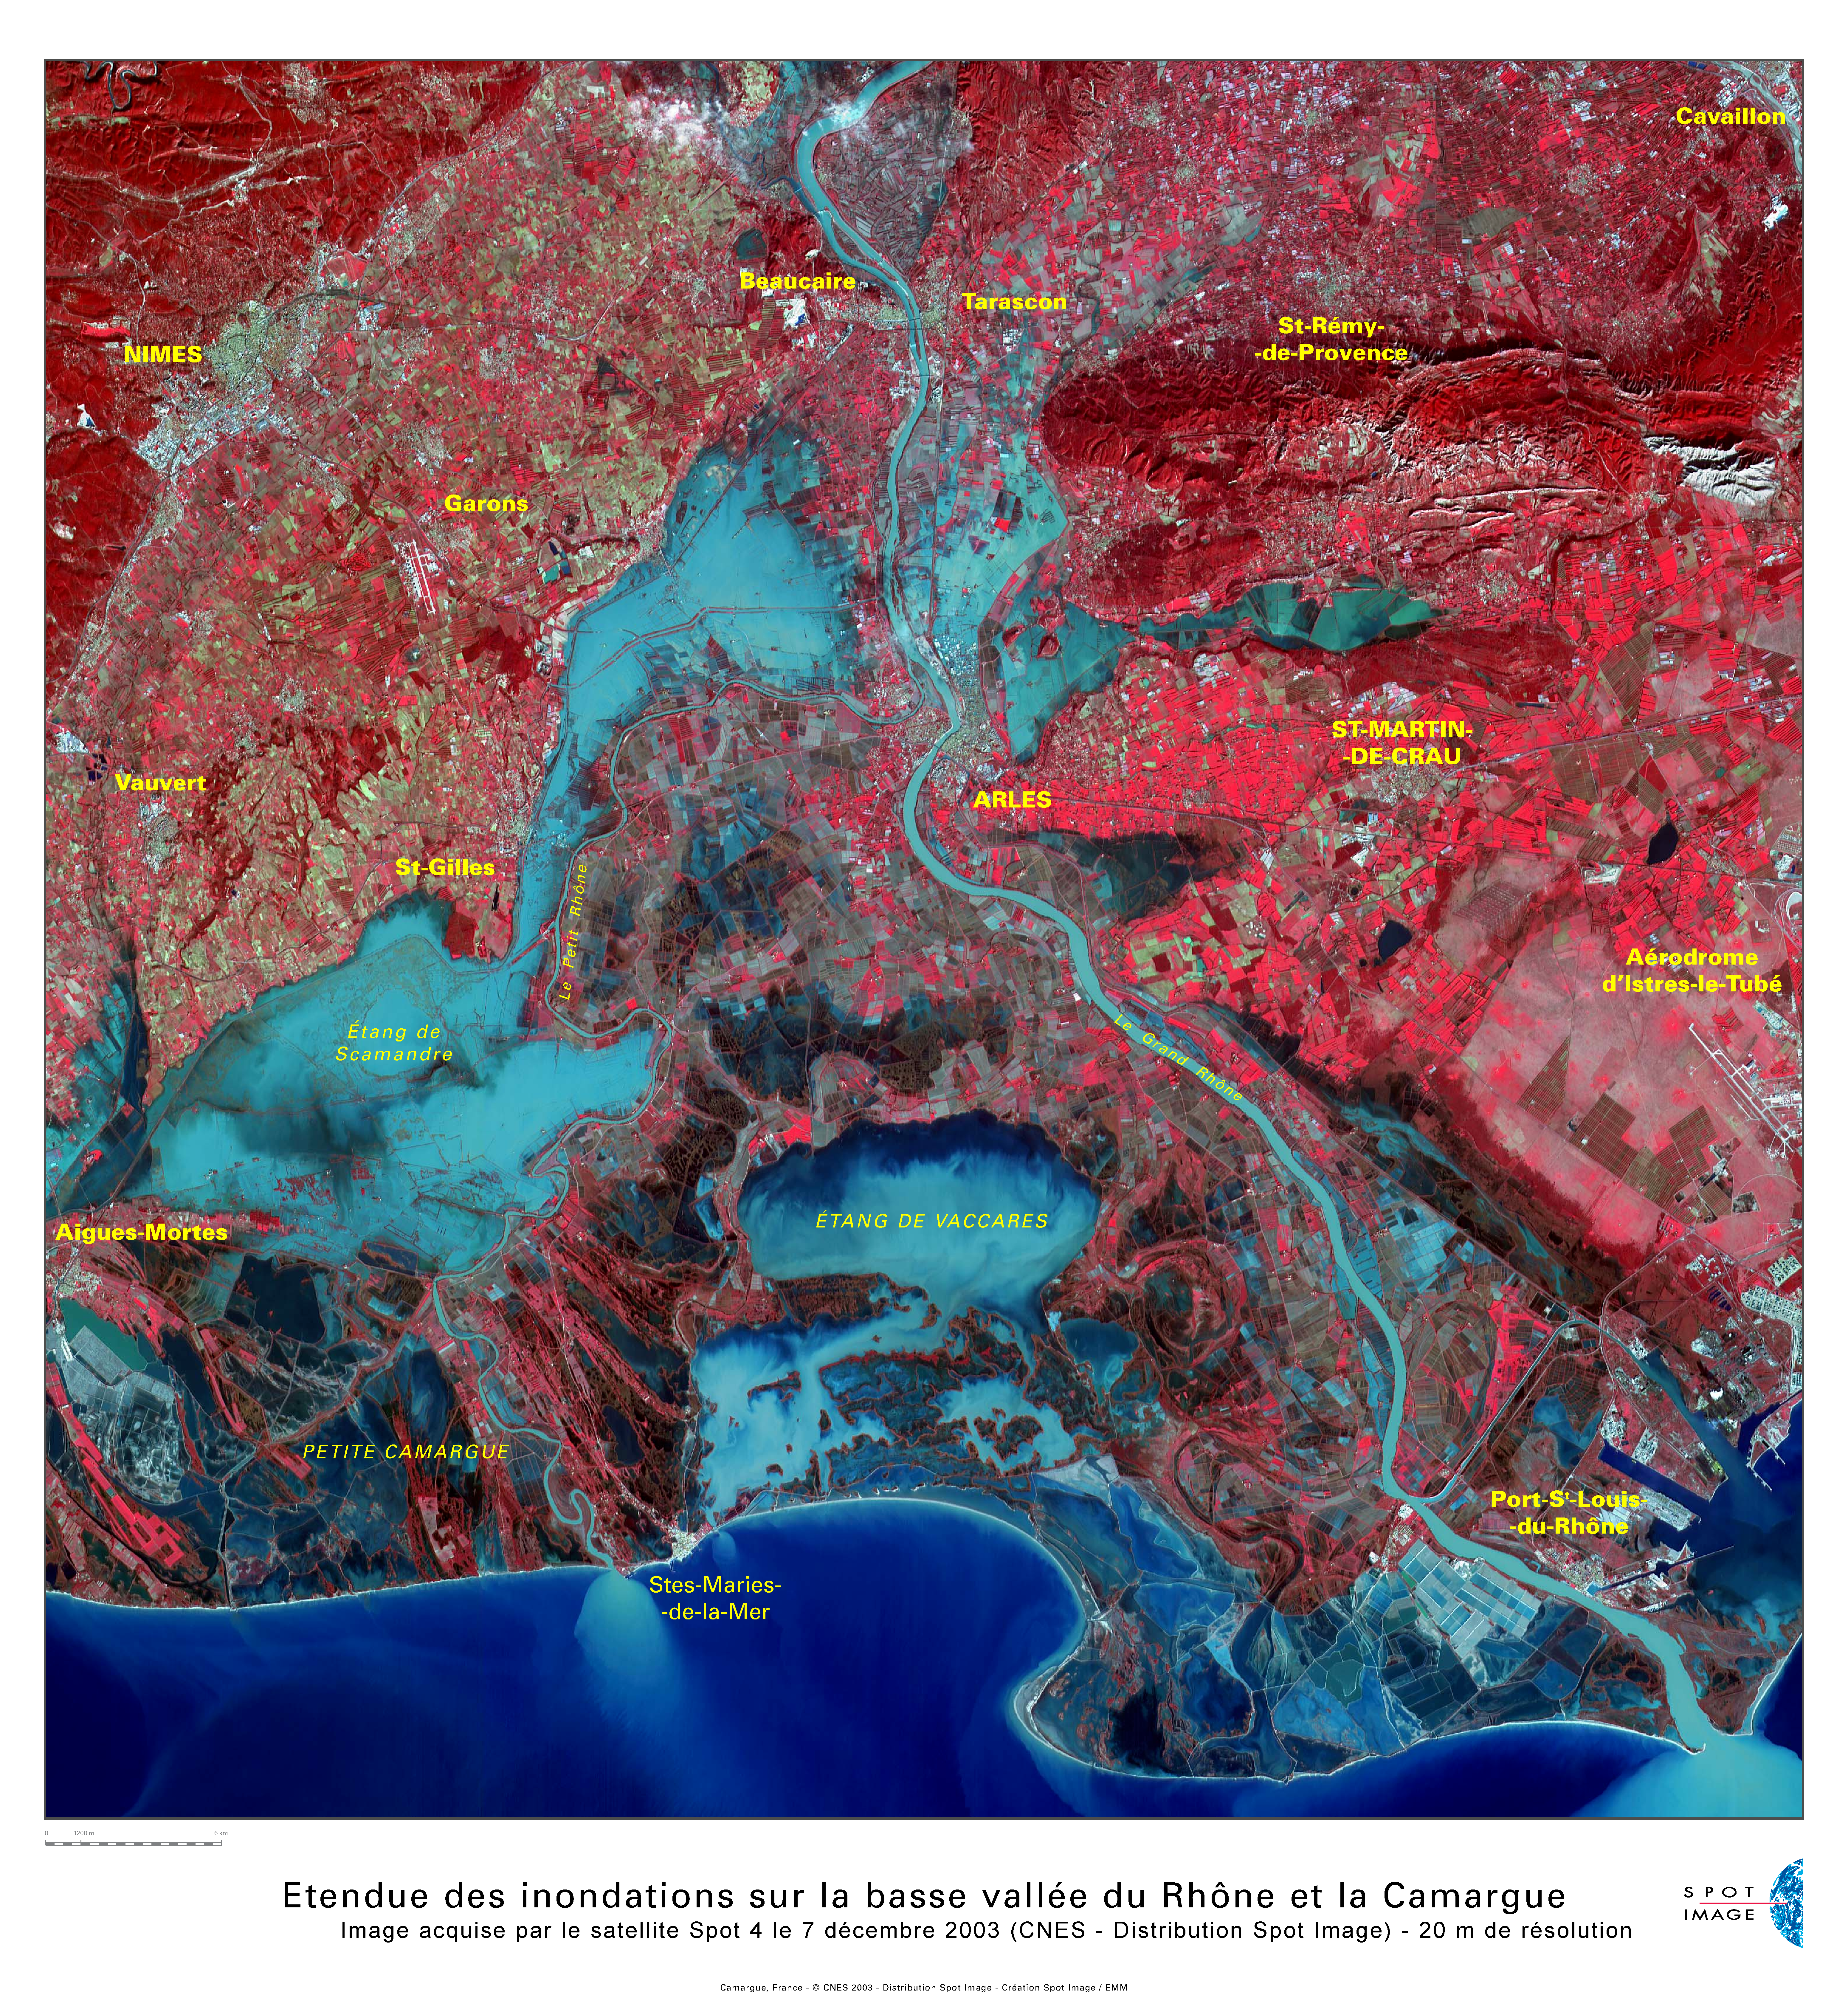
\includegraphics[width=.9\linewidth]{Chapitre1_Intro/Figures/SpotDec2003.pdf}	
	\caption{Image satellite de la basse vallée du Rhône le 7 décembre 2003, soit trois jour après la pointe de la crue. Les zones bleues représentent les cours d'eau ou les terres inondées, alors que les zones en rouge ou vert représentent des terrains secs. Source : CNES - Distribution Spot image.}
	\label{fig:Spot}
\end{figure}

\FloatBarrier
	\section*{Objectifs et organisation du manuscrit}
	\addcontentsline{toc}{section}{Objectifs et organisation du manuscrit}
%Là, tu peux citer les travaux qui ont cherché à dépasser ces limites, et indiquant tous les pbs qui restent non résolus. Et notamment l'utilisation de données historiques, LA piste prometteuse, mais en listant ce qui n'a pas été traité ou pas bien (incertitudes hydrométrie, méthodo intégrée de bout en bout, etc.).
%
%3/ expliquer ce que tu vas faire (objectifs et démarche scientifiques) : objectifs généraux, le site d'étude et pourquoi lui, l'organisation du manuscrit (il faut qu'on retrouve les grands points qui vont structurer les chapitres, et sur lesquels tu vas revenir en conclusion/perspectives).

	\paragraph{} La valorisation des données anciennes est l'un des moyens permettant d'améliorer les estimations des quantiles de crue extrêmes. La détermination et la propagation de l'ensemble des incertitudes lors de cet exercice est particulièrement importante mais elle est rarement effectuée. Un des objectifs de la thèse est de construire une méthode opérationnelle, complète et homogène, qui intègre les incertitudes à chaque étape de l'analyse fréquentielle afin de les propager jusqu'au résultat final. Dans ce contexte, l'utilisation de données historiques (pré-enregistrements continus) sera également explorée. L'utilisation de ces données est associée au concept de seuil de perception, qui est généralement supposé parfaitement connu dans la littérature. La prise en compte d'incertitudes affectant le seuil de perception et la durée de la période historique sera étudiée. La station hydrométrique du Rhône à Beaucaire constitue un cas d'étude idéal du fait de la longévité exceptionnelle des mesures de hauteur d'eau en continu (plus de deux siècles) et de l'immense patrimoine de données hydro-climatiques disponible dans la base de données HISTRHÔNE depuis le XIII \textsuperscript{ème} siècle. Les objectifs décrits ci-dessus seront étudiés dans ce manuscrit de thèse pour la station du Rhône à Beaucaire.
	
	\paragraph{} Ce manuscrit de thèse s'organise en trois parties dont les contours sont résumés dans la figure \ref{fig:SchemaThese}. Le premier chapitre permet de faire un bilan des données disponibles. Les relevés limnimétriques disponibles à Beaucaire depuis 1816  seront présentés en parallèle d'une étude de l'évolution des conditions d'écoulement de la zone au cours des deux derniers siècles. Les données de la base HISTRHÔNE jugées utiles à l'analyse fréquentielle des crues en seront extraites et des modèles hydrauliques seront utilisés pour tenter d'estimer le débit de ces événements anciens. 
	
	\paragraph{} Le second chapitre prend la forme d'un article scientifique soumis à "Journal of Hydrology" et accepté sous réserve de révision mineures. L'utilité des données limnimétriques historiques pour la réduction des incertitudes de l'analyse fréquentielle est explorée. La détermination et la propagation des différentes sources d'incertitude hydrométrique est effectuée pour la chronique du Rhône à Beaucaire de 1816 à 2020. On dispose alors d'une chronique continue de débits journaliers de plus de deux siècles. La part respective de l'incertitude hydrométrique et de l'incertitude d'échantillonnage au sein des estimations des quantiles de crue est ensuite examinée pour différentes tailles de chroniques. 
	
	\paragraph{} Le troisième chapitre reprend la série continue de débits de 1816 à 2020 estimée au chapitre précédent, ainsi que les données de la base HISTHRÔNE extraites au premier chapitre, afin de réaliser une analyse probabiliste des crues de 1500 à 2020. Le modèle probabiliste présenté dans ce chapitre permet de considérer les incertitudes de la chronique de débits continus (1816-2020), mais également la méconnaissance du seuil de perception et de la durée de la période historique. L'apport et les limites de l'utilisation des données historiques pour l'analyse fréquentielle des crues est explorée sous différentes hypothèses. 
	
	\paragraph{} Enfin une conclusion présente les principaux résultats et avancées obtenus pendant la thèse, puis des perspectives de travaux et études complémentaires.
	

\begin{figure}[h]
	\centering
	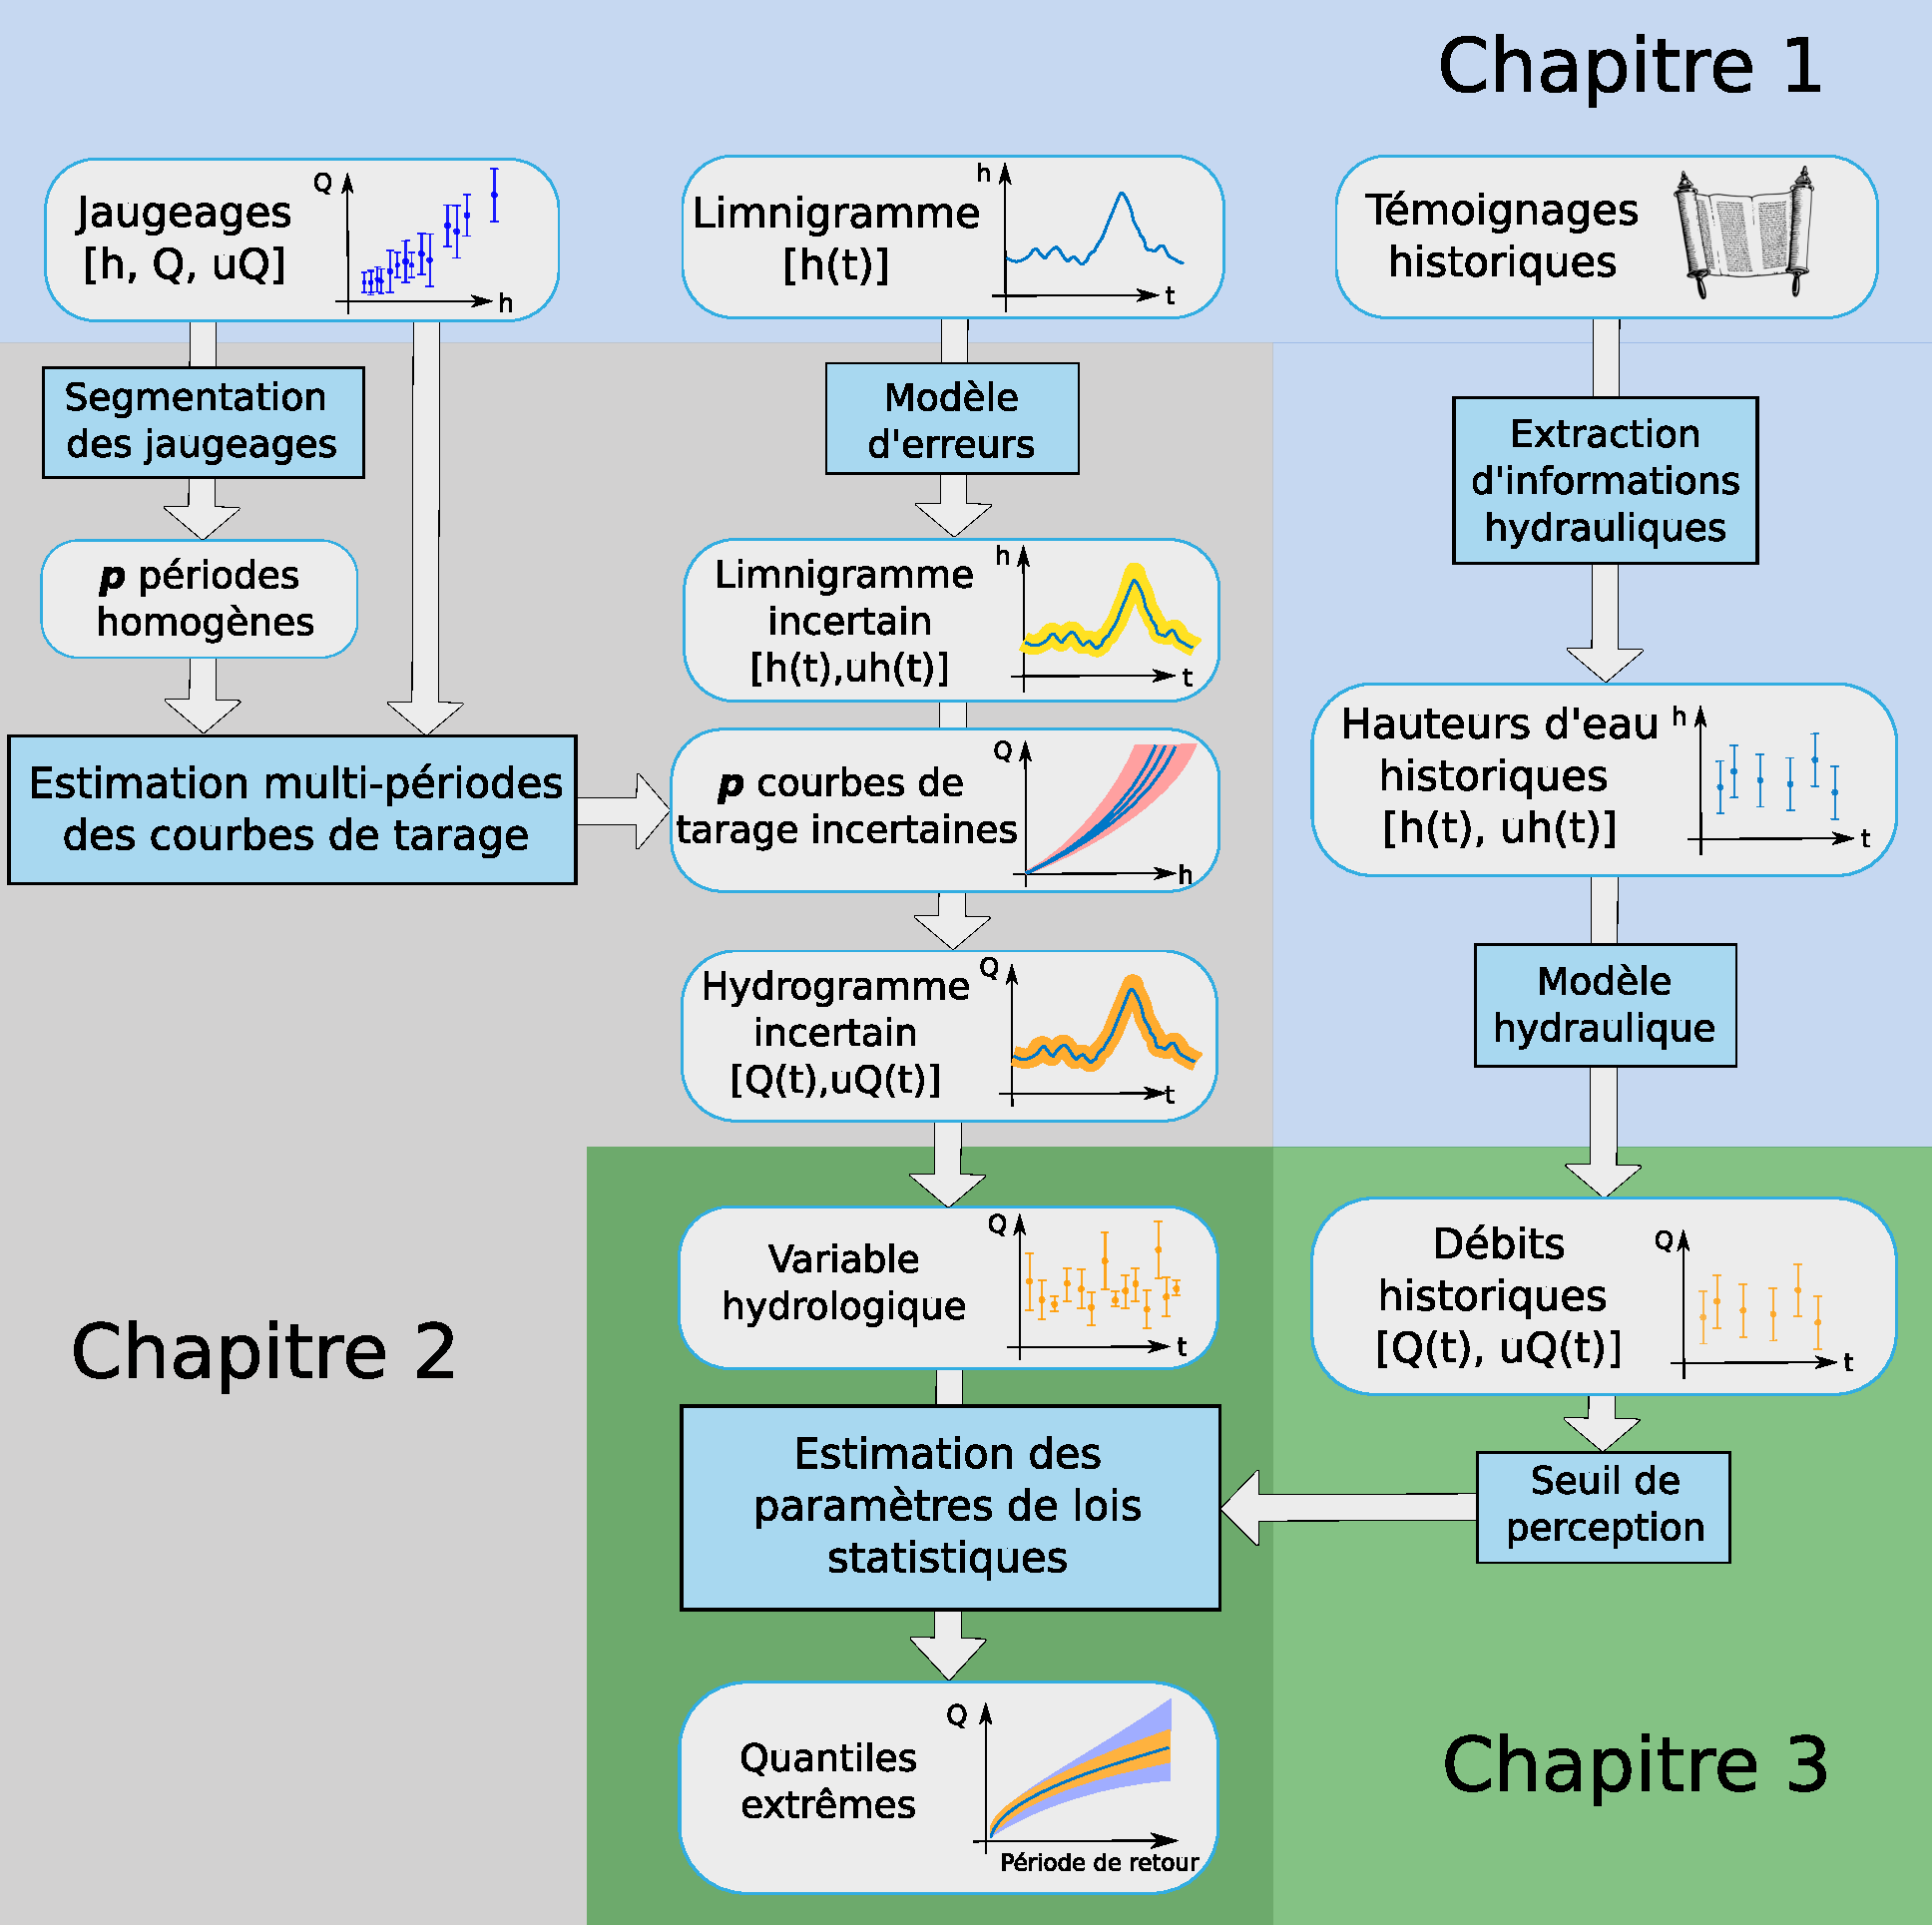
\includegraphics[width=.9\linewidth]{Chapitre1_Intro/Figures/SchemaThese.pdf}	
	\caption{Schéma d'organisation de la thèse. Les cases grises correspondent aux données et les cases bleues aux modèles et méthodes d'analyse. La lettre $h$ correspond à la hauteur d'eau, $Q$ au débit et $t$ au temps. La lettre $u$ correspond à l'incertitude qui affecte chacune de ces variables.}
	\label{fig:SchemaThese}
\end{figure}

\FloatBarrier

%\newpage
%%
%\printbibliography
%\end{document}

%\documentclass[11pt]{article}
%% packages
%\usepackage[utf8]{inputenc}
%\usepackage[french]{babel}
%\usepackage[T1]{fontenc}
%\usepackage{geometry}
%\usepackage[pdftex]{graphicx}
%\usepackage{graphicx}
%\usepackage{tabularx}
%\usepackage{dsfont}
%\usepackage{multirow}
%\usepackage{amsmath,amsfonts,amssymb}
%\usepackage{subcaption}
%\usepackage{authblk}
%\usepackage{placeins}
%\usepackage{epigraph}
%\usepackage{lscape}
%\usepackage{rotating}
%\usepackage{longtable}
%\usepackage{array, booktabs, ltablex, makecell, threeparttablex}
%
%%hyperlinks options
%\usepackage{hyperref}
%\hypersetup{colorlinks=true,linkcolor=blue,filecolor=magenta,urlcolor=cyan,citecolor=cyan}
%%bib options
%\usepackage[backend=biber,style=authoryear,bibstyle=authoryear,natbib=true,
%giveninits=true,uniquename=false,uniquelist=false,% firstinits=false,
%maxcitenames=2,date=year, maxbibnames=99,url=false]{biblatex}
%\geometry{left=20mm, top=20mm, right=20mm}
%%float barrier
%\usepackage{placeins}
% \addbibresource{Thèse.bib}
%\title{Chapitre 2 : Collecte et caractérisation des données de crue à Beaucaire}
%\author{Mathieu}
%
%\begin{document}
%\maketitle
%
%
%\tableofcontents
%
%
%\newpage 

%\section{Introduction}

\chapter{Collecte et caractérisation des données de crue à Beaucaire}
\label{chap:ch2}
\newpage

\section{Hydrométrie du Rhône à Beaucaire de 1816 à aujourd'hui}
\label{sec:hydrometrie}

\paragraph{} Le passé de Beaucaire, du XVII\textsuperscript{ème} au XIX\textsuperscript{ème} siècle était indéniablement tourné vers le commerce fluvial. La foire de Beaucaire, d'importance européenne, attirait alors des marchands venus des quatre coins de la Méditerranée (figure \ref{fig:foire}). La ville de Beaucaire était considérée comme «\textit{la capitale française des marchandises}» \citep{leon_vie_1953} grâce à sa proximité avec la mer et les échanges fluviaux rendus possibles par son port sur le Rhône. L'attention des Beaucairois était alors tournée continuellement vers le fleuve et ses caprices. Les crues et étiages fréquents perturbaient le commerce fluvial, source principale des revenus beaucairois avant l'avènement du chemin de fer. A cette époque, Beaucaire et Tarascon étaient reliées par un pont de bateaux, qui, jusqu'à la construction d'un pont en pierre en 1830, servait à passer d'une ville à l'autre. Ce pont était régulièrement détruit par les crues, comme en 1745 : «\textit{le pont de bateaux de Tarascon alla heurter et emporter celui d'Arles}» \citep{anibert_annales_1764}. Du fait de cet intérêt majeur pour le fleuve, le Rhône à Beaucaire fut l'une des premières stations limnimétriques françaises avec des relevés continus dès le début du XIX\textsuperscript{ème} siècle. 

\begin{figure}[h]
		\centering
            \begin{subfigure}{0.49\linewidth}
            \centering
            	\includegraphics[width=1\linewidth]{Chapitre2/Figures/foire4.jpg}\hfill
            	\caption{}
            	\label{subfig:foire1}
            \end{subfigure}
            \begin{subfigure}{0.49\linewidth}
            \centering
            	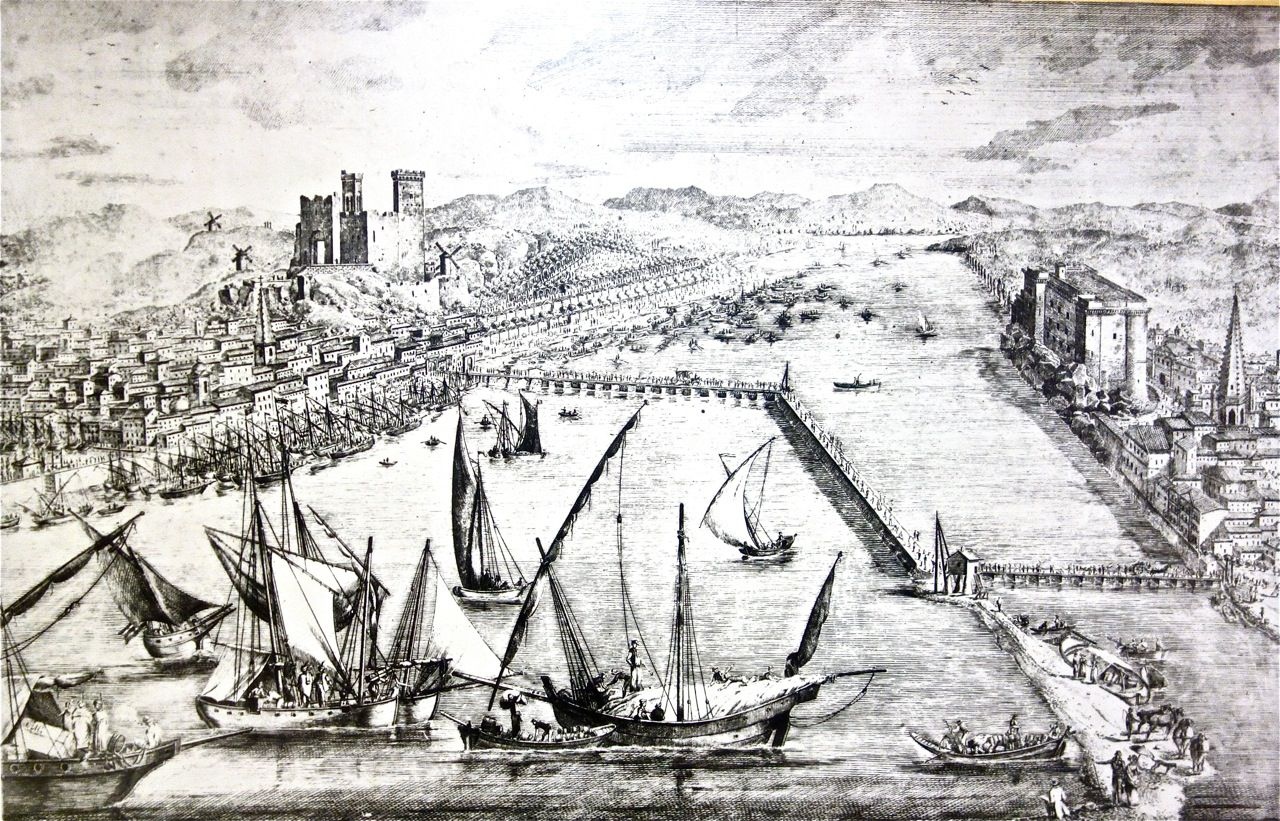
\includegraphics[width=1\linewidth]{Chapitre2/Figures/foire5.jpg}
            	\caption{}
           		\label{subfig:foire2}
            \end{subfigure}
\caption{(a) «\textit{Vue de la foire de Beaucaire avec une partie de la ville de Tarascon}», Basset André (1749). On distingue la ville de Beaucaire sur la droite et Tarascon sur l'autre rive. 
(b) Pont de bateaux reliant Beaucaire à Tarascon lors de la foire, auteur inconnu (XVIII\textsuperscript{ème} siècle). Le pont était alors régulièrement détruit lors des crues, empêchant toute communication entre les deux villes.}
\label{fig:foire}
\end{figure}

\FloatBarrier
	\subsection{Contexte hydrologique et hydrométrique}
	
	\paragraph{} Le Rhône à Beaucaire draine un bassin versant de 95~590 km² et son module est de 1680 m\textsuperscript{3}/s (1920-2023) \citep{medd_banque_2021}. La station hydrométrique de Beaucaire est la station la plus à l'aval du Rhône dit "complet" car elle est située 5 km à l'aval de la confluence avec le Gardon (dernier affluent significatif du Rhône), et 10 km à l'amont de la diffluence qui donne naissance au Petit-Rhône et au Grand-Rhône (figure \ref{fig:BV}). Il s'agit donc de la station mesurant le débit le plus important du fleuve, mais également de France, le Rhône étant le premier fleuve français en termes de débit. Au delà de son important débit, le Rhône est un fleuve complexe par la diversité de ses apports. Comme décrit par \citet{parde_regime_1925}, il comporte « \textit{ une infinité de nuances et de contrastes, la Massa, l'Arve, l'Isère, la Durance, l'Ain, la Saône, l'Ardèche, c'est-à-dire des cours d'eau appartenant à toutes les catégories qu'on puisse trouver en Europe occidentale. [...] Ainsi, c'est par une carrière agitée que le petit torrent glaciaire de Gletsch devient le fleuve majestueux de Beaucaire, tour à tour ou en même temps nival et séquanien, océanique et méditerranéen, pondéré ou sujet aux plus déconcertants accès de démence} ». À Beaucaire, les signatures des affluents alpins, océaniques, méditerranéens et cévenols se mélangent pour donner naissance à un régime hydrologique qu'il est difficile de classer dans une catégorie (figures \ref{fig:Regime} et \ref{fig:RegimeAffluents}). Il en est de même pour les crues, qui sont le reflet de la complexité de ses apports : « \textit{Il est violent par son courant encore inapaisé tout près de la Méditerranée, par ses crues de plus en plus nombreuses, désordonnées et massives, à mesure qu'il approche du terme de son cours} » \citep{parde_regime_1925}. 
	
		\begin{figure}[h!]
	\centering
		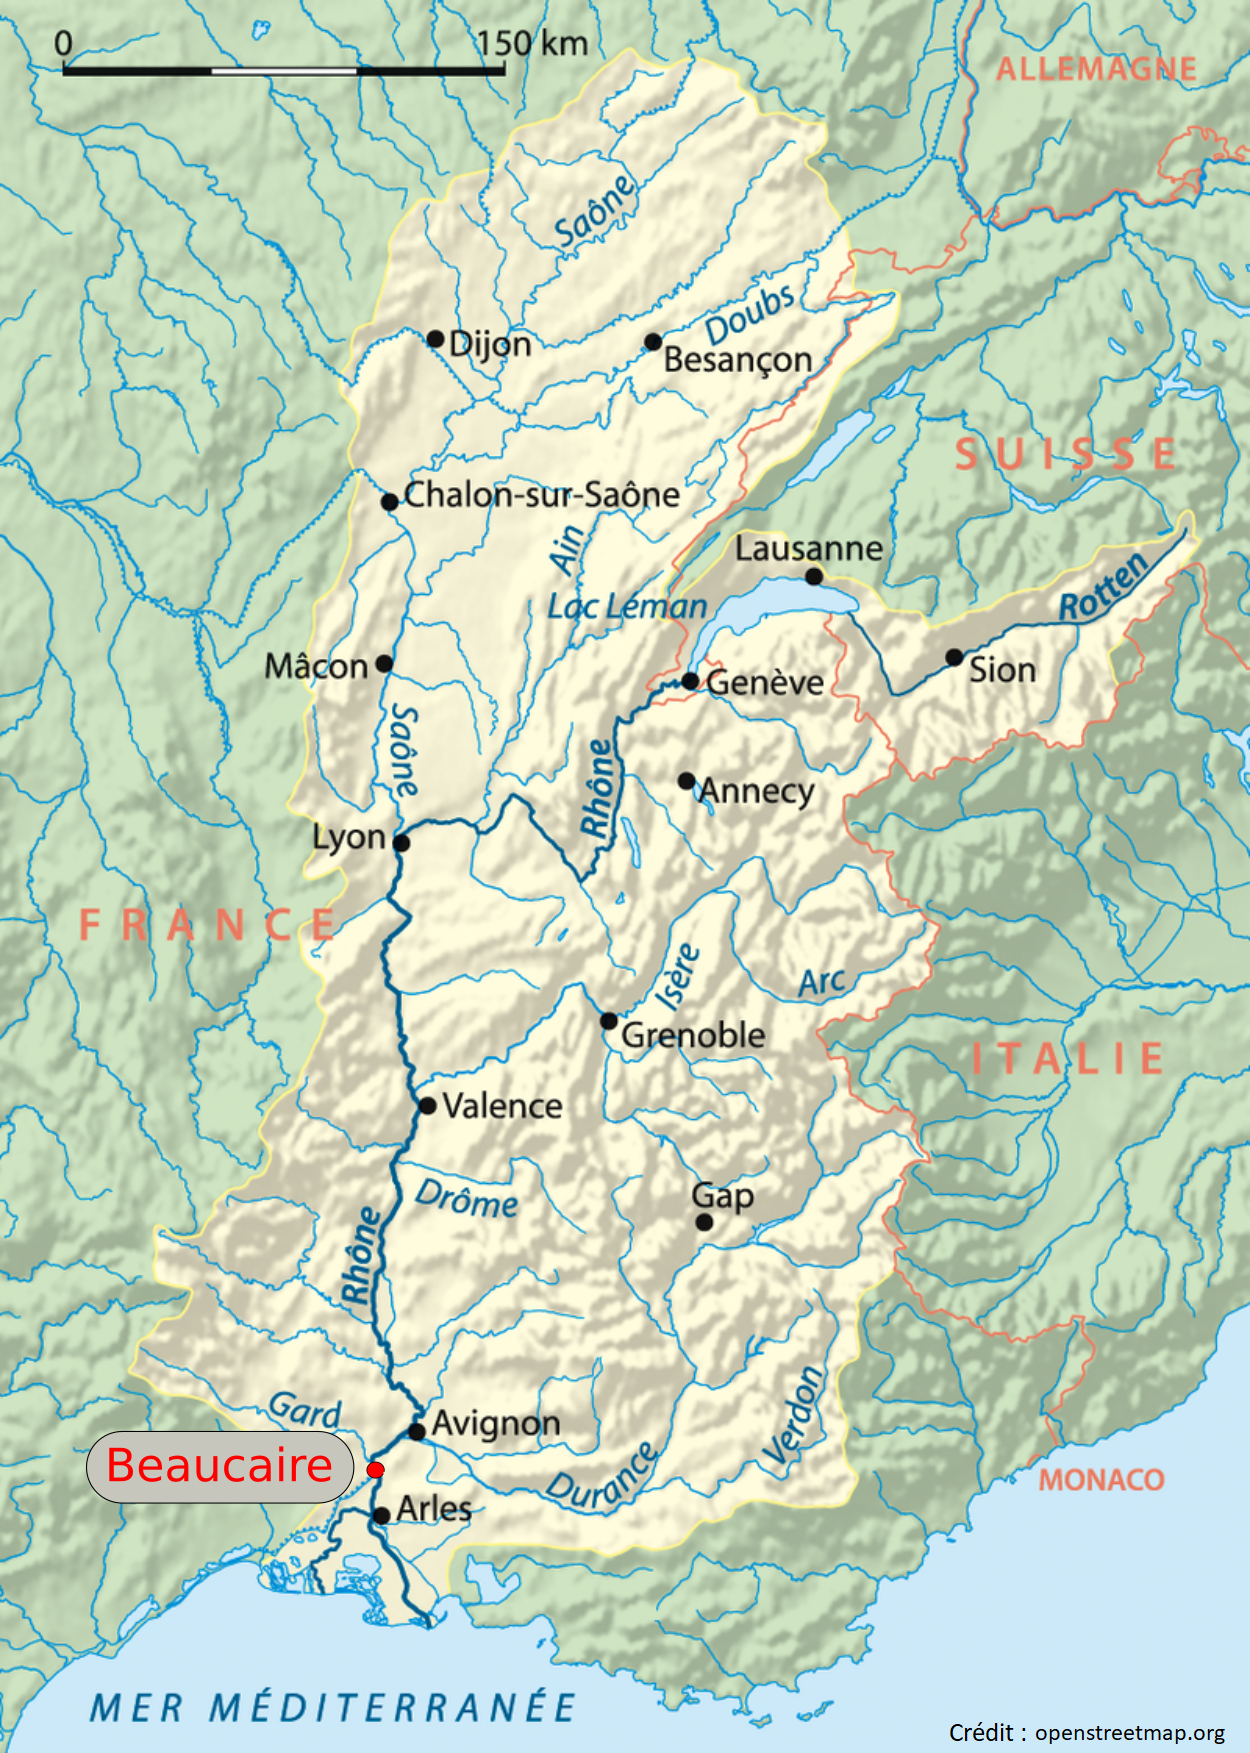
\includegraphics[width=.5\linewidth]{Chapitre2/Figures/Rhone_bassin_versant.png}
        \caption{Bassin versant du Rhône. La ville de Beaucaire est indiquée en rouge (www.openstreetmap.org)}	
		\label{fig:BV}
	\end{figure}
	
	\begin{figure}[h!]
	\centering
		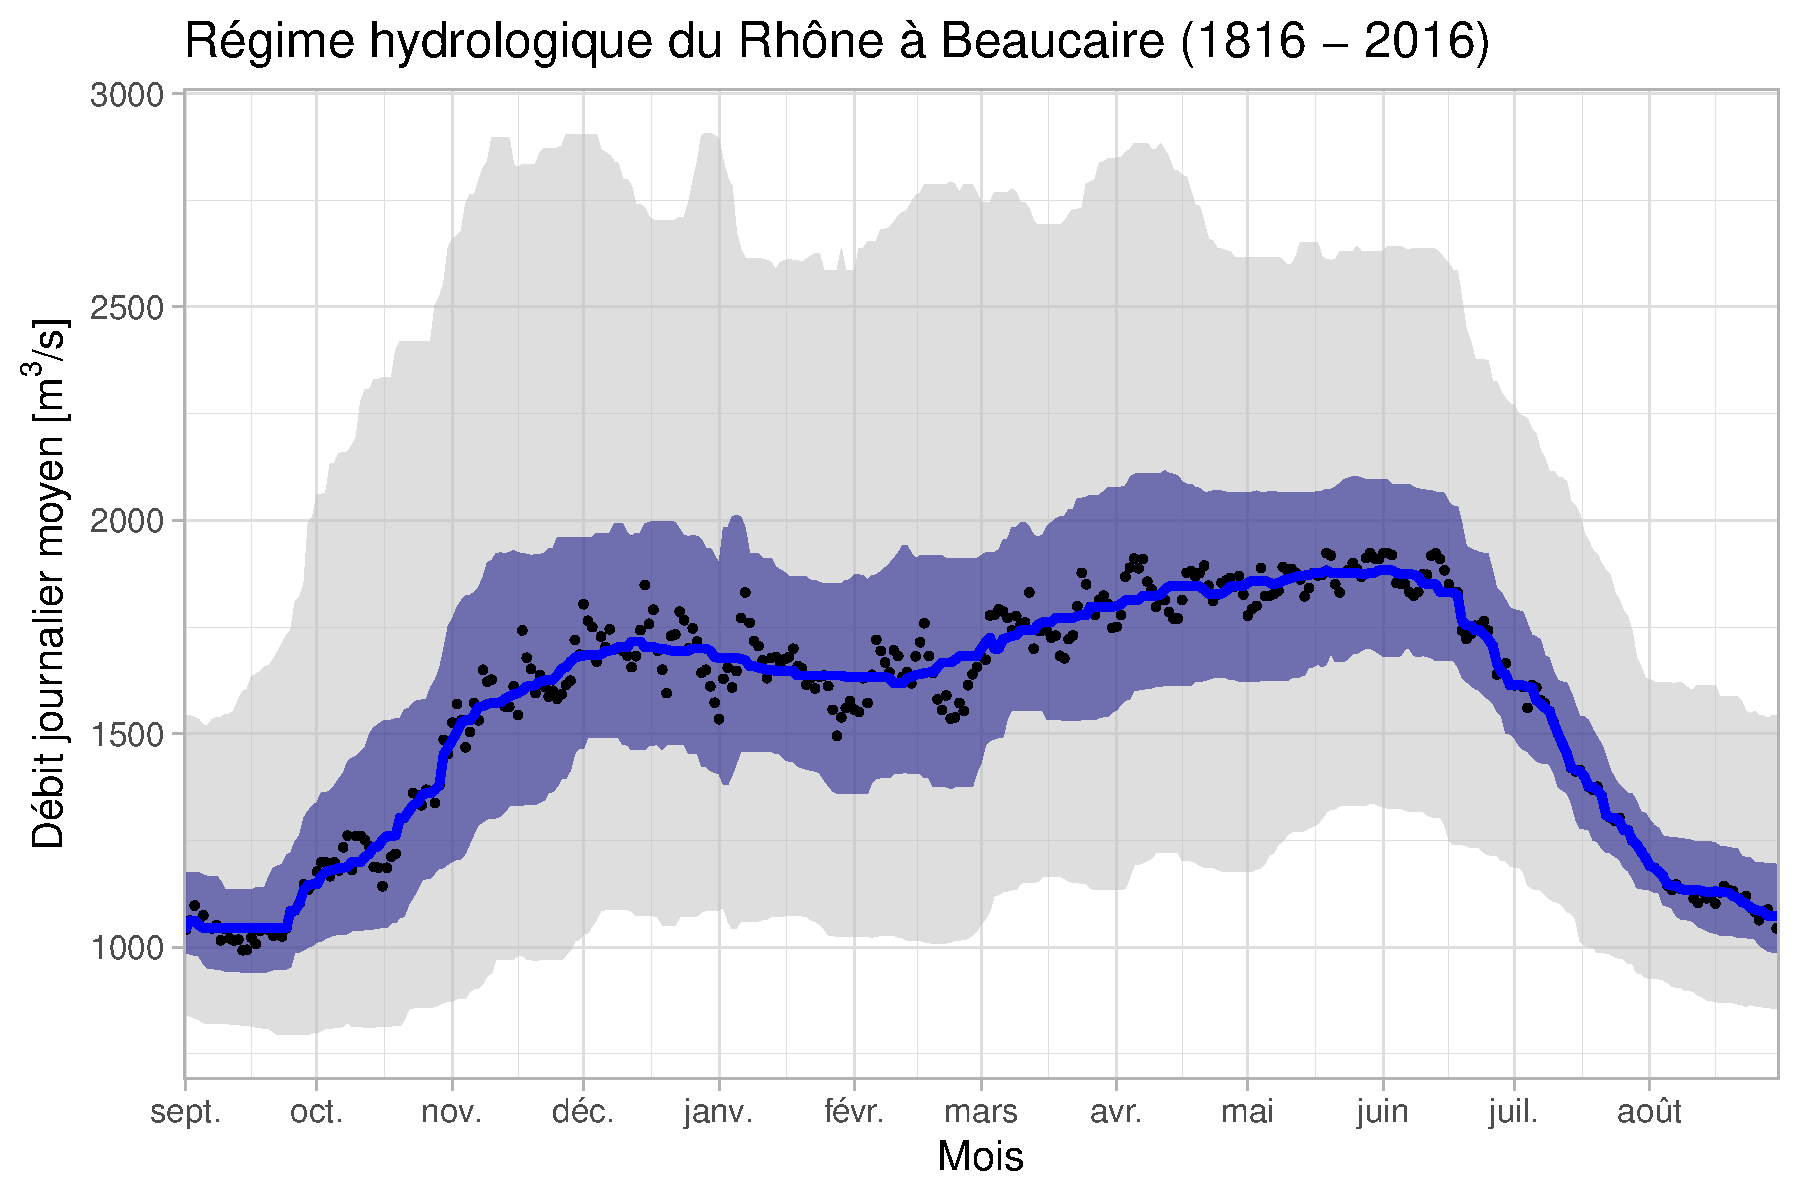
\includegraphics[width=.7\linewidth]{Chapitre2/Figures/Regime.pdf}
        \caption{Débits moyens journaliers du Rhône à Beaucaire de 1816 à 2016 (points noirs). En bleu foncé, les quantiles 40 et 60\%, en gris les quantiles 20 et 80\%. La courbe bleue représente la médiane.}	
		\label{fig:Regime}
	\end{figure}
	
	\begin{figure}[h!]
	\centering
		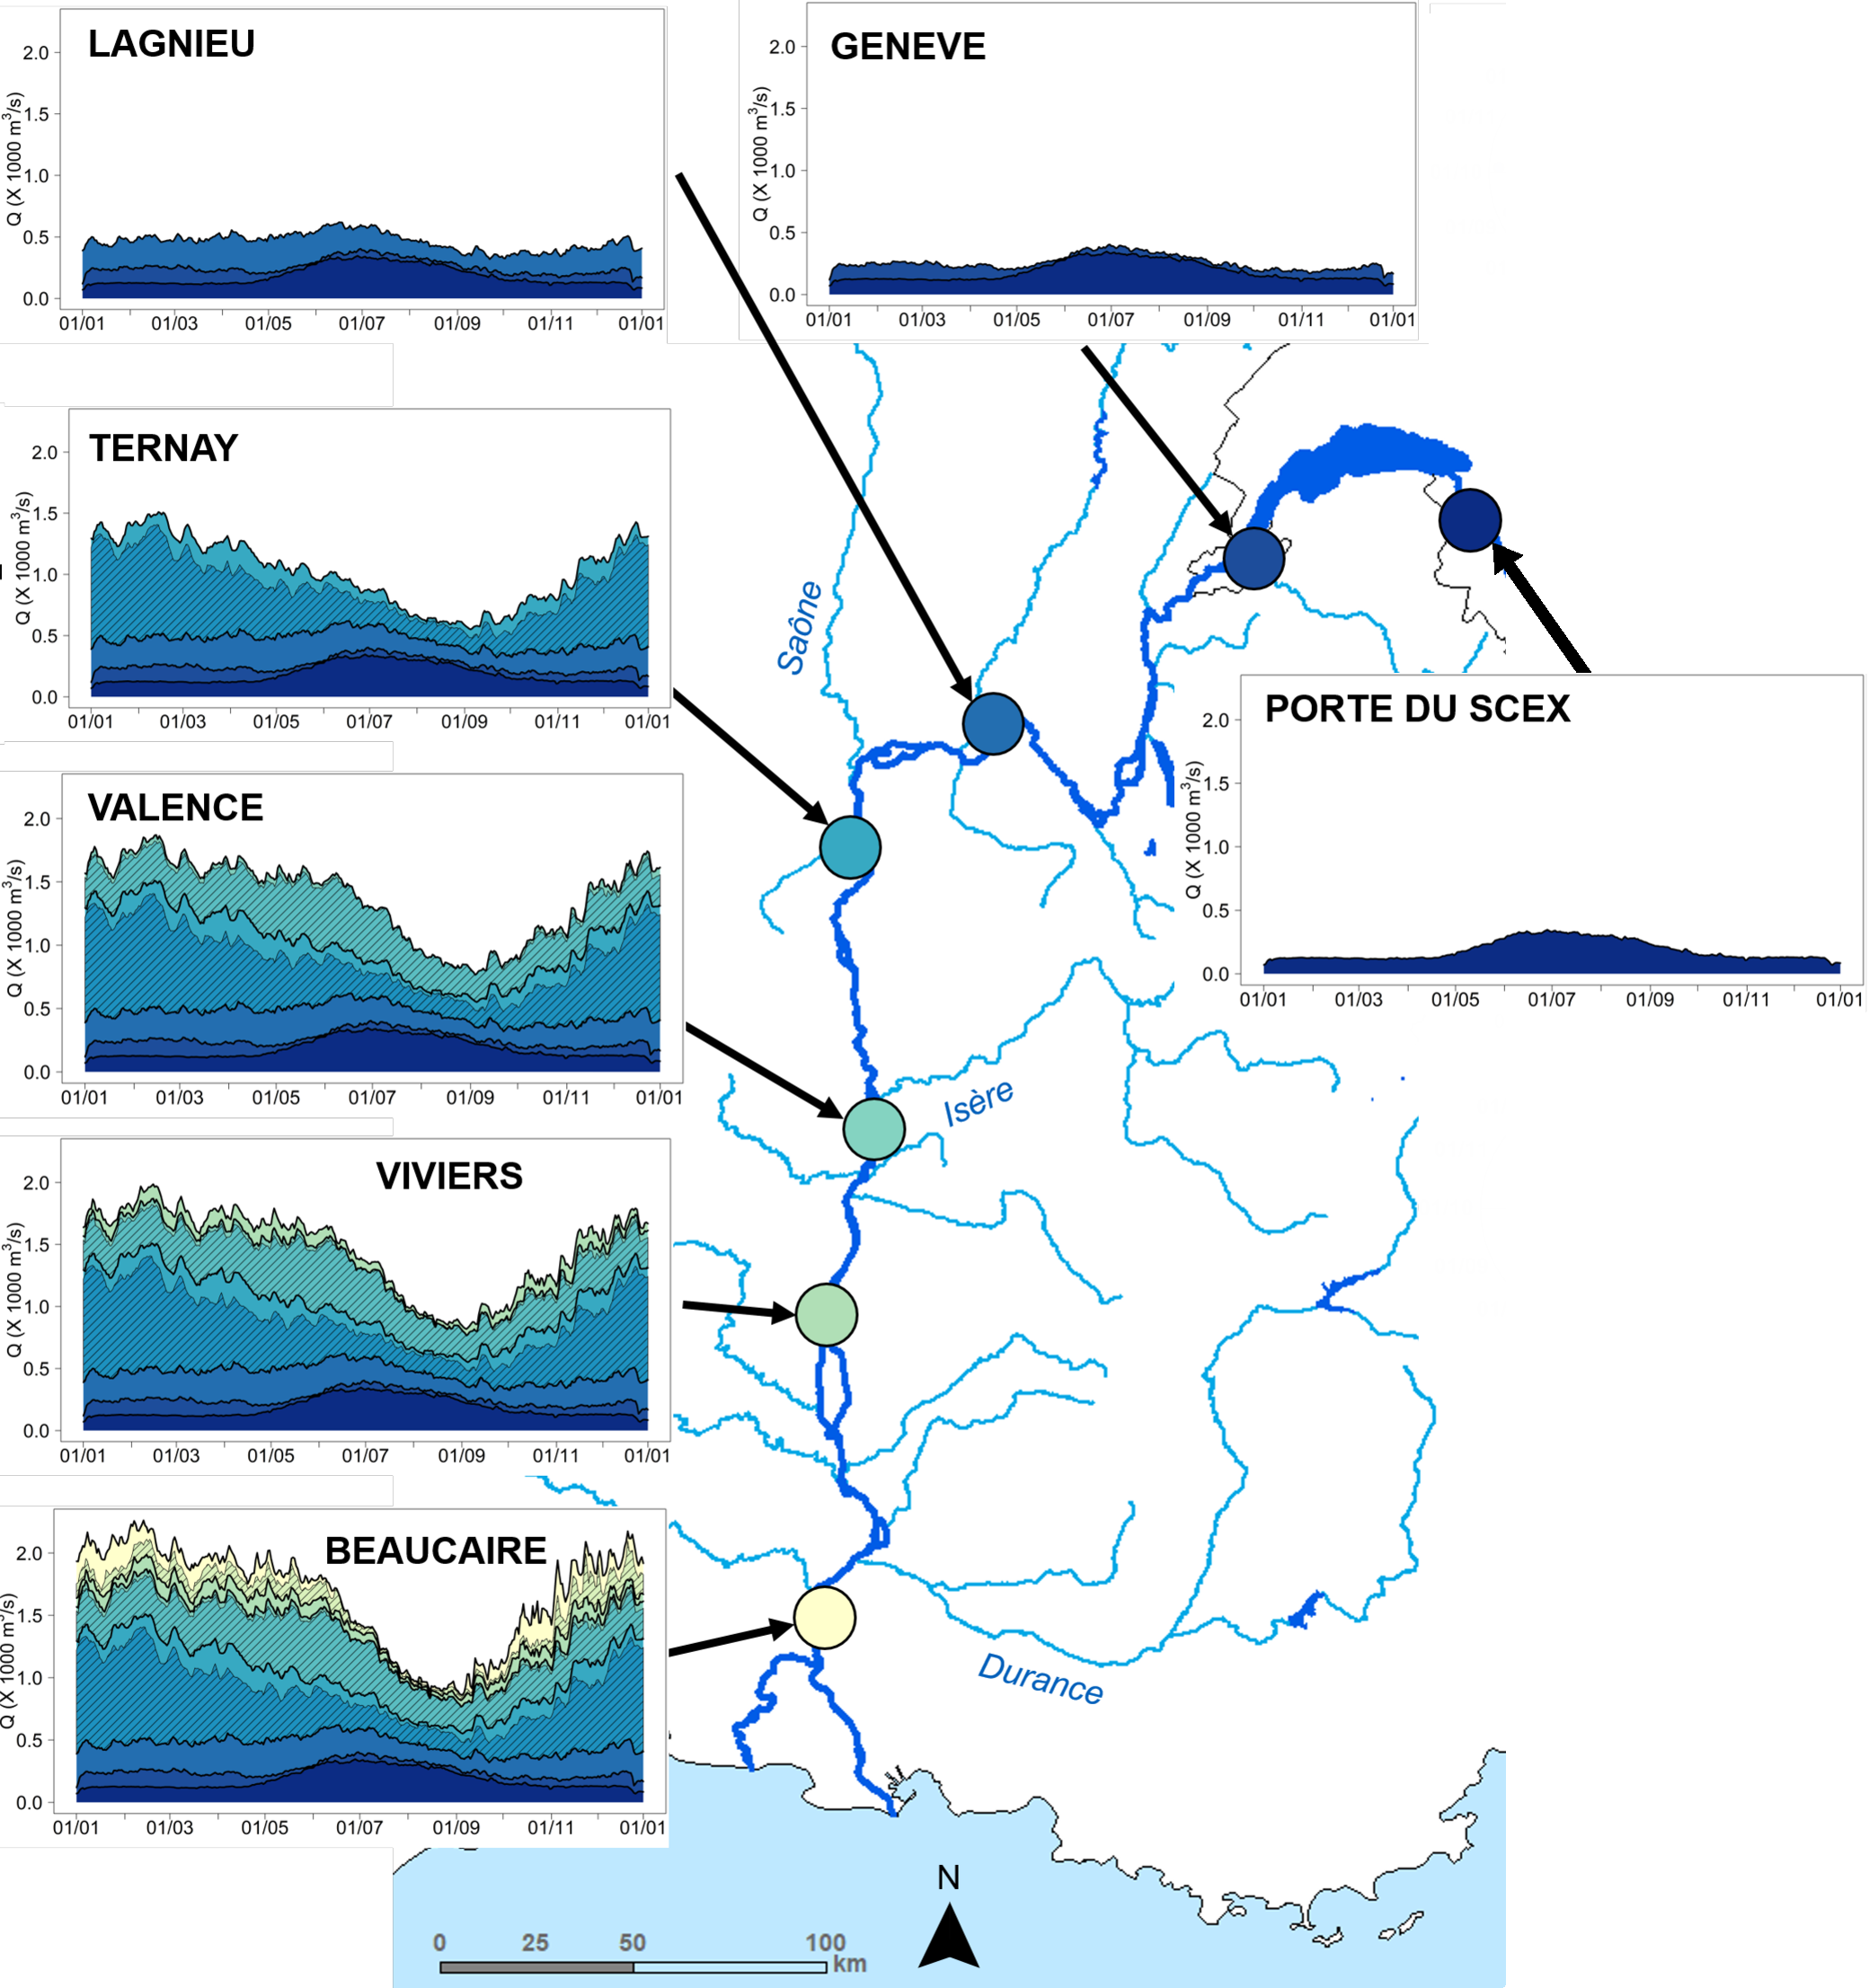
\includegraphics[width=.6\linewidth]{Chapitre2/Figures/RégimeRhône.pdf}
        \caption{Évolution du régime hydrologique du Rhône aux différentes stations hydrométriques. Les hydrogrammes décrivent les débits journaliers moyens interannuels. Les graphiques font apparaitre les contributions des stations situées en amont ainsi que celles des principaux affluents français : Saône, Isère et Durance (identifiées par des hachures). Figure adaptée de \cite{le_coz_flux_2023}, à paraître.}	
		\label{fig:RegimeAffluents}
	\end{figure}

	\paragraph{} Au cours des deux derniers siècles, trois crues apparaissent comme particulièrement marquantes. Tout d'abord l'événement du 3 novembre 1840 est probablement le plus important depuis le début du XIX\textsuperscript{ème} siècle. Il est décrit par \citet{parde_regime_1925} comme «\textit{l'événement météorologique le plus grandiose et le plus déconcertant qui se soit jamais produit dans le bassin du Rhône}». Les dégâts sont généralisés : le centre ville de Lyon est sous les eaux, la concomitance avec la crue de la Durance entraine de nombreux dégâts à Avignon et la Camargue est complètement inondée suite à de nombreuses brèches dans les digues. \citet{parde_regime_1925} donne une estimation de débit à 13~000~m\textsuperscript{3}/s à Beaucaire. Vient ensuite la crue du 31 mai 1856 qui touche non seulement le Rhône, mais également de nombreux cours d'eau français dont la Loire. \citet{parde_regime_1925} la décrit comme «\textit{la plus simple et la plus brutale des crues générales du Rhône}» et estime son débit à Beaucaire à 12~500~m\textsuperscript{3}/s. A nouveau, les dégâts sont colossaux de Lyon à la mer. Ces deux crues de période de retour supérieure à 100 ans sont encore aujourd'hui des références pour l'estimation du risque inondation. Jusqu'en décembre 2003, aucun événement ne s'en était réellement approché et les risques de débordements majeurs et de ruptures de digues avaient été peu à peu oubliés. Avec ses 11~500~m\textsuperscript{3}/s qui correspondent à une période de retour centennale \citep{medd_debit_2005}, la crue de 2003 a ravivé les craintes des populations provençales. Au cours de l'événement, plusieurs digues supposées résister à des niveaux similaires à ceux de 1856 cèdent et provoquent l'inondation des foyers de plus de 8000 personnes. Suite à cet événement, une stratégie d'aménagement pour la prévention du risque inondation est mise en place (\url{www.plan-rhone.fr}) et de nombreuses digues sont rehaussées, notamment à l'aval de Beaucaire \citep{symadrem_programme_2012}. 
	
	
\FloatBarrier

	\subsection{Station hydrométrique du Rhône à Pont de Beaucaire (1816-1967)}
		
	\paragraph{} Le travail d'archive de \citet{pichard_les_1995} et \citet{pichard_hydro-climatology_2017} a permis de reconstituer une chronique continue d'observations de la hauteur d'eau du Rhône à Beaucaire à partir du 15 mai 1816 (tableau \ref{tab:MesuresPtBcr}). Ces relevés semble être les plus anciens qu'il soit possible de retrouver à Beaucaire (\cite{parde_regime_1925}; \cite{pichard_les_1995}). L'échelle limnimétrique fut installée au point kilométrique 267.7, sur le musoir de l'écluse du canal de Beaucaire à la mer dont les travaux furent achevés en 1811 (figure \ref{fig:CartoPt}). \citet{pichard_hauteurs_2013} souligne que «\textit{la longévité et la stabilité de cette échelle est (sic) évidemment exceptionnelle pour le bas Rhône. [...] La documentation chiffrée y est aussi précieuse et abondante qu'à Arles, mais cependant toujours aussi dispersée et accessible la plupart du temps par copie et non par les feuilles d'observations originales que les organismes gérants n'ont pas su conserver, en raison de transferts permanents d'attributions}». Il faut noter que l'écluse du canal de Beaucaire fut remplacée entre 1914 et 1918 par une autre écluse débouchant plus à l'aval. Il semble cependant que le musoir que l'on observe de nos jours existait dès l'origine du canal et que l'échelle n'a subi aucun déplacement (\cite{pichard_hauteurs_2013}; \cite{bard_actualisation_2018}). 
	
	\begin{figure}[h]
	\centering
		\includegraphics[width=.9\linewidth]{Chapitre2/Figures/CartoPt.pdf}
        \caption{(Gauche) Localisation de la station de Pont de Beaucaire (carte IGN 1950, source : www.geoportail.fr). (Droite) Échelle et limnigraphe CNR de Pont de Beaucaire en février 2020.}	
		\label{fig:CartoPt}
	\end{figure}

\FloatBarrier

	\subsubsection{Données disponibles}
	\paragraph{} Les relevés limnimétriques les plus anciens correspondaient probablement à une lecture d'échelle quotidienne en milieu de journée \citep{pichard_hauteurs_2013}. Après la crue généralisée de 1840 et la création du Service Spécial du Rhône, une norme de trois relevés par jour (à 7h, 12h et 17h) se met lentement en place (figure \ref{fig:RelevesPt}). L'application de cette norme n'est visible dans les données qu'à partir de 1887, et ce jusqu'à la fin de l'exploitation de la station.  L'année 1967 marque le début des travaux d'aménagement de l'ouvrage hydroélectrique de Vallabrègues et de son canal de dérivation, réalisés par la Compagnie Nationale du Rhône (CNR). Cette dérivation étant restituée à l'aval de la ville de Beaucaire, la station est déplacée 2 km plus à l'aval, environ 600 m à l'aval de la restitution des débits transitant par la centrale hydroélectrique. La nouvelle station, exploitée par la CNR à partir de 1970, sera alors appelée "Beaucaire Restitution", et sera décrite en détail dans la section \ref{subsec:Restit}. Le détail des relevés est indiqué dans le tableau \ref{tab:MesuresPtBcr}. Au final, ce sont plus de 200 ans de données limnimétriques continues qui sont disponibles à Beaucaire, et qui permettront une estimation du débit en continu sur cette période (chapitre \ref{chap:ch3}). 
	
	\begin{figure}[h]
          \centering
            \begin{subfigure}{0.49\linewidth}
            \centering
            	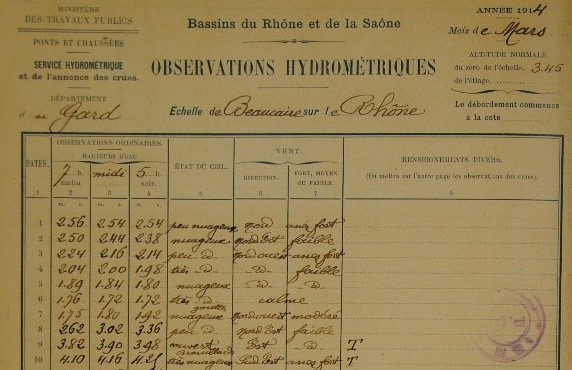
\includegraphics[width=1\linewidth]{Chapitre2/Figures/TabObsBcrSmall.jpg}\hfill
            	\caption{}
            	\label{subfig:TabObsPt}
            \end{subfigure}
            \begin{subfigure}{0.49\linewidth}
            \centering
            	
\includegraphics[width=1\linewidth]{Chapitre2/Figures/RegleStationCNR}
            	\caption{}
           		\label{subfig:RegleCNR}
            \end{subfigure}
      \caption{(a) Feuille originale des relevés de hauteur d'eau à Beaucaire réalisés par le service spécial du Rhône en mars 1914. On remarque les trois relevés par jour ainsi que des précisions sur l'état du ciel ou le vent. (b) Règles d'exploitation de la station de Pont de Beaucaire, fiche station de la CNR. On remarque que des observations horaires sont effectuées au-delà d'une certaine cote dont la valeur n'est pas indiquée (Source : Archives CNR, 1962)}
	 \label{fig:RelevesPt}
	\end{figure}            
            
    
	\begin{table}[h]
	\centering
	\caption{Détail des relevés limnimétriques des stations de Beaucaire}
    \label{tab:MesuresPtBcr}
	\resizebox{\columnwidth}{!}{%  
       \begin{tabular}{|m{2cm}| m{1.8cm} | m{2cm}| m{2cm} | m{2.5cm} | m{2.5cm} | m{2.5cm} |} 
%       {|c|c|c|c|c|c|c|}
%       {| m{2cm} | m{2.7cm}| m{2.2cm} | m{2.8cm} | m{2.9cm} | m{2.5cm} |} 
                \hline
               Nom & Période & Périodicité & Méthode & Origine & Zéro échelle & Commentaire \\
                \hline
                Pont de Beaucaire & 1816-1886 & 1 mesure/jour & Visuelle & 
                Service Spécial du Rhône & 3.37 mNGF IGN69  & Probablement mesure à 12h \\
                \hline
                Pont de Beaucaire & 1887-1967 & 3 mesures/jour & Visuelle & 
                Service Spécial du Rhône & 3.37 mNGF IGN69 & Relevés à 7h, 12h, 17h\\
                \hline
               Beaucaire Restitution & 1970-2020 & Horaire & Limnigraphe à flotteur puis LPN8 & 
                BD CNR & 0.06 mNGF IGN69  &  \\
                \hline
		\end{tabular}
		}
       \end{table}       
       
   
       
    \paragraph{} Les jaugeages les plus anciens récupérés dans les archives départementales du Rhône datent de 1845 (figure \ref{fig:Jau1845}) alors que les mesures limnimétriques débutent en 1816. Il faut noter que les jaugeages étaient effectués à l'amont de la ville de Beaucaire, au PK 264.5, dans une zone plus stable et dépourvue d'îles indiquée sur la figure \ref{fig:CartoPt}. Quatre jaugeages des années 1845 et 1846 font exception à la règle et ont été effectués au droit de la station. Un total de 233 jaugeages est disponible à Pont de Beaucaire, couvrant la période 1845-1967 (visibles sur la figure \ref{fig:JauAll}), avec une fréquence peu homogène et des périodes non jaugées (notamment en période de guerre). La plupart des jaugeages étaient effectués avec un moulinet embarqué sur un bateau, quelques jaugeages aux flotteurs existent également. 
    
    \begin{figure}[h]
	\centering
		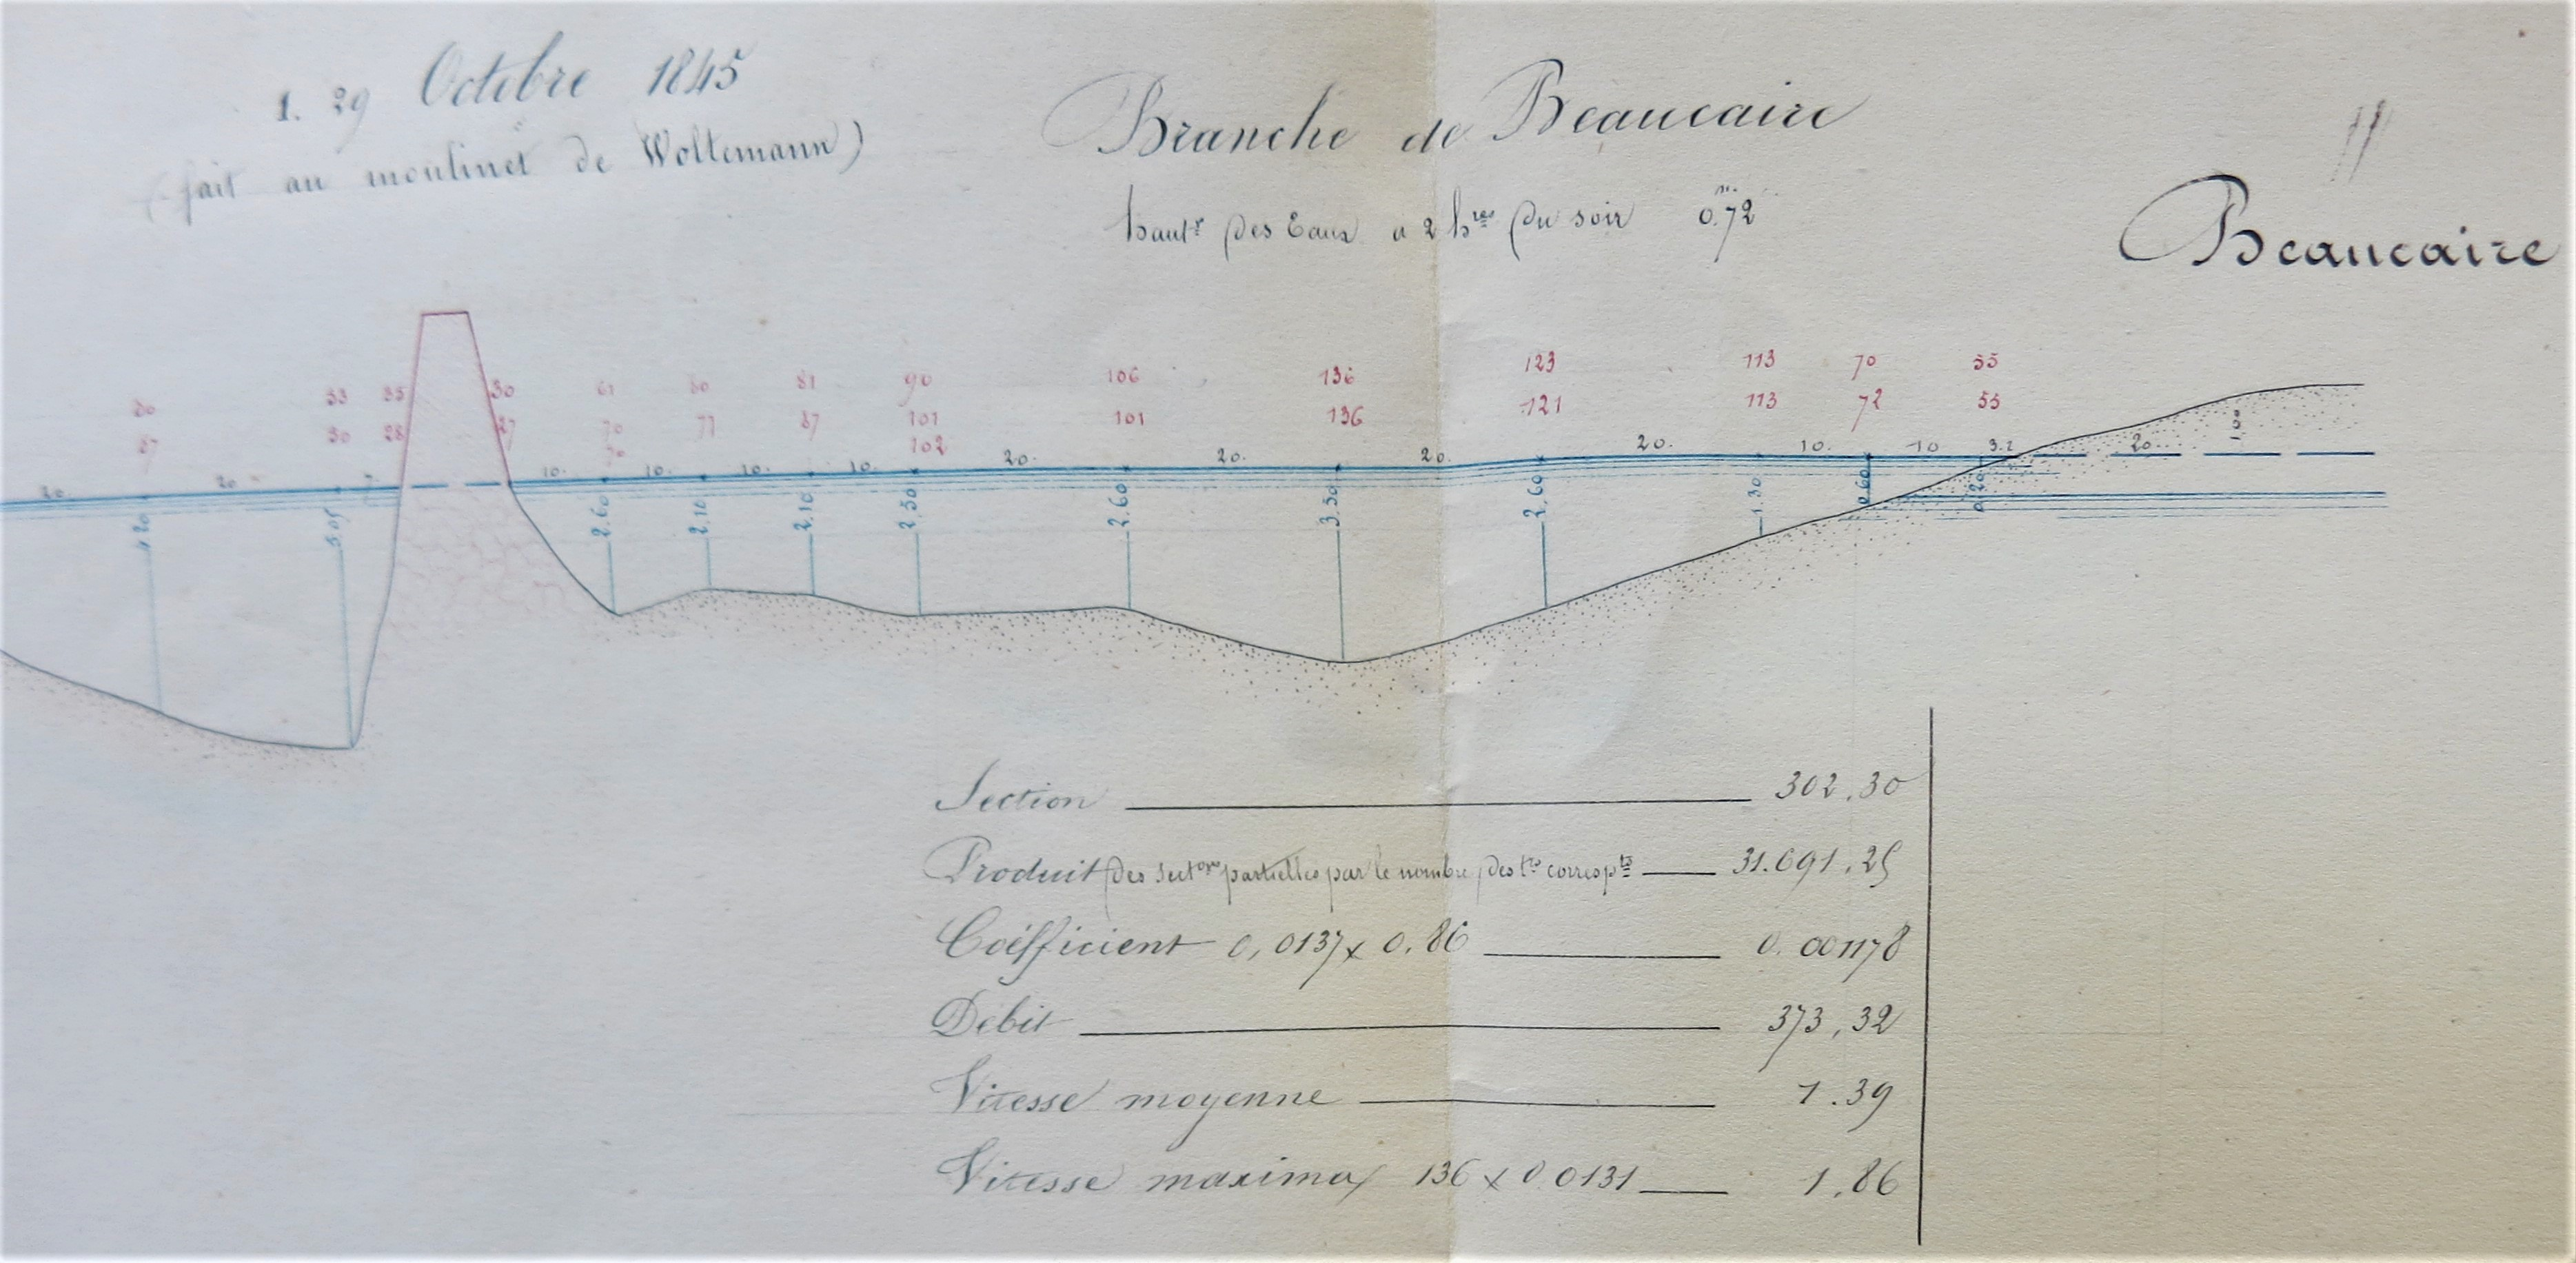
\includegraphics[width=.7\linewidth]{Chapitre2/Figures/Jau1845.jpg}
        \caption{Jaugeage du 29 octobre 1845 au droit de la station de Pont de Beaucaire, réalisé au moulinet de Woltmann par le Service Spécial du Rhône. En bas à droite, le détail du calcul du débit. Les chiffres en rouge représentent le nombre de tours du moulinet.}	
		\label{fig:Jau1845}
	\end{figure}
    	
    \begin{figure}[h]
	\centering
		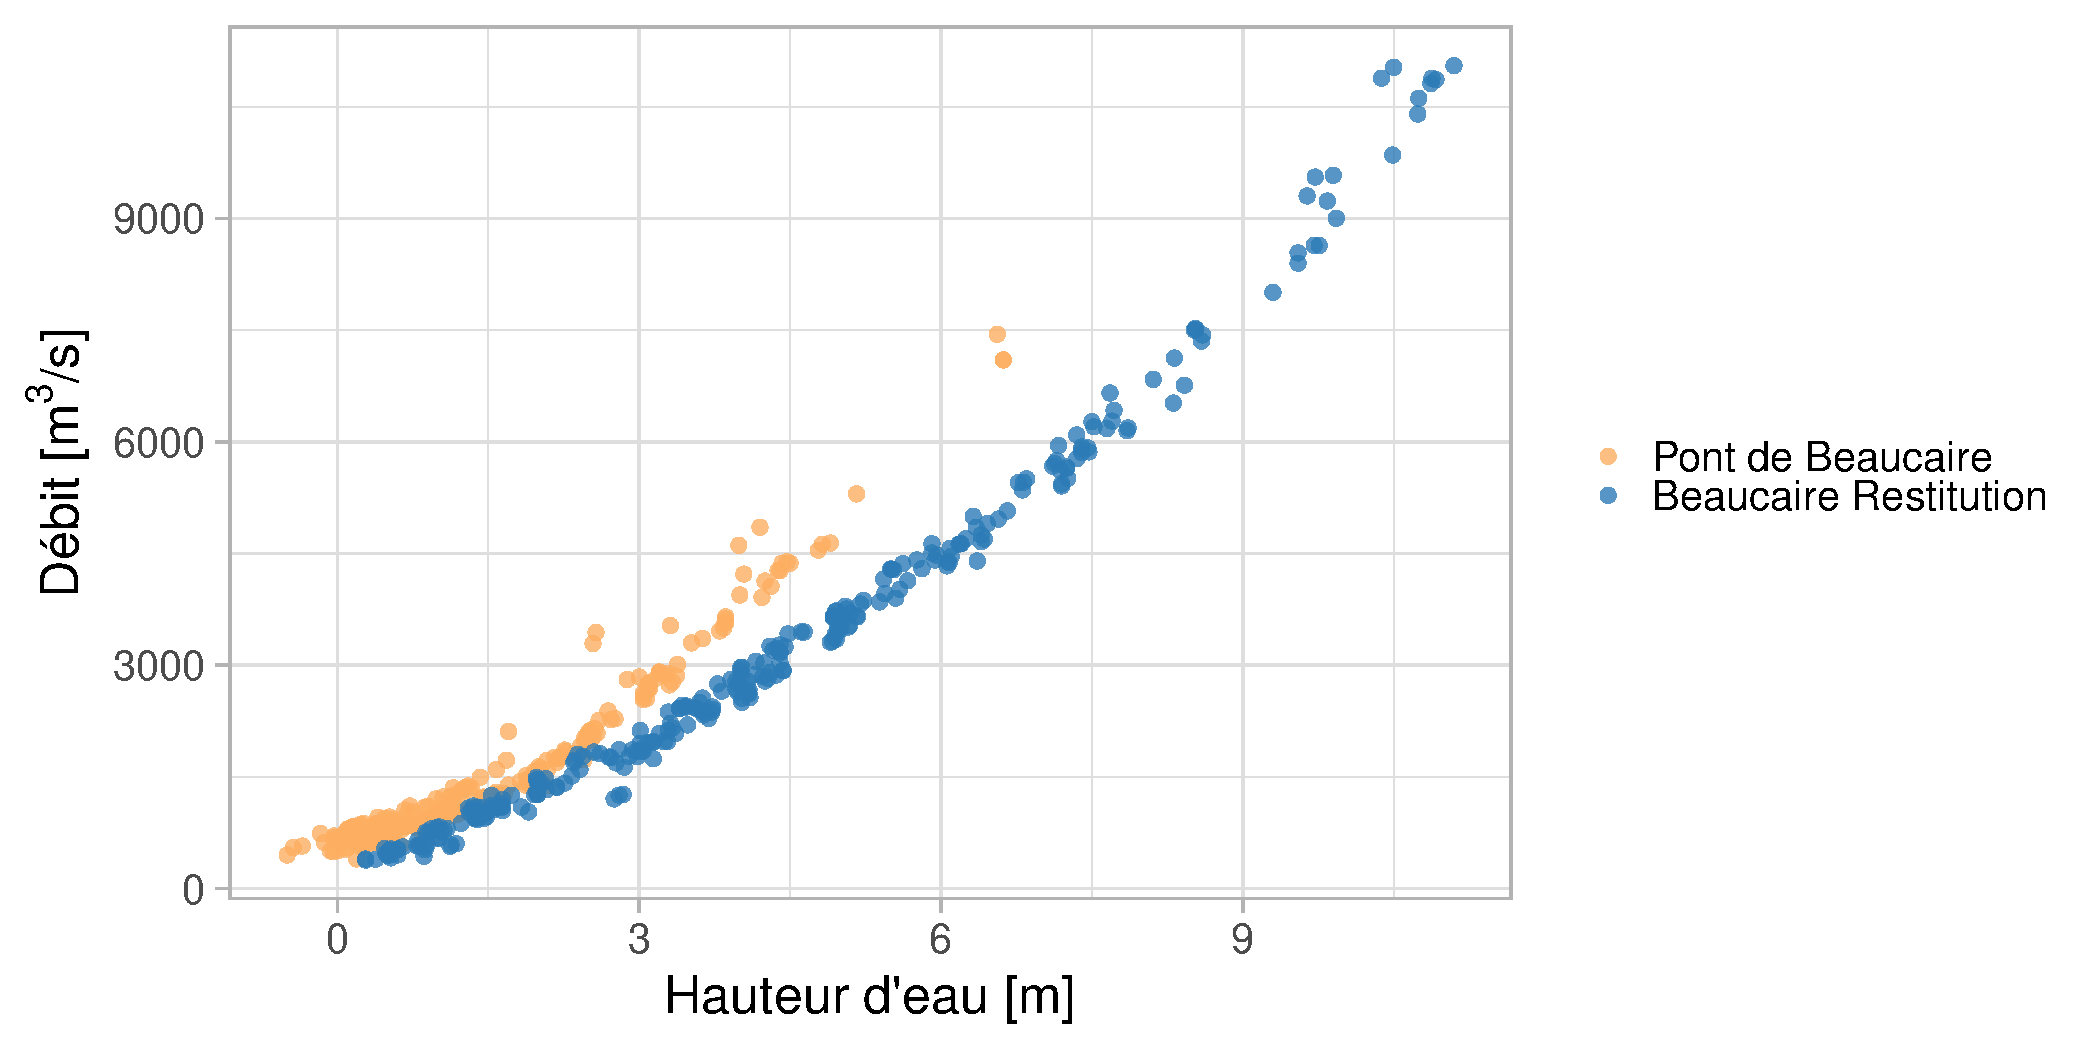
\includegraphics[width=.8\linewidth]{Chapitre2/Figures/Jaus.pdf}
        \caption{Jaugeages du Rhône à Pont de Beaucaire et Beaucaire Restitution de 1845 à 2020.}	
		\label{fig:JauAll}
	\end{figure}
   
\FloatBarrier

	\subsubsection{Évolution de l'altitude du zéro de l'échelle}
    
    \paragraph{} Comme attesté par \citet{pichard_hauteurs_2013}, l'échelle limnimétrique de Pont de Beaucaire possède le rare avantage d'être restée à la même place depuis 1816, avec une altitude du zéro relativement stable dans l'histoire de la station. Malgré divers changements de référentiels altimétriques au cours du temps, le zéro semble n'avoir que très peu varié (tableau \ref{tab:zeroPt}). De la même manière que \citet{bard_actualisation_2018}, nous retiendrons la dernière mesure de la CNR qui semble être une valeur médiane de l'ensemble des valeurs connues : 3.37~m~NGF~IGN69. De plus, celle-ci est compatible avec les valeurs données lorsque la station était encore exploitée.

            \begin{table}[h]
                \centering
                \caption{Mesures de l'altitude du zéro de l'échelle à Pont de Beaucaire}
            	\label{tab:zeroPt}
                \begin{tabular}{| m{1.5cm} | m{3cm}| m{3cm} | m{2cm} |} 
                    \hline
                    Date & Altitude du zéro [m NGF IGN69] & Organisme \\
                    \hline
                    1959 &	3.375 &	CNR\\
                    \hline
                    1961 &	3.36 &	CNR\\
                    \hline
                    2010 &	3.38 &	Symadrem\\
                    \hline
                    2010 &	3.37 &	CNR\\
                    \hline
            \end{tabular}
        \end{table}


\FloatBarrier

		\subsubsection{Travaux et aménagements}
    	\label{subsubsec:TravauxPt}
    
    \paragraph{} La largeur de la section du Rhône au niveau de Beaucaire (ou du moins, la largeur du lit majeur) n'a que peu évolué dans l'histoire car elle se situe au niveau d'un resserrement entre deux collines rocheuses. Ce resserrement est bien visible sur les champs d'inondation de 1840 et 1856 (Figure \ref{Champ1856}). En revanche, à une échelle plus réduite, de nombreuses modifications morphologiques, d'origine naturelle ou anthropique ont pu affecter l'écoulement et modifier la relation hauteur/débit durant les deux siècles de relevés limnimétriques. Ces évolutions sont décrites dans les paragraphes suivants.
        
    \begin{figure}[h]
        \centering
        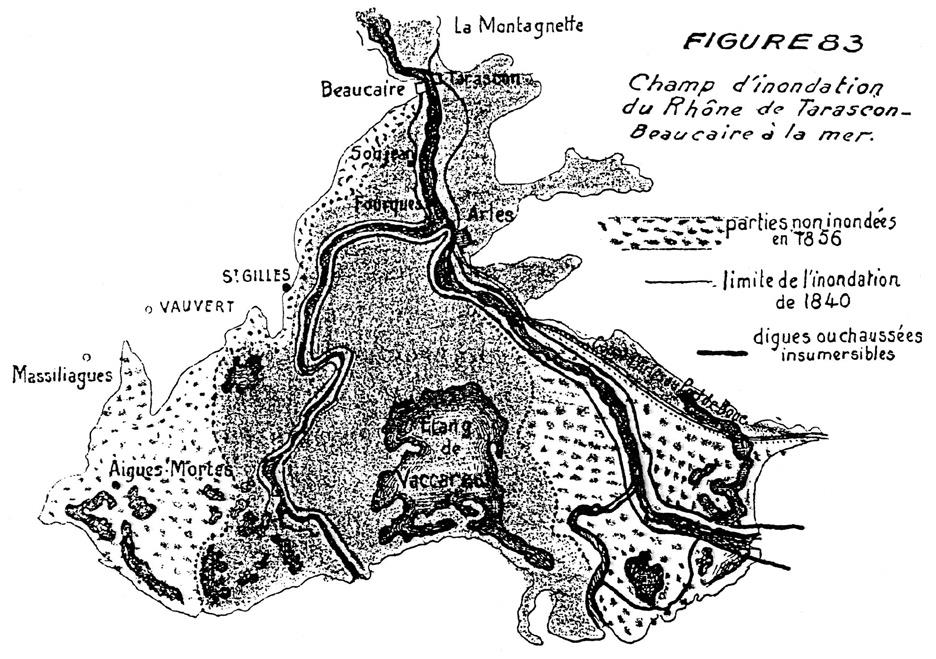
\includegraphics[width=.7\linewidth]{Chapitre2/Figures/ChampInond1840-1856.jpg}
        \caption{Champ d'inondation du Rhône aval lors des crues de 1840 et 1856, d'après \citet{parde_regime_1925}}
        \label{Champ1856}
    \end{figure}
    

	\paragraph{} Le premier pont reliant Beaucaire à Tarascon date de 1829. Il s'agit d'un pont suspendu composé de 4~piles (d'après la carte d'état-major de 1840), situé environ 30~m à l'amont du pont actuel, soit environ 45~m à l'amont de l'échelle limnimétrique. Quelques années plus tard, en juillet 1852, était inauguré le viaduc de chemin de fer de Beaucaire. Il est situé environ 250 m à l'aval de la station. Par la suite, les seuls travaux significatifs qui ont eu lieu dans le secteur sont ceux de l'aménagement CNR de Vallabrègues, entre 1967 et 1970. Ils ont sonné la fin de l'utilisation de la station par la CNR, la mesure n'étant plus représentative de la totalité du débit du Rhône suite à la création du canal de dérivation de l'aménagement. On peut noter la construction du pont routier actuel, entre 1988 et 1990, 30~m à l'amont de l'ancien pont. 
        

        \paragraph{} À Beaucaire, depuis l'époque des plus anciennes cartes et des plus anciens récits jusqu'à aujourd'hui, des bancs de sable et îlots de diverses formes et dimensions ont séparé l'écoulement en deux bras plus ou moins distincts selon les périodes. De tout temps, mais pour des hauteurs d'eau différentes, les deux bras ont communiqué, un bras prenant le dessus sur l'autre au gré des événements morphogènes. Petit à petit, ces îlots ont été fixés par des digues afin de faciliter la navigation dans la zone, pour finalement arriver à la situation actuelle de deux bras bien distincts, comme en témoigne la carte d'\citet{armand_ii_1907} (figure \ref{fig:DigArmand}) qui décrit les différentes étapes de cette séparation :
        
         \begin{figure}[h]
            \centering
            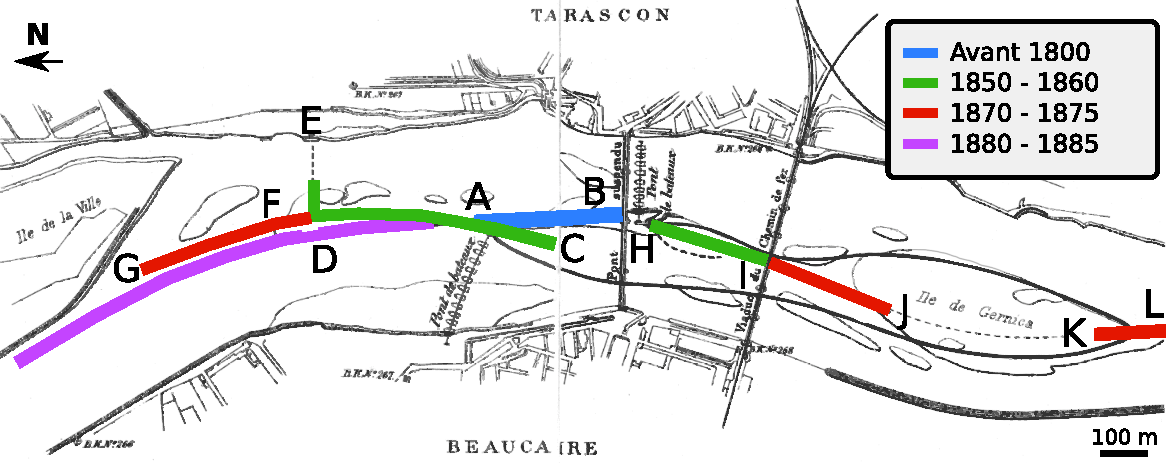
\includegraphics[width = 0.8\linewidth]{Chapitre2/Figures/EditArmand.pdf}
            \caption{Carte de l'historique des digues de Beaucaire, adaptée de \citet{armand_ii_1907}}
            \label{fig:DigArmand}
        \end{figure}
        
        \begin{itemize}
            \item[$\bullet$] Digue divisoire (\textbf{AB}), antérieure à 1782
            \item[$\bullet$] Atterrissement (trait plein noir sur la carte) qui, dès 1826 se prolongeait jusqu'au point aval de l'île de Gernica. Il était probablement déjà présent au début du 19ème siècle.
            \item[$\bullet$] Érosion de l'île de la ville (à l'amont de Beaucaire) qui a modifié la répartition des débits entre les deux bras en faveur du bras de Tarascon. Pour maintenir la navigation dans le bras de Beaucaire, la digue \textbf{AB} fut prolongée à l'amont par une digue concave \textbf{CDF} en 1851 et par la suite, obstruction partielle du bras de Tarascon entre 1852 et 1855 \textbf{DE}. On peut constater cette érosion très rapide en faveur du bras de Tarascon sur les profils en travers de Goux (1850) (Figure \ref{fig:ProfGoux}). L'érosion de l'île de la ville peut être attribuée notamment à la crue catastrophique de 1840, possible déclencheur de ce phénomène.
            \item[$\bullet$] Forte érosion de l'atterrissement au niveau de \textbf{HI} du fait de l'écart de hauteur d'eau entre les deux bras pendant les crues. Une digue fut construite entre 1858 et 1859 pour pallier ce phénomène.
            \item[$\bullet$] Pour ces mêmes raisons, construction d'une digue en aval du viaduc de chemin de fer \textbf{IJ} en 1872-1875 ainsi que la digue \textbf{KL} à l'aval de l'île de Gernica, qui se prolonge actuellement sur 2 km vers l'aval.
            \item[$\bullet$] Prolongement de la digue concave \textbf{GF} autour de 1875
            \item[$\bullet$] Construction d'une nouvelle digue concave à l'amont de \textbf{GF} entre 1880 et 1884
        \end{itemize}

        \begin{figure}[h]
            \centering
            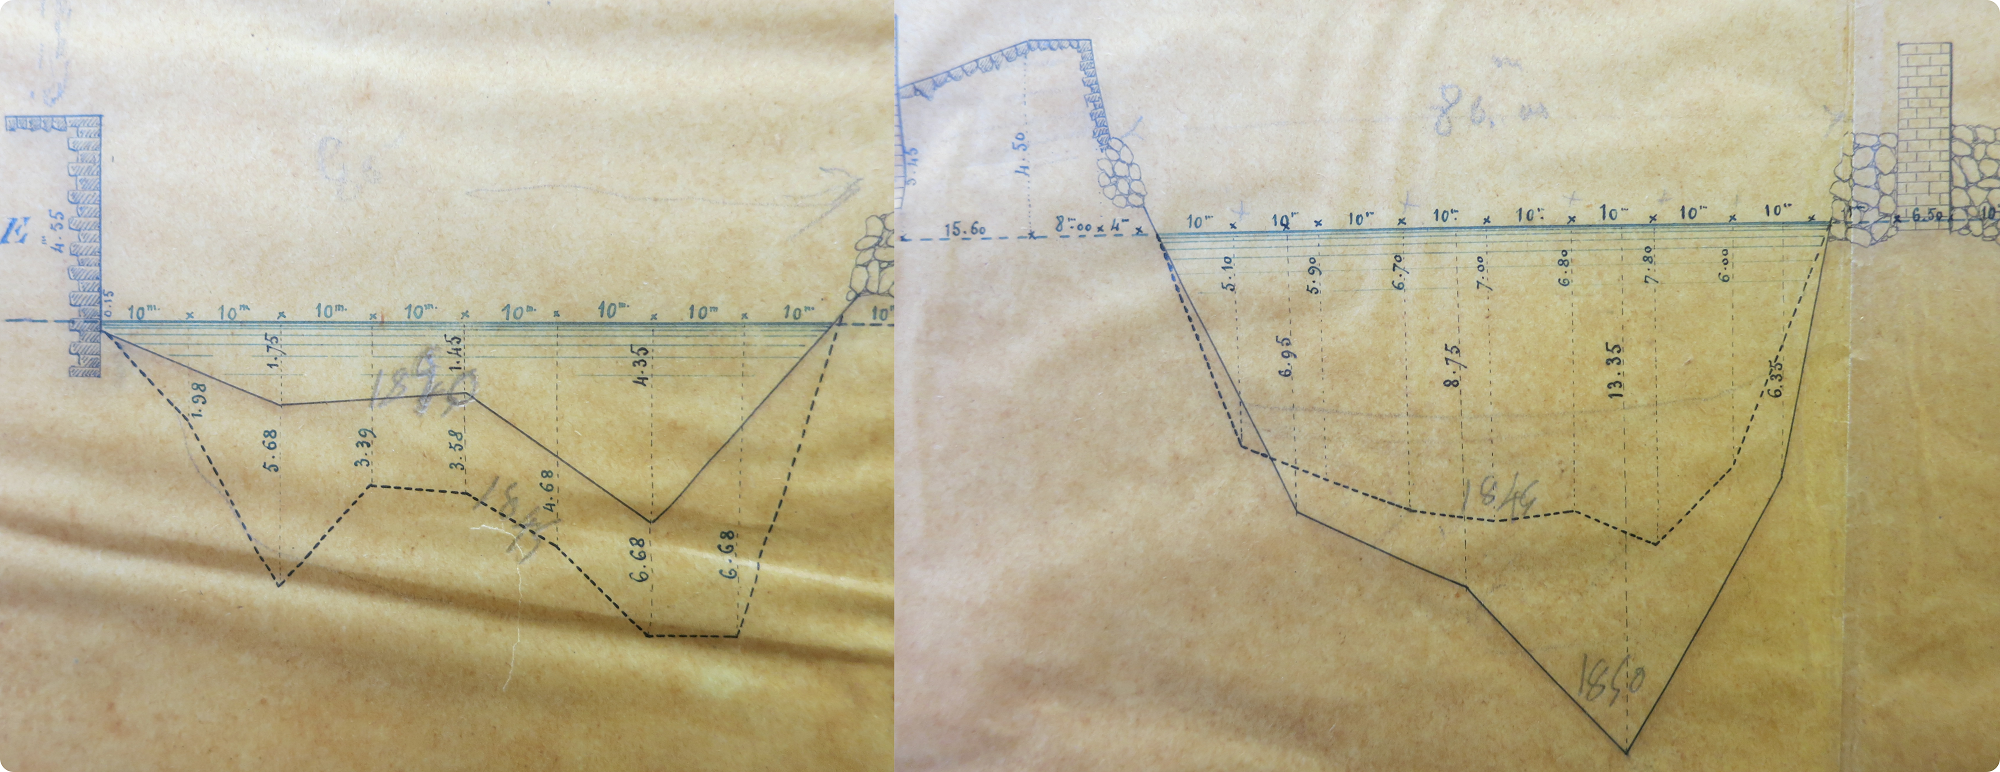
\includegraphics[width = 0.9\linewidth]{Chapitre2/Figures/Goux4550.png}
            \caption{Portions de profil en travers au niveau du pont suspendu de Beaucaire. Il s'agit des bras de Beaucaire (gauche) et Tarascon (droite), en 1845 (pointillés) et 1850 (trait continu) \citep{goux_modification_1851}. On constate l'approfondissement du bras de Tarascon et le comblement du bras de Beaucaire.}
            \label{fig:ProfGoux}
        \end{figure}
%            
%        \begin{figure}[h]
%            \centering
%            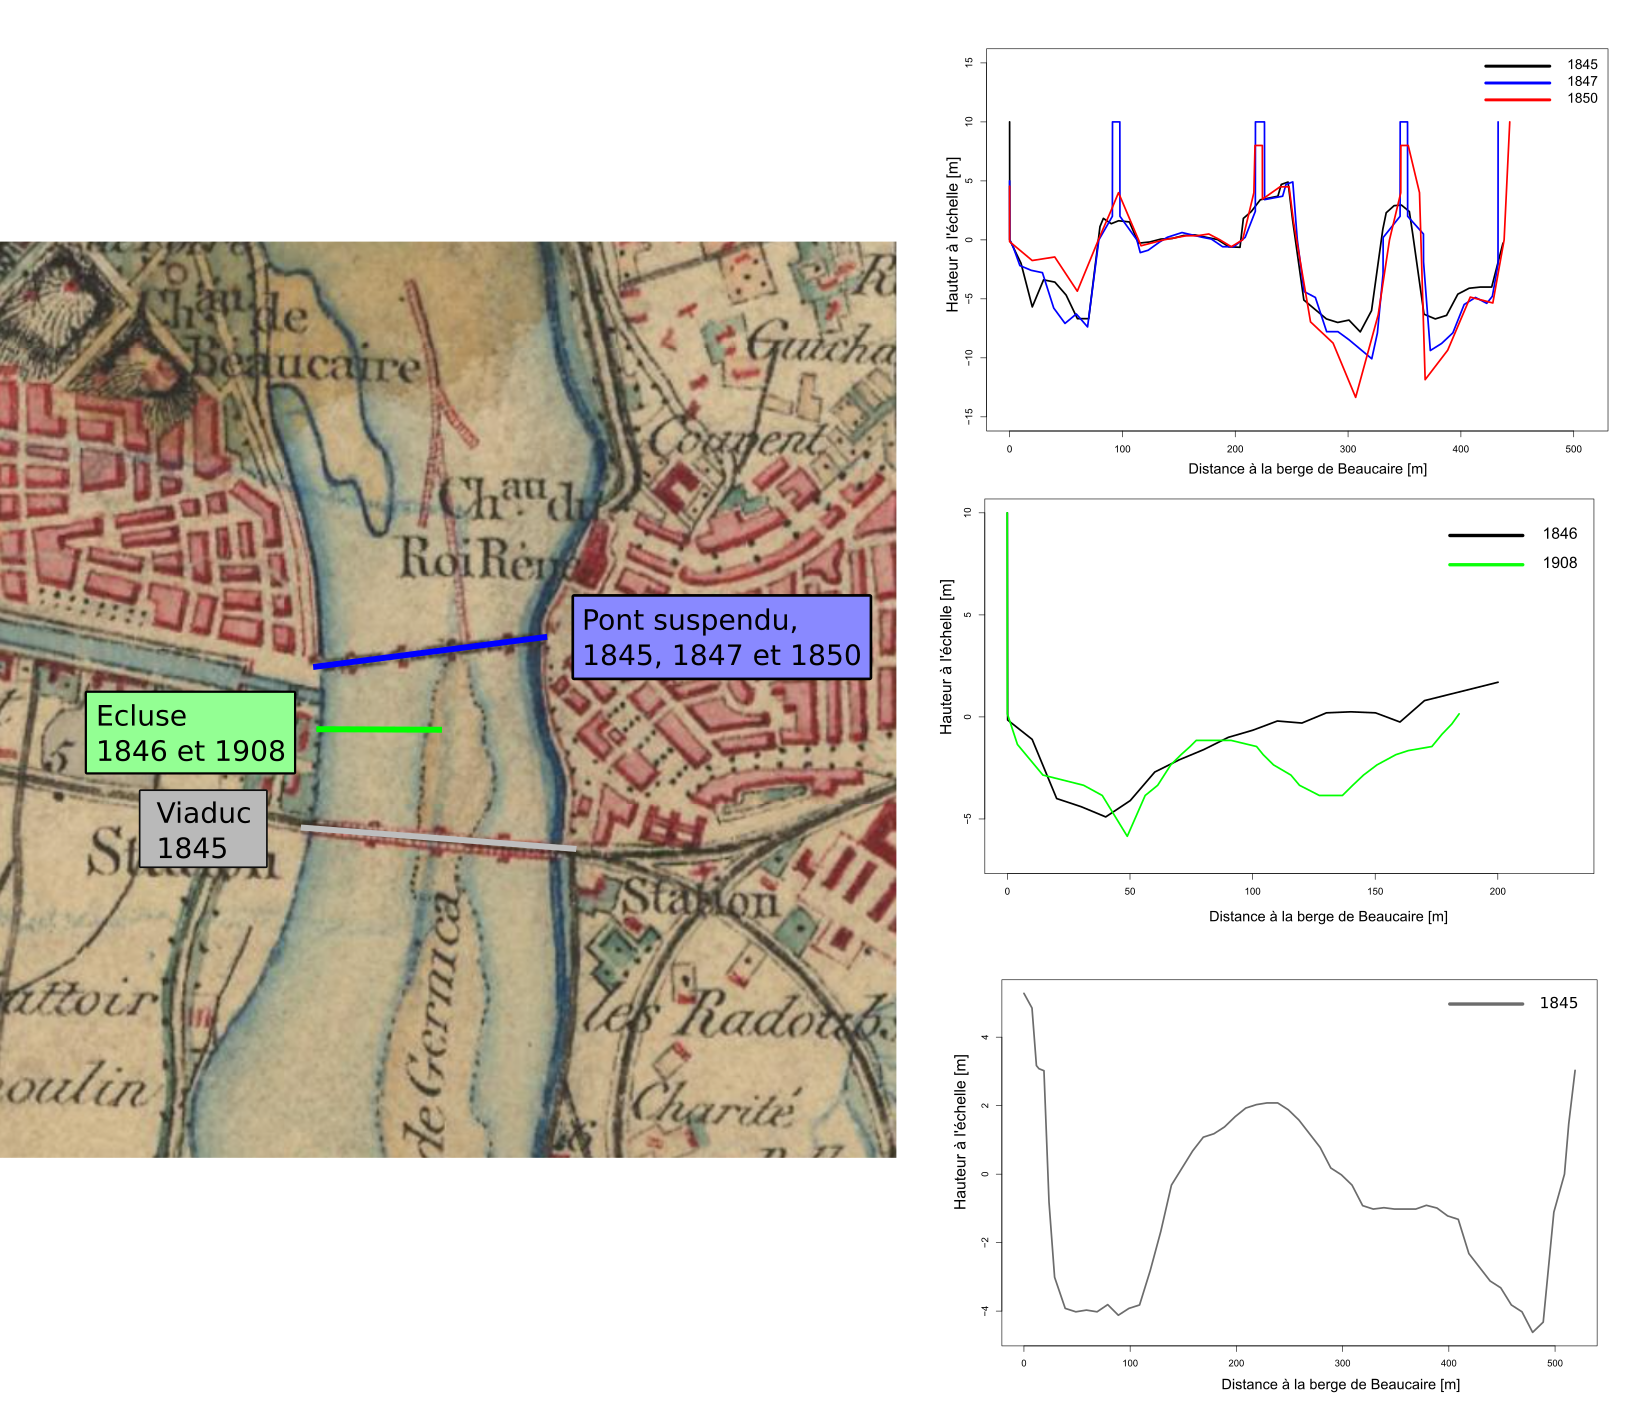
\includegraphics[width = 0.7\linewidth]{Chapitre2/Figures/MapProfils.png}
%            \caption{Profils en travers du lit mineur du Rhône à Beaucaire au XIXème siècle}
%            \label{fig:Profils19eme}
%        \end{figure}
            
\FloatBarrier
        \paragraph{} Suite à la fixation des deux bras par les digues divisoires vers la fin du XIX\textsuperscript{ème} siècle, on peut supposer qu'il n'y a eu pratiquement aucun changement jusqu'au début des aménagements CNR de Vallabrègues (débutés en 1967 et mis en service en 1970), comme en témoignent les photos aériennes du portail "Remonter le temps" de l'IGN, de 1936 à 1947 (Figure \ref{fig:AerialBcr}). Ainsi, l'isolement quasi-total du bras de Tarascon au profit du bras de Beaucaire est finalisé en 1884 et a connu de nombreuses phases d'aménagement débutant vers la fin du 18\textsuperscript{ème} siècle. Il est probable qu'à l'époque ancienne, tout comme aujourd'hui, les deux bras communiquaient à haut débit, certainement aux alentours de 6 m à l'échelle à l'époque de la finalisation des digues, et à des hauteurs moindres auparavant. Certaines sources signalent par exemple qu'il était ponctuellement possible de traverser en bateau d'un bras à l'autre au niveau de la ville entre 1858 et 1872. Le bras de Beaucaire a sans doute été prépondérant sur le bras de Tarascon sur la majeure partie de l'histoire de la station, excepté durant la période 1840-1850, comme en témoignent les profils en travers de \citet{goux_modification_1851} (figure \ref{fig:ProfGoux}).
    
        \begin{figure}[h]
            \centering
        	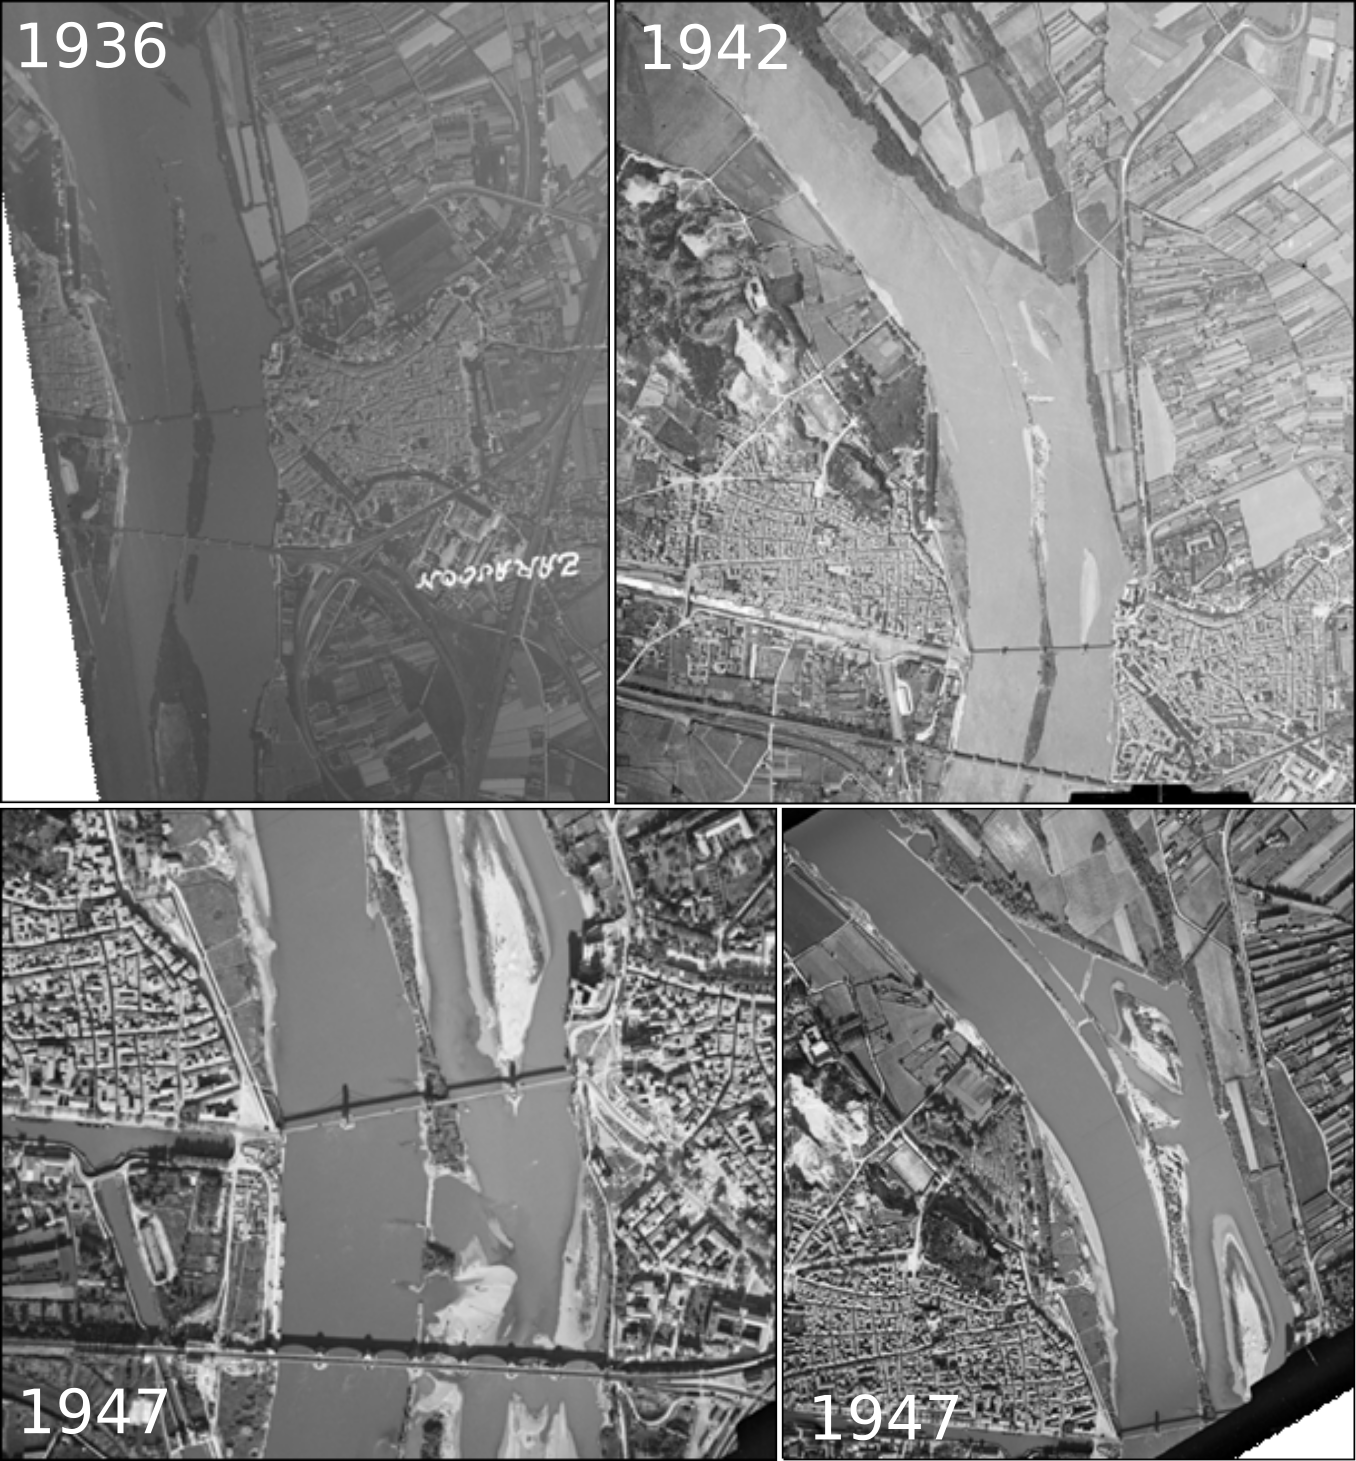
\includegraphics[width = 0.7\linewidth]{Chapitre2/Figures/AerialBcr.png}
            \caption{Images aériennes du Rhône à Beaucaire entre 1936 et 1947 (source : www.géoportail.gouv.fr). On remarque la présence des digues sur les 4 images, particulièrement en 1947 pour des débits très faibles.}
            \label{fig:AerialBcr}
        \end{figure}
    
		\paragraph{} Au cours des décennies 1860 et 1870, les travaux d'aménagement en lit mineur imaginés par l'ingénieur Girardon sont lancés. Ils permettront de favoriser la navigation fluviale en fixant les berges par l'installation d'épis noyés transversaux sur une grande partie du linéaire du Rhône français. Des épis ont été installés à l'amont et à l'aval de Beaucaire et ont probablement influencé la relation hauteur/débit au droit de la station.
    
		\paragraph{} Les désordres du Rhône à l'aval de Beaucaire étant réguliers avant son endiguement, on imagine que la création des digues a coïncidé avec l'installation des populations dans le secteur, comme attesté par \citet{surell_memoire_1847} : «\textit{Si l'on considère que l'existence de la plaine est presque inévitablement liée à celle des chaussées, on doit croire que celles-ci sont contemporaines de la civilisation même du pays, et qu'elles ont dû occuper, depuis longtemps, les soins de la population}» (les digues étaient fréquemment appelées chaussées dans l'époque ancienne, car elles faisaient également office de voies de circulation). \citet{mejean_etude_2017}, cite l'ingénieur Girard, qui, en 1857, affirme que : «\textit{la construction des premières chaussées entre Beaucaire et Sylvéréal (Camargue) date de l'époque romaine. L'initiative personnelle des propriétaires a ensuite contribué à dresser un système de protection où chacun établissait une levée de terre pour se protéger des invasions du Rhône. La plupart de ces chaussées étaient établies sur les bourrelets alluviaux, car ils présentaient l'avantage d'être déjà surélevés par rapport aux terres voisines. Les chaussées ne présentaient pas une ligne continue de défense, les protections s'établissant autour de quelques grandes propriétés.}» Par la suite, plusieurs grandes phases d'aménagement des digues de protection se sont succédées. Avant le XVI\textsuperscript{ème} siècle, les aménagements étaient discontinus mais deviennent plus organisés avec l'essor de l'agriculture dans les plaines alluviales. Au début du XIX\textsuperscript{ème} siècle, un endiguement continu de Beaucaire à la mer est installé grâce à l'harmonisation des nombreuses associations ou "syndicats des digues", jusqu'alors «\textit{aussi multiples que rivales}» \citep{pichard_sept_2014}. Cet endiguement protège les populations pour les crues courantes et jusqu'à la décennale. Au niveau de Beaucaire, la digue de la Montagnette existant depuis le XV\textsuperscript{ème} siècle connut de nombreuses avaries en 1840, 1841, 1843. Des travaux de rehaussement furent effectués en 1843 ainsi qu'en 1883. La digue du chemin de fer (de Tarascon à Arles en rive gauche) vint remplacer en 1846 les digues historiques du Trébon, souvent rompues dans l'histoire. La digue du Trébon était élevée à 6.5 ou 7 m au-dessus de l'étiage. La digue du chemin de fer est élevée à 2.10 m au-dessus des plus hautes eaux connues à l'époque (1843). Lors de la rupture de la digue de la Montagnette en 1856, Tarascon était enfermée entre Montagnette et le remblai du chemin de fer, l'eau était ainsi restée dans les plaines pendant plusieurs semaines. Ces digues principales furent complétées par des aménagement au sein des villes de Tarascon et Beaucaire entre 1860 et 1866. La "banquette de Beaucaire", constituée d'un mur maçonné construit en 1840 du rocher du château à la chaussée du chemin de fer, fut rehaussée après 1856, puis en 1862 et 1863, environ 2 m au-dessus du niveau atteint en 1856. Il en va de même pour les quais de Tarascon et de la digue de la Montagnette, rehaussés en 1860 à 1.5 m au-dessus du niveau de 1856.
		
	\paragraph{} Ces nombreuses protections érigées au cours du XIX\textsuperscript{ème} siècle ont permis de contenir les crues courantes, puis des crues plus importantes grâce aux aménagements postérieurs aux inondations de 1840 et 1856 qui furent à l'origine d'une prise de conscience illustrée par la création du Service Spécial du Rhône par les Ponts et Chaussées. Depuis cette époque, les systèmes de protection n'ont que peu évolué et la crue de 2003 a ravivé les inquiétudes quant au risque de brèches, comme en témoigne cet extrait du rapport du \citet{symadrem_programme_2012} (Syndicat Mixte Interrégional d'Aménagement des Digues du Delta du Rhône et de la Mer) : «\textit{Le système actuel de protection contre les crues du Rhône a été réalisé après les grandes crues de 1840 et 1856. Il est ancien et présente une exposition très forte au risque de brèches. Dans l'état actuel, on estime que que le risque de formation de brèches, confirmé par les crues de 1993, 1994, 2002 et 2003, est quasi-certain à certain}». Depuis la crue de 2003, un programme de sécurisation a été réalisé, prévoyant notamment la réalisation de digues résistantes à la surverse et à la formation de brèches \citep{symadrem_programme_2012}.    
		

\FloatBarrier
	\subsection{Station hydrométrique du Rhône à Beaucaire Restitution (1970-aujourd'hui)}
	\label{subsec:Restit}
	\subsubsection{Données disponibles}

	\paragraph{} La station de Beaucaire Restitution (PK 269.6) a pris le relais sur la station de Pont de Beaucaire suite aux travaux de l'aménagement hydroélectrique de Vallabrègues, et de l'installation d'un chenal de dérivation restituant une partie du débit à l'aval de la ville de Beaucaire. La nouvelle station fut alors installée 2 km plus à l'aval, environ 600 m à l'aval de la restitution des débits transitant par la centrale hydroélectrique CNR de façon à mesurer la totalité du débit (figure \ref{fig:CartoRes}). Durant les travaux, de 1967 à 1970, les débits de la Durance ayant été dérivés vers l'étang de Berre, les relevés des deux stations sont considérés comme manquants. La station de Beaucaire Restitution demeure au même emplacement depuis sa mise en service en 1970. Elle est équipée dès sa création de capteurs automatiques réalisant des relevés au pas de temps infra-horaire. L'ensemble de ces relevés, ainsi que les jaugeages réalisés à la station, sont disponibles au sein des bases de données de la CNR.
		
	\begin{figure}[h]
	\centering
		\includegraphics[width=.9\linewidth]{Chapitre2/Figures/RestitCartoPh.png}
        \caption{Gauche : Localisation de la station de Beaucaire Restitution (carte IGN Scan25, source : \url{www.geoportail.fr}). Droite : échelle limnimétrique de Beaucaire Restitution en février 2020.}	
		\label{fig:CartoRes}
	\end{figure}
	
	
		\subsubsection{Travaux et aménagements}

	\paragraph{} La section du Rhône au niveau de la station de Beaucaire Restitution a connu de nombreux dragages des matériaux du fond du lit suite à la construction de l'aménagement de Vallabrègues, durant les 5 années après la mise en service du système en 1970, ainsi qu'entre 1998 et 2000, pendant la construction du nouveau pont routier reliant Tarascon à Beaucaire. En dehors de ces interventions, le profil au droit de la station est stable, comme en témoignent les profils en travers du lit mineur au droit de la station (figure \ref{fig:ProfilsRestit}).
	
	\begin{figure}[h]
	\centering
		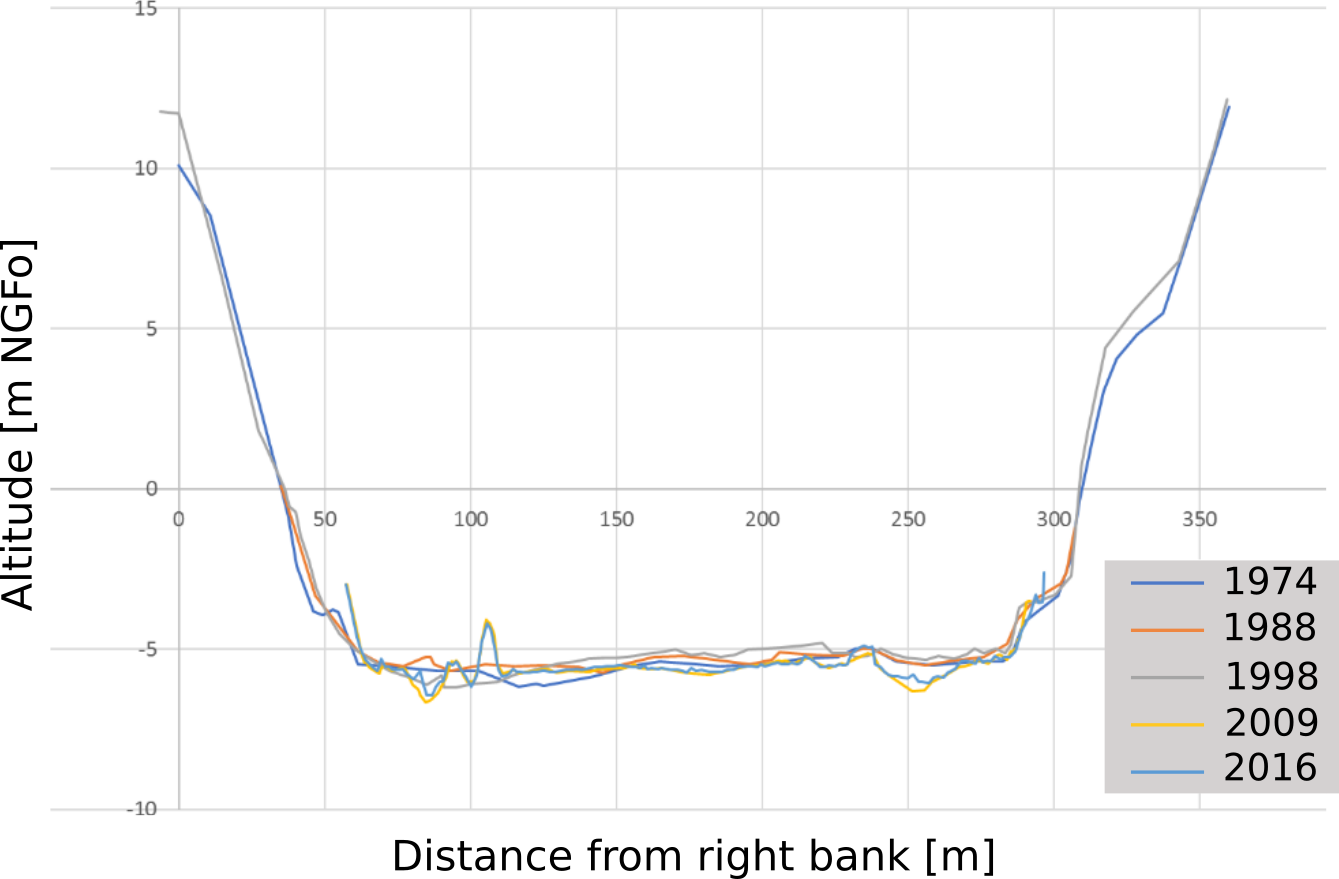
\includegraphics[width=.6\linewidth]{Chapitre2/Figures/ProfilsBardRestit.png}
        \caption{Profils en travers du Rhône à la station de Beaucaire Restitution réalisés par la CNR entre 1974 et 2016. Adapté de \citet{bard_actualisation_2018}. À Beaucaire, on passe de l'altitude NGF ortho (ou Lallemand) à l'altitude NGF IGN69 en ajoutant 3 cm.}	
		\label{fig:ProfilsRestit}
	\end{figure}
	
\FloatBarrier


\subsection{Évolution du temps de propagation des crues}

	\paragraph{} Les aménagements en lit mineur du Rhône français, débutés dès la seconde moitié du XIX\textsuperscript{ème} siècle, ont eu des conséquences directes sur la géométrie du chenal. Rapidement, la largeur du lit mineur et la ligne d'eau ont été impactées (\cite{gaydou_schema_2013}; \cite{piegay_observatoire_2022}). Une conséquence de ces aménagements pourrait être la modification de la dynamique d'écoulement des crues sur le continuum fluvial. On peut en effet se demander si la transition d'un style fluvial naturel et complexe vers un chenal unique et quasiment rectiligne (figure \ref{fig:CartesChenal}) n'aurait pas eu pour conséquence de modifier la vitesse de propagation des événements de crue, et d'impacter le laminage des crues le long de la moyenne et basse vallée du Rhône. Ces modifications morphologiques pouvant impacter la stationnarité des débits, et donc l'analyse fréquentielle des crues, leurs conséquences sont étudiées dans cette section.
	
	\begin{figure}[h]
		\centering
		\begin{subfigure}{0.49\linewidth}
			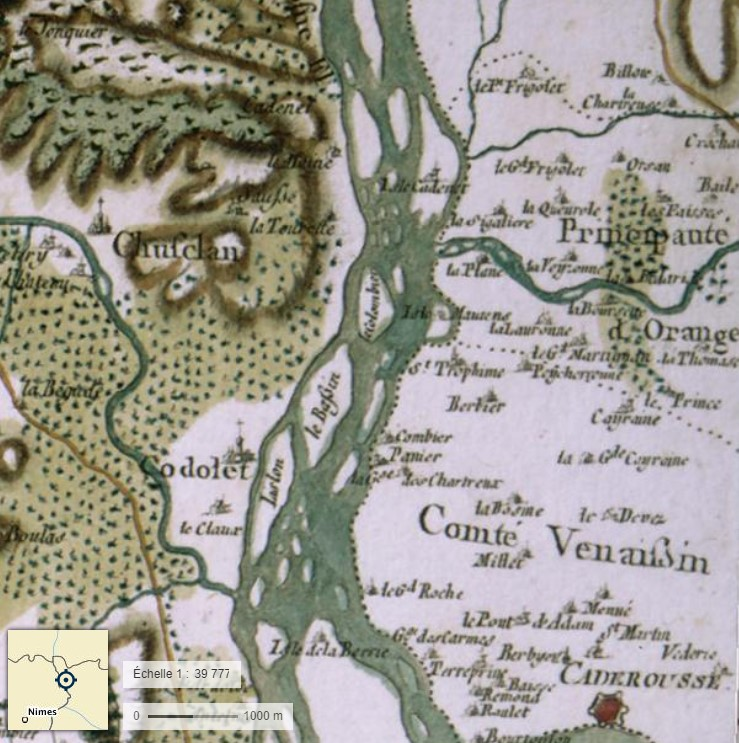
\includegraphics[width=\linewidth]{Chapitre2/Figures/CassiniOrange.jpg}
		\end{subfigure}
		\begin{subfigure}{0.49\linewidth}
			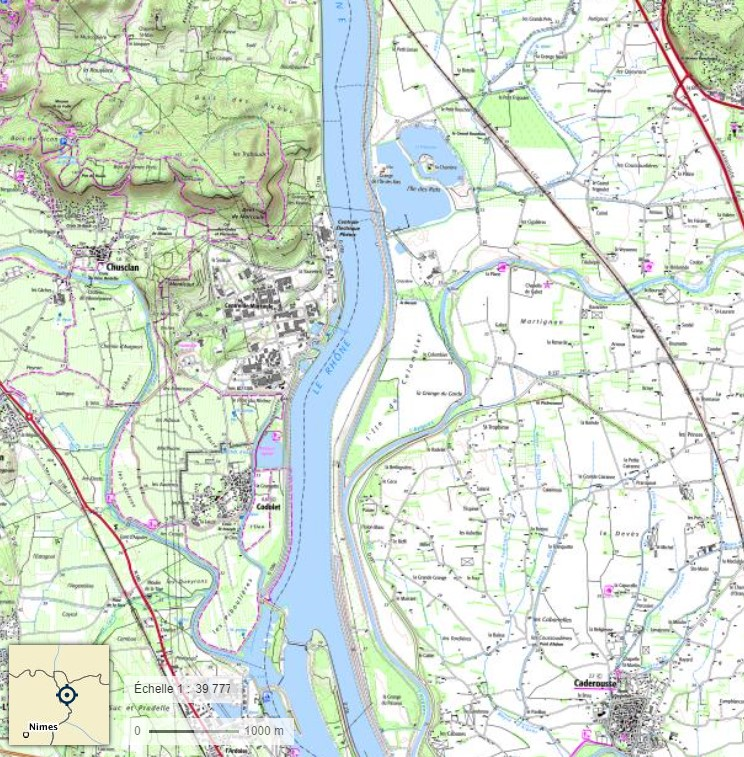
\includegraphics[width=\linewidth]{Chapitre2/Figures/IGNOrange.jpg}
		\end{subfigure}
		\caption{Cartes du Rhône au niveau de la ville d'Orange (environ 50 km à l'amont de Beaucaire). A gauche, la carte de Cassini datant du XVIII\textsuperscript{ème} siècle présente un chenal en tresses. A droite, la carte IGN actuelle présente un chenal unique et contraint. (source : \url{geoportail.gouv.fr})}
		\label{fig:CartesChenal}
	\end{figure}
	
	\paragraph{} Dans le but d'étudier l'impact au cours du temps des aménagements en lit mineur sur le temps de propagation des crues, il est possible d'analyser le délai entre le passage du pic de crue à l'amont et à l'aval du linéaire aménagé. «\textit{Les aménagements Girardon […] conçus et mis en place entre 1880 et 1920 […] sont présents depuis le pont de Rochefort en amont [environ 80 km à l'aval du lac Léman], jusqu'à la mer. Ils sont moins nombreux en amont de Lyon, où ils se limitent à une digue longitudinale basse et des épis}» \citep{gaydou_schema_2013}. Suite à ce constat, il est décidé de limiter l'analyse au linéaire entre Lyon et Beaucaire, considérant que les aménagements présents à l'amont de Lyon, par leur forme différente et leur moindre présence, n'ont eu que peu d'influence sur la dynamique des crues à Beaucaire.
	
	\paragraph{} Les aménagements en lit mineur du Rhône ont été conduits en plusieurs phases au cours des deux derniers siècles. Tout d'abord, la construction des premières digues pour l'amélioration de la navigation au milieu du XIX\textsuperscript{ème} siècle (section \ref{subsubsec:TravauxPt}). Ensuite, des travaux de plus grande ampleur organisés par l'ingénieur Girardon ont été réalisés sur l'ensemble du linéaire français entre 1880 et 1920. Ces travaux consistent notamment en l'installation d'épis et de casiers immergés qui concentrent l'écoulement vers le centre du chenal (figure \ref{subfig:Girardon}). Ce n'est ensuite qu'à partir de 1948 que de nouveaux travaux sont réalisés. Il s'agit de l'installation de 18 ouvrages hydroélectriques effectuée par la CNR sur l'ensemble du cours du Rhône français jusqu'en 1989. Ces aménagements sont pour la plupart construits sur un même schéma, à savoir l'installation d'un canal de dérivation qui court-circuite le chenal originel du Rhône, alors appelé "Vieux-Rhône" (figure \ref{subfig:SchemaCNR}). Ce sont donc trois grandes phases d'aménagement qui ont eu lieu depuis le début du XIX\textsuperscript{ème} siècle et qui ont indéniablement eu des conséquences sur la dynamique des écoulements. 
	
	\begin{figure}[h!]
		\centering
		\begin{subfigure}{0.8\linewidth}
		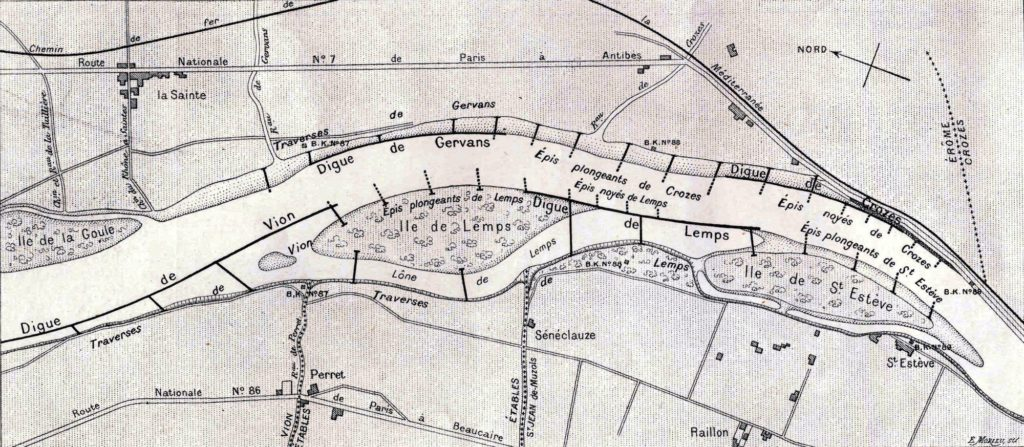
\includegraphics[width=\linewidth]{Chapitre2/Figures/EpisGirardonGervans.jpg}
		\caption{}
		\label{subfig:Girardon}
		\end{subfigure}	
		\begin{subfigure}{0.6\linewidth}
		\centering
		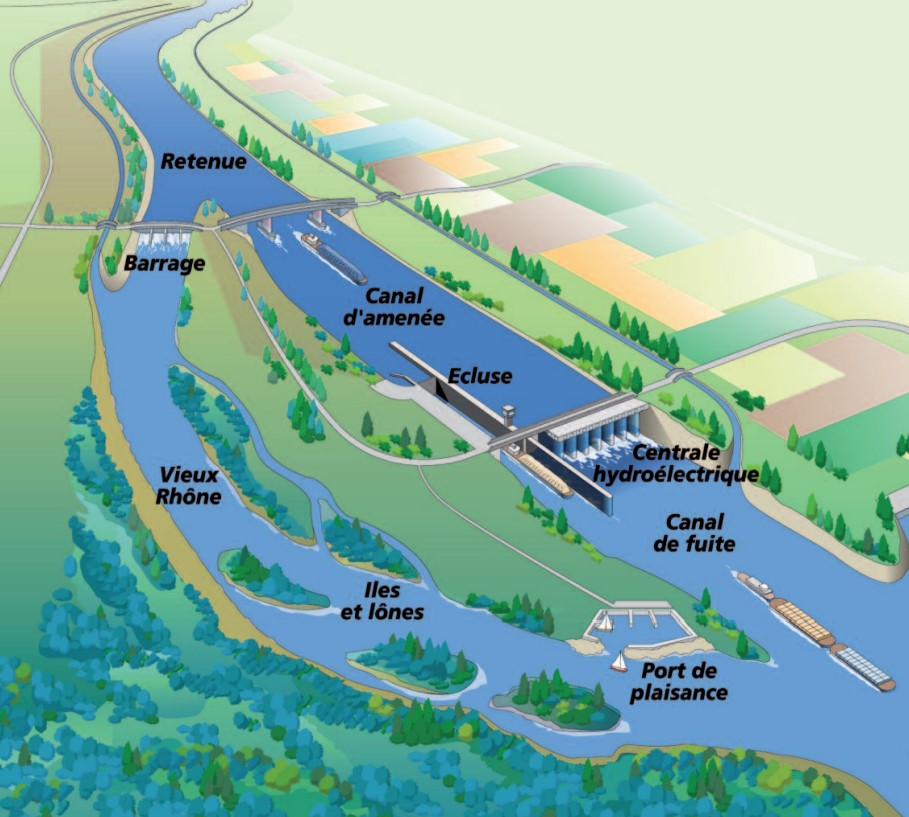
\includegraphics[width=\linewidth]{Chapitre2/Figures/AmenTypeCNR.jpg}
		\caption{}
		\label{subfig:SchemaCNR}
		\end{subfigure}
		\caption{(a) Carte des épis et casiers Girardon installés sur le Rhône au niveau de la commune de Gervans (environ 150 km à l'amont de Beaucaire). L'objectif est de concentrer l'écoulement dans le chenal principal et de le déconnecter des chenaux secondaires ou "lônes" (source : \url{www.capsurlerhone.fr}). (b) Schéma type d'un aménagement hydroélectrique du Rhône (source : CNR).}
	\end{figure}		

	\FloatBarrier
		
	\subsubsection{Sélection d'événements de crue}
	
	\paragraph{} Pour étudier le temps de propagation des crues entre Lyon et Beaucaire, il faut tout d'abord isoler les événements qui proviennent de l'amont de Lyon. Afin de faciliter l'identification de la pointe de crue à l'aval de la zone, il est préférable qu'aucun affluent entre Lyon et la mer ne soit lui aussi en crue. Ces conditions sont réunies pour les crues océaniques décrites par \citet{parde_regime_1919} : «\textit{Les crues océaniques du Bas Rhône sont dues à un double ou même à un triple flot : celui de l'Isère, celui du Rhône supérieur, celui de la Saône. Le flot de l'Isère est ordinairement négligeable en comparaison des deux autres}». Ce type de crue est associé à des événements pluvieux qualifiés eux aussi du titre "océanique" et qui surviennent généralement durant la saison automnale ou hivernale \citep{parde_regime_1925}. Lors d'événements de crue de magnitude importante, les échanges entre les écoulements du lit mineur et ceux du lit majeur ont un impact sur la dynamique de la crue. Afin de faciliter l'analyse du déplacement de l'onde de crue, les événements non-débordants sont privilégiés. Cette analyse se limitera donc au temps de propagation des crues océaniques dont le débit à Lyon est inférieur au débit de période de retour de 20 ans, et dont l'identification à Beaucaire n'est pas biaisée par des crues des affluents intermédiaires. 
	
	\paragraph{} Les données limnimétriques disponibles à Beaucaire décrites dans les sections précédentes consistent en des enregistrements continus de la hauteur d'eau depuis 1816, au pas de temps journalier (une mesure par jour à midi) jusqu'en 1885, puis trois mesures par jour jusqu'en 1967. A partir de 1970, les mesures sont automatisées et effectuées a minima toutes les heures. Pour la partie amont de la zone d'étude, la première station à l'aval de la confluence avec la Saône a été choisie. Il s'agit de la station située à Ternay, à une quinzaine de kilomètres à l'aval de Lyon. Celle-ci était à l'origine installée à la Mulatière, quelques kilomètres à l'amont de Ternay, où des relevés journaliers (une mesure par jour à midi) existent au moins à partir de 1840. La station a par la suite été déplacée de nombreuses fois comme décrit dans le tableau \ref{tab:Hternay}. Une lacune existe autour de la seconde guerre mondiale, entre 1935 et 1949. 
	
	\begin{table}[h]
	\centering
	\caption{Bilan des relevés limnimétriques disponibles aux stations de Ternay, Givors et La Mulatière.}
	\label{tab:Hternay}
%	\resizebox{\textwidth}{!}{%
		\begin{tabular}{|l|l|l|}
			\hline
			Station      & Période   & Pas de temps \\ \hline
			La Mulatière & 1840-1890 & 1/jour       \\ \hline
			Givors       & 1890-1910 & 1/jour       \\ \hline
			Givors       & 1910-1935 & 3/jour       \\ \hline
			La Mulatière & 1949-1966 & horaire      \\ \hline
			Givors       & 1966-1980 & horaire      \\ \hline
			Ternay       & 1982-2020 & horaire      \\ \hline
		\end{tabular}
%	}
	\end{table}

	
	\paragraph{} Ainsi, la période durant laquelle des relevés sont disponibles à l'amont et à l'aval de la zone d'étude s'étend de 1840 à aujourd'hui. Durant cette période, la fréquence des mesures évolue à la fois à l'amont et à l'aval pour finalement tendre vers des relevés horaires aussi bien à Ternay qu'à Beaucaire. Il va de soi que l'identification de l'heure du passage de la pointe de crue est grandement dégradée dans le cas de mesures journalières (une seule mesure par jour à midi). Les temps de propagation calculés entre 1840 et 1910 sont de ce fait biaisés.
	
	
\FloatBarrier
	\subsubsection{Compilation du temps de propagation des crues}

	
	\paragraph{} Ce sont finalement les temps de passage de 121 crues de type océanique et non-débordantes qui sont compilés de 1840 à 2015 (annexe \ref{sec:TabPropag}). Le temps de propagation calculé représente le délai entre l'instant du passage du pic de crue à l'amont (stations de La Mulatière, Givors ou Ternay selon la période) et son passage à l'aval (stations de Pont de Beaucaire et Beaucaire Restitution). Les événements ont été classés en 5 périodes correspondant aux différentes phases d'aménagement du lit mineur : 
	\begin{itemize}
		\item 1 - Avant les aménagements Girardon de 1840 à 1880
		\item 2 - Pendant les travaux des aménagements Girardon de 1880 à 1920
		\item 3 - Avant les dérivations CNR de 1920 à 1952
		\item 4 - Pendant les travaux des dérivations CNR de 1952 à 1980
		\item 5 - Après l'aménagement des dérivations CNR de 1980 à 2015
	\end{itemize}

	\begin{figure}[h!]
		\centering
			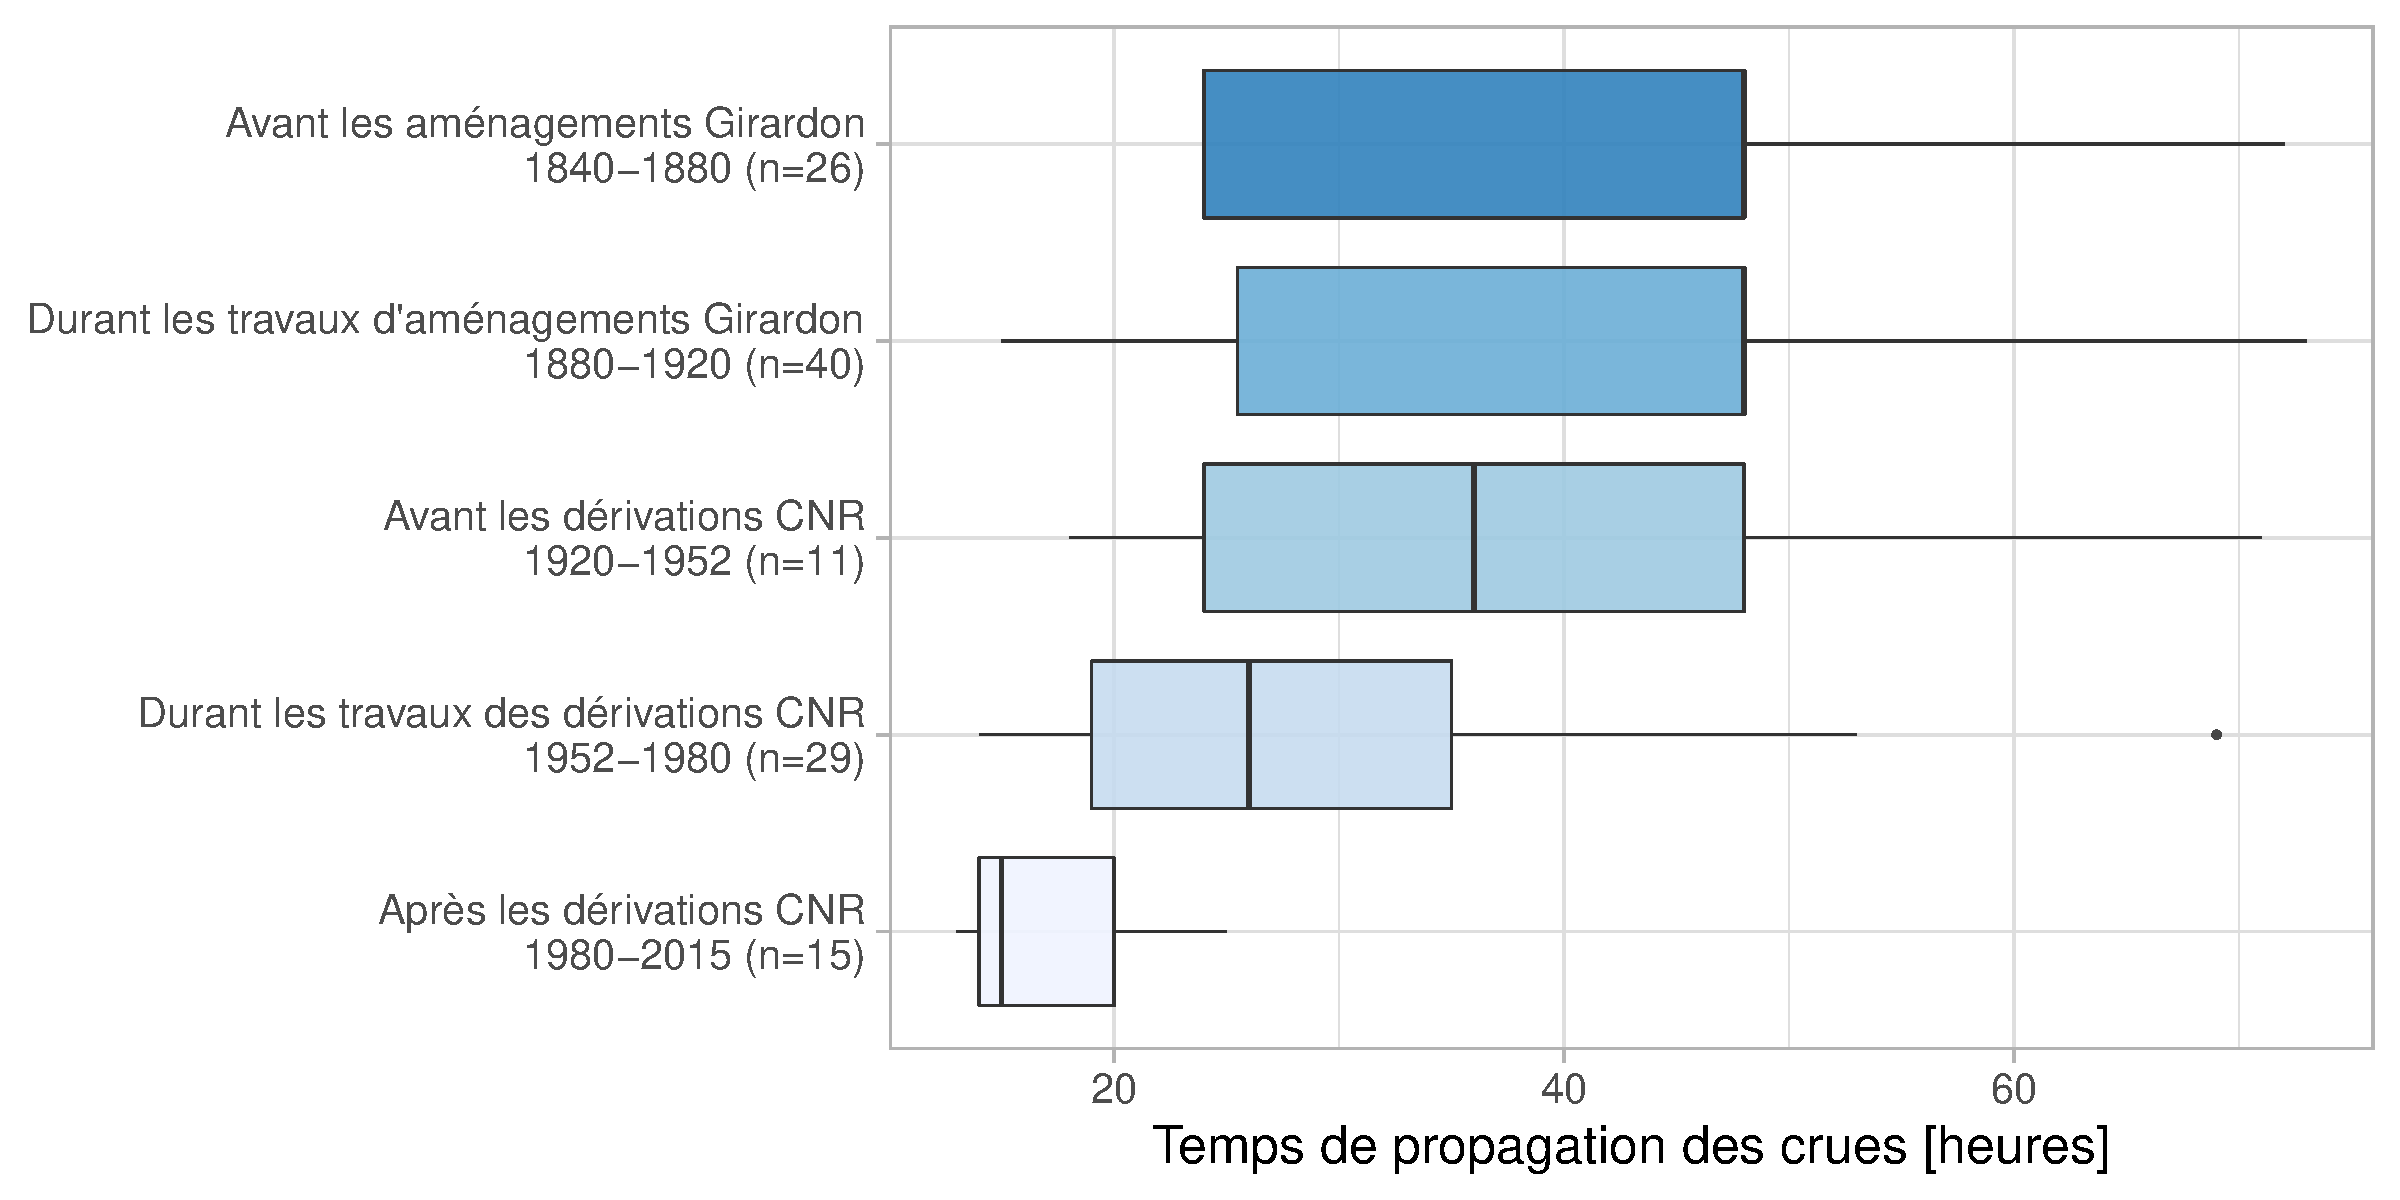
\includegraphics[width=.9\linewidth]{Chapitre2/Figures/BoxplotTprop_Fr.pdf}
	        \caption{Boites à moustache des temps de propagation de 121 crues océaniques entre l'aval de Lyon (stations de La Mulatière, Givors et Ternay) et Beaucaire (stations de Pont de Beaucaire et Beaucaire Restitution) pour 5 périodes d'aménagement du lit mineur (1840-2015).}
			\label{fig:BoxplotPropag}
		\end{figure}	

	\paragraph{} Les résultats sont présentés dans la figure \ref{fig:BoxplotPropag}. Le temps de propagation moyen pour parcourir les 250 km qui séparent l'aval de Lyon de Beaucaire est de 35 h pour l'ensemble de la période, on constate des variations de cette durée au cours des deux siècles d'aménagement du corridor fluvial. Le temps de transfert des crues fréquentes est en constante diminution depuis le début du XIX\textsuperscript{ème} siècle. En 175 ans, il est passé de 48 h (en valeur médiane) avant la construction des casiers Girardon, à 16 h après la construction des aménagements CNR. Les ouvrages Girardon semblent avoir, dès la fin du XIX\textsuperscript{ème} siècle, amorcé la réduction de ce temps de propagation des crues. La diminution importante des temps de propagation des deux dernières périodes d'étude indique que les aménagements hydroélectriques ont eu un impact encore plus important que les premiers aménagements en lit mineur. La précision des valeurs de temps de propagation est à relativiser, principalement pour les périodes anciennes au cours desquelles les relevés limnimétriques étaient effectués une ou trois fois par jour, causant un arrondi important. Le passage à trois données par jour en 1910, puis à des données horaires à partir de 1949, permet d'améliorer la précision de l'estimation des temps de propagation. On considère cependant que la médiane de l'ensemble des événements de chaque période est un indicateur pertinent, car une sous-estimation du temps de propagation de chacun des événement est tout aussi possible qu'une sur-estimation. 
	
	\paragraph{} Afin de vérifier les calculs de temps de propagation présentés ci-dessus, un modèle hydraulique a été utilisé pour modéliser la propagation d'une crue océanique entre Lyon et Beaucaire dans les conditions actuelles. Il s'agit du modèle MAGE OSR 1D qui modélise le cours du Rhône du lac Léman à la Méditerranée. Ce modèle sera présenté plus en détails en section \ref{sec:hydraul}. Une crue océanique type a été modélisée en se basant sur un débit de pointe de période de retour 10 ans pour le Rhône à Lyon, et 2 ans pour la Saône et l'Isère. Le débit des autres affluents est supposé égal au module de ces derniers. Les hydrogrammes en entrée ont été constitués à partir des hydrogrammes moyens de l'étude \citet{bard_actualisation_2018} pour le Rhône à Lyon, la Saône et l'Isère. Le décalage entre les pointes de crue des trois cours d'eau est basé sur les résultats de l'étude globale du Rhône \citep{rigaudiere_etude_2000} pour les événements de crue de type océanique. Dans ce scénario, la pointe de crue de l'Isère arrive en premier, suivie 24 h plus tard par la pointe du Rhône. La pointe de crue de la Saône arrive quant à elle 5 jours après la pointe de crue du Rhône en moyenne. Suite à la modélisation de ce scénario, on obtient un temps de propagation modélisé entre Ternay et Beaucaire de 18 h, ce qui est cohérent avec les 16 h estimées par l'analyse des limnigrammes. 

	\paragraph{} Les conséquences des aménagements en lit mineur sur la dynamique des crues vont probablement au delà des seuls temps de propagation, et peuvent être diverses. La forme moyenne des hydrogrammes peut avoir été modifiée et le pic de crue amplifié par une propagation devenue plus rapide. De plus, la concomitance du pic de crue du Rhône avec celui de ses affluents peut avoir été modifiée. Par exemple, les pics de crue de la Saône et de l'Isère sont systématiquement en retard sur celui du Rhône dans la plupart des scénarios de crue, y compris les crues de type océanique (\cite{parde_regime_1925}; \cite{rigaudiere_etude_2000}). Si le temps de propagation des crues du Rhône est réduit, alors l'écart de temps entre le pic de crue du Rhône et celui des affluents est augmenté, entrainant un débit moins important dans la partie aval du bassin versant. Ces conséquences pourraient être étudiées plus précisément en analysant les temps de propagation au niveau de stations limnimétriques intermédiaires dans la zone étudiée.

	\paragraph{} Le Rhône n'est pas le seul fleuve qui a subi ce type de transformations. Selon \citet{mitkova_analysis_2005}, des conséquences similaires ont été observées sur les crues du Danube. Entre 1899 et 2002, le temps de propagation entre Passau et Kienstock est passé de 40 h à seulement 15 h. C'est également le cas du Pô en Italie, qui a vu le temps de propagation de ses crues réduit suite à la construction d'aménagements en lit mineur \citep{di_baldassare_analysis_2009}. Toutefois, les limites de ces études proviennent de la disponibilité et de la fiabilité des données limnimétriques historiques datant d'avant les aménagements. C'est pourquoi l'étude des temps de propagation basée sur les limnigrammes anciens est peu répandue dans la littérature, contrairement aux études basée sur la modélisation hydraulique.
	
	\paragraph{} L'impact des aménagements sur la forme et le débit de pointe des crues n'a pas été quantifié ici. Il faudra garder à l'esprit lors de l'utilisation des données pour l'analyse fréquentielle que l'homogénéité des débits maximum annuels devra être vérifiée. Si des ruptures sont détectées dans les séries de débit, elles pourront notamment être attribuées à ces modifications anthropiques de la dynamique des crues. Cependant, l'impact de la diminution des temps de propagation sur le débit de pointe des crues peut être compensé par la moins bonne concomitance avec les affluents tel que décrit précédemment.

\FloatBarrier

\section{Données historiques : la base de données HISTRHÔNE (1300-2000)}
\label{sec:HISTRHONE}
	\subsection{Présentation de la base de données}

	\paragraph{} La base de données HISTRHÔNE (\url{histrhone.cerege.fr}) \citep{pichard_sept_2014} regroupe près de 1500 événements hydro-climatiques, depuis le XIII\textsuperscript{ème} siècle jusqu'à l'an 2000. Cet important travail d'archives qui s'est étalé sur plusieurs décennies, représente un apport majeur pour la connaissance de l'histoire hydrologique et climatique de la basse vallée du Rhône. La zone couverte par la base de données s'étale de la ville de Pont-Saint-Esprit jusqu'à la mer Méditerranée, en incluant les villes d'Avignon, Beaucaire et Arles, ainsi que l'ensemble de la Camargue (figure \ref{fig:MapHistrhone}). 
	
	\begin{figure}[h]
	\centering
		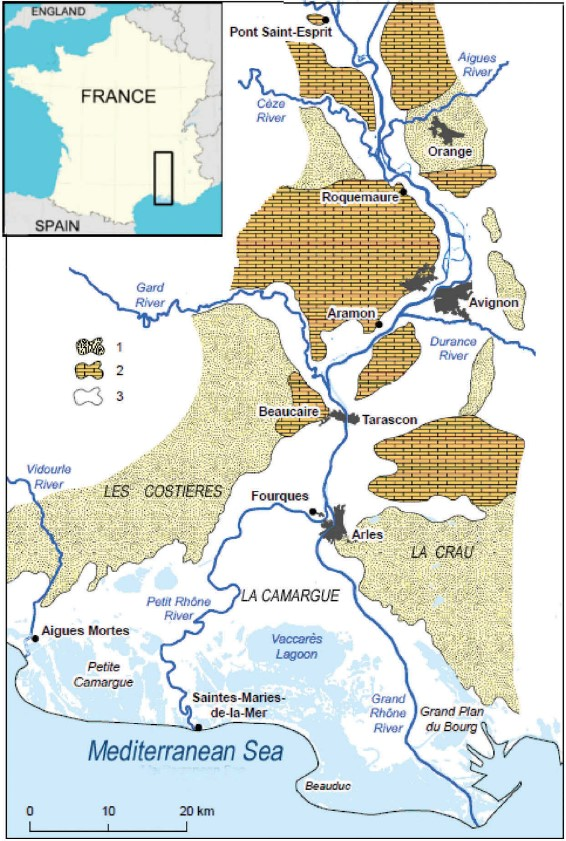
\includegraphics[width=.5\linewidth]{Chapitre2/Figures/HistrhoneMap.jpg}
        \caption{Localisation de la zone géographique couverte par la base HISTRHÔNE \citep{pichard_sept_2014} }
		\label{fig:MapHistrhone}
	\end{figure}
	
	\paragraph{} Les éléments historiques (témoignages, cartes...) qui correspondent à un même événement hydroclimatique sont regroupés et ces événements sont classés par type dans la base de données : crue, étiage, présence de glace ou gel du Rhône, inondation pluviale, submersion marine... Au-delà de la base de données, l'ouvrage «\textit{Sept siècles d'histoire hydroclimatique du Rhône d'Orange à la mer}» \citep{pichard_sept_2014} «\textit{offre une vue synoptique, à la fois des sources, de leur critique et des perspectives ouvertes par les premiers résultats que les auteurs ont pu en tirer comme contribution à une histoire hydroclimatique}». Il faut ajouter qu'une chronologie générale des événements est disponible, ainsi qu'une étude détaillée des échelles limnimétriques du bas Rhône qui «\textit{reprend l'ensemble des problèmes de mesures de hauteurs des crues dans l'histoire et tente de résoudre ces complications pratiques de métrologie}» \citep{pichard_hauteurs_2013} .
	
	\paragraph{} Dans la base de données HISTRHÔNE, les événements de crue sont classés en 6 catégories présentées dans le tableau \ref{tab:CatCrueHistrhone}. Ces catégories correspondent à différents niveaux de gravité, allant d'un Rhône "pleins bords" jusqu'à l'inondation extraordinaire. D'après \citet{pichard_sept_2014}, ces catégories permettent le classement des crues même en l'absence d'informations sur les hauteurs ou les débits : «\textit{Un seuil de hauteur unique présente l'intérêt de la simplicité et de l'universalité. On peut ainsi choisir la limite évidente du débordement hors du lit mineur, surtout si cette limite est bien connue et sans ambiguïté, mais il faut alors renoncer à pondérer des types de crues que les sources anciennes ne permettent pas de discriminer. [...] il faut se résoudre à choisir le type de crue en fonction de critères indirects, mais tout aussi pertinents que les hauteurs et les débits. On s'appuie sur la comparaison avec la période des hauteurs mesurées en continuité, mais aussi sur les conséquences et les dommages, sur l'extension de la crue dans la plaine proximale ou distale, sur sa généralisation dans une partie ou la totalité du territoire étudié}». Si la détermination d'un seuil de hauteur ou de débit n'est pas essentielle pour l'analyse de l'historique hydroclimatique, elle l'est en revanche pour l'utilisation de ces données dans le cadre de l'analyse fréquentielle des crues.  Il faudra donc veiller à la correspondance entre ces catégories basées sur des informations très diverses.
	
\begin{table}[h]
	\centering
	\caption{Classification des événements de crue de la base HISTRHÔNE. Les estimations de débit proviennent de \citet{pichard_hydro-climatology_2017}. Les ségonnaux représentent des parcelles potentiellement exploitables comprises entre un fleuve et ses digues.}
	\label{tab:CatCrueHistrhone}
%	\resizebox{\columnwidth}{!}{
		\begin{tabular}{|m{0.8cm}|m{3.6cm}|m{7.6cm}|m{3cm}|}
		\hline
		Code &
		  Libellé &
		  Description &
		  Débit estimé [m\textsuperscript{3}/s] \\ \hline
		Ci &
		  Crue de gravité indéterminée &
		  Crue sans aucune précision : pas d'indice de débordement ni de gravité (incertitude totale) &
		  X \\ \hline
		Cd &
		  Crue avec indice de débordement &
		  Débordement avéré mais sans précision relative à son étendue ou sa gravité (incertitude partielle) &
		  X \\ \hline
		C1 &
		  Hautes eaux &
		  
\textbf{Rhône "pleins bords", "gros Rhône" sans débordement}. Le Rhône reste dans son lit mineur mais implique une surveillance constante aux digues &
		  X \\ \hline
		C2 &
		  Crue avec débordement sans gravité et/ou localisé &
		 
\textbf{Débordement limité}, sans gravité majeure ou bien localisée (ségonnaux, prés/chemins inondés, eaux sur les quais, dégâts mineurs sur digues) &
		 5200 \\ \hline
		C3 &
		  Crue et inondation de gravité intermédiaire &
		  
\textbf{Inondation notable} avec dégâts avérés au caractère destructeur et/ou extension de crue &
		  7200 \\ \hline
		C4 &
		  Crue et inondation extrêmes &
\textbf{Inondation extraordinaire} avec dégâts exceptionnels (pertes humaines et animales, intérieurs des villes inondés, dégradations de digues en grand nombre) et extension de crue &
		  9000 \\ \hline
		\end{tabular}
%	}
\end{table}
	
\FloatBarrier

	\subsection{Ordre de grandeur du débit de pointe des crues de la base HISTRHÔNE}
	
	\paragraph{} L'exploitation des crues historiques pour l'analyse fréquentielle nécessite d'estimer un ordre de grandeur du débit de pointe de ces événements. Plus précisément, il est possible d'exploiter statistiquement les données historiques à condition d'en déterminer un seuil de perception. Il s'agit ici de garantir que toutes les crues dont le débit fut supérieur à un seuil de perception ont laissé une trace dans les archives. Dans le cas des événements de la base HISTRHÔNE, il est possible de faire correspondre un seuil de perception à chacune des catégories. L'analyse fréquentielle des crues qui découle de ces seuils de perception sera réalisée au chapitre \ref{chap:ch4}, mais il faut tout d'abord en faire une première estimation. \citet{pichard_hydro-climatology_2017} en donnent un premier ordre de grandeur (tableau \ref{tab:CatCrueHistrhone}) en calculant la moyenne du débit à Beaucaire des crues de chaque catégorie pour les événements du XX\textsuperscript{ème} siècle, en utilisant les données de la banque Hydro (\url{www.hydro.eaufrance.fr}). Néanmoins, l'utilisation d'une moyenne ne reflète pas exactement le concept de seuil de perception présenté plus tôt, mais cela permet d'en connaitre l'ordre de grandeur. Le débit de la plus petite crue de chacune des catégories serait plus adapté. 
	
	\begin{figure}[h]
	\centering
		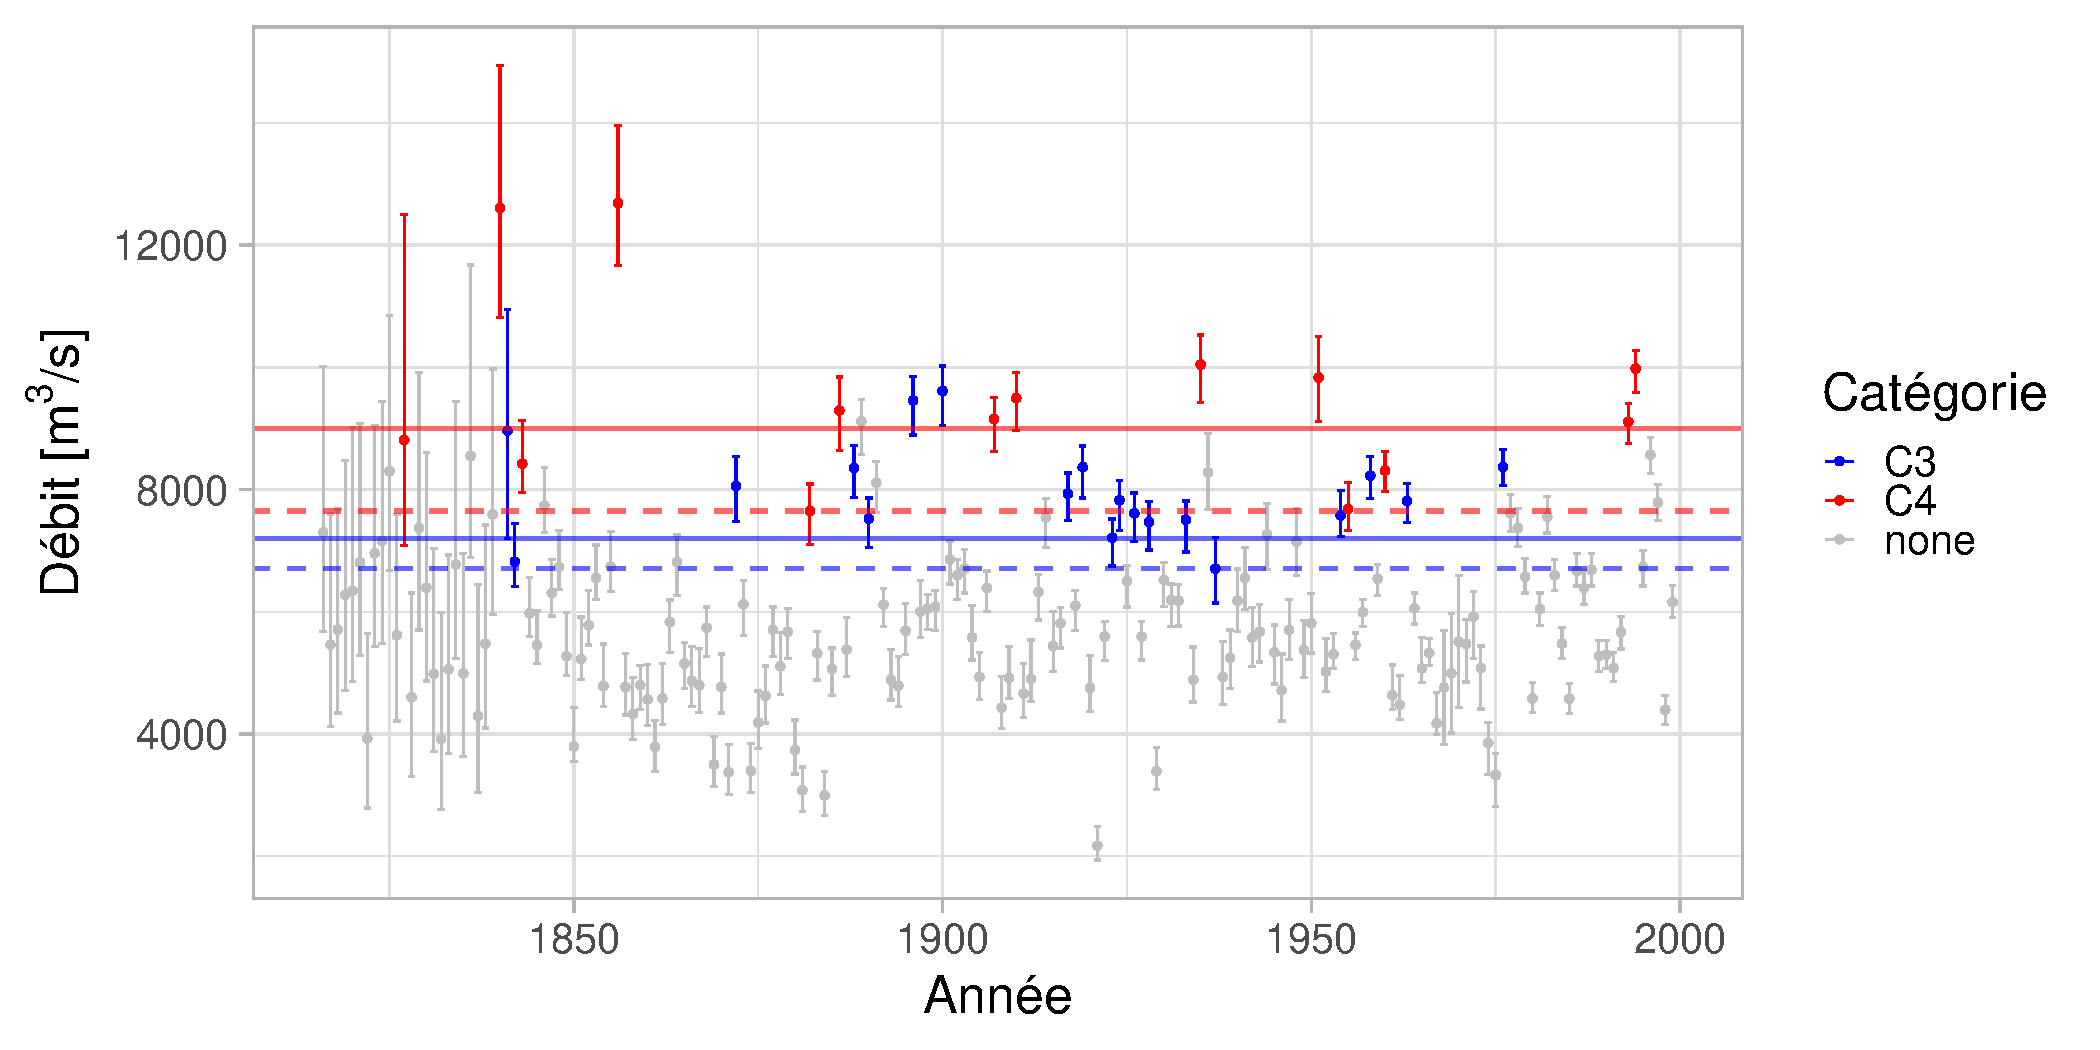
\includegraphics[width=.9\linewidth]{Chapitre2/Figures/C3-C4_SystematicPeriod-FR.pdf}
        \caption{Débit maximum annuel à Beaucaire de 1816 à 2000 (estimations tirées du chapitre \ref{chap:ch3}). Les barres d'erreur représentent l'incertitude à 95\%, les droites horizontales représentent l'estimation de \citet{pichard_hydro-climatology_2017} (trait plein) et le débit estimé de la plus petite crue de chacune des catégories (trait pointillé).}
		\label{fig:C3-C4_Syst}
	\end{figure}
		
	
	\paragraph{} Les débits maximum annuels avec incertitude de 1816 à 2020 (dont le calcul sera détaillé au chapitre \ref{chap:ch3}) sont croisés avec les catégories C3 et C4 de la base HISTRHÔNE. La période commune de ces deux jeux de données s'étend de 1816 à 2000. Seules ces deux catégories sont retenues car elles contiennent des crues responsables de dégâts notables et sont susceptibles d'être informatives pour l'analyse fréquentielle menée au chapitre \ref{chap:ch4}. On remarque sur la figure \ref{fig:C3-C4_Syst} que les limites entre catégories sont "perméables", du moins pour cette période "témoin" de 1816 à 2000 : des crues appartenant à la catégorie C3 sont plus fortes que certaines crues de la catégorie C4. Par exemple, le débit maximum de l'année 1900, classée C3, atteint 9614 m\textsuperscript{3}/s, alors que les 8310 m\textsuperscript{3}/s de l'année 1960 sont classés en catégorie C4. A ce propos, \citet{pichard_sept_2014} expliquent que : «\textit{Ce sont les catégories C3 et C4 qui offrent les plus grandes difficultés de discrimination. Pour la catégorie C3, la distinction avec les crues localisées est parfois délicate [...] Il y a une gradation certaine au sein de cette catégorie [...] Ce sont ainsi les crues dites extrêmes qui permettent de délimiter les passages dans la catégorie supérieure, beaucoup plus nette. Les crues extrêmes (C4) entrainent des destructions importantes, s'introduissent au cœur des villes et dans les maisons, couvrent des territoires les plus étendus et transforment la Camargue et le Plan du Bourg d'Arles en mers à perte de vue.}» De plus, certaines crues ne sont pas classées bien que supérieures à certaines crues C4. Par exemple, le débit maximum annuel de l'année 1889 atteint 9115 m\textsuperscript{3}/s mais n'est classé dans aucune des deux catégories, alors que la plus petite des crues de la catégorie C4 n'atteint que 7649 m\textsuperscript{3}/s (1882). 
	
	\paragraph{} La moyenne des crues de chaque catégorie sur la période 1816-2000 est plus forte que celle présentée par \citet{pichard_hydro-climatology_2017} car cette dernière est calculée uniquement sur les données XX\textsuperscript{ème} siècle (tableau \ref{tab:Qcateg}). Ces valeurs moyennes permettent d'avoir un ordre de grandeur du débit de ces catégories mais ne répondent pas à la définition du seuil de perception. Le débit de la plus petite crue de chaque catégorie représente une estimation plus adéquate, même si les limites entre catégories ne semblent pas univoques en termes de débit. Ces constatations encouragent la considération d'une incertitude autour du seuil de perception. De plus, le fait que certains débits maximum annuels supérieurs à la plus petite des crues C4 (1816-2000) ne correspondent à aucune des deux catégories encourage à la méfiance quand à l'exhaustivité des données sur l'ensemble de la période. Ces questions d'incertitudes autour du seuil de perception et de l'exhaustivité des données historiques seront abordées plus en détails dans le chapitre \ref{chap:ch4}.

	\begin{table}[h]
	\centering
	\caption{Débits caractéristiques des catégories de la base HISTRHÔNE. Les estimations de \citet{pichard_hydro-climatology_2017} représentent la moyenne des débits maximum annuels du XX\textsuperscript{ème} siècle. Les autres colonnes correspondent à la moyenne des débits maximum annuels de chaque catégorie et le débit de la crue la plus petite de chacune des catégories basés sur la chronique continue estimée de 1816 à 2000 au chapitre \ref{chap:ch3}.} 
	\label{tab:Qcateg}
		\begin{tabular}{|c|c|c|c|}
		\hline
		Catégorie HISTRHÔNE & \citet{pichard_hydro-climatology_2017} & Moyenne 1816-2000 & Minimum 1816-2000\\ \hline
		C3  & 7200 m\textsuperscript{3}/s  & 7970 m\textsuperscript{3}/s    & 6706 m\textsuperscript{3}/s   \\ \hline
		C4  & 9000 m\textsuperscript{3}/s  & 9506 m\textsuperscript{3}/s    & 7649 m\textsuperscript{3}/s   \\ \hline
		\end{tabular}
	\end{table}
	
	\subsection{Évolution temporelle de la vulnérabilité aux inondations}
	\label{subsec:EvolVuln}
	
	\paragraph{} Le classement des crues dans la base HISTRHÔNE est basé sur des critères indirects, différents du débit et de la hauteur d'eau, tels que : «\textit{les conséquences et les dommages, [...] l'extension de la crue dans la plaine proximale ou distale, [...] sa généralisation dans une partie ou la totalité du territoire étudié}» \citep{pichard_sept_2014}. Les mêmes critères sont utilisés pour catégoriser les crues du XIV\textsuperscript{ème} siècle et celles du XX\textsuperscript{ème} siècle. 
	
	\begin{figure}[h]
	\centering
		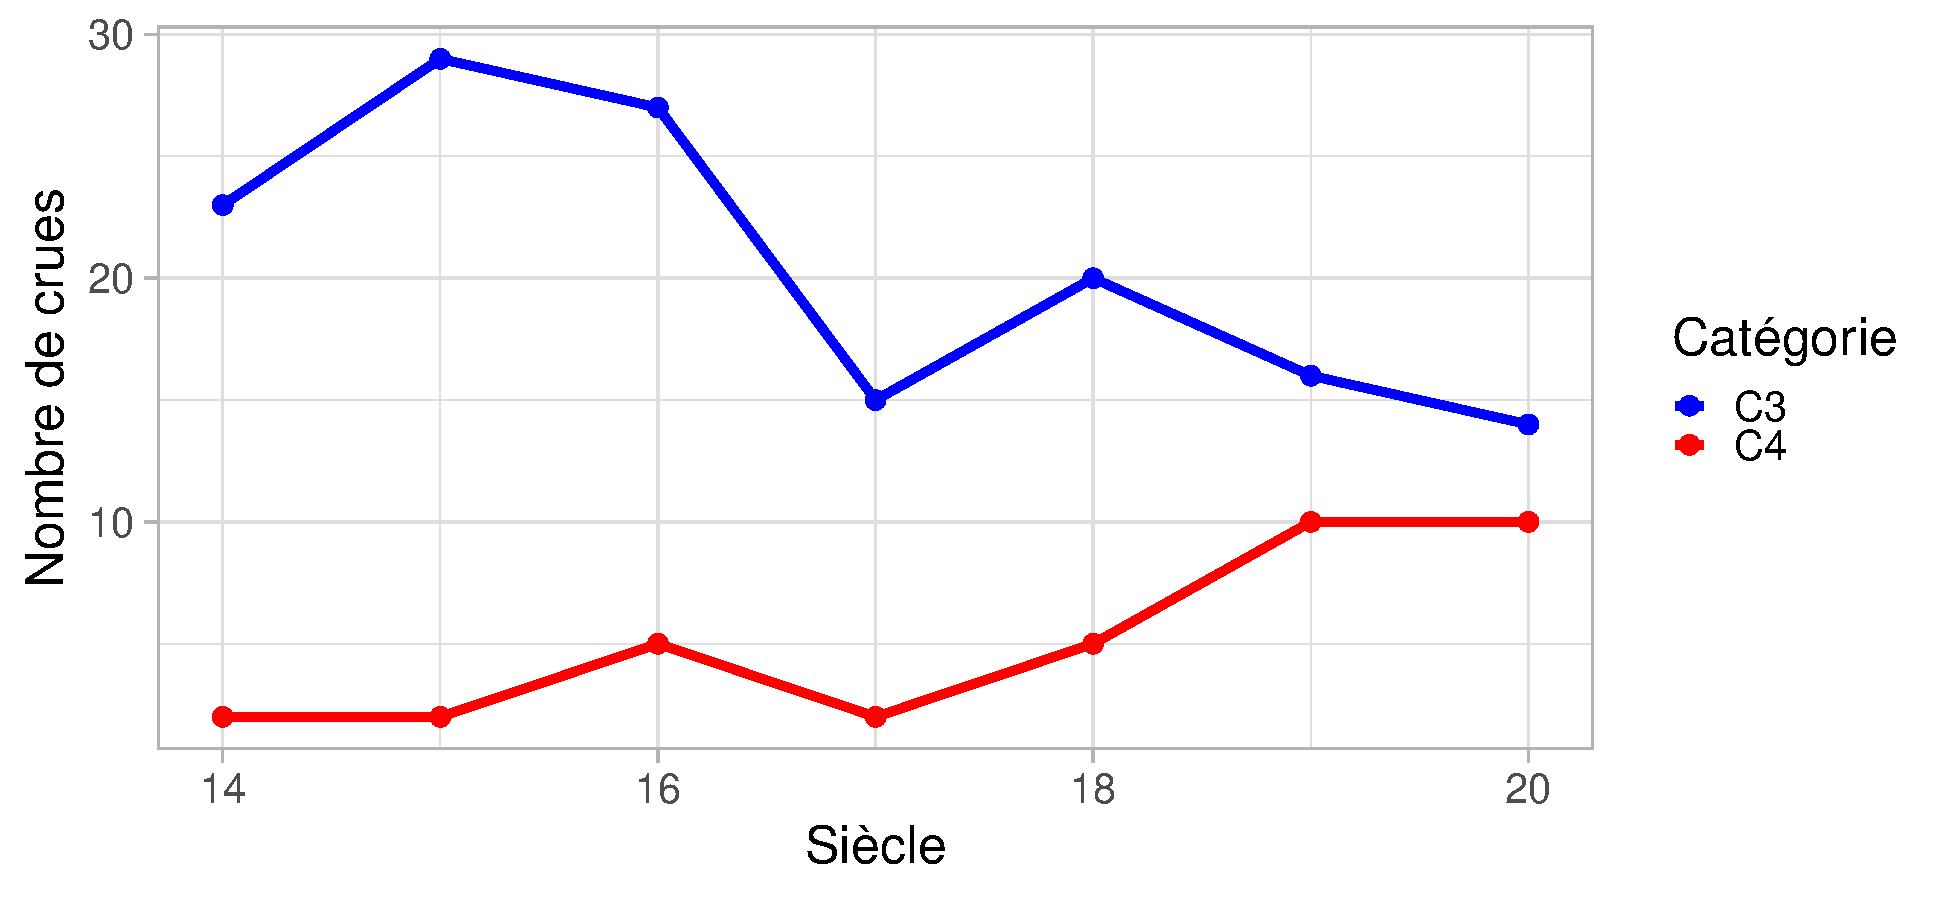
\includegraphics[width=.8\linewidth]{Chapitre2/Figures/Nb_C3-C4.pdf}
        \caption{Nombre de crues par siècle dans les catégories C3 et C4 de la base HISTRHÔNE, du XIV\textsuperscript{ème} au XX\textsuperscript{ème} siècle.}
		\label{fig:Nb_C3C4}
	\end{figure}	
	
	\paragraph{} La figure \ref{fig:Nb_C3C4} témoigne de l'évolution de la perception des crues des catégories C3 et C4. On constate une diminution du nombre de crues C3 à partir du XVII\textsuperscript{ème} siècle, au profit des crues de la catégorie C4. Plusieurs facteurs peuvent expliquer cette évolution. \citet{pichard_sept_2014} l'attribuent notamment aux actions anthropiques : «\textit{La reconstruction et l'extension des digues, le défrichement des rives, l'essor urbain, tout concourt à concentrer les écoulements lors des plus grands épisodes tout en atténuant ou même en faisant disparaître les débordements ordinaires ou moyens (C2 et C3)}». 
	
	\paragraph{} La vulnérabilité des populations ripariennes évolue au cours du temps, et ce partout dans le monde \citep{kron_flood_2002}. De nombreux exemples de cette évolution existent, y compris en France, comme démontré par \citet{boudou_assessing_2016} pour les bassins versants du Doubs et du Tarn. La basse vallée du Rhône ne fait pas exception à la règle \citep{piegay_observatoire_2022}. De plus, la perception des dommages par les populations est elle aussi variable et est la conséquence de nombreux facteurs, pouvant être d'origine physique (niveau de protection aux inondations, rupture de digues, densité de population...) ou médiatique (contexte sociétal, politique, religieux...). Ainsi, on observe au sein des données de crue de la base HISTRHÔNE des fluctuations dont l'origine n'est probablement pas seulement hydroclimatique. 
	
\FloatBarrier

\section{Estimation du débit des événements historiques}
\label{sec:hydraul}
	\paragraph{} Dans l'optique de l'utilisation des données de crues historiques de la base HISTRHÔNE pour l'analyse fréquentielle, la connaissance du débit de chacun des événements peut s'avérer utile. Cependant, l'estimation de ces débits dans un contexte historique est bien plus complexe que dans le cas de stations hydrométriques et peut être impacté par de fortes incertitudes. Tout d'abord, la mesure limnimétrique n'est pas continue et repose sur des témoignages sporadiques, donnant des informations très dispersées spatialement. Il peut également être complexe de reconstituer la hauteur d'eau correspondant à la pointe de la crue et il est encore plus complexe de reconstituer la dynamique temporelle de la crue. Ensuite, l'estimation d'un débit basée sur la hauteur observée n'est pas évidente en l'absence de jaugeages. Le schéma hydrométrique classique ne peut donc être suivi. Une des solutions est l'utilisation d'un modèle hydraulique. Cependant, l'élaboration d'un tel modèle est notamment conditionnée à l'existence ou à la reconstitution de données topographiques et bathymétriques contemporaines à la crue étudiée. La modélisation hydraulique unidimensionnelle (1D) est très simplifiée car elle fait l'hypothèse que les quantités (hauteur d'eau, vitesses et direction de l'écoulement) sont uniformes au sein d'une section en travers. Ce type de modèle n'est pas aussi précis qu'un modèle 2D, mais il demande en revanche une description bien moins fine de la géométrie de la rivière, ce qui est avantageux dans le cas de reconstitutions historiques pour lesquelles ces données sont rares. Le but de l'utilisation de la modélisation hydraulique dans ce chapitre est l'inverse du but habituel. En effet, on cherche ici à identifier le débit ayant engendré les niveaux d'eau relevés lors des crues, et non à estimer les niveaux atteints pour un débit donné. Pour cela, il est possible pour un événement donné d'encadrer le débit de la crue dans un intervalle, en approchant la hauteur d'eau atteinte en un point donné qui est extraite de la base HISTRHÔNE avec la hauteur modélisée en ce même point. Dans la section qui suit, la piste de l'estimation du débit des crues historiques par la modélisation hydraulique 1D est explorée afin d'évaluer si les limites de cet exercice sont surmontables pour des événements antérieurs à l'installation de l'échelle limnimétrique de Beaucaire. Ces estimations de débit pourraient ensuite être utilisées dans le cadre l'analyse fréquentielle des crues. Des hypothèses simplificatrices du modèle hydraulique seront notamment explorées afin de limiter la quantité d'informations nécessaires.

	\FloatBarrier
	 \subsection{Adaptation du modèle MAGE OSR 1D à l'étude des crues historiques à Beaucaire}
	 
	 \paragraph{} L'Observatoire des Sédiments du Rhône (OSR) (\url{www.graie.org/osr}) étudie les flux sédimentaires ainsi que les pollutions associées à ces sédiments sur les 545 km du cours du Rhône du lac Léman à la Méditerranée. A ce titre, un modèle hydraulique a été développé sur l'ensemble du linéaire (\cite{dugue_accounting_2015}; \cite{launay_numerical_2019}). Ce modèle se base sur le code de calcul MAGE \citep{souhar_approach_2009} qui résout les équations de Barré-de-Saint-Venant 1D ainsi que la formule de perte de charge de Manning-Strickler. Le modèle inclut également les tronçons les plus à l'aval des principaux affluents, ainsi qu'une représentation du fonctionnement des aménagements hydroélectriques. Il a été calé et validé jusqu'au débit des crues non-débordantes (soit un débit de période de retour d'environ 10 ans pour la partie à l'aval de Lyon). La géométrie du lit est définie par des profils en travers réalisés environ tous les 500 m. Le modèle n'étant pas prévu pour représenter les crues débordantes, les profils en travers s'étendent jusqu'aux limites du lit moyen, aussi appelé lit majeur actif (c'est-à-dire la partie mouillée par les crues fréquentes). Les débordements, ruptures de digues et surverses ne sont donc pas pris en compte (sauf quelques exceptions locales) et la géométrie au-delà des digues est représentée par des murs verticaux artificiels dont les frottements sont négligés. 
	 
	 \paragraph{} Le modèle MAGE OSR 1D est adapté à l'étude de la dynamique hydro-sédimentaire à long terme, mais ne peut en l'état être utilisé pour la modélisation des crues à Beaucaire : plusieurs adaptations et hypothèses simplificatrices sont nécessaires. Tout d'abord, il est inutile de conserver la totalité des biefs, le modèle s'étendant du lac Léman à la Méditerranée. Afin de limiter la quantité de données anciennes nécessaire, ainsi que le temps de calcul, la limite amont du modèle est définie à l'aval immédiat de la confluence avec la Durance, environ 15 km à l'amont de Beaucaire. La limite amont aurait pu être fixée à la confluence avec le Gardon (dernier affluent du Rhône, 5 km à l'amont de Beaucaire). Cependant, il est complexe de reconstituer la bathymétrie historique de cette confluence notamment à cause des importants changements morphologiques suite à l'installation des aménagements CNR (figure \ref{fig:LimAmont}). Dans un but de simplification, le Gardon sera représentée par un apport latéral direct dans le modèle, ce qui ne nécessite pas la reconstitution de sa bathymétrie. 
	 
	 \begin{figure}[h!]
		\centering
	    \includegraphics[width=\linewidth]{Chapitre2/Figures/LimAmont.pdf}
        \caption{Confluence du Gardon et du Rhône environ 5 km à l'amont de Beaucaire pour la période pré-aménagements CNR à gauche (carte IGN 1950) et la période actuelle à droite (carte IGN actuelle). Source : \url{www.geoportail.gouv.fr}.}
		\label{fig:LimAmont}
	\end{figure}
	 
\FloatBarrier	 
	 
	\paragraph{} La limite aval originelle du modèle est représentée par la mer Méditerranée pour les deux biefs du delta, le Petit et le Grand-Rhône. Étant donné les fortes évolutions bathymétriques de l'embouchure du Grand-Rhône représentées sur la figure \ref{fig:Embouch} \citep{pichard_les_2014}, il serait utile de pouvoir fixer la limite aval plus à l'amont. Il existe un nombre important de hauteurs d'eau pour les crues historiques à l'échelle reconstituée des marches du port d'Arles \citep{pichard_les_1995}, la limite aval pourrait donc fixée au niveau de cette échelle, au PK 282.2, à condition que l'impact sur les hauteurs modélisées à Beaucaire soit négligeable.
	
	\begin{figure}[h]
		\centering
	    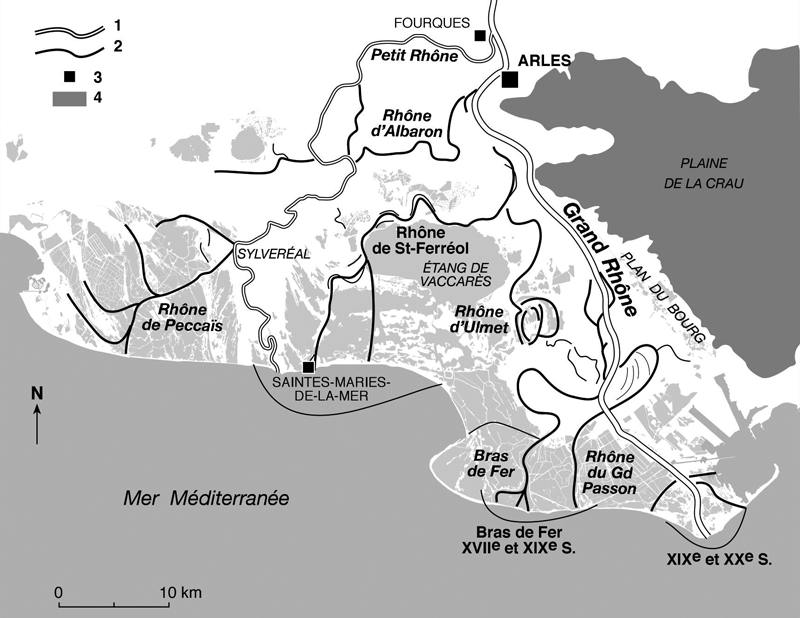
\includegraphics[width=.6\linewidth]{Chapitre2/Figures/EvolEmbouch.jpg}
        \caption{Évolutions morphologiques du delta du Rhône du XIV\textsuperscript{ème} à aujourd'hui \citep{pichard_les_2014}). Beaucaire se situe environ 15 km à l'amont de Fourques. 1 : bras actifs de nos jours, 2 : tracés des bras hérités, 3 : Principales localités, 4 : plaine de la Crau.}
		\label{fig:Embouch}
	\end{figure}

	\paragraph{} L'influence du déplacement de la limite aval du modèle peut être étudiée. Une simulation est réalisée pour un débit constant (et non-débordant) de 4000~m\textsuperscript{3}/s en limite amont pour les deux scénarios. La figure \ref{fig:DifMerArles} présente la différence de cote (hauteur d'eau) entre les scénarios "limite aval au niveau de la mer" et "limite aval au niveau d'Arles", pour le bief reliant Beaucaire à la diffluence du Petit Rhône. On remarque que la différence est maximale au niveau de la diffluence (7~cm). A Beaucaire, la différence de hauteur est inférieure à 3~cm. On supposera donc que le choix de la limite aval au niveau du Grand-Rhône n'a que peu d'impact sur la cote à Beaucaire et que l'on pourra se passer de reconstituer les formes anciennes de la partie aval de ce bief. 
	 
	\begin{figure}[h]
	\centering
		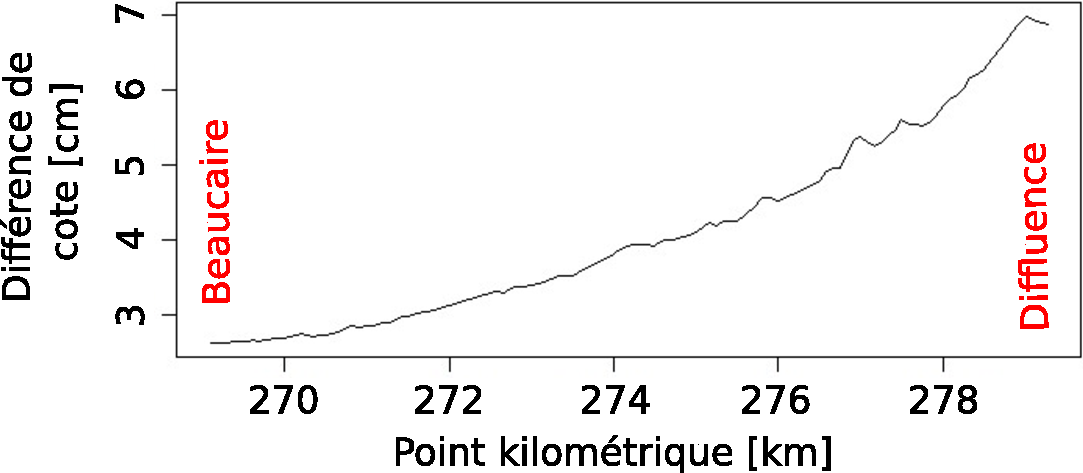
\includegraphics[width=.7\linewidth]{Chapitre2/Figures/DiffMerArles.pdf}
        \caption{Différence de hauteur d'eau sur le bief Beaucaire-Diffluence pour un débit permanent de 4000~m\textsuperscript{3}/s et pour une limite aval au niveau de la mer ou au niveau de la ville d'Arles. La ville d'Arles se situe environ 2 km à l'aval de la diffluence (à droite).}
		\label{fig:DifMerArles}
	\end{figure}			 
	 	
\FloatBarrier

	\paragraph{} Afin d'adapter la géométrie des sections à des débits importants, des points supplémentaires ont été ajoutés au modèle pour représenter le lit majeur. L'altitude de ces points est basée sur les données MNT de la base de données topographique (BDT) du Rhône dont les mesures ont été réalisées en 2010 dans le cadre du Plan Rhône. Les sections en travers sont prolongées jusqu'aux digues de protection actuelles (figure \ref{fig:Elarg}) qui protègent des débordements au moins jusqu'au niveau de la crue de 2003, soit une crue environ centennale. Étant donné que la simulation sera en régime permanent, aucun casier de débordement ne sera implémenté dans le modèle, ces derniers ayant uniquement un intérêt dans le cas de simulations en régime transitoire pour la prise en compte du laminage des crues. De plus, il peut être particulièrement complexe d'estimer le volume de casiers de débordement dans le cas de crues très anciennes.
	
	\begin{figure}[h]
	\centering
		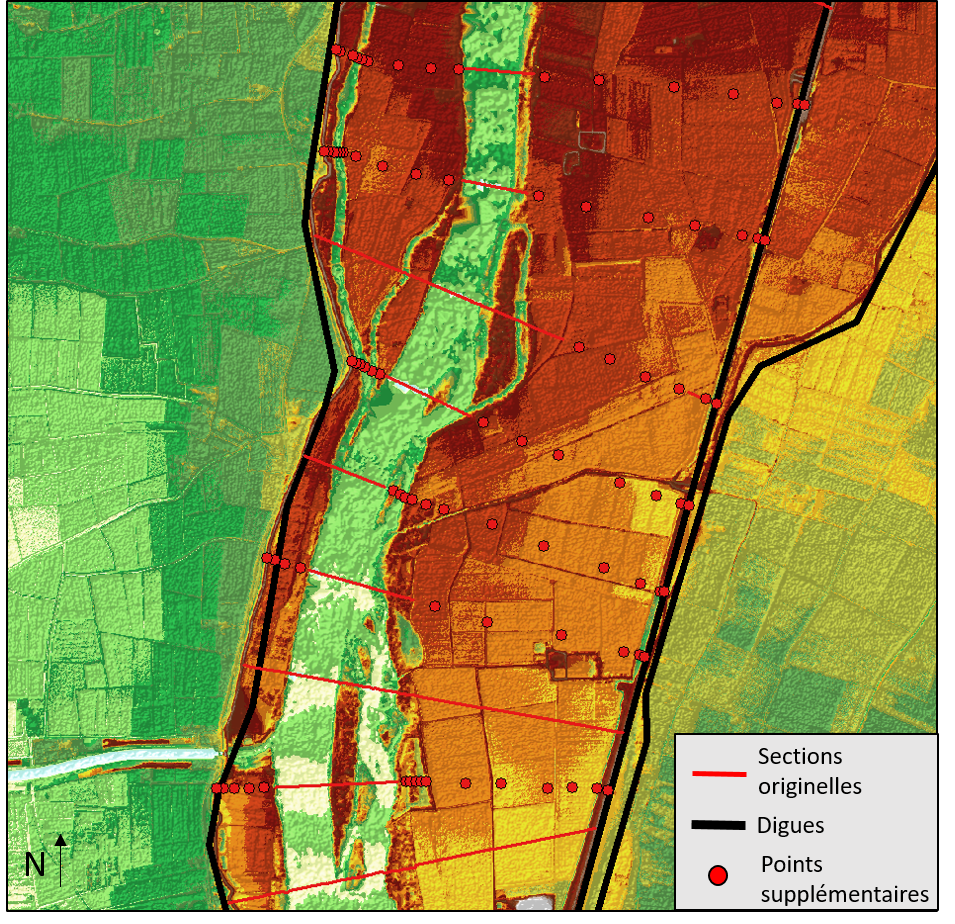
\includegraphics[width=.6\linewidth]{Chapitre2/Figures/Elarg.png}
        \caption{Élargissement des sections en travers du modèle jusqu'aux limites du lit majeur (digues). On se trouve ici entre Beaucaire et Arles, 4 km à l'amont de la diffluence. L'altitude des points est basée sur le MNT de la BDT Rhône de 2010 qui est affiché en arrière plan. Les couleurs vertes correspondent à de faibles altitudes, les couleurs sombres à des altitudes plus importantes.}
		\label{fig:Elarg}
	\end{figure}		
	
	\paragraph{} Afin de se placer dans le contexte historique pré-aménagements CNR, les aménagements présents dans le modèle sont supprimés. Il s'agit de l'usine de Beaucaire, du barrage de Vallabrègues, ainsi que du seuil de Beaucaire. La topologie du modèle suite aux simplifications présentées dans cette section est représentée dans la figure \ref{fig:Mageavap} (droite).
	
	\begin{figure}[h]
	\centering
		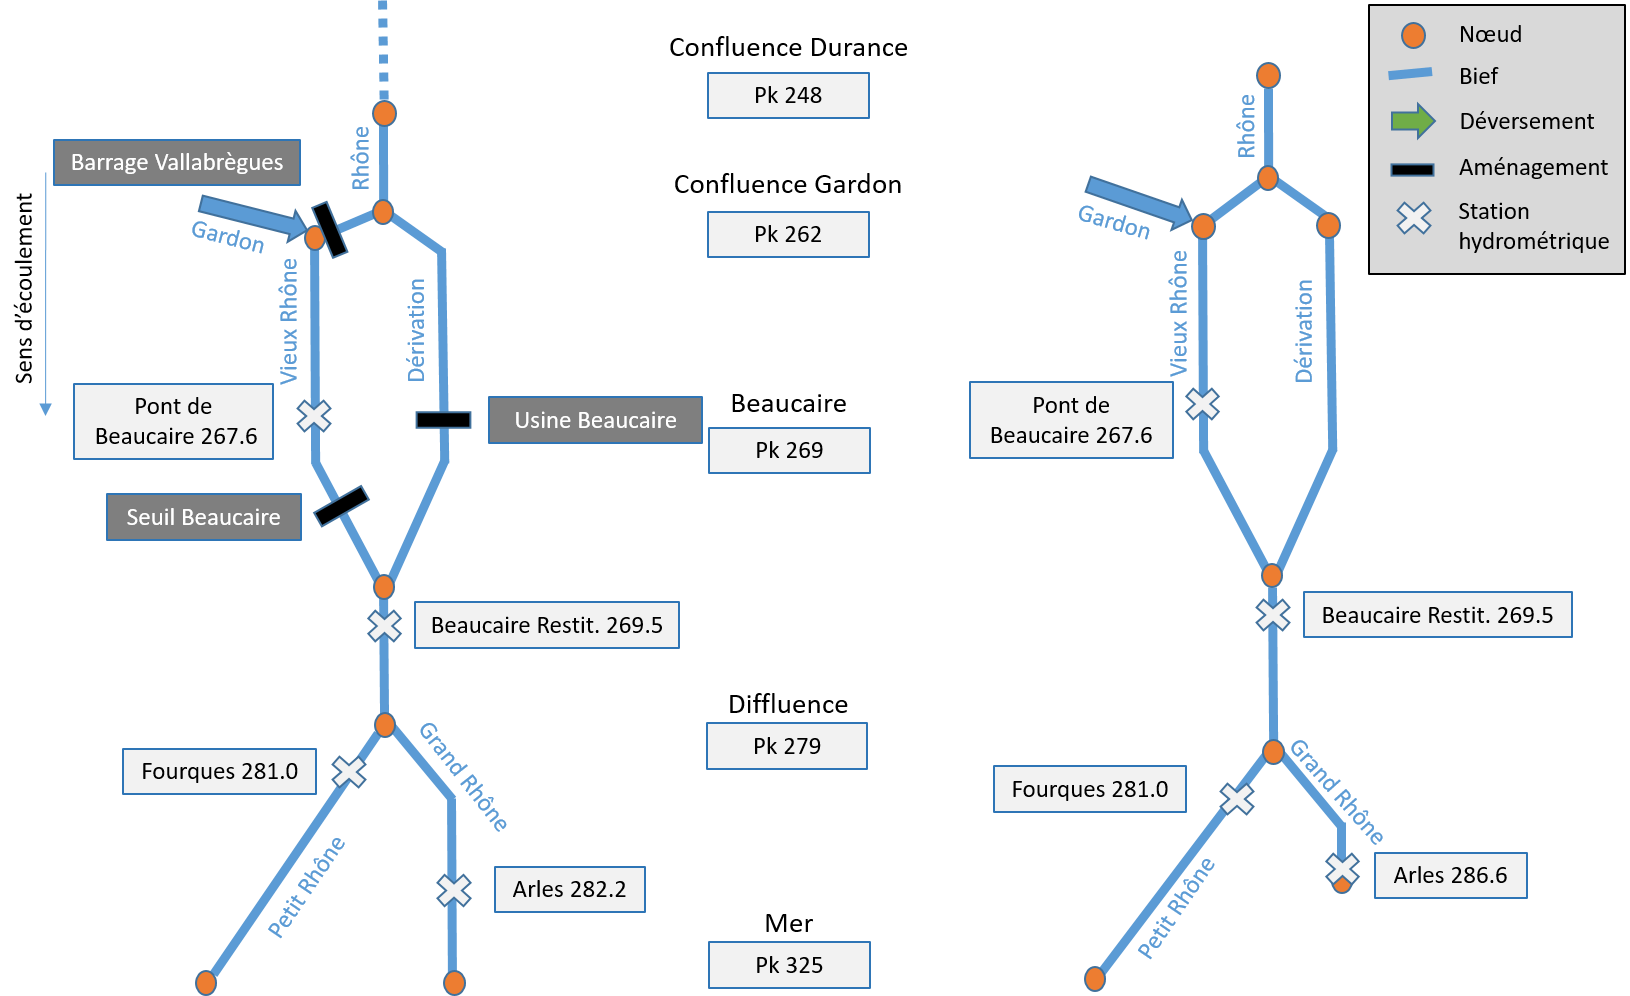
\includegraphics[width=\linewidth]{Chapitre2/Figures/MAGERh_AvAp.png}
        \caption{Topologie du modèle avant (gauche) et après simplifications (droite) : suppression des aménagements récents et limite aval du bief du Grand-Rhône ramenée à Arles.}
		\label{fig:Mageavap}
	\end{figure}		
	
\FloatBarrier	
	\subsection{Simplification du modèle Rhône OSR 1D}
		
	\paragraph{} La sensibilité du modèle hydraulique à plusieurs scénarios a été testée afin de connaitre l'impact de la prise en compte (ou de la non-prise en compte) précise de ces scénarios dans le cadre de reconstitutions historiques. La référence de ces tests est le modèle présenté à la section précédente, pour lequel les aménagements hydroélectriques ont été supprimés, les sections en travers ont été élargies jusqu'aux limites du lit majeur, et la limite aval du Grand Rhône a été fixée à Arles. Les simulations suivantes représentant diverses hypothèses seront donc comparées à cette simulation de référence. La différence de hauteur au niveau de la station de Pont de Beaucaire sera notamment étudiée.
	
	\paragraph{} On cherche à reproduire ici une crue centennale similaire à la crue de décembre 2003 au cours de laquelle le débit à Beaucaire était d'environ 11~500~ m\textsuperscript{3}/s \citep{medd_debit_2005}. La condition limite amont (nœud à l'aval de la confluence avec la Durance) est représentée par un hydrogramme permanent de 10~000~ m\textsuperscript{3}/s. La confluence du Gardon est représentée par un apport latéral constant de 1500~m\textsuperscript{3}/s, ce qui correspond environ à une crue décennale à la station du Rémoulins, la station située la plus à l'aval sur le Gardon (\url{hydro.eaufrance.fr}). Le débit du Gardon pendant la crue de décembre 2003 a atteint environ 1250 m\textsuperscript{3}/s à Rémoulins, mais cette valeur est fortement incertaine. La limite aval pour le bief du Petit Rhône est représentée par un niveau de la mer Méditerranée de 0.136~m~NGF~IGN69. La limite aval du Grand Rhône est représentée par un limnigramme constant à 7.03~m~NGF~IGN69, soit la hauteur maximale enregistrée lors de la crue de 2003. Le calage des coefficients de frottement (Strickler) du modèle OSR \citep{launay_zabr-osr_2017} est conservé, bien que ces derniers ne soient validés que jusqu'à la crue décennale. Le pas de temps de simulation est de 60 secondes, et l'événement est simulé pendant une durée de 10 heures afin d'aboutir à une convergence satisfaisante.

\FloatBarrier	

	\subsubsection{Sensibilité à la présence d'aménagements hydroélectriques}
	
		\paragraph{} Les aménagements hydroélectriques CNR ont été construits entre 1967 et 1970 et ont une influence sur la ligne d'eau à Beaucaire. Ces aménagements sont représentés dans le modèle OSR originel \citep{launay_zabr-osr_2017} sous forme de lois d'ouvrage qui seront reprises ici. Par exemple, le barrage de Vallabrègues est représenté par une loi de type seuil/déversoir avec une cote de déversement de 16.63~m, une largeur déversante de 176~m, et un coefficient de débit de 0.4. La vanne de fond est représentée par un orifice rectangulaire dont la cote de déversement correspond à un niveau de 2.03 m, la cote de mise en charge à un niveau de 6.1~m, et la cote de mise en charge maximale à un niveau de 16.6~m. L'usine hydroélectrique et le seuil de Beaucaire sont également représentés dans le modèle (figure \ref{fig:Mageavap}). La suppression des aménagements hydroélectriques dans le modèle semble avoir un impact important sur la ligne d'eau à l'amont du bief Beaucaire-Diffluence, avec une réduction de 22.8 cm de la hauteur d'eau à Pont de Beaucaire pour un débit de 11~500~\textsuperscript{3}/s (figure \ref{fig:Sensib4}). Cela représente une différence en débit de 548~m\textsuperscript{3}/s, soit une erreur d'environ 3.5\% d'après la courbe de tarage la plus récente élaborée au chapitre \ref{chap:ch3}. En résumé, l'effacement des aménagements semble utile afin de ne pas sur-estimer la cote atteinte à Beaucaire pour un débit donné, même si cette sur-estimation est relativement faible. Cet effacement ne représentant pas un travail important, il est intéressant de l'effectuer. On peut cependant noter que le modèle de "référence" n'est absolument pas représentatif des conditions d'écoulement pré-aménagements CNR (avant 1967) étant donné que la géométrie des sections provient de mesures réalisées en 2010. Bien que le Rhône au droit de Beaucaire soit historiquement séparé en deux chenaux par des digues, même avant la construction des aménagements CNR (\ref{fig:CartoRes}), il faut noter que ces deux chenaux communiquaient à haut débit, ce qui n'est pas le cas ici. 
		
			
	\begin{figure}[h]
		\centering
		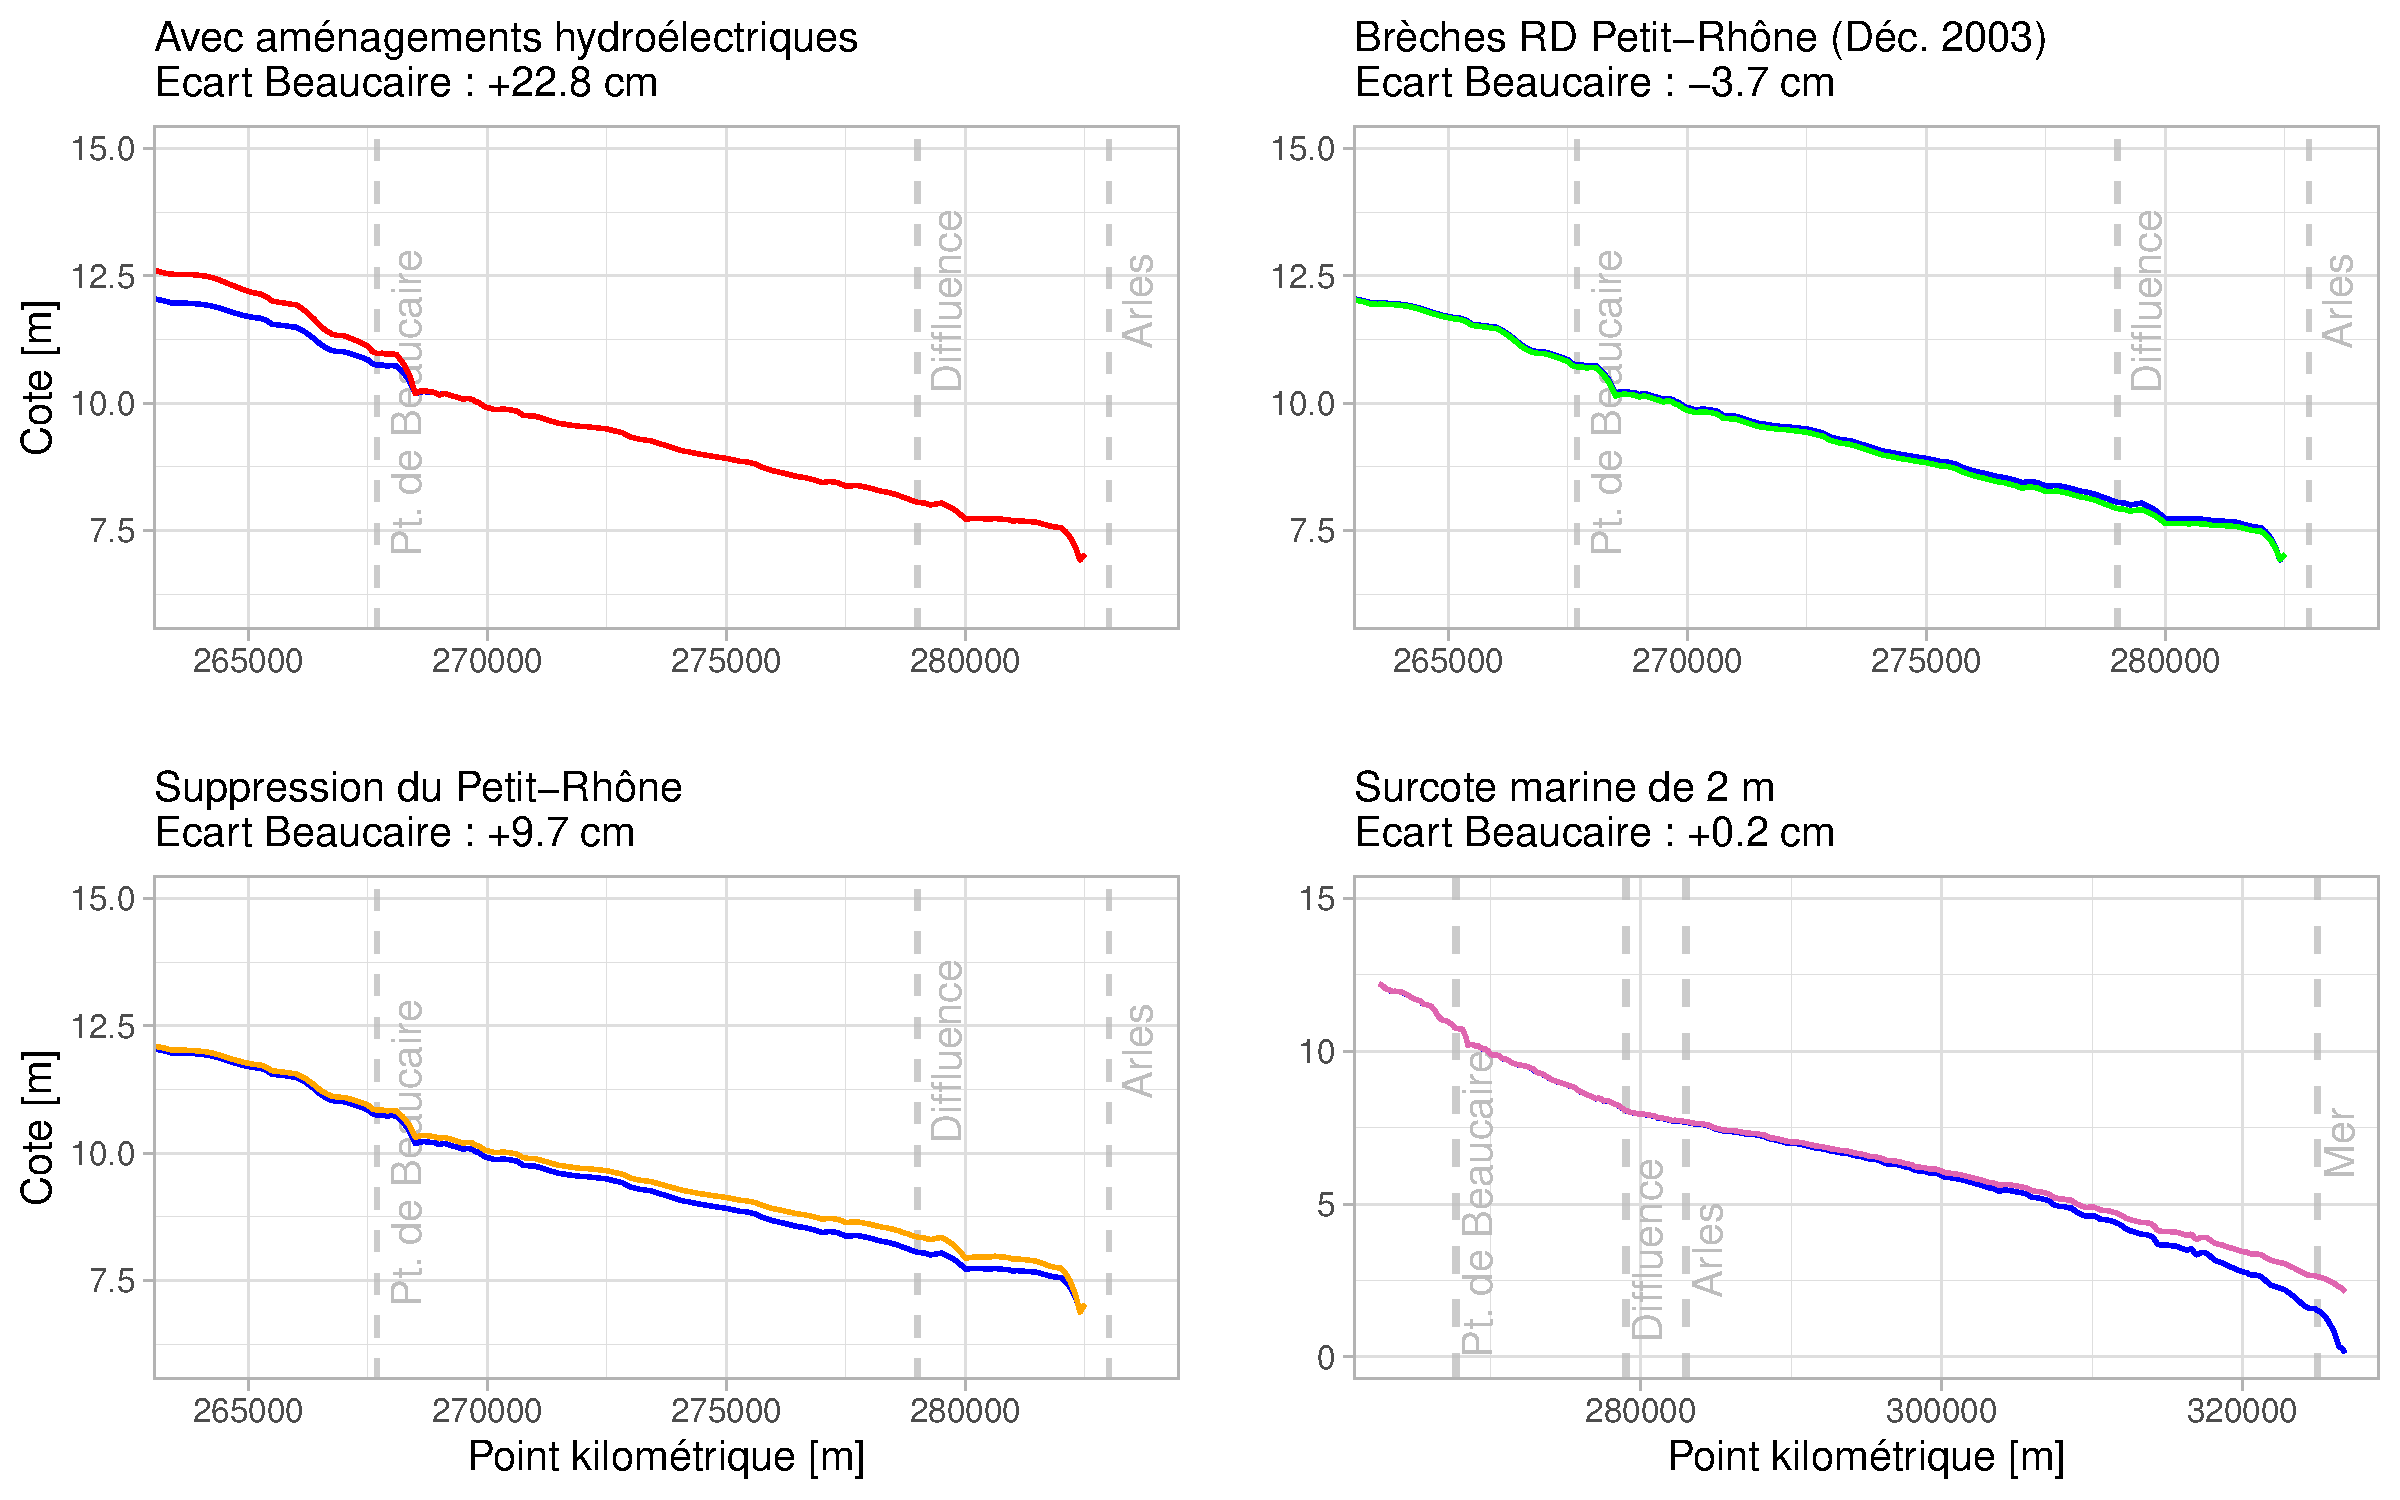
\includegraphics[width=\linewidth]{Chapitre2/Figures/4cases.pdf}
        \caption{Lignes d'eau modélisées pour 4 scénarios, comparées à la référence (bleu), pour une crue centennale en régime stationnaire. Il s'agit des lignes d'eau des biefs Vieux Rhône-Beaucaire, Beaucaire-Diffluence, Diffluence-Arles (Grand-Rhône), excepté pour le graphique du coin inférieur droit dont le dernier bief représente le Petit-Rhône (Diffluence-Mer).}
		\label{fig:Sensib4}
	\end{figure}		
		
	\subsubsection{Sensibilité à la suppression du Petit-Rhône} 
	
	\paragraph{} La morphologie du Petit-Rhône a profondément évolué au cours des derniers siècles (figure \ref{fig:Embouch}), comme souligné par \citet{pichard_les_2014} et \citet{raccasi_mutations_2008}. De plus, la part de débit correspondant au Petit-Rhône par rapport à celle du Rhône total a probablement changé au gré de ses évolutions morphologiques. Ces changements rendent complexe la reconstitution de la morphologie historique du Petit-Rhône. Afin de s'affranchir de ces reconstitutions, la solution la plus simple et la plus radicale est la suppression du Petit-Rhône du modèle hydraulique, la totalité des débits transitant alors par le bief du Grand-Rhône. On constate sur la figure \ref{fig:Sensib4} que cela a pour conséquence une augmentation de la hauteur d'eau sur l'ensemble du linéaire modélisé. L'augmentation est évidemment maximale sur le bief Diffluence-Arles, et s'élève à 9.7 cm à Pont de Beaucaire pour un débit de 11~500~\textsuperscript{3}/s. Cet impact sur la ligne d'eau à Pont de Beaucaire est relativement faible. Il correspond à un écart en débit d'environ 250~m\textsuperscript{3}/s, soit une augmentation d'environ 1.5\% (d'après la courbe de tarage la plus récente déterminée au chapitre \ref{chap:ch3}). Si l'hypothèse extrême de la suppression du Petit-Rhône n'a qu'un impact très limité sur la hauteur d'eau à Beaucaire, alors la non prise en compte des évolutions morphologiques historiques du Petit-Rhône a probablement un impact encore plus limité. La solution la plus évidente est donc la conservation Petit-Rhône dans le modèle sous sa forme moderne, soit la bathymétrie utilisée dans le modèle Rhône OSR.
	
	\subsubsection{Sensibilité aux ruptures de digues sur le Petit-Rhône}
	
	\paragraph{} De nombreuses crues ont provoqué des ruptures de digues dans l'histoire du bas-Rhône \citep{pichard_sept_2014}, notamment en 2003 \citep{medd_debit_2005}. La reconstitution de ces ruptures de digues pour les crues historiques est complexe, notamment en ce qui concerne la largeur et la profondeur de la rupture. L'importance de la prise en compte des ruptures de digues dans le modèle est étudiée en reproduisant les brèches observés en 2003 sur le Petit-Rhône. Plusieurs brèches dans les digues sont survenues pendant cet événement et sont résumées dans le tableau \ref{fig:Breches2003} tiré de l'étude du \citet{symadrem_programme_2012}. Dans cette étude, l'impact des brèches des trémies du Mas Tessier et des Ségonnaux (bief Beaucaire-Diffluence) sur la ligne d'eau a Beaucaire à été jugé faible. Seules les brèches du Petit-Rhône (Mas d'Argence et Claire Farine) seront donc reproduites ici. Ces deux brèches sont représentées par des déversements vers l'extérieur du modèle dont la profondeur et la largeur proviennent des informations présentées dans le tableau \ref{fig:Breches2003}. Les brèches sont supposées actives tout au long de la simulation, la prise en compte de leur dynamique temporelle n'ayant pas de sens dans le cadre d'une simulation en régime permanent. On constate sur la figure \ref{fig:Sensib4} que l'impact des brèches du Petit-Rhône est faible, et qu'il est maximal à proximité de la diffluence. La hauteur d'eau à Pont de Beaucaire est 3.7~cm plus basse que pour la simulation de référence, pour un débit de 11~500~\textsuperscript{3}/s. Cela représente une différence en débit de 72~m\textsuperscript{3}/s, soit une erreur d'environ 0.5\% d'après la courbe de tarage la plus récente (élaborée au chapitre \ref{chap:ch3}). Cet écart très faible indique que la considération de ce type de brèche a un impact très limité à Beaucaire. Des conclusions différentes auraient pu être tirées dans le cas de brèches apparaissant à l'aval ou à l'amont immédiat de Beaucaire. De plus, ce résultat n'est pas réellement représentatif de l'impact des brèches sur la dynamique de la crue, par exemple dans le cas d'une brèche significative survenant pendant la montée de la crue pouvant avoir un effet d'écrêtage. Dans le cas de la reconstitution du débit des crues historiques, cela pourrait conduire à une sous-estimation de ce débit pour une hauteur donnée. Cependant, la reproduction d'un tel événement n'est pas possible pour une simulation en régime permanent.
	
	\begin{figure}[h]
		\centering
		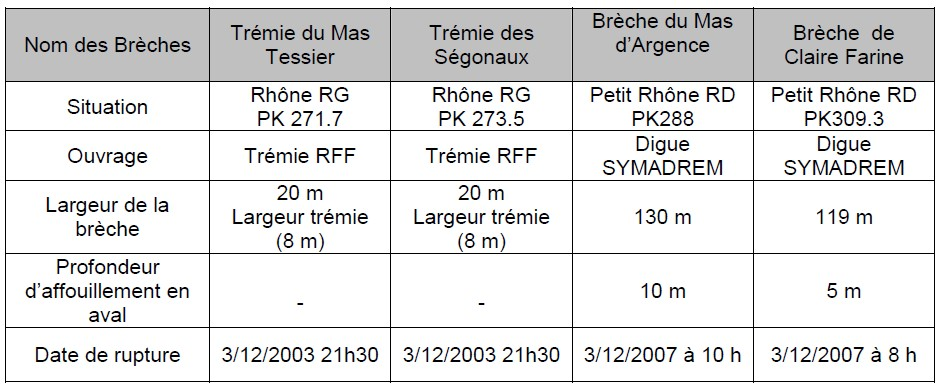
\includegraphics[width=.7\linewidth]{Chapitre2/Figures/Breches2003.jpg}
        \caption{Caractéristiques des brèches dans les digues lors de la crue de décembre 2003. Tableau tiré de l'étude du \citet{symadrem_programme_2012}.}
		\label{fig:Breches2003}
	\end{figure}		

\FloatBarrier	
	
	\subsubsection{Sensibilité aux surcotes marines}	
	
	\paragraph{} Les surcotes marines sont fréquentes en Méditerranée lors de conditions météorologiques telles que les tempêtes ou les fortes dépressions. Dans de nombreux témoignages historiques, des crues du bas-Rhône sont associées à des tempêtes maritimes \citep{pichard_sept_2014}. Ces augmentations périodiques du niveau de la mer peuvent avoir une influence sur les niveaux d'eau du Rhône. Cet impact est étudié en augmentant artificiellement le niveau de la mer en condition limite aval du modèle pour le bief du Petit-Rhône. La limite aval pour le bief du Grand-Rhône, située à Arles, n'est pas modifiée dans ce scénario. On suppose une surcote marine centennale, estimée à +2~m par \citet{kergadallan_estimation_2015}. On constate dans la figure \ref{fig:Sensib4} que l'impact de la surcote est maximal au niveau de la mer et décroit vers l'amont. Cet impact semble important sur le bief du Petit-Rhône, mais la différence de hauteur d'eau à Pont de Beaucaire n'est que de +0.2~cm pour un débit de 11~500~\textsuperscript{3}/s. Cela représente une différence en débit de 23 m\textsuperscript{3}/s, soit une erreur d'environ 0.15\% d'après la courbe de tarage la plus récente élaborée au chapitre \ref{chap:ch3}. Suite à ce constat, il ne semble pas pertinent de considérer les surcotes marines pour la modélisation des crues historiques à Beaucaire. Cependant, ce scénario suppose que la hauteur d'eau en crue à Arles n'est pas impactée par la surcote marine, ce qui est peu probable. Ce scénario pourrait être plus amplement exploré en estimant un ordre de grandeur de la différence de hauteur d'eau engendrée à Arles dans le cas d'un événement de surcote marine observé par le passé. De plus, des simulations similaires pourraient être réalisées pour représenter l'impact des embâcles causées par des arbres ou des glaces flottantes comme cela est parfois le cas pour les crues historiques de la base HISTRHÔNE.
	\FloatBarrier
	\subsubsection{Conclusions sur la simplification du modèle}
	
	\paragraph{} Les quatre scénarios présentés précédemment représentent une analyse de sensibilité sommaire afin d'identifier l'impact de quelques hypothèses simplificatrices sur la ligne d'eau à Beaucaire pour un débit constant correspondant au débit de pointe de la crue centennale de décembre 2003. Il s'agit de réduire au maximum la complexité du modèle afin de le rendre utilisable pour la simulation de crues historiques pour lesquelles les données sont rares. Il faut noter que même si l'impact de chacune de ces hypothèses simplificatrices est relativement faible, l'impact cumulé de plusieurs d'entre elles peut en revanche être significatif. Par exemple, on peut imaginer le cas d'une crue pour laquelle des brèches dans les digues ont été observées mais dont la taille n'est pas connue, et pour laquelle une surcote marine d'une amplitude inconnue a été observée. D'autres facteurs engendrent une incertitude importante des débits modélisés mais ne sont pas inhérents à la simplification du modèle. On peut notamment penser aux effets d'hystérésis dont l'impact sur les stations hydrométriques françaises a été explorée par \cite{perret_framework_2022}, mais également à la complexité d'estimer des apports du Gardon ainsi que les phénomènes de laminages au niveau de la confluence \citep{symadrem_programme_2012}. Plus intuitivement, on peut aussi penser aux incertitudes liées à la reconstitution des géométries et des rugosités historiques.
	
	\subsection{Bathymétries et topographies anciennes}
	
	\paragraph{} Une des principales limites de la modélisation des crues anciennes provient de la reconstitution de la géométrie des sections en travers. Les nombreuses évolutions morphologiques de la basse vallée du Rhône décrites pour les deux derniers siècles par \citet{raccasi_mutations_2008}, et pour les sept derniers	par \citet{pichard_sept_2014}, incitent à la plus grande prudence. Ces évolutions semblent a minima impacter le lit mineur et le lit moyen. Les évolutions du lit majeur semblent en revanche limitées aux conditions d'occupation et aux aménagements de protection pour les plus fortes crues. Les données bathymétriques complètes les plus anciennes correspondent aux planches cartographiques du Rhône navigable de Lyon à la mer, provenant des archives \citet{cnr_cartes_1908}, dont les mesures ont été réalisées entre 1907 et 1908 pour la zone de Beaucaire (figure \ref{fig:BathyTopo}, haut). Les relevés bathymétriques sont calés sur la ligne d'eau d'étiage de 1907-1908. Seul le chenal de navigation est représenté, ce qui peut poser problème, notamment à Beaucaire où seule la bathymétrie du chenal navigable (en rive droite à cette époque) est représentée. Il est possible de reconstituer la bathymétrie des chenaux secondaires pour les quelques sections en travers où des relevés sont disponibles autour de 1845 (figure \ref{fig:ProfGoux}), soit avant les travaux de correction de Girardon, lancés dès 1860. En ce qui concerne le lit majeur, la carte topographique du cours du Rhône (1860) est un document exceptionnel provenant des archives \citet{cnr_carte_1876}, qui présente des relevés topographiques réalisés entre 1857 et 1876, avant la grande phase d'aménagement du fleuve. Les relevés de la zone de Beaucaire ont été réalisés entre 1870 et 1876 (figure \ref{fig:BathyTopo}, bas). Des profils transversaux sont disponibles tous les kilomètres (sous réserve de parvenir à les déchiffrer) et couvrent un profil allant des limites du lit mineur jusqu'au delà des limites du lit majeur.
		
	\begin{figure}[h]
		\centering
		\begin{subfigure}{.6\linewidth}
			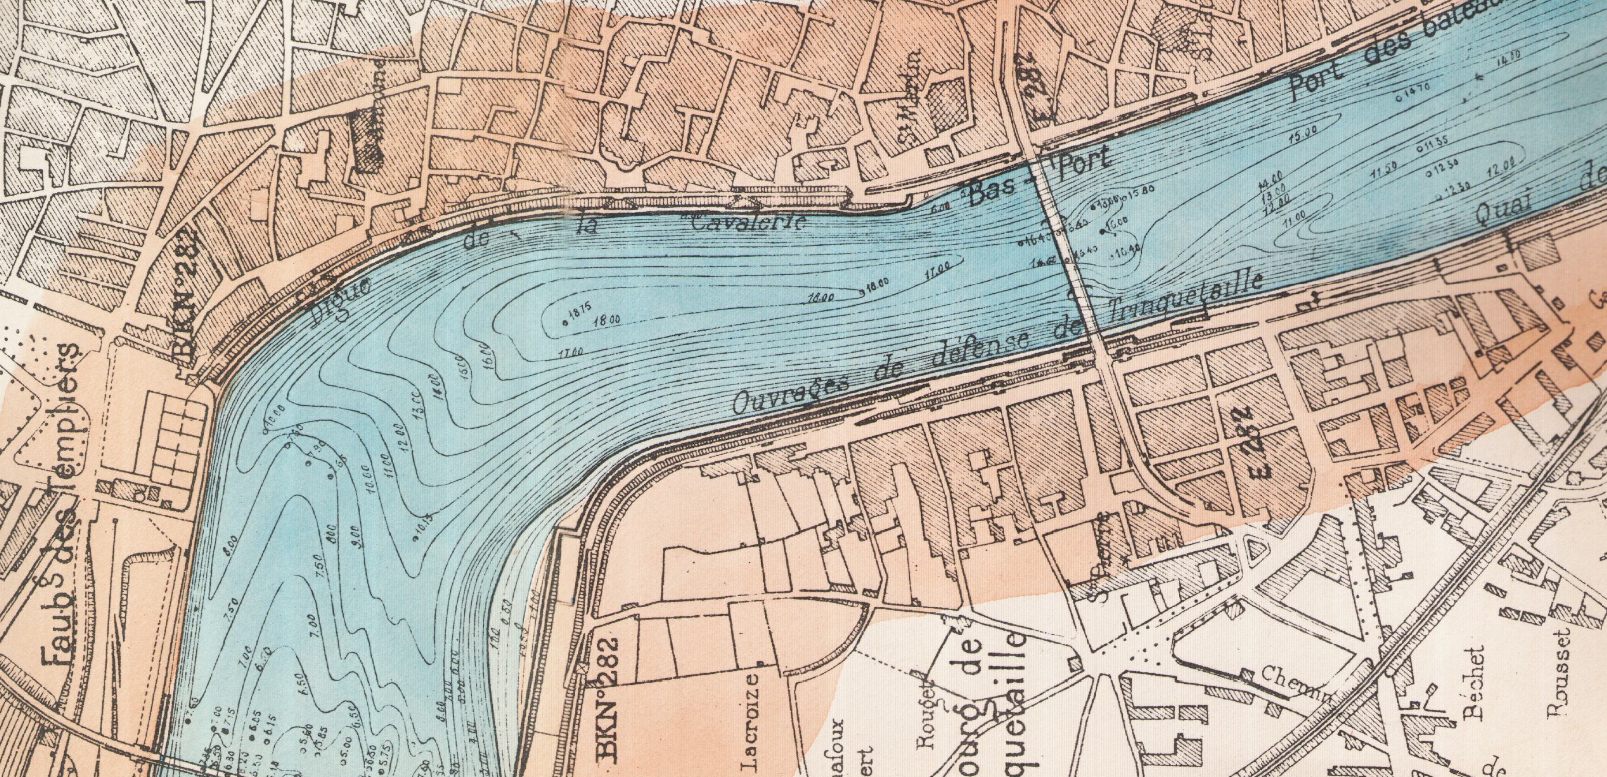
\includegraphics[width=\linewidth]{Chapitre2/Figures/BathyArles1897.png}
		\end{subfigure}
		
		\vspace{7pt}
		
		\begin{subfigure}{0.5\linewidth}
			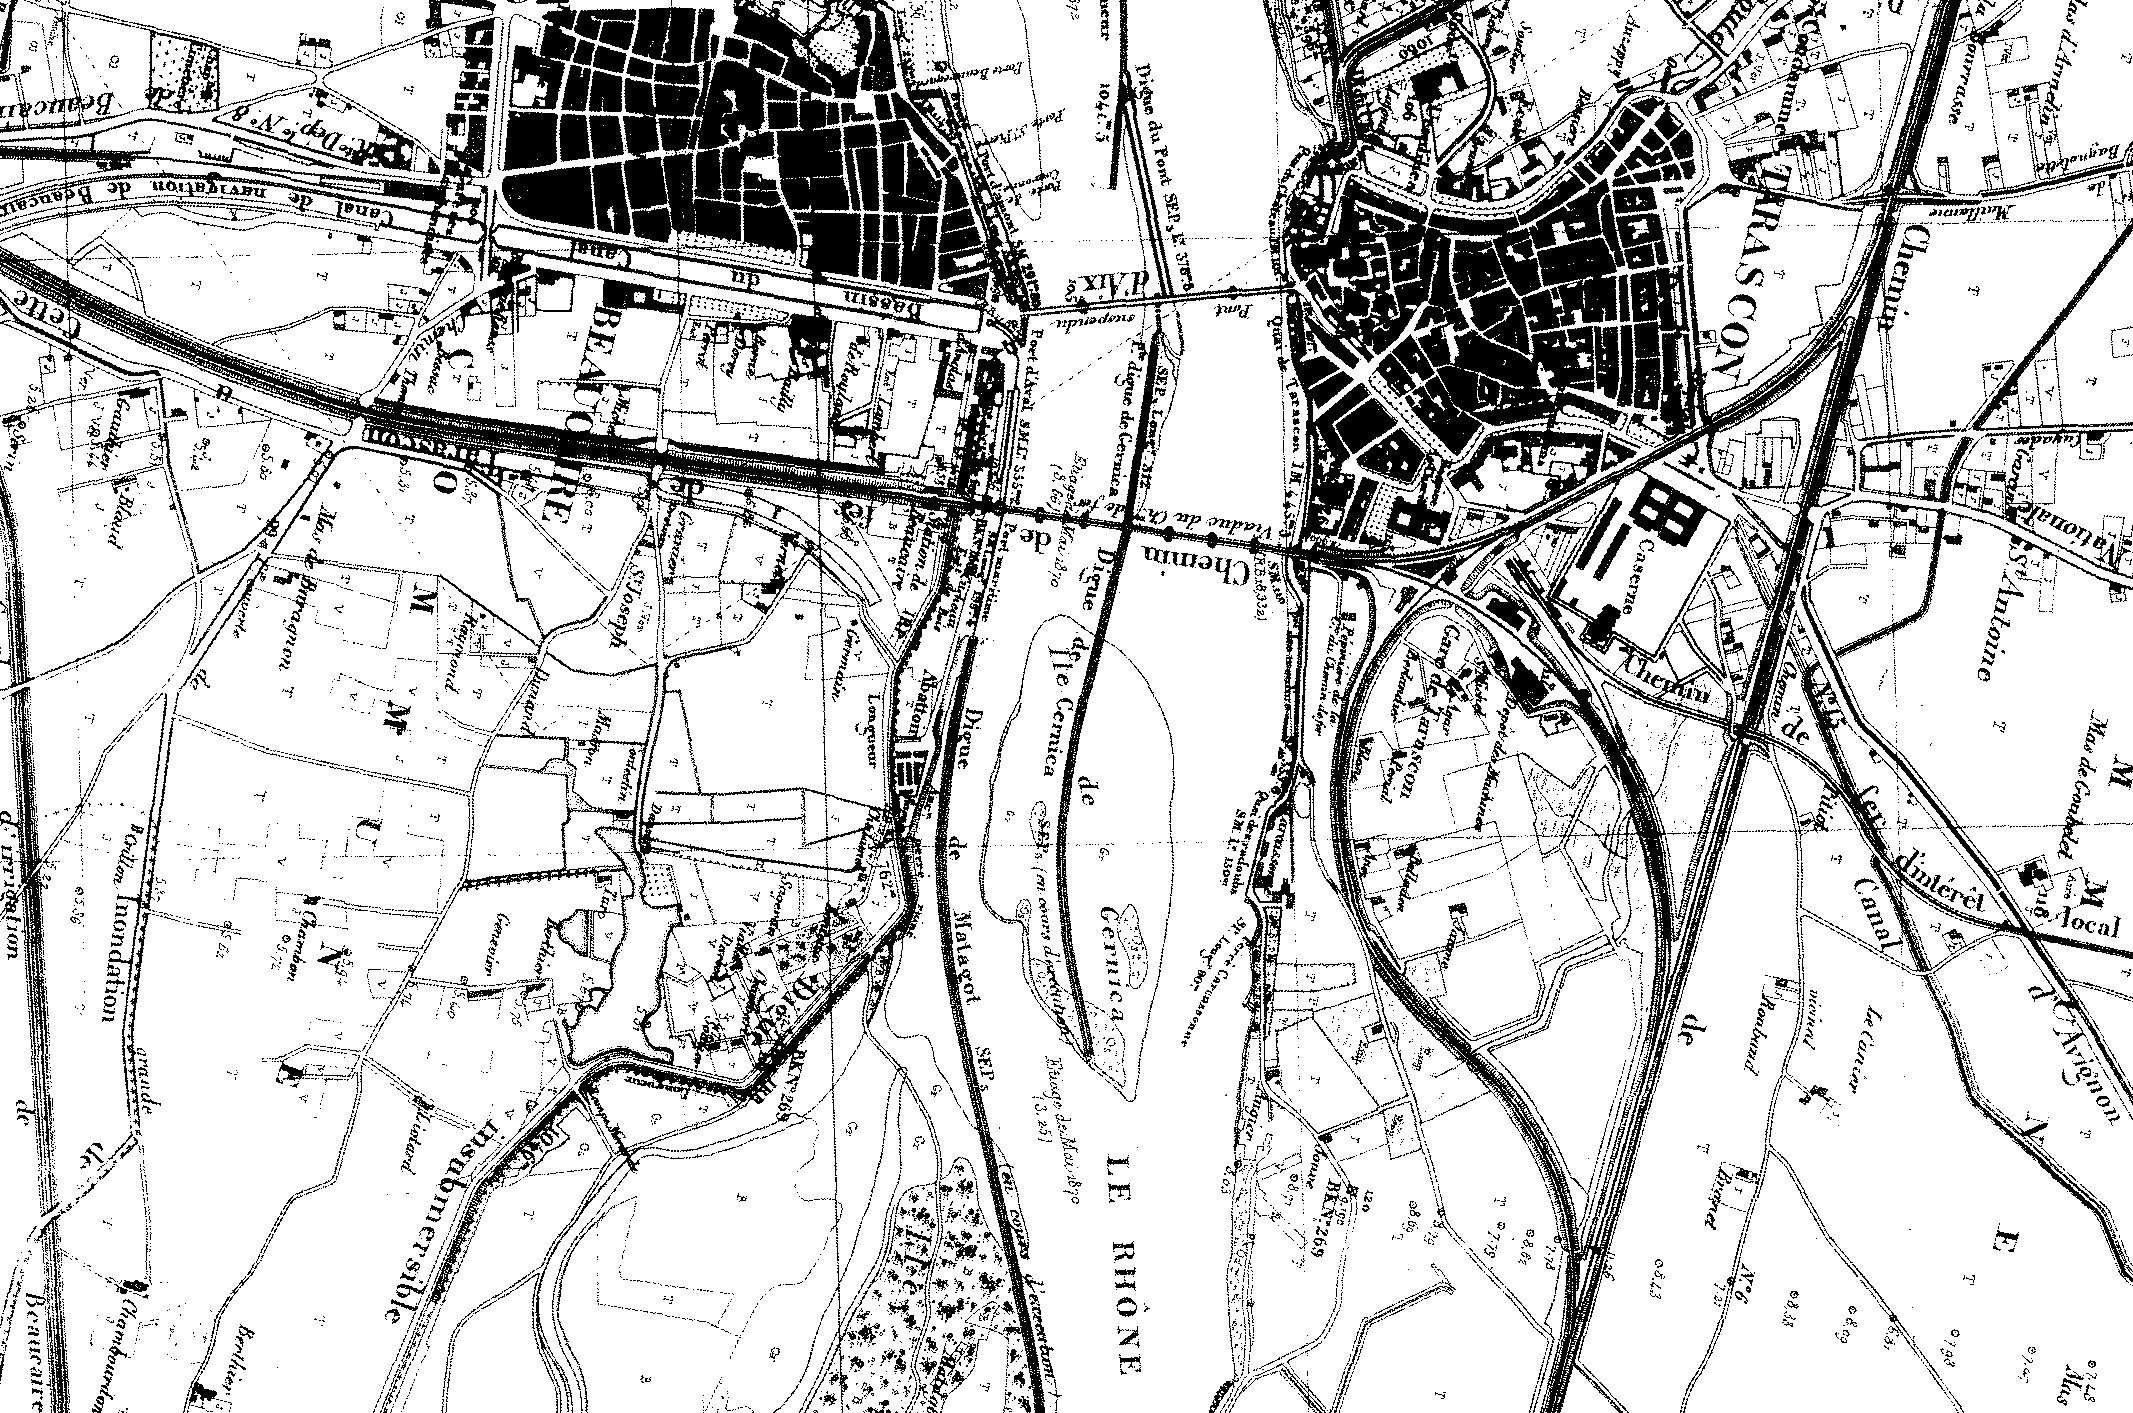
\includegraphics[width=\linewidth]{Chapitre2/Figures/Atlas1860.jpg}
		\end{subfigure}
		\caption{Haut : Carte bathymétrique du Rhône de Lyon à la mer (1897-1908) pour la zone d'Arles \citep{cnr_cartes_1908}. Les isobathes sont données par rapport à l'étiage de 1908. Les relevés couvrent seulement le chenal navigable du Rhône. Bas : Carte topographique du Rhône (1860) pour la zone de Beaucaire-Tarascon \citep{cnr_carte_1876}. Pour chaque point kilométrique, un profil en travers est disponible (en bas à droite).}
		\label{fig:BathyTopo}
	\end{figure}
	
	\paragraph{} En résumé, les plus anciennes données topographiques et bathymétriques disponibles en basse vallée du Rhône remontent au milieu du XIX\textsuperscript{ème} siècle. La modélisation des crues antérieures aux relevés limnimétriques (débutant en 1816) de la base HISTRHÔNE devra donc s'appuyer sur ces données faute de mieux. De fortes hypothèses quant à la morphologie du lit mineur (et dans une moindre mesure du lit majeur) devront être faites. Il sera par exemple possible de simuler un enfoncement ou un exhaussement de la totalité du lit majeur au sein du modèle. 
	
\FloatBarrier	
	
	\subsection{Recensement des informations nécessaires à la modélisation hydraulique} 
	
	\paragraph{} Des informations jugées utiles à la modélisation ont été extraites de la base HISTHRÔNE pour les crues de la catégorie C4 de 1353 à 1840. Elles sont présentées dans l'annexe \ref{sec:TabC4} sous la forme d'un tableau. Chacune des crues est succinctement décrite (zone inondée, causes probables, etc.) et les informations jugées nécessaires à la modélisation sont renseignées. Ces informations sont très diverses : réaction des affluents, hauteurs aux échelles reconstituées, mentions de hauteurs d'eau hors échelle limnimétrique, dégâts aux digues de protections, etc. Pour certaines crues, les informations disponibles semblent parfois suffisantes pour en estimer le débit via la modélisation hydraulique. Ce n'est pas toujours le cas. Ces divers niveaux d'information disponibles dans la base HISTRHÔNE sont explorés via les exemples suivants. 
	
	\paragraph{} L'inondation de 1745 est due à trois crues successives dont la première était la plus forte le 4 novembre. «\textit{Les pluyes abondantes et continuelles des 4,5,6,7 Novembre 1745 ayant inondé tout le terroir de cette ville et celui des villes voisines, la roubine du Vigueirat ne pouvant contenir ses eaux rompit et versa en divers quartiers de Trébon, les eaux du Rhône vinrent sur le quai, la chaussée du Trébon rompit à demi quart de lieue de la ville […]}» (source : Notes historiques sur Arles, BM Arles). La hauteur à l'échelle reconstituée de Véran à Arles est de 5.31 m et de nombreuses informations de hauteurs d'eau hors échelle sont également disponibles : «\textit{2.5 m d'eau dans les maisons de Tarascon où le Rhône entrait par la porte du château}»; «\textit{Tarascon est en partie sous 10 pieds [3,25 m] d'eau et il y a 10 à 12 pieds d'eau dans la plupart des maisons}»; «\textit{[3.5 m] d'eau sur le Pont de Crau}». Les digues ont connu de nombreux dégâts qui sont rapportés avec précision : «\textit{Brèche de [60 m] de large à la chaussée du Trébon à [500 m] d'Arles}»; «\textit{[600 m] d'ouvertures au pas du bouquet [Tarascon]}»;«\textit{Rupture de la roubine du Vigueyrat [Arles]}»; «\textit{Chaussée de Camargue rompue en plusieurs endroits du côté du Baron}»; «\textit{Il semble que les premiers débordements proviennent du canal du Vigueirat, qui inonda le Trébon, avant la rupture des chaussées en ce même quartier, à un demi quart de lieue [environ 600 m] de la ville [probablement près de l'actuelle gare d’Arles]}». De plus, on peut noter que «\textit{le rhone a diminué de 10 pieds d'un coup, certainement suite aux ruptures de digues à Tarascon}». Ainsi, moyennant quelques hypothèses sur la hauteur des brèches faites aux digues de protection, il semble possible de modéliser le débit de cette crue à l'aide des nombreuses hauteurs d'eau disponibles aux échelles et en dehors. 

	\paragraph{} Dans d'autres cas, bien que des informations de hauteur d'eau soient disponibles, des brèches aux digues sont mentionnées à plusieurs reprises mais leur longueur n'est pas connue, ce qui peut compliquer l'estimation du débit. On peut par exemple citer le cas de la crue de décembre 1755 qui est décrite comme étant la crue la plus importante du XVIII\textsuperscript{ème} siècle. La crue atteint 5.47 m à l'échelle Véran d'Arles. Des hauteurs hors échelle sont également disponibles : 2.6 m dans la plaine de Beaucaire; 2 m d'eau dans les maisons du quartier Notre Dame de Bonne Aventure à Tarascon; 2.75 m dans les maisons à coté de la porte St Jean; etc. Cependant, les informations concernant les brèches sont sporadiques : «\textit{Brèche à la chaussée d'Argence, les eaux remontent jusqu'à environ 12 km dans le terroir}». L'estimation d'un débit dans ces conditions est donc relativement incertaine.
  	
	\paragraph{} Enfin, d'autres crues semblent complètement inexploitables, en l'absence de données de hauteur fiables. Par exemple, pour la crue dite «\textit{extraordinaire}» de 1573, aucune hauteur n'est disponible, que ce soit aux échelles reconstituée ou en dehors. En revanche de nombreuses ruptures de digues sont mentionnées : «\textit{Vers Beaucaire, plus de [6 km] de chaussées ruinées. Dont 25 cannes à la Bergantière, 500 cannes au dessus du port ne autre au trou du Sauze}». 
	
	\paragraph{} On peut également relever des cas très particuliers, comme la crue de 1674, initiée par la Durance les 15 et 16 novembre. Au cours de cet événement, «\textit{les eaux de la Durance se jettent en partie dans le Trébon par le débouché de Saint-Gabriel}» (près de Tarascon). Cette avulsion représente un changement morphologique majeur. La modélisation du débit de cet événement en l'absence de données plus précises que des seuls témoignages semble dans ce cas inespérée.	
	
	\paragraph{} Suite à cet état des lieux, il semble complexe de pouvoir modéliser le débit de chacune des crues C4 de la base avec un même modèle hydraulique. De plus on constate de grandes disparités entre les informations disponibles d'une crue à l'autre, ainsi que des changements morphologiques majeurs pour certains événements. Chacune des crues mériterait une analyse détaillée ainsi qu'une adaptation du modèle hydraulique. Aussi, d'importantes incertitudes semblent entourer cet exercice. Il faut également noter que dans ce contexte, la quantification des incertitudes de modélisation semble particulièrement complexe. La question de la faisabilité de ces reconstitutions devant le temps limité de la thèse s'est donc posée. La plus value de ces estimations de débit semble faible alors que cet exercice est très chronophage et incertain. Sachant qu'il est possible d'intégrer ces événements à l'analyse fréquentielle des crues en utilisant la seule information du nombre de dépassements d'un seuil de perception, la modélisation hydraulique du débit des crues C4 est abandonnée. En revanche, les événements historiques présentés ci-dessus et dans l'annexe \ref{sec:TabC4} seront utilisés sous forme d'occurrences supérieures à un seuil de perception. 
	
	\epigraph{«\textit{Je ne dirais pas que c'est un échec. Ça n'a pas marché.}»}{Emmanuel Macron le 14 octobre 2020}
		
	\FloatBarrier	
	\subsection{Limites et perspectives pour la modélisation hydraulique des événements historiques}
	
	\paragraph{} Les travaux décrits dans cette section n'ont pas permis, dans le temps limité de la thèse, d'estimer le débit des événements anciens à l'aide de la modélisation hydraulique. Cependant, ils ont permis de dresser un bilan des données disponibles à cet effet, ainsi que d'en identifier les limites. L'impact de plusieurs hypothèses permettant une simplification du modèle hydraulique a également été exploré dans le but de pouvoir effectuer des modélisations avec une quantité minimale de données d'entrée. Les idées développées dans les lignes suivantes ont pour but de définir les contours et les limites à garder en tête dans l'optique de poursuivre ce travail d'estimation du débit des événements historiques à Beaucaire.
	
	\paragraph{} Pour commencer, la limite amont du modèle a été définie à l'aval immédiat de la confluence avec la Durance, ce qui permet d'éviter l'estimation du débit de cet affluent. Cependant, il reste à définir une solution pour la confluence du Gardon. Dans le modèle présenté dans cette section, celui-ci était représenté par un apport latéral, mais l'estimation du débit de cet apport est impossible dans le cas d'événements historiques. Une des possibilités pour contourner ce problème serait de fixer la limite amont du modèle à l'aval immédiat de la confluence avec le Gardon. Il faut garder à l'esprit que la morphologie historique de cette confluence est plus simple que la morphologie actuelle, le Gardon se jetant dans le Vieux-Rhône et n'ayant pas d'influence sur le débit du chenal de dérivation. Ensuite, la reproduction dans le modèle des deux chenaux présents à Beaucaire (qui communiquent à haut débit) est un obstacle conséquent pour la modélisation 1D car il est complexe de modéliser leur communication à haut débit. Seule la modélisation 2D peut permettre de reproduire ce phénomène de manière convenable, mais elle nécessite une quantité d'informations plus importante. Il semble donc nécessaire, dans un but de simplification, de fixer la limite amont du modèle à l'amont de la division du Rhône en deux bras. 
	
	\paragraph{} En ce qui concerne la limite aval, la conservation du Petit-Rhône jusqu'à la mer dans son état actuel semble être la solution la plus évidente et la moins couteuse en termes de données pour garantir une extraction cohérente des débits du Rhône. La limite aval du Grand-Rhône fixée à Arles semble également être la meilleure solution compte tenu des niveaux reconstitués par Véran à l'échelle du port \citep{pichard_les_1995}. Pour 10 des 18 crues C4 de 1300 à 1810, une estimation de la hauteur à Arles est disponible (voir annexe \ref{sec:TabC4}). La modélisation semble en revanche plus complexe pour les 8 autres crues, pour lesquelles la limite aval pourra par exemple être fixée au niveau de la mer, des reconstitutions historiques du niveau marin étant probablement disponibles.
	
	\paragraph{} En ce qui concerne la géométrie du Rhône en entrée du modèle, les données topographiques et bathymétriques disponibles ne permettent pas de remonter à une époque plus ancienne que le milieu du XIX\textsuperscript{ème} siècle. Les conditions d'écoulement pré-1816 sont méconnues bien que des cartes anciennes et assez approximatives existent (par exemple, la carte de Bompar datant de la fin du XVI\textsuperscript{ème} siècle). Il s'agit par exemple de la carte de Cassini datant du XVIII\textsuperscript{ème} siècles ou des cartes présentées par \citet{pichard_sept_2014}. Des hypothèses grossières pourront être faites sur les bathymétriques des périodes anciennes, par exemple en exhaussant ou en enfonçant artificiellement le lit mineur dans le modèle hydraulique, suivant les constatations de \citet{pichard_sept_2014} ou d'autres études de la géomorphologie ancienne du Rhône. Cette méconnaissance de la morphologie du Rhône avant 1800 est la plus grosse inconnue autour des reconstitutions des débits anciens.
	
	\paragraph{} Dans les premiers essais de modélisation présentés dans ce chapitre, le calage de la rugosité du chenal du modèle OSR a été conservé, bien que celui-ci ne soit pas adapté à un contexte de crue. Ce calage pourrait être revu, une fois les profils en travers du modèle revus sur la base des topographies et bathymétries du XIX\textsuperscript{ème} siècle. La reproduction de la crue de 1856 pourrait être une première étape de ce calage, des lignes d'eau de cet événement étant disponibles dans les archives CNR. Cependant, les coefficients de rugosité de 1856 ne sont probablement pas valables pour les crues antérieures au XIX\textsuperscript{ème} siècle. Il semble complexe d'adapter ces coefficients sur la base de l'occupation des sols pré-XIX\textsuperscript{ème} siècle, les données cartographiques de cette période étant rares et imprécises. 
	
	\paragraph{} En résumé, de nombreuses incertitudes entourent l'estimation du débit des crues anciennes. Ces incertitudes proviennent notamment des données d'entrée, mais également du modèle lui-même qui représente une représentation très simplifiée de la réalité des écoulements historiques. Voici une liste non exhaustive de ces différentes incertitudes :
	
	\begin{itemize}
		\item La reconstitution imprécise des sections en travers historiques du Rhône, basée sur des bathymétries plus récentes (XIX\textsuperscript{ème} siècle) que les crues de la base HISTRHÔNE.
		\item L'incertitude des niveaux exacts atteints par les crues que les témoignages anciens ne reflètent pas parfaitement. En effet, de nombreuses informations sur les zones impactées par les crues sont disponibles, mais celles-ci ne mentionnent que rarement la profondeur maximale atteinte.
		\item  L'existence de brèches dans les digues qui, bien que souvent mentionnées dans les écrits, ne permettent pas de reconstituer la largeur et la profondeur de ces brèches, ainsi que leur évolution au cours de la crue.
		\item L'incertitude autour de la dynamique de la crue qu'il est impossible de connaitre en l'absence de mesures continues.
		\item La connaissance imparfaite des conditions aux limites du modèle, tel que le niveau de la mer Méditerranée pour le bief du Petit-Rhône, qu'il est impossible de connaitre pour les crues du XIV\textsuperscript{ème} siècle.
		\item Les coefficients de rugosité du modèle, qu'il est complexe d'estimer compte tenu de la méconnaissance de l'occupation des sols et de leur nature pour les périodes anciennes.	
	\end{itemize}
		
	\paragraph{} La quantification de l'incertitude des débits estimés est nécessaire mais semble complexe. Elle pourra par exemple passer par des hypothèses hautes et basses sur les différents points listés ci-dessus. Un autre moyen plus complexe et couteux en temps de calcul consiste à élaborer un algorithme Monte Carlo couplé au modèle hydraulique permettant de propager l'ensemble des incertitudes au résultat final.	
	

\FloatBarrier
\section{Conclusion du chapitre}

	\paragraph{} Une chronique limnimétrique continue exceptionnellement longue est disponible à Beaucaire : 205 années entre 1816 et 2020, avec seulement une lacune au moment du changement de station de 1967 à 1970. La station de Beaucaire est d'une grande importance car elle est la station du Rhône "complet" la plus à l'aval du bassin versant. Elle enregistre donc la grande complexité des très divers apports du Rhône. L'échelle limnimétrique du Pont de Beaucaire n'a supposément jamais été déplacée depuis son installation en 1816. Elle fut donc le témoin des nombreux changements naturels et anthropiques du chenal : des digues de protection contre les inondations, jusqu'aux aménagements en lit mineur pour favoriser la navigation, en passant par l'installation d'aménagements hydroélectriques. L'installation de ces derniers en 1970 a nécessité le déplacement de la station quelques centaines de mètres plus à l'aval. Ce riche historique limnimétrique peut permettre la reconstitution d'une chronique de débits de plus de deux siècles, à condition de prendre en compte les nombreuses évolutions du chenal compilées dans ce chapitre lors de l'élaboration des courbes de tarage. De plus, à l'image des travaux de \citet{bard_actualisation_2018}, une prise en compte des nombreuses sources d'incertitude sera nécessaire. 
	
	\paragraph{} La reconstitution de deux siècles de débit en continu semble envisageable suite au bilan des données hydrométriques disponibles. Cependant, il faudra veiller à l'homogénéité de la chronique reconstituée. Contrairement à certains fleuves européens, le Rhône n'a pas connu de dérivations ou de travaux majeurs, mis à part le canal de Savières près de Chambéry, avec un impact négligeable à Beaucaire. Cependant, plusieurs autres facteurs peuvent impacter cette homogénéité, et notamment l'installation d'aménagements en lit mineur qui peuvent modifier la dynamique des crues. Afin de quantifier cet impact, l'évolution du temps de propagation des crues au fil de l'installation des différents aménagements en lit mineur a été étudiée. Les temps de propagation entre Lyon et Beaucaire de 121 crues non-débordantes de type océanique ont été compilés suite à l'analyse des limnigrammes. Il apparait que le temps de propagation de ce type de crues a progressivement diminué au cours des différentes phases d'aménagement et est passé d'environ 48 h en 1840 à environ 16 h de nos jours. La modélisation hydraulique d'un événement océanique type dans le contexte actuel à permis d'obtenir un temps de propagation de 18 h, ce qui confirme la valeur de 16 h estimée à l'aide des limnigrammes. Les aménagements en lit mineur ont probablement d'autres conséquences, notamment sur la forme des hydrogrammes de crue, le débit de pointe, ou la concomitance des crues du Rhône avec celles de ses affluents. Ces évolutions devront êtres gardées à l'esprit lors de l'évaluation de l'homogénéité des échantillons de crues préalable à l'analyse fréquentielle lors des chapitres suivants. L'impact de ces aménagements sur les temps de propagation de crues plus importantes, ou dans le cas de crues cévenoles ou généralisées n'a pas été étudié ici mais pourrait également être intéressant.
	
	\paragraph{} En plus du riche passé en termes de relevés limnimétriques, la basse vallée du Rhône, par son histoire religieuse et culturelle, regorge de documents qui témoignent de son histoire hydroclimatique. Ces éléments historiques ont été récoltés et mis à disposition dans la base de données HISTHRÔNE (\url{histrhone.cerege.fr}) à la faveur d'un très important travail d'archives \citep{pichard_sept_2014}. Ce sont ainsi plus de 1500 événements depuis le XIII\textsuperscript{ème} siècle que décrivent ces divers documents et témoignages. Les crues étant des événements marquants pour les populations ripariennes, elles sont nombreuses dans la base de données, où elles sont classées selon les dommages engendrés. Une estimation de l'ordre de grandeur du débit de ces catégories a été effectuée en se basant sur une comparaison des crues récentes avec les hydrogrammes de Beaucaire. Ces estimations pourront permettre l'utilisation des crues antérieures aux enregistrements continus pour l'analyse fréquentielle à condition de considérer un seuil de perception dont le débit n'est pas parfaitement connu. De plus, des probables fluctuations de la vulnérabilité des populations aux inondations ont été mises en évidence et peuvent compliquer l'utilisation des seules mentions de crues pour l'analyse fréquentielle en l'absence d'estimations de débit pour chacun des événements. 

	\paragraph{} La piste de la modélisation hydraulique pour l'estimation du débit des crues historiques a été explorée. Le modèle MAGE OSR 1D utilisé pour étudier la dynamique sédimentaire du Rhône du Lac Léman à la mer a été adapté à l'étude des crues du bas Rhône. Étant donné la complexité de reconstituer la morphologie et la bathymétrie du Rhône avant le XIX\textsuperscript{ème} siècle, la sensibilité du modèle à plusieurs hypothèses simplificatrices a été explorée afin d'en réduire la complexité. Il apparait notamment de ces tests que la meilleure configuration semble être de considérer comme limite aval du modèle côté Grand-Rhône la ville d'Arles, où la hauteur d'eau de nombreuses crues historiques est disponible \citep{pichard_hauteurs_2013}. La fixation de la limite aval du Petit-Rhône à son embouchure semble être la solution la plus pratique en l'absence d'enregistrements de hauteur des crues historiques sur ce bief. Il sera cependant complexe de reconstituer la bathymétrie de ce bief dont la morphologie a grandement évolué au cours de l'histoire. Par la suite, l'impact de différents scénarios sur la ligne d'eau à Beaucaire a été exploré : la présence d'aménagements hydroélectriques, la présence de brèches dans les digues du Petit-Rhône (scénario de la crue de 2003), l'évolution morphologique du Petit-Rhône (et l'hypothèse extrême de sa suppression du modèle), la présence d'une surcote marine pendant la crue. Il apparait que parmi ces quatre scénarios, seule la considération des aménagements hydroélectriques a un impact significatif sur la ligne d'eau à Beaucaire. Cependant, des perturbations apparaissant dans des zones plus proches de la station de Beaucaire n'ont pas été modélisées mais pourraient avoir un impact plus important.
	
	\paragraph{}	 Au-delà de ces différents scénarios de simplification du modèle, plusieurs limites à la reconstitution du débit des crues anciennes persistent et ont été listées. La principale limite étant la reconstitution des sections en travers du Rhône et de leur rugosité avant le XIX\textsuperscript{ème} siècle. En effet, les plus anciennes données disponibles remontent en 1908 pour la bathymétrie et en 1876 pour la topographie de la plaine alluviale. De plus, l'estimation de l'incertitude autour des débits modélisés semble complexe à réaliser. Au regard du temps limité de la thèse et de la possibilité d'utiliser ces données historiques pour l'analyse fréquentielle des crues sans avoir à en modéliser le débit via l'estimation d'un seuil de perception, nous avons décidé de ne pas poursuivre ces travaux. Cependant, les contours et les limites de cet exercice ont été définis, ce qui pourra être utile à qui envisagera de telles reconstitutions. 
	
	
%	\paragraph{} Le présent chapitre a permis de dresser le bilan des données de crues disponibles à Beaucaire. Tout d'abord, une chronique limnimétrique continue de 1816 à aujourd'hui est disponible, permettant l'estimation des débits de cette période via l'élaboration de courbes de tarage. L'analyse de l'évolution de la morphologie du Rhône au cours des deux derniers siècles sera utile à cet effet. Il faudra cependant porter une attention particulière à l'estimation et la propagation des diverses incertitudes provenant de la mesure de hauteur d'eau, des jaugeages, ou de l'élaboration des courbes de tarage. Les données de la base HISTRHÔNE ont ensuite permis de rassembler un nombre important d'événements de crues antérieurs à l'installation de l'échelle limnimétrique de Beaucaire (1816). Ces crues sont classées dans la base de données en différentes catégories selon les dommages engendrés. Il faudra garder à l'esprit que la vulnérabilité des populations aux crues du Rhône à pu changer au cours de l'histoire et impacter la classification des événements. Si le débit des événements anciens n'a pas pu être estimé à l'aide de la modélisation hydraulique, les limites et les contours de cet exercice ont pu être définis. Il faut garder à l'esprit que l'utilisation des données pré-enregistrements continus pour l'analyse fréquentielle des crues n'est pas conditionnée à l'estimation du débit de chacun des événements. Pour finir, l'évolution du temps de propagation des crues au cours des différentes phases d'aménagements en lit mineur a été étudiée. Il faudra s'assurer que la diminution du temps de propagation des crues mise en valeur dans ce chapitre n'a pas d'impact sur l'homogénéité des échantillons utilisés pour l'analyse fréquentielle. 

%\newpage
%
%\section{Annexe 1 : Données des crues C4 de la base HISTRHÔNE pour la modélisation hydraulique}
%\label{sec:TabC4}
%
%\begin{tiny}
%
%\begin{landscape}
%	\begin{longtable}{|p{0.4cm}|p{0.5cm}
%	 |p{0.5cm}|p{2cm}|p{0.5cm}|p{2cm}|p{1cm}|p{1cm}|p{1cm}|p{1cm}|p{1cm}|p{1cm}|p{2cm}|p{1cm}|}
%	
%    \hline
%  \textbf{Année} & \textbf{Mois} & \textbf{Modélisable } & \textbf{Description} & \textbf{Causes} & \textbf{Info affluents} & \textbf{Hauteurs échelle} & \textbf{Info hauteur Beaucaire - Tarascon} & \textbf{Info hauteur Arles} & \textbf{Info hauteur Avignon} & \textbf{Indices hauteur autre} & \textbf{Ouverture digues} & \textbf{Autres infos} \\ \hline
%        \textbf{1353} & mai & Non & Le Rhône inonde la plaine depuis Avignon jusqu’à la mer. & Gel du Rhône et de la Durance & ~ & ~ & ~ & ~ & ~ & x & ~ & ~ \\ \hline
%        \textbf{1398} & octobre & Non & Crue dévastatrice du Rhône selon les chroniques d'Avignon et de l'arlésien Bertran Boysset & ~ & ~ & ~ & ~ & ~ & ~ & inférieur de 10 cm à la crue de 1396 à Arles (qui est une C3?...) & ~ & ~ \\ \hline
%        \textbf{1433} & novembre & Oui (Avignon) & Grande inondation qui s'étend d'Avignon à la mer & Pluie et fonte des neiges (en novembre?) & Débordement conjoint Durance et Sorgue & 6,77 m au dessus de l'étiage à Avignon, échelle indéterminée et 7,08 m au pont suspendu d'Avignon & ~ & ~ & Miracle chapelle des pénitents gris, 1 m d'eau dans la nef & ~ & ~ & Toute la Carmarque est inondée, des pirates y pénètrent et se livrent à des pillages \\ \hline
%        \textbf{1471} & septembre & Non & L'une des plus grandes inondations conjuguées du Rhône et de la Durance & Probablement cévenol, caractère brutal & Durance en crue & X & ~ & ~ & une partie des murailles abattues, repère de crue église st michel de Caderousse, 1m52 au dessus du dallage & Caderousse, chapelle d'Ancezune, 1m52 au dessus du dallage & à Arles & ~ \\ \hline
%        \textbf{1529} & novembre & Oui & "Grande inondation du Rhône dit de Saint-Martin (""La Ronada de San Martin"") à Arles." & X & X & 5,25 sur l'échelle de Véran (Arles) & porte St Jean de Tarascon endommagée par la crue & Trébon, plan du bourg et camarque inondés & 300 m de remparts abattus & ~ & Levées de la chaussée du trébon endommagée (arles) & ~ \\ \hline
%        \textbf{1548} & novembre & Oui (Avignon) & Caractère foudroyant à Avignon mais peu d'échos à Beaucaire et Arles & crue à prépondérance océanique très nette, mais avec des apports duranciens et cévenols évoquant aussi des pluies méditerranéennes, limitées à un secteur étroit autour du couloir rhodanien & Débordement de la Durance à Avignon & X & Chaussées ruinées à Tarascon, murailles démolies & Hôpital St Lazare endommagé & " L'eau entre dans la ville ""jusques à la Saunerie, à Saint-Agricol, à la Croix de Lunel, à Sainte-Catherine … HR.   L'eau atteint la coquille de la chapelle St Nicolas sur le pont St benezet,   25 cm en dessous du plus haut de la porte de la Ligne,   tient toutes les arcades du pont et à environ 1m50 avant de toucher le plus haut des arcs. RAPPORT COMPLET à revoir sur des contradictions concernant les marques de crues à Avignon" & nombreux indices contradictoires à Avignon quand au dépassement par cette crue de celle de 1856. & ~ & ~ \\ \hline
%        \textbf{1570} & décembre & Hauteur seulement & Inondation générale du Rhône, concernant l'ensemble du bassin. Inondation extraordinaire commençant à Lyon le 2 décembre 1570 et qui atteint Avignon le 5 décembre, et emporte ensuite les chaussées d'Arles. & Pluies océaniques + fonte des neiges suite à un réchauffement brutal & X & 5,17 sur l'échelle de Véran à Arles & Le Rhône déborda de telle sorte qu'il tenoit toute la Camargue, les plans de St Gilles, Bellegarde, jusques à Beaucaire Tresbons et le Plan du Bourg & Chaussées emportées & Quartiers bas de la ville inondés & ~ & ~ & Lyon inondé, maisons détruites à la Guillotière \\ \hline
%        \textbf{1573} & octobre & Oui & "Inondation ""extraordinaire"" du Rhône à laquelle on peut attribuer l'ouverture du Grau du Roi à Aigues-Mortes" & ~ & X & X & L'eau passe par-dessus les chaussées,principalemnt à la pauze St Martin. Tout le plat pays et terroire de Beaucaire est en eau, jusqu'aux abords de la montagne.  & X & Deux arches du pont d'avignon emportées & moins haute que celle de 1548 de 4 doigts à Caderousse. Tout Caderousse est sous l'eau sauf vers l'église et la place & "Vers Beaucaire, plus de 6km de chaussées ruinées. Dont 25 cannes à la Bergantière, 500 cannes au dessus du port (de St Gilles)  une autre au trou du Sauze. à St Gilles, la crue ne cause pas tant de tord qu'à Beaucaire car le torrent de Rebayres nettoie la grande robine qu'ils tiennent ouvert afin de vidanger le terroir. Les travaux sont urgents car le Rhône menace d'inonder l'ensemble du terroir jusqu'à l'étang de Maugio. à tarascon :  Grande chaussée endommagée et rompue en plus de 10 ou 12 endroits ""tant dessus que dessous de la présente ville""" & Ouverture du Grau du Roi \\ \hline
%        \textbf{1580} & août & Oui (Avignon) & "Le ""déluge"" n'aurait duré qu'un jour, soit il fut d'une intensité hors de toute norme, soit il intervenait sur des sols déjà détrempés, mais la période ne penche guère vers cette hypothèse. On doit donc davantage penser à une crue cévenole." & Pluies épouvantables du 24 août (Selon M Villard) & La Durance resta calme & X & ~ & Un ane trouvé sur le toit d'une maison ( mas de l'Ase) & L'eau dépasse et renverse le mur que soutient la coquille de la chapelle (Saint-Nicolas) du pont Saint-Bénezet. 6 pans d'eau à la place devant la croix. 60 maisons tombées à Caderosuse. L'eau rompit une porte du portal St Lazare & mur de soutien de la chapelle du pont d'avignon renversé & Beaucaire : Chaussées démolies en 4 endroits : les Saussan, au Radeau et deux endroicts du Coussac, ainsi qu'à la pauze St martin. A Arles : Tresbon , plan du bourg, corrèges et montlong, grande quantité d'ouvertures aux chaussées. & ~ \\ \hline
%        \textbf{1674} & novembre & Oui, QUID de la Durance qui se jette en partie dans le Rhône au niveau d'Arles? & La plus grave inondation rhodanienne survenue au XVIIe siècle avec important apport de la Durance. Toute la basse Provence et tout le bas Languedoc sont touchés. & 15 jours de pluie abondante et fonte des neiges (déjà?) & Très grande crue de la Durance les 15 et 16 novembre avec débordement à Avignon. Les eaux de la Durance se jettent en partie dans le Trébon par le débouché de Saint-Gabrieln (près de Tarascon). Débordement dévastateur de la Sorgue le 15 novembre (Sorgues), Drac et Romanche en crue, donc isère ? & 6,55 Pt susp Avignon, 6,38 Madone Avignon, 5,39 à Arles (Véran) & 1,50 m d'eau dans tout Tarascon, pont beaucaire tarascon emporté, digues brisées, chaussées détruites… 8 ou 9 pans d'eau devant la maison de ville de Tarascon & 2m dans l'église St Lazare d'Arles, 3m sur le pont de Crau &  de l'eau jusqu'à la barbe de la statue de saint françois (?) à Avignon, 2m40 dans le cloitre des minimes, 0,80 au dessous de la crue de 1755. Repère placé rue st michel sur l'église des célestins. Porte St lazare enfoncée & ~ & Chaussées du Trébon, plan du bourg, Roque de l'acier près de Tarascon, Lansac, et de l'isle de Camargue emportées. Toutes les chaussées de boulbon jusquà Tarascon renversées en raison de l'avulsion de la Durance vers Arles par le Vigueirat. Nombreuses ruptures à Beaucaires(toutes décrites dans la transcription) & Fort transport solide qui comble en partie le lit de la Durance, d'où son avulsion \\ \hline
%        \textbf{1694} & novembre & Oui & "Les eaux surmontent les chaussées et se répandent avec une rapidité prodigieuse dans tout le terroir depuis Saint-Gabriel à la mer : ""on allait par bateaux de Tarascon jusques à la mer, que l'isle de Camargues était également couverte d'eau et qu'on allait aussi d'Arles à Maguelone, en Languedoc, par bateaux à travers les champs.""" & pluies soudaines et vent de mer & Débordement de la Durance à Avignon & 4,95m échelle Véran d'Arles & 3 pieds d'eau dans le jardin des capucins de Tarascon mais pas d'eau dans le bas du couvant. Plan du bourg et trébon inondés. L'eau s'étend de la ville au ténément de Beynes.  & Le rhône entre dans la ville par la porte de Rousset et autres endroits le long du quai. Chaussée de Fourque rompue, l'eau se répand violemment dans toute la Camargue & Crue égale à 1679 à Avignon & 4,95 m Véran (arles) & Arles : 870 cannes de chaussées ouvertes [1 740 mètres] : au-devant du port de Fourques, au Clot Négadier et le long du grand Rhône (Rougnouse, Montlong, ...) et une quinzaine d'autres endroits (au-dessous d'Albaron, ...), ainsi que les chaussées des terres de la Porcelette, du Grand Passon et de Gouine, d'environ100 mètres. Beaucaire : 400 m de chaussés à la Lèque & beaucoup de sable partout sur le territoire à partir de beaucaire. Ponts de bateaux de Beaucaire et Arles rompus. Le vent de mer ramène des vagues jusque 3 lieues dans la terre ferme. On va d'Arles à Montpellier en bateau à travers champs \\ \hline
%        \textbf{1705} & novembre et Janvier suivant & Oui & "Le Rhône devient ""furieusement gros"" suite aux pluies." & une semaine de pluie continue & Durance et Verdon en crue & 5,03 à Arles (Véran) & ~ & 65 cm plus haut que 1647, de l'eau 50 cm au dessus de la grande chausée du Trébon, 2m d'eau sur le chemin du pont de Crau, 1,50m dans le quartier du Plan de Bourg, 1,3m partout depuis le pont de Crau jusqu'au bois des Cays, L'eau de la durance ayant déversé depuis chateaurenard arrive à arles via les terroirs.  & plus  d'1,25m d'eau dans les terres de Barbantane & 5,03 m Véran (Arles) & 300 m de chaussées détruites sur le terroir de Tarascon (infos plutôt précises sur la hauteur et largeur de chaque ouverture dans la transcription). Ouvertures faites lors de la première inondations élargies lors de la seconde.   & sable et limon dans les plaines \\ \hline
%        \textbf{1706} & Janvier & Oui, commun avec la précédente & "La récurrence de janvier 1706 achève de ruiner les pays riverains du Rhône et de la Durance. Inondation généralisée : ""les terroirs ressemblent à une mer. """ & pluies abondantes et prolongées & "Débordement de toutes les rivières en haute et basse Provence (Bassins de la Durance, du Verdon, de la Bléone, de l'Asse et des bassins côtiers ) et une quantité phénoménale de ""vallons"", ruisseaux et torrents." & ~ & ~ & Partout entre 2,3 et 2,6 m d'eau, 1,6m au dessus du pont de crau et 75cm dans le jardin des pénitentes St Genest, Trébon et plan du bourg inondés & marque à la porte St lazarre & 5,03 m Véran (arles),  dépasse de 3 ou 4 pieds celle de novembre à avignon, 5 pieds au dessus du pont de Crau à Arles & Tarascon : deux ouvertures de 8 cannes de long, fort profondes, le rhône a passé presque par-dessus toutes les chaussées. Beaucaire : 5 Cannes 4 pans devant la terre de la comanderie St Pierre, 15 cannes juste à côté, 8 Cannes, 9 et 2 Cannes, une canne, 14 cannes, deux cannes. & idem \\ \hline
%        \textbf{1711} & février & Oui & "Cette grande crue ne semble pas avoir été causée par des pluies méditerranéenne mais par la conjonction de pluies océaniques(""du côté de Lion"") et des fontes de neige (?) [à la suite de ces pluies ?]. Les Mémoires de Louis Pic confirment ces pluies océaniques qui se déversèrent un mois sur la Savoie, la Bourgogne, le Lyonnais et le Dauphiné." & Pluies océaniques et fonte des neiges en savoie, bourgogne, lyonnais et dauphiné & ~ & ~ & digues brisées à beaucaires, pas vu depuis 1674 & 1,5 à 1,75m sur le pont de Crau, 1711 moins haute de 27cm que 1706, d'après des marques à la maison des repentis (St Genest) . Et d'autres assurent que la crue est plus grosse qu'en novembre 1705 & ~ & entre 1,5 et 1,75m sur le pont de Crau à Arles, et 10 pouces de moins qu'en 1706 à Saint Genêt, supérieur à celle de 1706 à avignon : marques sur la porte saint-lazare & Petit Rhone : Deux ruptures à la chaussée : 72 toises [environ 140 mètres] près de Casenove; 30 toises [60 mètres] à la distance de deux lieues en aval, Arles : Chaussées endommagées entre Fumemorte et Trinquetaille sur 6 lieues, 1km de ruptures vers fumemorte, 100 m à plan du bourg, brèches vers la mourade de Blanc, Boulbon chausséees emportées, Chaussée du trébon emportée depuis la porte St jean jusqu'aux limites d'arles sur environ 1,3km, 2,4km au quartier de la contamine à tarascon & idem \\ \hline
%        \textbf{1745} & novembre & Oui & Inondation pluviale puis débordement du Rhône avec 3 montées successives des eaux : du 4 au 6 (maxima), du 12 au 14, puis les 16 et 17 novembre. Décalage de la crue entre Avignon et Arles qui peut s'expliquer par l'hypothèse suivante : le flot durancien se contenta d'abord de grossir le débit du Rhône en aval du confluent. Puis, l'effet d'obstacle des eaux de la Durance eut le temps de se faire sentir à l'amont immédiat, c'est-à-dire à Avignon. & Pluies abondantes et continuelles depuis 1 [ou 2 mois selon les sources] qui redoublent du 4 au 7 novembre. Nouvelle vague de pluie du 12 au 14, et les 16 et 17 novembre, Crue initiée par la Durance puis le Rhone, effet d'obstacle de la Durance sur le Rhone à avignon. & Trois crues sucessives de la Durance également avec dégâts à Mallemort et Pertuis. Le 4-5 novembre, crue du Gardon. & 5,31 à Arles (Véran) & 2,5 m d'eau dans les maisons de Tarascon,  Tarascon est en partie sous 10 pieds [3,25 m] d'eau et il y a 10 à 12 pieds d'eau dans la plupart des maisons & 3,5m sur le chemin du pont de Crau & 16 cm d'eau à la Porte de l'Oule. Tous les quartiers bas de la ville inondés : Careterie, Pénitents Gris, corps saints, minimes, recolets, capucins et dominicains.  & ~ & Brèche de 60m de large à la chaussée du Trébon à 500m d'Arles. 600m d'ouvertures au pas du bouquet (Tarascon). Rupture de la roubine du Vigueyrat (Arles). Chaussée de Camargue rompue en plusieurs endroits du côté du Baron.  & idem. Pont de Bateaux Beaucaire-Tarascon emporté, muraille du pont de Lansac (Tarascon) détruite, pont de Bateaux d'Arles détruit par celui de Beaucaire, à avignons, le rhone a diminué de 10 pieds d'un coup certainement suite aux ruptures de digues à Tarascon.  \\ \hline
%        \textbf{1755} & décembre & Oui & La plus importante crue du XVIIIème siècle. Maximum dans la nuit du 30 novembre au 1er décembre. Longue stagnation de l'eau dans les terroirs toujours sous l'eau fin décembre. & "Précédant la crue : longue période de vent humide ou vent marin d'Est qui souffla ""huit à dix jours"" et qui déversa ses masses d'eau sur les Cévennes et le Vivarais." & Grand débordement de la Durance qui inonde la plaine de Barbentane, ainsi que le Trébon et les marais d'Arles (par la gorge de Saint-Gabriel). Le 3 décembre, inondation de l'Ouvèze à Bédarrides. & 5,47m et 5,88m à Arles (Véran et Rhonomètre), 7,23m et 7,5m à Avignon (Madone et Pont suspendu) & 2,6m d'eau dans la plaine de Beaucaire, 2m d'eau dans les maisons du quartier notre dame de bonne aventure de Tarascon, 2,75m dans les maisons à coté de la porte St Jean, 2,6m d'eau dans le terroir, montent jusqu'au premier étage dans la ville basse. 1,75m dans l'église des Capucins. & 33cm plus haut que 1745 à Aigues mortes, 1m dans les quartiers du Trébon et plan du Bourg, 1,75m dans l'église des pp Recolets et 1,25m dans celle des augustins reformés. De 2 à 4m d'eau dans le terroir de Fourques. 0,8m plus haut que 1711 et 1747 à Pont St Esprit & 3m24 dans les maisons des faubourgs d'Aramon, 2,5m d'eau dans les bas quartiers d'Avignon, de l'eau au dessus de la tête de St François (sur le pont), 0,65m dans l'église St didier, 3,3m contre les murailles de la ville, de la porte de l'oule jusqu'à la porte St roch, 3,75m dans le jardin des ursulines, 2,5m dans l'église des recolets, minimes, St André, Carmélites, pénitents gris et cordieliers. Nombreuses marques existantes & beaucaire : 2,6 m d'eau dans la plaine, tarascon, 2,6 m d'eau dans les maisons, 2,75m dans les maisons à côté de la porte de st jean, 1,75m dans l'église des capucins, avignon : 7,23 à l'échelle madone, 5,44 à l'échelle véran d'arles & brèche à la chaussée d'Argence, les eaux remontent jusqu'à environ 12 km dans le terroir & idem \\ \hline
%        \textbf{1801} & novembre & Oui & "Crue méditerranéenne extensive selon M. Pardé. Inondation par les chaussées ouvertes à Tarascon depuis le 11 octobre, puis rupture des chaussées inférieures, à l'aval. De Boulbon à la mer est décrite ""une seule étendue d'eau""." & Grandes pluies d'automne (environ 570 mm à Arles du 17 septembre au 5 décembre ; 316,5 mm à Marseille en novembre) & Crues de l'Ardèche, du Gardon et de l'Ouvèze. Crue simultanée de la Durance qui surmonte ses chaussées entre Barbentane et Châteaurenard et atteint 5 m à Mirabeau et 3,42 m à Bonpas les 11-12 novembre & 5,11 à Arles (Véran), 6,94 et 7,2 à Avignon(Madone et Pont Suspendu) & 5,5cm au dessus de 1755 à Tarascon & De l'eau jusqu'au 1er étage rue de la cavalerie, Trébon, Plan du Bourg et Camargue sous plus de 3m d'eau, 2,35m au dessous du trottoir du pont de Crau, 60 cm d'eau dans l'écurie du mas du Radeau (plan du bourg), 3m d'eau dans le Trébon & hauteur inférieure à 1755 de 30cm. Repère existant sous le rochers des doms, porte du rhônne & tarascon : 5,5cm au dessus de 1755, avignon : 6,92 à l'échelle de la madone et 7,2 au pont suspendu, arles : 5,11 sur l'échelle de Véran & Plan du Bourg(RG gd rhône) : Chaussée renversée à côté de la roubine de meyranne, plusieurs brèches à la chaussée du Trébon, à la porte de la cavalerie d'Arles), au plan du bourg inférieur. Tarascon : Digue amont de Tarascon au pas du bouquet complètement renversée, pont acqueduc de crau endommagé. & fortes disparités sur le dépassement de la crue de 1755 selon les localités (plus bas à Avignon et Arles, plus haut à Beaucaire. (P 2 et 3 transcription) : 'l'ouveze et l'ardèche avoient le plus fourni, que la première surtout avoit changé de lit, que la Durance avoit été débordée, mais qu'elle n'avoit pas donné la même quantité d'eau qu'en 1755, qui s'étoit jointe avec le Rhone dans le territoire d'avignon, ce qu'lle n'avoit pas fait dans cette dernière circonstance, ensuite que la campagne d'Avignon avoit été moins inondée qu'en 1755' \\ \hline
%        \textbf{1810} & mai & Oui & "Crue de printemps à comparer avec celle du 31 mai 1856. Le Rhône est ""plein"" dès le 20 mai et inonde du 24 mai au 1er juin puis lente décrue. Presque toutes les rivières de l'Europe ont débordées. Depuis Lyon jusques à la mer, les inondations ont fait des dégâts étonnants." & Abondance des pluies jointe à la chaleurs des vents méridionaux, et dégel du Rhône & Crue de l'Ardèche, du Guil, … & 5,2m à Arles (Véran) et 5,93m à Avignon (Madone) & 10cm au dessus de 1755, 2,18m au dessous de 1856 (???) : repère qui se trouve presque à l'extrémité amont de la rampe d'accès du port d'amont. & 5,38 à+/- 0,135m. Rhône à la hauteur de la fleur de lys (? Hôtel de ville ?)  & sur le point d'inonder le bas quartier de la ville & ~ & brêche de 184m à Barbe d'Ase (Gd Rhône), 8m d'eau en profondeur ? - Plusieurs ouvertures vers le bas Plan du bourg : territoires de parade et passon - Petit Rhône : corrège, 3 brèches entre les passerons et la martelière de la cape dont une d'au moins 50m, 5 brèches de 20 à 30m au petit plan du bourg, entre mas de la ville et montcalde - Trois brèches entre tarascon et lansac sur la chaussée du Trébon à Tarascon, trois brèches au dessus de Tarascon. Brèche de 200m à la crois de seignoret (Arles), une brèche de 184m à la chaussée de montlong & Du jamais vu de mémoire d'homme pour un mois de mai \\ \hline
%        
%	\end{longtable}
%\end{landscape}
%
%\end{tiny}

%\FloatBarrier
%\newpage
%\section{Annexe 2 : Tableau des temps de propagation des crues océaniques entre Givors et Beaucaire}
%\label{sec:TabPropag}
%
%\centering
%\begin{longtable}{|l|p{2.3cm}|l|p{2.3cm}|l|l|}
%	\caption{Les hauteurs à l'échelle correspondent aux stations de La Mulatière, Givors ou Ternay pour la partie amont, et Beaucaire pour la partie aval. Le champ "$\delta_t$" correspond au temps de propagation de la crue entre l'amont et l'aval de la zone d'étude, et le champ "Période" correspond à la période d'aménagements définie dans la figure \ref{fig:BoxplotPropag}}
%	\label{tab:Propag}\\
%
%        \hline
%        \textbf{Date \& Heure amont} & \textbf{Hauteur amont [m]} & \textbf{Date \& Heure aval} & \textbf{Hauteur aval [m]} & \textbf{$\delta_t$[h]} & \textbf{Période} \\ \hline
%%        \endhead
%        
%        1841-01-21 12:00:00 & 3,4 & 1841-01-22 12:00:00 & 2,6 & 24 & 1 \\ \hline
%        1842-10-30 12:00:00 & 3,4 & 1842-11-01 12:00:00 & 3 & 48 & 1 \\ \hline
%        1843-10-17 12:00:00 & 4,7 & 1843-10-19 12:00:00 & 3,2 & 48 & 1 \\ \hline
%        1845-03-18 12:00:00 & 4 & 1845-03-20 12:00:00 & 4,4 & 48 & 1 \\ \hline
%        1846-11-28 12:00:00 & 4,3 & 1846-11-29 12:00:00 & 3,6 & 24 & 1 \\ \hline
%        1847-02-17 12:00:00 & 3,8 & 1847-02-18 12:00:00 & 3,4 & 24 & 1 \\ \hline
%        1849-01-15 12:00:00 & 4,6 & 1849-01-17 12:00:00 & 4,2 & 48 & 1 \\ \hline
%        1849-11-27 12:00:00 & 4,6 & 1849-11-28 12:00:00 & 4,4 & 24 & 1 \\ \hline
%        1850-02-03 12:00:00 & 4,2 & 1850-02-05 12:00:00 & 3,7 & 48 & 1 \\ \hline
%        1850-11-22 12:00:00 & 3,4 & 1850-11-24 12:00:00 & 2,7 & 48 & 1 \\ \hline
%        1852-01-18 12:00:00 & 3,4 & 1852-01-19 12:00:00 & 2,7 & 24 & 1 \\ \hline
%        1854-12-25 12:00:00 & 4,7 & 1854-12-26 12:00:00 & 3,8 & 24 & 1 \\ \hline
%        1865-02-04 12:00:00 & 3,6 & 1865-02-05 12:00:00 & 3,2 & 24 & 1 \\ \hline
%        1866-12-18 12:00:00 & 3,6 & 1866-12-19 12:00:00 & 3,3 & 24 & 1 \\ \hline
%        1867-01-11 12:00:00 & 3,4 & 1867-01-13 12:00:00 & 3,4 & 48 & 1 \\ \hline
%        1868-12-23 12:00:00 & 3,65 & 1868-12-25 12:00:00 & 3,6 & 48 & 1 \\ \hline
%        1869-12-01 12:00:00 & 3,3 & 1869-12-03 12:00:00 & 3,2 & 48 & 1 \\ \hline
%        1870-11-02 12:00:00 & 4,3 & 1870-11-04 12:00:00 & 4,1 & 48 & 1 \\ \hline
%        1870-12-17 12:00:00 & 2,9 & 1870-12-19 12:00:00 & 3 & 48 & 1 \\ \hline
%        1871-02-10 12:00:00 & 3 & 1871-02-12 12:00:00 & 2,9 & 48 & 1 \\ \hline
%        1874-11-21 12:00:00 & 3,8 & 1874-11-22 12:00:00 & 3,42 & 24 & 1 \\ \hline
%        1874-12-03 12:00:00 & 3,2 & 1874-12-04 12:00:00 & 3,65 & 24 & 1 \\ \hline
%        1875-01-19 12:00:00 & 4,2 & 1875-01-21 12:00:00 & 4,2 & 48 & 1 \\ \hline
%        1875-11-11 12:00:00 & 3,9 & 1875-11-13 12:00:00 & 4,32 & 48 & 1 \\ \hline
%        1876-03-14 12:00:00 & 4,8 & 1876-03-17 12:00:00 & 4,55 & 72 & 1 \\ \hline
%        1877-02-15 12:00:00 & 4,4 & 1877-02-17 12:00:00 & 3,98 & 48 & 1 \\ \hline
%        1880-10-28 12:00:00 & 4 & 1880-10-30 12:00:00 & 3,9 & 48 & 2 \\ \hline
%        1881-02-12 12:00:00 & 3,2 & 1881-02-13 12:00:00 & 3,2 & 24 & 2 \\ \hline
%        1882-11-28 12:00:00 & 4,5 & 1882-11-30 12:00:00 & 4,7 & 48 & 2 \\ \hline
%        1882-12-06 12:00:00 & 4,4 & 1882-12-08 12:00:00 & 4,5 & 48 & 2 \\ \hline
%        1882-12-29 12:00:00 & 5,05 & 1882-12-31 12:00:00 & 5,2 & 48 & 2 \\ \hline
%        1883-01-02 12:00:00 & 4,9 & 1883-01-05 12:00:00 & 4,9 & 72 & 2 \\ \hline
%        1883-12-05 12:00:00 & 3,1 & 1883-12-07 12:00:00 & 2,9 & 48 & 2 \\ \hline
%        1884-12-21 12:00:00 & 2,95 & 1884-12-23 12:00:00 & 3 & 48 & 2 \\ \hline
%        1885-11-30 12:00:00 & 4 & 1885-12-02 12:00:00 & 4,15 & 48 & 2 \\ \hline
%        1886-02-02 12:00:00 & 4,5 & 1886-02-04 12:00:00 & 4,25 & 48 & 2 \\ \hline
%        1891-11-14 12:00:00 & 4,5 & 1891-11-15 12:00:00 & 4,91 & 24 & 2 \\ \hline
%        1892-02-09 12:00:00 & 5,2 & 1892-02-11 12:00:00 & 4,37 & 48 & 2 \\ \hline
%        1894-11-17 12:00:00 & 3,3 & 1894-11-18 12:00:00 & 4,15 & 24 & 2 \\ \hline
%        20/11/1905 12:00 & 4,3 & 21/11/1905 12:00 & 4,25 & 24 & 2 \\ \hline
%        09/01/1906 12:00 & 3,5 & 10/01/1906 12:00 & 3,7 & 24 & 2 \\ \hline
%        09/12/1907 12:00 & 4,1 & 11/12/1907 12:00 & 4,29 & 48 & 2 \\ \hline
%        24/02/1908 12:00 & 4,85 & 26/02/1908 12:00 & 3,58 & 48 & 2 \\ \hline
%        03/12/1909 12:00 & 4,1 & 05/12/1909 12:00 & 3,44 & 48 & 2 \\ \hline
%        21/12/1909 12:00 & 4,15 & 23/12/1909 12:00 & 3,82 & 48 & 2 \\ \hline
%        21/01/1910 12:00 & 6 & 24/01/1910 12:00 & 4,69 & 72 & 2 \\ \hline
%        19/12/1910 12:00 & 5,6 & 21/12/1910 12:00 & 5,68 & 48 & 2 \\ \hline
%        27/12/1911 12:00 & 3,5 & 28/12/1911 12:00 & 3,45 & 24 & 2 \\ \hline
%        08/01/1912 12:00 & 3,9 & 09/01/1912 12:00 & 3,65 & 24 & 2 \\ \hline
%        22/01/1910 00:00 & 6,02 & 25/01/1910 00:00 & 4,69 & 72 & 2 \\ \hline
%        09/02/1910 21:00 & 5,56 & 12/02/1910 00:00 & 4,32 & 51 & 2 \\ \hline
%        27/02/1911 12:00 & 3,4 & 28/02/1911 12:00 & 3 & 24 & 2 \\ \hline
%        28/12/1911 21:00 & 3,66 & 29/12/1911 12:00 & 3,6 & 15 & 2 \\ \hline
%        08/01/1912 22:00 & 4,02 & 10/01/1912 00:00 & 3,63 & 26 & 2 \\ \hline
%        29/12/1912 10:00 & 3,41 & 30/12/1912 10:00 & 2,94 & 24 & 2 \\ \hline
%        13/11/1913 22:00 & 3,95 & 16/11/1913 06:00 & 3,62 & 56 & 2 \\ \hline
%        07/12/1913 20:00 & 5,19 & 10/12/1913 12:00 & 4,15 & 64 & 2 \\ \hline
%        09/03/1914 15:00 & 5,45 & 12/03/1914 06:00 & 4,67 & 63 & 2 \\ \hline
%        12/02/1915 12:00 & 3,65 & 14/02/1915 21:00 & 3,96 & 57 & 2 \\ \hline
%        27/12/1915 00:00 & 3,5 & 28/12/1915 18:00 & 3,1 & 42 & 2 \\ \hline
%        21/02/1916 04:00 & 5,34 & 23/02/1916 00:00 & 4,24 & 44 & 2 \\ \hline
%        29/12/1916 08:00 & 5,17 & 30/12/1916 12:00 & 4,94 & 28 & 2 \\ \hline
%        26/02/1919 18:00 & 4,72 & 28/02/1919 12:00 & 4,38 & 42 & 2 \\ \hline
%        08/12/1919 20:00 & 4,42 & 09/12/1919 22:00 & 3,8 & 26 & 2 \\ \hline
%        26/12/1919 20:00 & 4,55 & 28/12/1919 00:00 & 3,84 & 28 & 2 \\ \hline
%        30/12/1919 23:00 & 5,3 & 03/01/1920 00:00 & 4,54 & 73 & 2 \\ \hline
%        14/01/1920 12:00 & 4,66 & 16/01/1920 18:00 & 4,35 & 54 & 3 \\ \hline
%        11/01/1922 12:00 & 3,86 & 12/01/1922 12:00 & 3,04 & 24 & 3 \\ \hline
%        28/02/1923 14:00 & 4,46 & 01/03/1923 08:00 & 3,63 & 18 & 3 \\ \hline
%        05/03/1923 00:00 & 5,3 & 06/03/1923 12:00 & 4,08 & 36 & 3 \\ \hline
%        01/12/1923 00:00 & 5 & 02/12/1923 16:00 & 6,15 & 40 & 3 \\ \hline
%        30/12/1923 21:00 & 6,08 & 02/01/1924 10:00 & 5,35 & 61 & 3 \\ \hline
%        27/03/1924 22:00 & 3,63 & 28/03/1924 22:00 & 3,8 & 24 & 3 \\ \hline
%        03/11/1924 14:00 & 4,2 & 04/11/1924 12:00 & 3,7 & 22 & 3 \\ \hline
%        05/01/1926 18:00 & 4,66 & 07/01/1926 12:00 & 4,02 & 42 & 3 \\ \hline
%        20/02/1926 22:00 & 3,78 & 22/02/1926 00:00 & 3,6 & 26 & 3 \\ \hline
%        17/02/1928 03:00 & 6,5 & 20/02/1928 02:00 & 5,8 & 71 & 3 \\ \hline
%        05/11/1952 06:00 & 8,23 & 06/11/1952 17:00 & 4,2 & 35 & 4 \\ \hline
%        29/11/1952 23:00 & 8,45 & 02/12/1952 00:00 & 4,85 & 49 & 4 \\ \hline
%        22/12/1952 23:00 & 8,3 & 23/12/1952 17:00 & 4,25 & 18 & 4 \\ \hline
%        25/12/1954 07:00 & 8,12 & 26/12/1954 12:00 & 4,18 & 29 & 4 \\ \hline
%        20/01/1955 11:00 & 9,71 & 22/01/1955 00:00 & 6,55 & 37 & 4 \\ \hline
%        11/02/1955 02:00 & 9,17 & 13/02/1955 00:00 & 5,58 & 46 & 4 \\ \hline
%        26/02/1957 19:00 & 9,9 & 01/03/1957 00:00 & 5,68 & 53 & 4 \\ \hline
%        08/01/1959 19:00 & 7,4 & 10/01/1959 07:00 & 3,58 & 36 & 4 \\ \hline
%        04/01/1960 10:00 & 7,42 & 05/01/1960 17:00 & 3,85 & 31 & 4 \\ \hline
%        05/03/1960 15:00 & 8,1 & 06/03/1960 12:00 & 4,35 & 21 & 4 \\ \hline
%        14/01/1962 19:00 & 7,94 & 15/01/1962 17:00 & 4,18 & 22 & 4 \\ \hline
%        06/03/1962 11:00 & 7,7 & 07/03/1962 07:00 & 4,45 & 20 & 4 \\ \hline
%        18/11/1963 02:00 & 7,85 & 18/11/1963 17:00 & 4,71 & 15 & 4 \\ \hline
%        07/12/1965 15:00 & 7,86 & 09/12/1965 00:00 & 4,83 & 33 & 4 \\ \hline
%        11/02/1966 03:00 & 7,42 & 12/02/1966 17:00 & 4,58 & 38 & 4 \\ \hline
%        22/02/1967 21:00 & 5,16 & 23/02/1967 17:00 & 3,68 & 20 & 4 \\ \hline
%        22/10/1974 12:00 & 5,3 & 23/10/1974 05:00 & 4,71 & 17 & 4 \\ \hline
%        02/12/1974 07:00 & 5,8 & 03/12/1974 01:00 & 5,34 & 18 & 4 \\ \hline
%        30/01/1975 12:00 & 4,92 & 31/01/1975 05:00 & 4,54 & 17 & 4 \\ \hline
%        18/11/1975 19:00 & 5,27 & 19/11/1975 23:00 & 4,7 & 28 & 4 \\ \hline
%        12/11/1976 06:00 & 5,1 & 13/11/1976 08:00 & 8,02 & 26 & 4 \\ \hline
%        12/12/1976 02:00 & 5,52 & 13/12/1976 06:00 & 4,92 & 28 & 4 \\ \hline
%        28/01/1977 06:00 & 5,4 & 29/01/1977 13:00 & 6,68 & 31 & 4 \\ \hline
%        12/02/1977 06:00 & 7,12 & 12/02/1977 20:00 & 6,9 & 14 & 4 \\ \hline
%        03/02/1978 21:00 & 5,1 & 04/02/1978 15:00 & 5,03 & 18 & 4 \\ \hline
%        27/02/1978 17:00 & 6,28 & 28/02/1978 15:00 & 7,83 & 22 & 4 \\ \hline
%        22/03/1978 23:00 & 6 & 23/03/1978 21:00 & 5,98 & 22 & 4 \\ \hline
%        09/02/1979 14:00 & 5,91 & 12/02/1979 11:00 & 6,88 & 69 & 4 \\ \hline
%        13/03/1979 20:00 & 5,05 & 14/03/1979 15:00 & 4,89 & 19 & 4 \\ \hline
%        17/02/1990 02:00 & 155,66 & 18/02/1990 00:00 & 6,89 & 22 & 5 \\ \hline
%        01/01/1991 22:00 & 154,04 & 02/01/1991 17:00 & 5,29 & 19 & 5 \\ \hline
%        23/12/1991 23:00 & 154,77 & 24/12/1991 19:00 & 5,75 & 20 & 5 \\ \hline
%        26/02/1995 20:00 & 155,01 & 27/02/1995 16:00 & 6,68 & 20 & 5 \\ \hline
%        24/01/1997 05:00 & 152,78 & 24/01/1997 20:00 & 5,87 & 15 & 5 \\ \hline
%        23/02/1999 14:00 & 155,23 & 24/02/1999 10:00 & 6,38 & 20 & 5 \\ \hline
%        28/12/1999 22:00 & 153,7 & 29/12/1999 13:00 & 5,11 & 15 & 5 \\ \hline
%        02/03/2000 15:00 & 153,5 & 03/03/2000 04:00 & 4,82 & 13 & 5 \\ \hline
%        22/03/2001 20:00 & 155,81 & 23/03/2001 21:00 & 8,11 & 25 & 5 \\ \hline
%        09/12/2006 10:00 & 152,89 & 09/12/2006 23:00 & 5,31 & 13 & 5 \\ \hline
%        11/12/2007 19:00 & 153,63 & 12/12/2007 08:00 & 4,75 & 13 & 5 \\ \hline
%        01/01/2010 04:00 & 152,98 & 01/01/2010 18:00 & 4,77 & 14 & 5 \\ \hline
%        08/12/2010 03:00 & 153,8 & 08/12/2010 18:00 & 5,89 & 15 & 5 \\ \hline
%        06/01/2012 18:00 & 154,19 & 07/01/2012 10:00 & 5,57 & 16 & 5 \\ \hline
%        31/03/2015 16:00 & 153,03 & 01/04/2015 06:00 & 4,74 & 14 & 5 \\ \hline
%
%\end{longtable}
%%\end{small}
%
%
%\FloatBarrier
%\newpage
%\printbibliography
%
%\end{document}

\chapter{Valorisation des données hydrométriques anciennes pour l’analyse fréquentielle des crues, chaîne de propagation des incertitudes}
\label{chap:ch3}
\newpage

\section{Introduction}

\paragraph{} Article soumis à Journal of Hydrology le 18/01/2023 et accepté sous réserve de révisions mineures.

\section{Résumé de l'article en français}
	\paragraph{} Blablabla
	
\section{Article}

\includepdf[pages=-]{Chapitre3/ArticleJoH.pdf}


\section{Conclusion du chapitre}

	\paragraph{} Blablabla\\
	Perspective vers le chapitre suivant
%\documentclass[11pt]{article}
%% packages
%\usepackage[french]{babel}
%\usepackage[utf8]{inputenc}
%\usepackage{geometry}
%\usepackage[pdftex]{graphicx}
%\usepackage{graphicx}
%\usepackage{tabularx}
%\usepackage{dsfont}
%\usepackage{multirow}
%\usepackage{amsmath,amsfonts,amssymb}
%\usepackage{subcaption}
%\usepackage{authblk}
%\usepackage{placeins}
%%hyperlinks options
%\usepackage{hyperref}
%\hypersetup{colorlinks=true,linkcolor=blue,filecolor=magenta,urlcolor=cyan,citecolor=cyan}
%%bib options
%\usepackage[backend=biber,style=authoryear,bibstyle=authoryear,natbib=true,
%giveninits=true,uniquename=false,uniquelist=false,% firstinits=false,
%maxcitenames=2,date=year, maxbibnames=99,url=false]{biblatex}
%\geometry{left=20mm, top=20mm, right=20mm}
%%float barrier
%\usepackage{placeins}
% \addbibresource{Thèse.bib}
%\title{Chapitre 4 : Analyse probabiliste des crues du Rhône à Beaucaire du XVI\textsuperscript{ème} siècle à aujourd'hui}
%\author{Mathieu}
%
%
%\begin{document}
%\maketitle
%
%\tableofcontents

\chapter{Analyse probabiliste des crues du Rhône à Beaucaire du XVI\textsuperscript{ème} siècle à aujourd'hui}
\label{chap:ch4}
\newpage

\section{Introduction du chapitre}

	\paragraph{} Un des problèmes majeurs de l'analyse fréquentielle des crues provient de la difficulté à estimer précisément les paramètres de la distribution choisie, notamment à cause de la longueur limitée des chroniques disponibles (\cite{kjeldsen_uncertainty_2011}; \cite{apel_flood_2004}). Cette incertitude d'échantillonnage est d'autant plus grande que la période de retour du quantile estimé est grande devant la longueur de la chronique (i.e. estimer le débit de la crue millénale en se basant sur une chronique de débits maximum annuels de 20 ans). Cette situation est fréquente, notamment en France ou la longueur des chroniques de débit mesurées en continu est en moyenne de l'ordre de 50 ans \citep{le_coz_quantifying_2017}, alors que la plus forte crue connue ou la crue centennale si celle-ci est supérieure est la référence en terme de niveau de protection dans les communes. En Angleterre, il est déconseillé d'estimer des quantiles de période de retour supérieure à la moitié de la longueur de la chronique continue utilisée \citep{whs_flood_2008}. Cependant, est possible de réduire l'incertitude d'échantillonnage en élargissant le jeu de données de diverses manières.
	 
	\paragraph{}Tout d'abord, il existe des méthodes permettant d'élargir spatialement le jeu de données sous certaines conditions, en faisant par exemple l'hypothèse que la distribution des crues est homogène au sein d'une région définie à un facteur d'échelle près (\cite{hosking_regional_1997}; \cite{gaume_bayesian_2010}; \cite{viglione_flood_2013}; \cite{nguyen_regional_2014}) ou bien en utilisant un modèle qui prend en compte les dépendances spatiales entre stations (\cite{kjeldsen_exploratory_2009}; \cite{renard_bayesian_2011}; \cite{sun_general_2014}). Néanmoins, il semble inapproprié d'appliquer une analyse régionale à la station du Rhône à Beaucaire, la notion de région homogène ayant peu de sens ici étant donné la taille du bassin versant et les nombreuses influences hydro-climatiques qui impactent la distribution des crues.
	
	\paragraph{} Une autre méthode populaire consiste à élargir temporellement le jeu de données disponible en utilisant des données anciennes, pouvant être d'origine et de nature variées. Le cas idéal, décrit dans le chapitre \ref{chap:ch3}, illustre la possibilité d'exhumer des enregistrements continus, antérieurs aux données disponibles dans les bases de données. Dans cette situation, l'exhaustivité des débits maximum annuels est garantie et le principal défi méthodologique est de considérer les diverses sources d'incertitudes. Plus généralement, les données historiques disponibles ne sont pas continues et peuvent prendre des formes variées et donc nécessiter des traitements statistiques différents. Il peut s'agir de témoignages (\cite{pichard_les_1995}; \cite{kjeldsen_documentary_2014}), de repères de crues (\cite{parkes_defining_2016}; \cite{piotte_collection_2016}; \cite{engeland_new_2020}; \cite{medd_reperes_2023}), de reconstructions de crues pré-historiques (ou paléocrues) issues de divers proxys tels que les dépôts sédimentaires ou les cernes des espèces végétales ripariennes (\cite{stedinger_flood_1986}; \cite{benito_use_2004}; \cite{dezileau_multidating_2014}; \cite{st_george_paleofloods_2020}; \cite{engeland_new_2020}). L'utilisation des données historiques pour l'analyse fréquentielle n'est pas récente, en témoignent par exemple les travaux de \citet{benson_use_1950} ou de \citet{hirsch_plotting_1987} qui se consacraient principalement au placement des crues sur les courbes de fréquence. Les travaux de \citet{stedinger_flood_1986} ont ensuite ouvert la voie à l'inclusion de ces données dans l'estimation de la distribution des crues via l'utilisation de l'estimateur du maximum de vraisemblance et les méthodes Monte-Carlo. De nombreuses méthodes existent à ce jour pour inclure les données historiques à l'analyse fréquentielle des crues. Parmi elles, les méthodes d'inférence bayésienne permettent d'inclure des données de nature diverse via l'utilisation de la fonction de vraisemblance (\cite{stedinger_flood_1986}; \cite{kuczera_comprehensive_1999}) et l'utilisation d'algorithmes MCMC (\cite{reis_bayesian_2005}; \cite{renard_application_2006}). La plupart des études récentes qui valorisent les données historiques soulignent qu'une prise en compte complète des incertitudes est nécessaire (\cite{neppel_flood_2010}; \cite{parkes_defining_2016}).
	
	\paragraph{} Les données de crues historiques ne sont généralement pas continues et concernent des crues d'une magnitude suffisante pour avoir par exemple laissé une trace dans les écrits ou pour avoir mérité l'installation d'un repère de crue. Le dénominateur commun du traitement statistique de ces données de forme variée est le seuil de perception (\cite{gerard_probability_1979}; \cite{stedinger_flood_1986}). Il s'agit ici de faire l'hypothèse que toutes les crues ayant dépassé ce seuil de perception ont laissé une trace, ce qui garantit l'exhaustivité du recensement des crues historiques. Le corolaire à cette idée est que, pour toutes les années de la période historique sans mention de crue, on fait l'hypothèse que le débit maximum annuel a été inférieur au seuil de perception. Il est parfois possible de reconstituer le débit des crues historiques supérieures au seuil de perception, notamment via l'utilisation de modèles hydrauliques (\cite{neppel_flood_2010}, \cite{machado_flood_2015}). Il n'est cependant pas obligatoire de connaitre le débit des crues historiques. La seule connaissance du nombre de crues ayant dépassé le seuil de perception est suffisante pour exploiter les données via l'utilisation de la loi binomiale, tel que décrit par \citet{stedinger_flood_1986} ou \citet{payrastre_usefulness_2011}. Le seuil de perception est un concept empirique qui ne prend une signification physique que dans certaines situations. Par exemple, imaginons une station hydrométrique dont la section n'a pas évolué au cours du temps et pour laquelle les débordements surviennent toujours au delà d'un même débit. Ces débordements (par exemple au-dessus d'une digue qui n'a subi aucune modification au cours du temps) laissent systématiquement une trace dans les écrits ou sur des infrastructures (marques de crue) suite aux dommages occasionnés. Cette situation parfaite existe rarement et le concept de seuil de perception peut être mis à mal par une variabilité temporelle de la perception des crues par les populations ripariennes. Néanmoins, le seuil de perception est dans la grande majorité des cas supposé parfaitement connu, bien que la sensibilité des résultats au choix du seuil de perception soit parfois explorée (\cite{stedinger_flood_1986}, \cite{viglione_flood_2013}; \cite{macdonald_reassessing_2014}; \cite{payrastre_usefulness_2011}). Seuls les travaux de \citet{parkes_defining_2016} semblent avoir considéré une incertitude du seuil de perception, et ce uniquement dans des cas où le débit des crues historiques est connu. Néanmoins, le seuil de perception n'apparait pas dans la formulation de la vraisemblance, et les distributions a priori utilisées ne sont pas explicitées. Il est pourtant possible d'intégrer directement l'incertitude du seuil de perception, l'incertitude des quantiles estimés étant ainsi impactée en fonction de la méconnaissance du seuil de perception. 

	\paragraph{} Le concept de seuil de perception est accompagné de la définition de la durée de la période historique. La date qui marque le début de cette période historique (date à partir de laquelle le seuil de perception est actif) est complexe et même parfois impossible à déterminer. Pourtant, à l'instar du seuil de perception, cette durée est généralement considérée comme étant parfaitement connue dans la littérature. Définir le début de la période historique à la date de première crue connue est dangereux, cela peut mener à une sous-estimation de la durée de la période historique et donc à une sur-estimation des quantiles de crue. Pour pallier à ce problème, \citet{prosdocimi_german_2018} propose une comparaison de méthodes pour estimer la durée de période historique lorsque celle ci n'est pas connue. La prise en compte de ce problème au sein même du modèle probabiliste semble possible mais n'a pas été étudié dans la littérature. Cependant, il semble légitime que l'incertitude des quantiles estimés soit impactée par la méconnaissance autour de cette durée. 
	
	\paragraph{} Même si les débits de la période continue sont généralement bien mieux connus que ceux de la période historique, il existe une incertitude autour de ces données. Cette incertitude est pourtant souvent négligée dans le cas de l'utilisation de données historiques. Seuls quelques travaux proposent de la prendre en compte : \citet{parkes_defining_2016} considèrent l'incertitude autour de la période continue via l'utilisation d'un pourcentage d'erreur fixe, et \citet{neppel_flood_2010} via l'utilisation de modèles d'erreur plus élaborés. Dans le cas de la station du Rhône à Beaucaire, l'incertitude des débits de la période continue a été minutieusement déterminée pour chacune des sources existantes et propagée aux débits maximum annuels (chapitre \ref{chap:ch3}). Cette prise en compte des incertitudes hydrométriques semblait ici indispensable compte tenu de la longueur exceptionnelle de la chronique et de l'utilisation de données continues particulièrement anciennes. Cette incertitude pourra être propagée aux quantiles estimés dans ce chapitre via l'utilisation de procédures Monte-Carlo, de manière similaire à la propagation réalisée au chapitre \ref{chap:ch3}.
	
	\paragraph{} Ce chapitre présente un modèle probabiliste qui utilise le nombre de dépassements d'un seuil de perception pour l'analyse fréquentielle et qui prend en compte l'incertitude des débits de la période continue. Un des objectifs majeurs de ce chapitre est de reconnaitre la nature imparfaitement connue du seuil de perception et de la durée de la période historique en en faisant des paramètres a part entière 	du modèle probabiliste. Cet objectif est exploré grâce à l'utilisation d'un jeu de données continues de 205 ans à Beaucaire. Ce jeu de données est artificiellement dégradé afin de se replacer dans le contexte d'un échantillon mixte, tout en connaissant parfaitement les caractéristiques de l'échantillon historique afin de pouvoir évaluer les résultats des modèles. L'apport de la connaissance du débit des crues historiques est également exploré et comparé à la seule connaissance du nombre de dépassement du seuil de perception. Ces mêmes modèles sont ensuite appliqués à un échantillon mixte de 1500 à 2020 à Beaucaire pour lequel l'impact des différentes incertitudes sur les quantiles est discuté. 
	
	\paragraph{} Les méthodes d'analyse fréquentielle des crues historiques sont présentées dans une première partie (section \ref{sec:MethodoCh3}). Les données disponibles à Beaucaire sont présentées et l'homogénéité de ces échantillons est vérifiée (section \ref{sec:dataBcr}). Les modèles sont ensuite appliqués à un échantillon dégradé, puis à l'intégralité de l'échantillon de crues du Rhône à Beaucaire (section \ref{sec:applicationBcr}). Les résultats sont ensuite discutés en section \ref{sec:Discussion}.	
		
		
\section{Méthodes d'analyse probabiliste d'un échantillon mixte de crues}
\label{sec:MethodoCh3}
	
	\subsection{Concepts de base et hypothèses}
	\label{subsec:conceptsdebase}
	
	\textcolor{red}{premier paragraphe doublon avec l'intro, a effacer ou rephraser?}
	\paragraph{} L'utilisation d'occurrences de crues historiques pour l'analyse fréquentielle nécessite a minima l'hypothèse suivante : toutes les crues ayant dépassé une certaine magnitude ont laissé une trace dans les archives ou les mémoires. On nommera cette magnitude : "seuil de perception". Cela implique que pour toutes les années de la période historique sans mention de crue, on fait l'hypothèse que le débit inconnu a été inférieur au seuil de perception. Aussi, l'échantillon des crues supérieures au seuil de perception est supposé exhaustif. Il existe des méthodes d'analyse pour lesquelles il n'est pas nécessaire de connaitre précisément le débit des événements supérieurs au seuil de perception (voir notamment \citet{stedinger_flood_1986}). Le nombre de dépassements d'un seuil de perception pour une durée donnée est une information qui peut être exploitée en l'état. Ainsi, il faut considérer un échantillon mixte, composé d'une part de débits enregistrés en continu et d'autre part d'un nombre d'occurrences de crues supérieures à un seuil de perception. 
			
		\paragraph{} De manière similaire au chapitre \ref{chap:ch3}, on suppose que le débit maximum annuel des périodes continues et historiques $Q$ est une variable aléatoire $iid$ qui suit une distribution GEV, de paramètres $\boldsymbol{\theta} = (\mu,\sigma,\xi)$ (respectivement : position, échelle, forme). Pour simplifier, on suppose ici que le paramètre de forme $\xi$ est différent de zéro (loi de Gumbel). Ainsi, on a la fonction de répartition de la GEV : $F(x;\boldsymbol{\theta}) = e^{-(1-\xi(\frac{x - \mu}{\sigma}))^{1/\xi}}$. Lorsque le paramètre de forme est strictement positif ($\xi > 0$), on se trouve dans le cas "loi de Weibull" avec une borne supérieure et des quantiles inférieurs à ceux d'une loi de Gumbel. Dans le cas contraire ($\xi < 0$), il s'agit du cas "loi de Fréchet" de la distribution GEV. Les débits de l'échantillon de maximum annuels enregistrés en continu pendant $j$ années $\boldsymbol{q}= (q_t)_{t=1,...,j}$ sont ici supposés parfaitement connus et dans un premier temps non affectés d'une quelconque incertitude. L'échantillon historique est composé de $k$ événements ayant dépassé le seuil de perception $S$ sur une période de $n$ années. Le seuil de perception n'a donc pas été dépassé pour les $n-k$ années restantes. La probabilité de dépassement du seuil peut s'écrire :
		
		\begin{equation}
			\pi = \biggl( 1 - F(S;\boldsymbol{\theta})\biggl) = 1 - e^{-\biggl(1-\xi\bigl(\frac{S-\mu}{\sigma}\bigl)\biggl)^{1/\xi} }		
		\end{equation}
			 
	On suppose que $k$, le nombre de dépassements du seuil de perception, peut être estimé par une loi binomiale de paramètres $n$ et $\pi$, soit $\mathcal{B}(n,\pi)$. On peut alors écrire la fonction de vraisemblance (équation \ref{eq:Gev_Binom}) qui est fonction d'un échantillon mixte de données composé des débits maximum annuels de la période continue $(q_t)_{t=1,...,j}$ et du nombre de dépassements du seuil de perception $k$ durant la période historique $n$ :
		
			\begin{equation}
			L(\boldsymbol{\theta} ; \boldsymbol{q}, k) = \underbrace{\prod_{t=1}^j f\left(q_t;\boldsymbol{\theta}\right)}_{\mathrm{a}} \underbrace{\left\{\left(\begin{array}{l}
			n \\
			k
			\end{array}\right) F\left(S;\boldsymbol{\theta}\right)^{n-k}\left[1-F\left(S;\boldsymbol{\theta}\right)\right]^k\right\}}_{\mathrm{b}} \\
			\label{eq:Gev_Binom}
			\end{equation}
			
			Ici, le terme \textit{$\mathrm{(a)}$} représente la vraisemblance pour les données continues et le terme \textit{$\mathrm{(b)}$} la vraisemblance pour les données historiques. L'application de la formule de Bayes permet de calculer la distribution a posteriori des paramètres $\boldsymbol{\theta}$ sachant les données :
			
			\begin{equation}
				p(\boldsymbol{\theta} \mid \boldsymbol{q},k) \propto L(\boldsymbol{\theta};\,\boldsymbol{q},k) p(\boldsymbol{\theta})
				\label{eq:BayesBinom}
			\end{equation}
	
		Le terme $p(\boldsymbol{\theta})$ représente ici la distribution a priori des paramètres qu'il faudra éliciter. La distribution a posteriori est explorée via une méthode bayésienne MCMC \citep{renard_application_2006}. Cette distribution a posteriori représente l'incertitude d'échantillonnage du modèle par $r$ jeux de paramètres : $\boldsymbol{\Theta} = (\boldsymbol{\theta_1},...,\boldsymbol{\theta_r})$. Le jeu de paramètres qui maximise la distribution a posteriori est appelé maxpost et s'écrit $\boldsymbol{ \hat{\theta} }$. Pour l'ensemble des simulations du présent chapitre, les a priori des paramètres de la distribution GEV seront les suivants : distribution plate (uniforme et très peu informative) pour $\mu$ et $\sigma$, et distribution gaussienne de moyenne zéro et d'écart type 0.2 pour $\xi$. Cet a priori du paramètre de forme est notamment cohérent avec les suggestions de \citet{martins_generalized_2000}.
	
	
%	\paragraph{Description difficultés de détermination du seuil et durée historique}
%	Complexité de déterminer le seuil\\
%	Complexité de déterminer la durée de la période historique \citep{prosdocimi_german_2018}). 			Attention aux confusions entre date de début de la période et durée de la période. \\

	
	\subsection{Propagation de l'incertitude hydrométrique des mesures systématiques (modèle A)}
	\label{subsec:modA}
	
	\paragraph{} Dans la section précédente, l'incertitude des débits maximum annuels de la période continue est supposée négligeable. Cette incertitude pouvant atteindre 30 \% à Beaucaire (chapitre \ref{chap:ch3}), il semble pragmatique de la considérer. Comme décrit dans le chapitre \ref{chap:ch3}, cette incertitude hydrométrique est représentée par $s = 500$ réalisations : $(q_t^{(i)})_{t=1,...,j;\,i=1,...,s}$. Elle peut être propagée aux estimations des paramètres de l'équation \ref{eq:Gev_Binom} en estimant un jeu de paramètres pour chacune des $s$ réalisations, soit $(\boldsymbol{\theta}
	^{(i)})_{i=1,...,s}$. Au total, $r \times s$ jeux de paramètres sont estimés et représentent l'effet combiné de l'incertitude d'échantillonnage et de l'incertitude hydrométrique des données continues, on a donc $(\boldsymbol{\theta}^{(i)}_p)_{p=1,...,r;\, i=1,...,s}$. Le jeu de paramètres le plus probable est calculé en utilisant l'échantillon maxpost de débits maximum annuels (issu du \ref{chap:ch3} sur lequel on estime le jeu de paramètres maxpost de l'équation \ref{eq:Gev_Binom}. Le modèle décrit ci-dessus sera appelé "modèle A". La propagation des incertitudes hydrométriques de la période continue telle que décrite ici sera effectuée similairement pour les trois modèles définis dans les sections suivantes.
	
	\subsection{Seuil de perception incertain (modèle B)}
	\label{subsec:modB}
	
		\paragraph{}
		Afin de considérer dans le modèle probabiliste une prise en compte pragmatique de la méconnaissance du seuil de perception, il est possible de considérer ce seuil comme étant un paramètre à part entière du modèle. Un seul seuil de perception est ici considéré pour l'ensemble de l'échantillon et sa valeur est incertaine et est déterminée par le modèle. L'impact de la méconnaissance du seuil est ainsi répercuté sur l'incertitude des résultats. Dans la section précédente, le seuil de perception faisait déjà partie du modèle (équation \ref{eq:Gev_Binom}), mais sa valeur était supposée connue, ce qui n'est ici plus le cas. La vraisemblance s'écrit alors : 
		
				\begin{equation}
				L(\boldsymbol{\theta}, S ; \boldsymbol{q}, k) =\prod_{t=1}^j f\left(q_t;\boldsymbol{\theta}\right) \left\{\left(\begin{array}{l}
				n \\
				k
				\end{array}\right) F\left(S;\boldsymbol{\theta}\right)^{n-k}\left[1-F\left(S;\boldsymbol{\theta}\right)\right]^k\right\} \\
				\label{eq:Gev_Binom_uS}
				\end{equation}
				
		On peut alors écrire une nouvelle distribution a posteriori : 			
				
				\begin{equation}
					p(\boldsymbol{\theta}, S \mid \boldsymbol{q},k) \propto L(\boldsymbol{\theta},S;\,\boldsymbol{q},k) p(\boldsymbol{\theta},S)
					\label{eq:Bayes_uS}
				\end{equation}
			
		La distribution des paramètres a posteriori de ce modèle reflètent l'incertitude hydrométrique de la période continue, l'incertitude d'échantillonnage, ainsi que l'incertitude du seuil de perception. Ce modèle sera nommé "modèle B" dans les sections suivantes. Il est ici nécessaire de spécifier une distribution a priori du seuil de perception qui reflète la connaissance, qu'elle soit très partielle ou relativement précise, de ce paramètre. 

	\subsection{Durée de la période historique incertaine (modèle C)}
	\label{subsec:modC}
	
		\paragraph{}
		L'équation \ref{eq:Gev_Binom} repose à la fois sur le fait que le seuil de perception $S$ et la durée de la période historique $n$ sont connus. De la même manière que décrit à la section précédente pour le seuil, la durée (et donc l'année qui marque le début) de la période historique peut être complexe à déterminer. Généralement, la date qui marque la fin de la période historique est parfaitement connue, car elle correspond également au début des enregistrements continus. En revanche, la date du début de l'échantillon historique (que l'on appellera $t^{*}$), à partir de laquelle toutes les crues supérieures au seuil de perception seront connues, correspond à une période lointaine et relativement mal connue de l'échantillon historique. Ainsi, nous proposons ici de considérer la durée de la période historique $n$ comme étant un paramètre à part entière du modèle probabiliste. Le seuil de perception est en revanche supposé parfaitement connu dans ce cas de figure. La vraisemblance s'écrit alors : 
		 
				\begin{equation}
				L(\boldsymbol{\theta}, n ; \boldsymbol{q}, k) = \prod_{t=1}^j f\left(q_t;\boldsymbol{\theta}\right) \left\{\left(\begin{array}{l}
				n \\
				k
				\end{array}\right) F\left(S;\boldsymbol{\theta}\right)^{n-k}\left[1-F\left(S;\boldsymbol{\theta}\right)\right]^k\right\} \\
				\label{eq:Gev_Binom_uN}
				\end{equation}
				
		On peut alors exprimer une nouvelle distribution a posteriori :
		
				\begin{equation}
					p(\boldsymbol{\theta}, n \mid \boldsymbol{q},k) \propto L(\boldsymbol{\theta},n;\,\boldsymbol{q},k) p(\boldsymbol{\theta},n)
					\label{eq:Bayes_uN}
				\end{equation}
			
		La méconnaissance de la durée de la période historique $n$ est donc prise en compte dans le modèle et a un impact sur l'incertitude des résultats. Ce modèle sera nommé "modèle C" dans les sections suivantes. Une distribution a priori reflétant la connaissance partielle autour de la durée de la période historique devra être élicitée. 
	
	\subsection{Seuil de perception et durée de la période historique incertains (modèle D)}
	\label{subsec:modD}	
	
	\paragraph{}
	Le seuil de perception $S$ et la durée de la période historique $n$ étant par définition reliés (un seuil de perception étant valide sur une durée donnée) on peut construire un modèle qui représente en même temps la méconnaissance autour de ces deux paramètres. La vraisemblance de ce modèle s'écrit :  
	
					\begin{equation}
			L(\boldsymbol{\theta}, S, n ; \boldsymbol{q}, k) = \prod_{t=1}^j f\left(q_t;\boldsymbol{\theta}\right) \left\{\left(\begin{array}{l}
			n \\
			k
			\end{array}\right) F\left(S;\boldsymbol{\theta}\right)^{n-k}\left[1-F\left(S;\boldsymbol{\theta}\right)\right]^k\right\} \\
			\label{eq:Gev_Binom_SN}
			\end{equation}
		
		On peut exprimer la vraisemblance du modèle telle que :
					
			\begin{equation}
				p(\boldsymbol{\theta}, S, n \mid \boldsymbol{q},k) \propto L(\boldsymbol{\theta},S, n;\,\boldsymbol{q},k) p(\boldsymbol{\theta},S, n)
				\label{eq:Bayes_uSN}
			\end{equation}

	Ce modèle pour lequel $S$ et $n$ sont incertains sera nommé "modèle D" dans les sections suivantes. 
	
	\subsection{Débit des crues historiques compris dans un intervalle (modèle E)}
	\label{subsec:modE}	
		
	\paragraph{} Dans certains cas, le débit des crues historiques supérieures au seuil de perception est connu. De façon similaire au modèle binomial décrit précédemment, on peut faire l'hypothèse que le débit maximum annuel de toutes les années de la période historique sans mention de crues est inférieur au seuil de perception. Le débit des crues historiques peut ensuite être pris en compte dans le modèle probabiliste décrit par \citet{stedinger_flood_1986}. Il est également possible de considérer que le débit des crues historiques n'est pas parfaitement connu, mais qu'il est compris dans un intervalle de confiance. Plusieurs exemples d'un tel modèle existent dans la littérature (par exemple : \citet{payrastre_usefulness_2011} ou \citet{parkes_defining_2016}). La vraisemblance d'un tel modèle peut s'écrire : 

		\begin{equation}
					L(\boldsymbol{\theta} ; \boldsymbol{q}, \boldsymbol{y}) =\prod_{t=1}^j f\left(q_t;\boldsymbol{\theta}\right) \prod_{i=1}^k \left[F(y_{i}^{sup},\boldsymbol{\theta} ) - F(y_i^{inf},\boldsymbol{\theta})\right]  F\left(S;\boldsymbol{\theta}\right)^{n-k}
		\label{eq:Censure}
		\end{equation}
					
		\paragraph{}où $q_t$ correspond aux $j$ crues de la période continue et $y_i$ aux $k$ crues de la période historique dont le débit est compris dans l'intervalle d'incertitude à 95\% $\left[y_i^{inf} ; y_i^{sup}\right]$. La distribution a posteriori du modèle s'écrit alors : 
				
		\begin{equation}
			p(\boldsymbol{\theta} \mid \boldsymbol{q},\boldsymbol{y}) \propto L(\boldsymbol{\theta};\,\boldsymbol{q},\boldsymbol{y})p(\boldsymbol{\theta})
		\label{eq:Bayes_Censure}
		\end{equation}

	\paragraph{} Ici, seuil de perception et durée de la période historique sont supposés parfaitement connus. Ce modèle sera nommé "modèle E" dans les sections suivantes. Ici aussi, l'incertitude des débits de la période continue est propagée tel que décrit dans la section \ref{sec:MethodoCh3}. On pourra comparer les quantiles obtenus avec le modèle E pour lequel le débit des crues historiques est connu (dans un intervalle), avec les résultats des modèles binomiaux pour lesquels seul le nombre de dépassements $k$ du seuil de perception est connu.
	

	\subsection{Distribution empirique d'un échantillon mixte}
	\label{subsec:DistEmpirique}
	
		\paragraph{} Le classement en fréquence des crues dans le cas d'un échantillon mixte peut poser problème, notamment quand le débit des crues historiques n'est pas connu, n'ayant d'autre information que le dépassement d'un seuil de perception. \citet{hirsch_probability_1987} propose une méthode pour le classement en fréquence d'un échantillon mixte quand le débit des crues est connu. Pour un échantillon continu de crues classé par valeurs décroissantes : $q(1) \geq ... \geq q(j)$, la fréquence empirique au dépassement s'écrit : $f_i = \frac{i-\alpha}{j+1-2\alpha}$. Nous prenons ici $\alpha = 0.5$ \citep{hazen_storage_1914}. Pour un échantillon mixte composé d'un échantillon continu de $j$ débits maximum annuels et de $k$ crues historiques supérieures à un seuil $S$ couvrant $n$ années, il faut raisonner sous la forme de deux sous-échantillons. Le nombre de crues supérieures au seuil $S$ sur la période complète est ici noté $N_S$, et la durée de la période complète correspond à $j + n$ années. On a d'après \citet{hirsch_probability_1987} :
		
		\begin{equation}	
		f_i = \begin{cases}\dfrac{i-\alpha}{N_S+1-2 \alpha} \dfrac{N_S}{j+n}, & i=1, \ldots, N_S \\ \dfrac{N_S}{j+n}+\dfrac{j+n-N_S}{j+n} \dfrac{(i-N_S-\alpha)}{(j-N_S+1-2\alpha)}, & i=N_S+1, \ldots, j+k\end{cases}
		\label{eq:FreqHisto}	
		\end{equation}
%	
%		\begin{equation}	
%		P(\boldsymbol{Q} > q(i)) = \begin{cases}\frac{i-\alpha}{NS+1-2 \alpha} \frac{NS}{j+n}, & i=1, \ldots, NS \\ \frac{NS}{j+n}+\frac{j+n-NS}{j+n} \frac{(i-NS-\alpha)}{(j-NS+1-2\alpha)}, & i=NS+1, \ldots, j+k\end{cases}
%		\label{eq:FreqHisto}	
%		\end{equation}
%		
	
	\paragraph{} Lorsque le débit des crues historiques est connu, on peut classer l'ensemble des crues supérieures au seuil (de la période continue et historique) par ordre décroissant en leur attribuant le rang $i$. Lorsque le débit des crues historiques n'est pas connu, il n'est pas possible de classer cet échantillon. Une manière de contourner ce problème est de tirer aléatoirement le rang $i$ de l'ensemble des crues supérieures au seuil dans l'intervalle entier $\left[1;N_S\right]$. Ce classement est aléatoire, mais il permet d'affecter une fréquence empirique aux crues. Ainsi, on peut comparer la fréquence empirique des observations de crues aux ajustements statistiques décrits dans les sections précédentes afin de vérifier leur cohérence. 
		
		
\section{Données disponibles}
\label{sec:dataBcr}

	\subsection{Échantillon mixte de crues du Rhône à Beaucaire}
	\paragraph{} L'échantillon de crues du Rhône à Beaucaire est constitué de deux types de données : premièrement, un échantillon continu de débits maximum annuels mesurés de 1816 à 2020. Ces débits ont été estimés au chapitre \ref{chap:ch3} et leur incertitude hydrométrique est représentée par 500 réalisations de l'échantillon. Deuxièmement, une collection de témoignages de crues historiques de 1500 à 1816, tirés de la base HISTRHÔNE et classées en deux catégories tel que décrit au chapitre \ref{chap:ch2}. Les seuils de perception correspondant aux deux échantillons ne sont pas précisément connus, mais on suppose que le seuil $S3$ qui correspond aux crues des catégories C3 et C4 se situe aux alentours de 7000 $m^3/s$, et le seuil $S4$ qui correspond aux crues de la catégorie C4 uniquement se situe aux alentours de 9000 $m^3/s$ (valeur définies au chapitre \ref{chap:ch2}). La figure \ref{fig:EchMixte} présente l'ensemble des données disponibles. 
	
	\begin{figure}[h]
		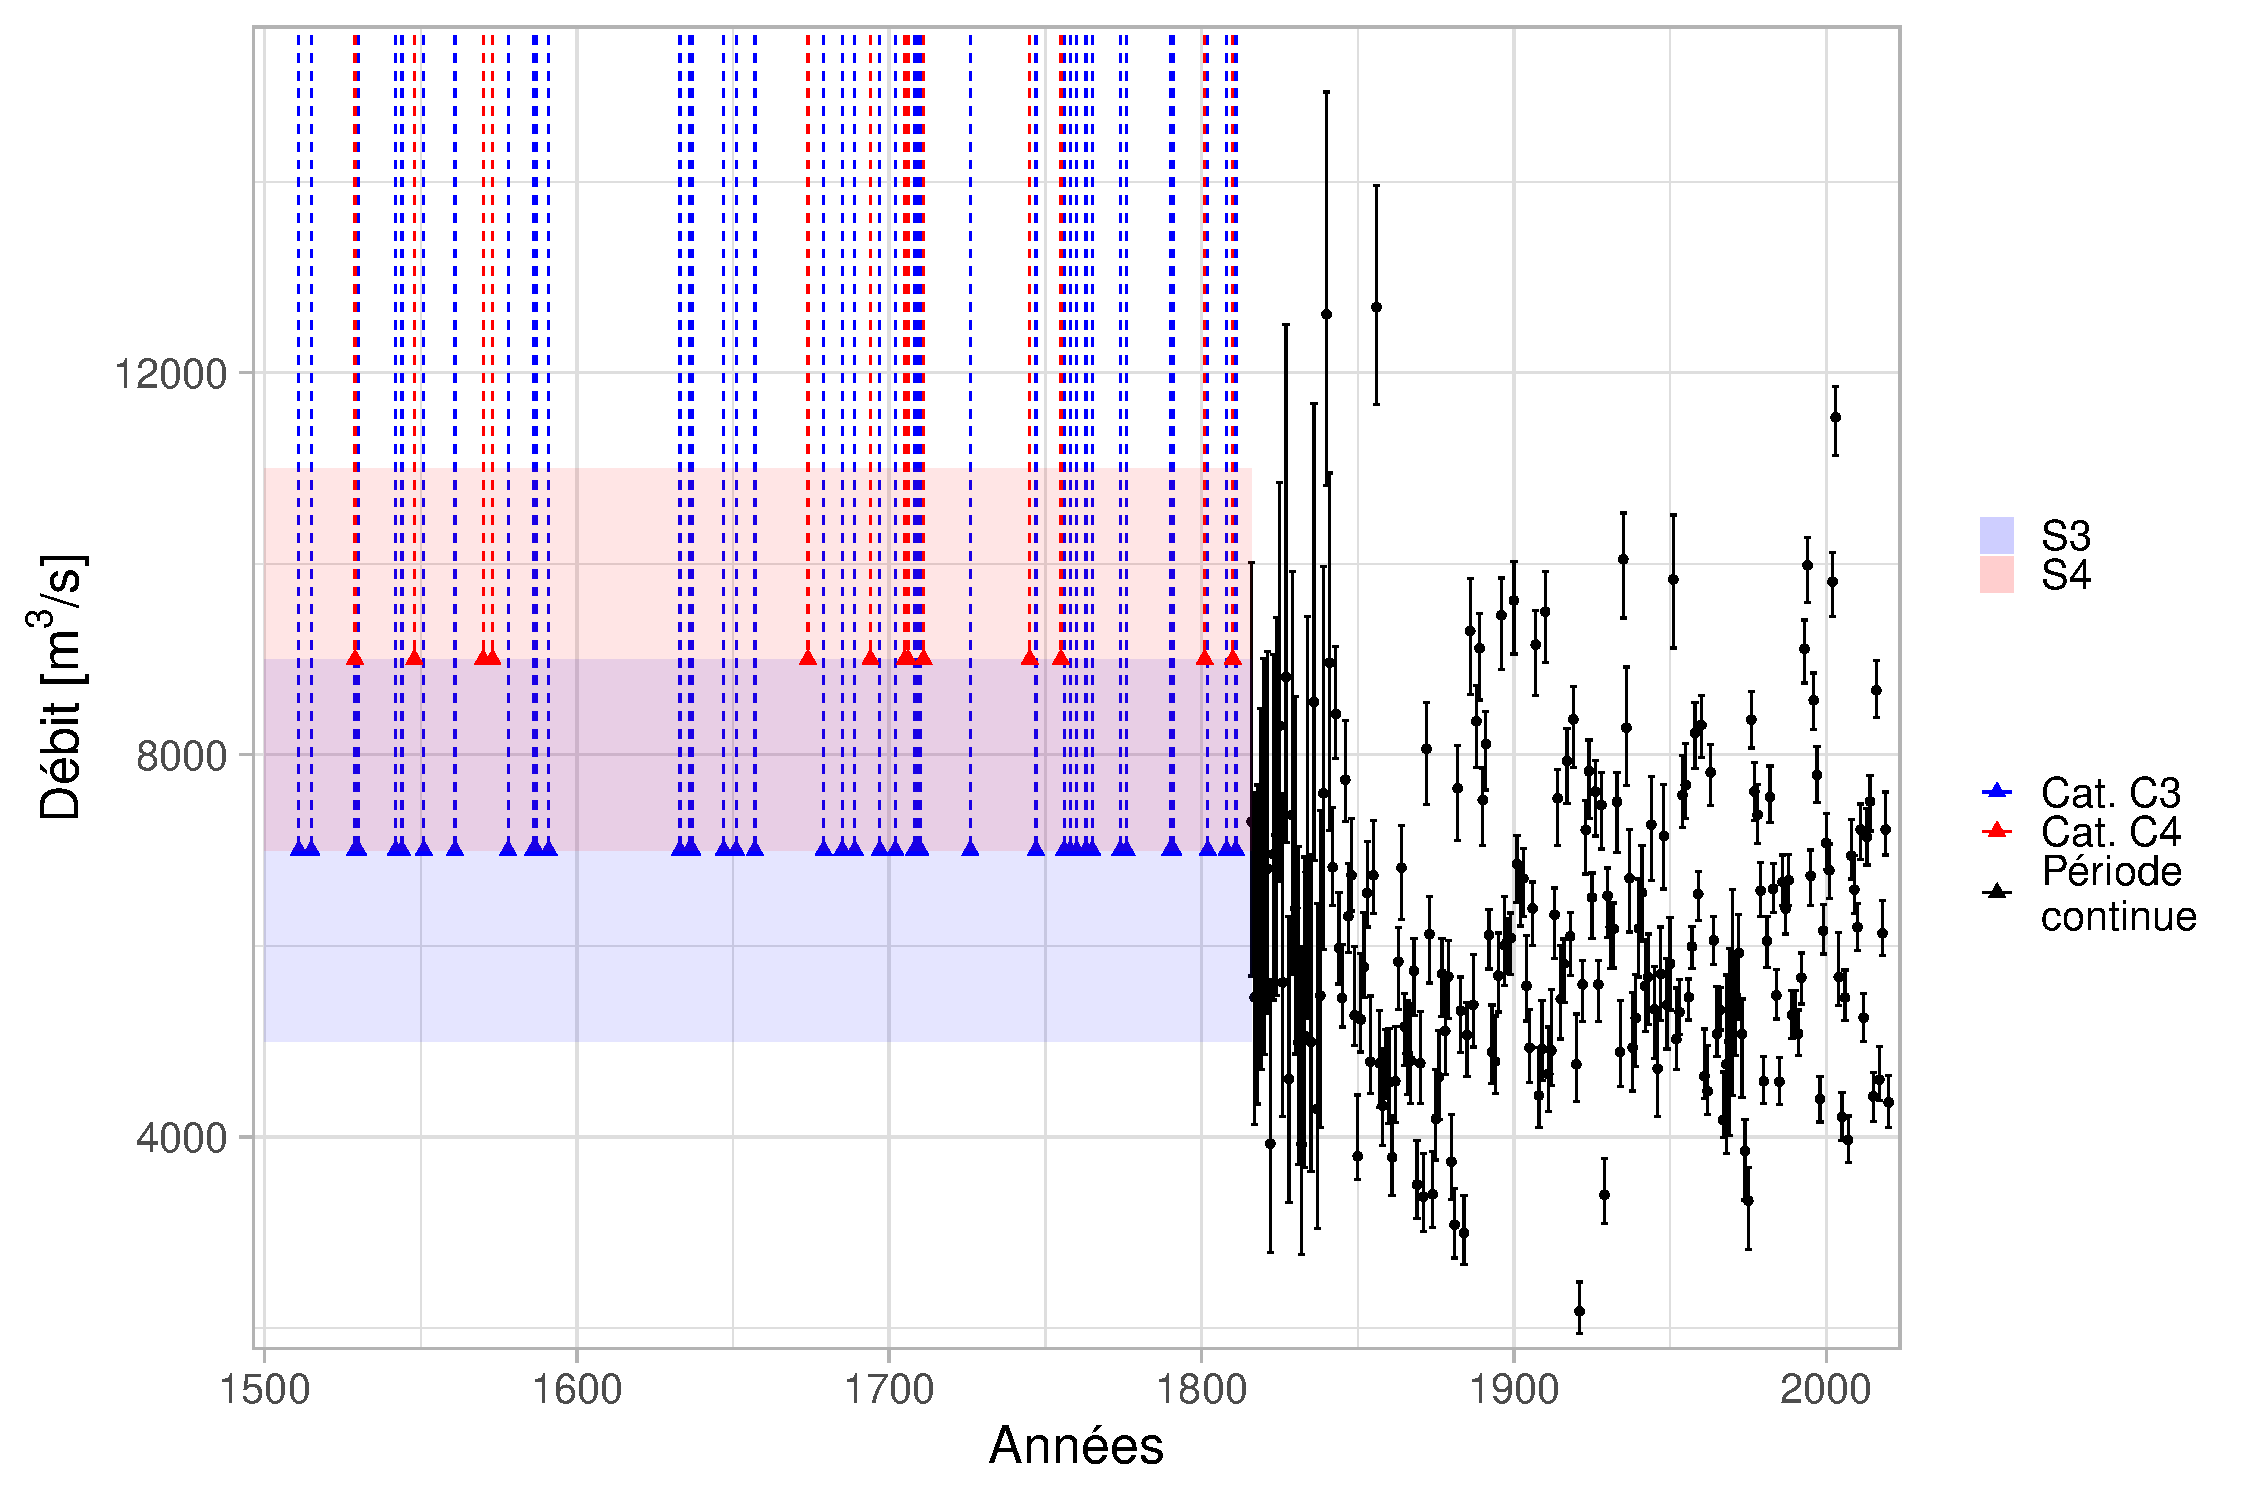
\includegraphics[width=.9\linewidth]{Chapitre4/Figures/EchMixteBcr.pdf}	
		\caption{Échantillon de crues du Rhône à Beaucaire. L'incertitude à 95\% autour des seuils de perception est représentée par les bandeaux bleu et rouge ("S3" et "S4)}
		\label{fig:EchMixte}
	\end{figure}
	

	\subsection{Homogénéité des données}
	\label{subsec:homog}
	\paragraph{} L'homogénéité des données est un pré-requis essentiel à l'analyse fréquentielle des crues en contexte stationnaire, car cette dernière repose sur l'hypothèse que les variables étudiées sont $iid$ (indépendantes et identiquement distribuées). C'est-à-dire que la distribution des crues ne change pas dans le temps et qu'une même distribution peut être utilisée pour modéliser les crues du XVI\textsuperscript{ème} et du XXI\textsuperscript{ème} siècle. Étant donné que deux types d'échantillons sont ici utilisés, deux types de tests statistiques sont appliqués dans les sections suivantes pour étudier l'homogénéité de ces données. 

	\subsubsection{Données continues}
	
	\paragraph{} Trois tests seront utilisés pour qualifier l'homogénéité de l'échantillon de données continues : le test de \citet{pettitt_non-parametric_1979} et la procédure de segmentation développée par \citet{darienzo_detection_2021-1} qui permettent de détecter des ruptures dans les séries temporelles, ainsi que le test de Mann-Kendall (\cite{mann_nonparametric_1945}; \cite{kendall_rank_1948}) qui permet de détecter l'existence de tendances. Les ruptures sont des changements soudains (i.e. les données ont une distribution différente avant et après un instant $t$, par exemple suite à un changement d'instrumentation), tandis que les tendances représentent des changements progressifs dans la distribution des données au cours du temps (par exemple : un changement progressif des conditions d'écoulement du bassin versant). Parmi ces trois tests, seule la procédure de segmentation de \citet{darienzo_detection_2021-1} permet de considérer l'incertitude des données d'entrée (déterminée au chapitre \ref{chap:ch3}).
	
	\paragraph{} La p-value des tests de Pettitt et Mann-Kendall appliqués à la série maxpost des débits maximum annuels à Beaucaire est respectivement de 0.15 et 0.41. Au risque d'erreur 5\%, on peut conclure qu'il n'existe pas de tendance ou de rupture dans la série. Il faut cependant s'assurer que ce résultat est toujours vrai lorsque l'on considère les incertitudes de la série.
			
	\paragraph{} L'application de la procédure de segmentation de \citet{darienzo_detection_2021-1} à la série de débits maximum annuels avec incertitude a conclu que le nombre optimal de segments pour la chronique de Beaucaire était de 1, et ce quel que soit le critère de segmentation considéré (AIC, BIC, HQC ou DIC). On peut ainsi conclure qu'aucune rupture n'existe dans les données. L'échantillon de données continues peut être considéré homogène suite aux tests statistiques réalisés. 
	
%	\paragraph{} Afin de d'étudier l'existence de tendances dans la série en considérant les incertitudes, le test de Mann-Kendall a été appliqué aux 500 réalisations possibles. Seulement 20\% des 500 p-values calculées sont inférieures à 0.05. Au risque d'erreur 5\%, on peut alors conclure que seulement 20\% des 500 réalisations de la série comportent une tendance. On peut calculer une valeur théorique ... A quelle valeur faudrait-il s'attendre pour considérer que c'est homogène (Benjamin ?) 

		
	\subsubsection{Données historiques}
	
	\paragraph{} Les données pré-enregistrements continus (ou historiques) utilisées ici prennent la forme d'occurrences de crues supposées supérieures à un seuil de perception. Comme décrit par \citet{lang_towards_1999}, la fréquence des occurrences de crues supérieures à un seuil est supposée suivre un processus de Poisson. Afin de vérifier l'homogénéité des occurrences de crues, il est possible de calculer un intervalle de confiance autour du nombre cumulé de crues découlant du processus de Poisson. Si les occurrences de crues cumulées "sortent" de cet intervalle de confiance, alors leur fréquence d'occurrence est supposée non-stationnaire. 
	
	\paragraph{} Ces intervalles de confiance ont été calculés pour l'échantillon de crues pré-enregistrements continus du Rhône à Beaucaire. La période historique est supposée débuter en 1500 et se termine à l'année des premiers enregistrements continus de hauteur d'eau, en 1816. Les deux échantillons testés ici reflètent deux seuils de perception, $S3$ et $S4$, et on a $S3 < S4$. 

	\begin{figure}[h]
		\centering
		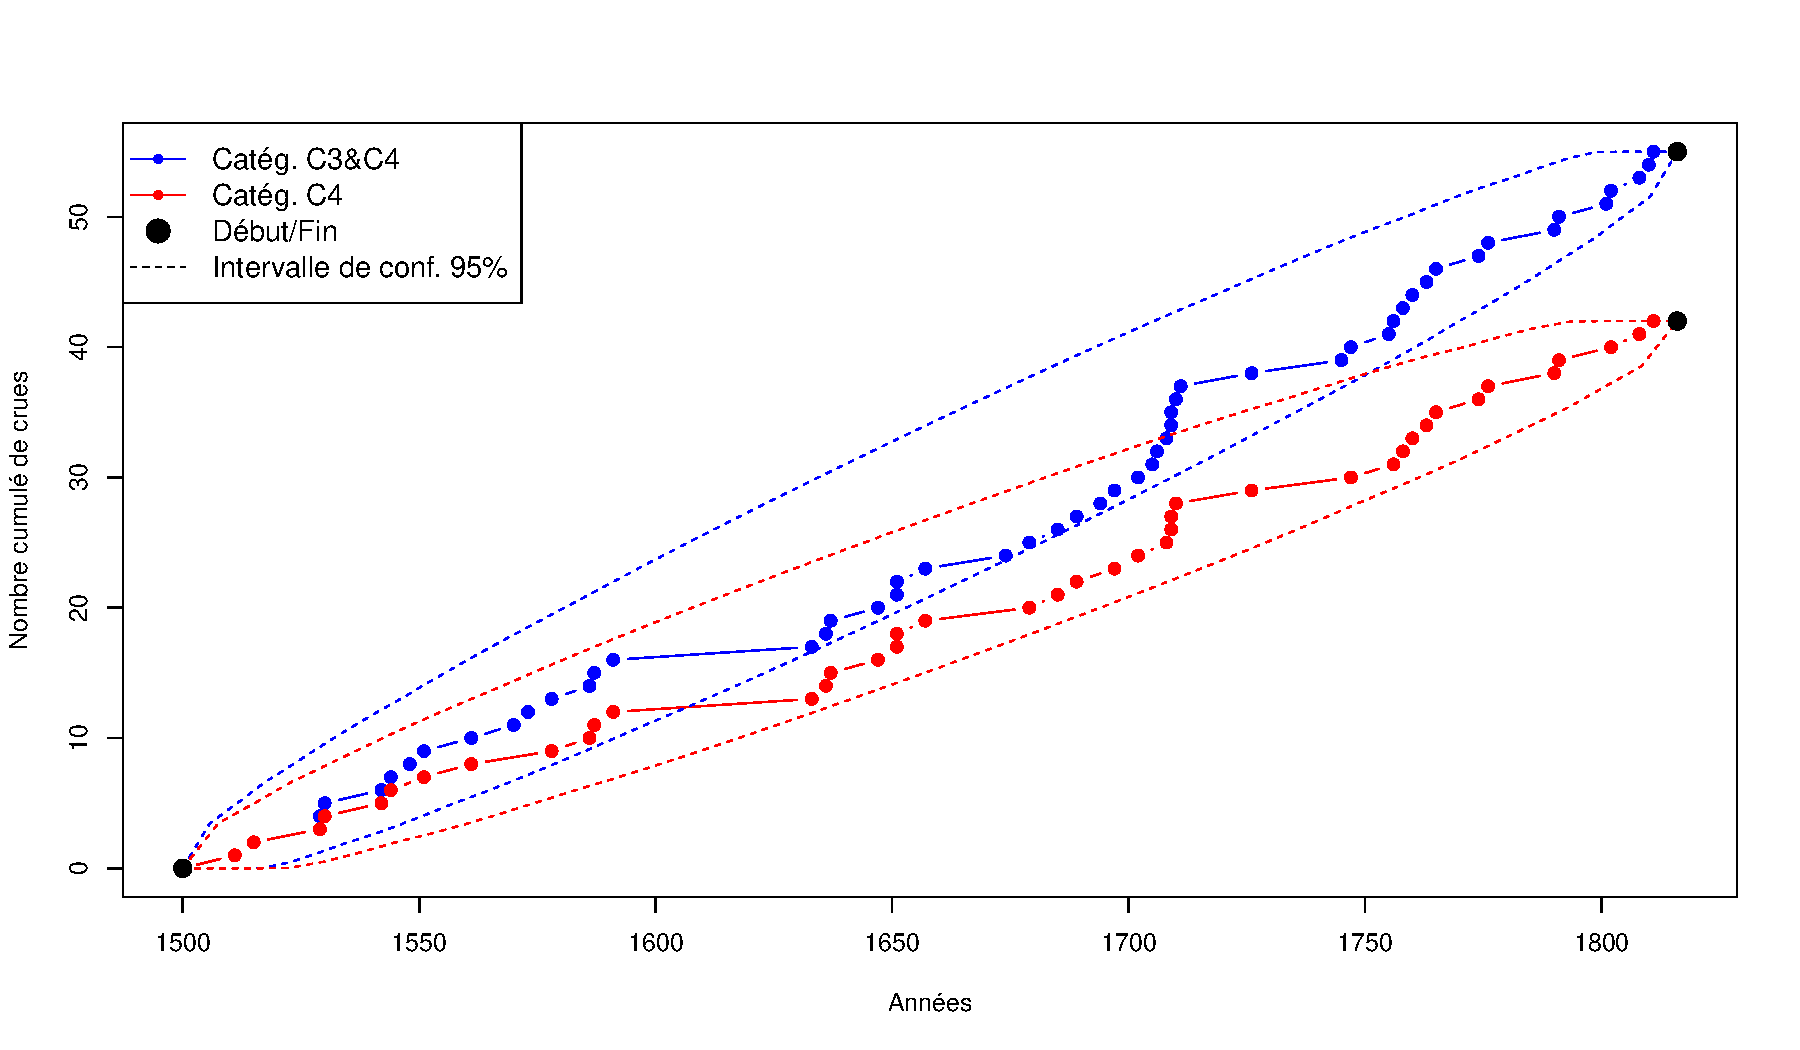
\includegraphics[width=.8\linewidth]{Chapitre4/Figures/Poisson_C3-C4_FR.pdf}	
		\caption{Nombre de crues cumulé et intervalles de confiance à 95\% du processus de 						Poisson, pour deux échantillons d'occurrences de crues supérieures aux seuils $S3$ (catégories C3 et C4) ou $S4$ (catégorie C4) à Beaucaire (1500-1816)}
		\label{fig:Poisson_C3-C4}
	\end{figure}		
	
	\paragraph{} Sur la figure \ref{fig:Poisson_C3-C4}, on remarque que les nombres cumulés de crues des deux échantillons sont compris dans les intervalles de confiance à 95\% des processus de Poisson, ils peuvent donc être tous deux considérés homogènes. L'échantillon correspondant au seuil $S3$ (en bleu) se rapproche de la borne inférieure de l'intervalle de confiance au XVII\textsuperscript{ème} siècle, mais revient rapidement dans des valeurs moyennes à la faveur de nombreuses crues supérieures au seuil au début du XVIII\textsuperscript{ème} siècle. 
	
	\paragraph{} L'échantillon continu de débits maximum annuels (1816-2020) sera par la suite artificiellement "dégradé" pour reproduire des durées de chroniques plus usuelles. Ainsi, les crues dont le débit maxpost est supérieur au seuil considéré sont retenues dans l'échantillon. Cette période "dégradée" commence au début de la chronique, en 1816, et se termine en 1970, à la mise en fonctionnement de la station de Beaucaire Restitution. Deux seuils de perception similaires aux seuils $S3$ et $S4$ sont ici étudiés : 7000 et 9000 $m^3/s$. L'homogénéité de ces deux échantillons "dégradés" est testée dans la figure \ref{fig:Poisson_Recent}. Les deux échantillons de crues cumulés sont compris dans les intervalles de confiance à 95\%, ils sont donc tous deux homogènes. 
	
	\begin{figure}[h]
		\centering
		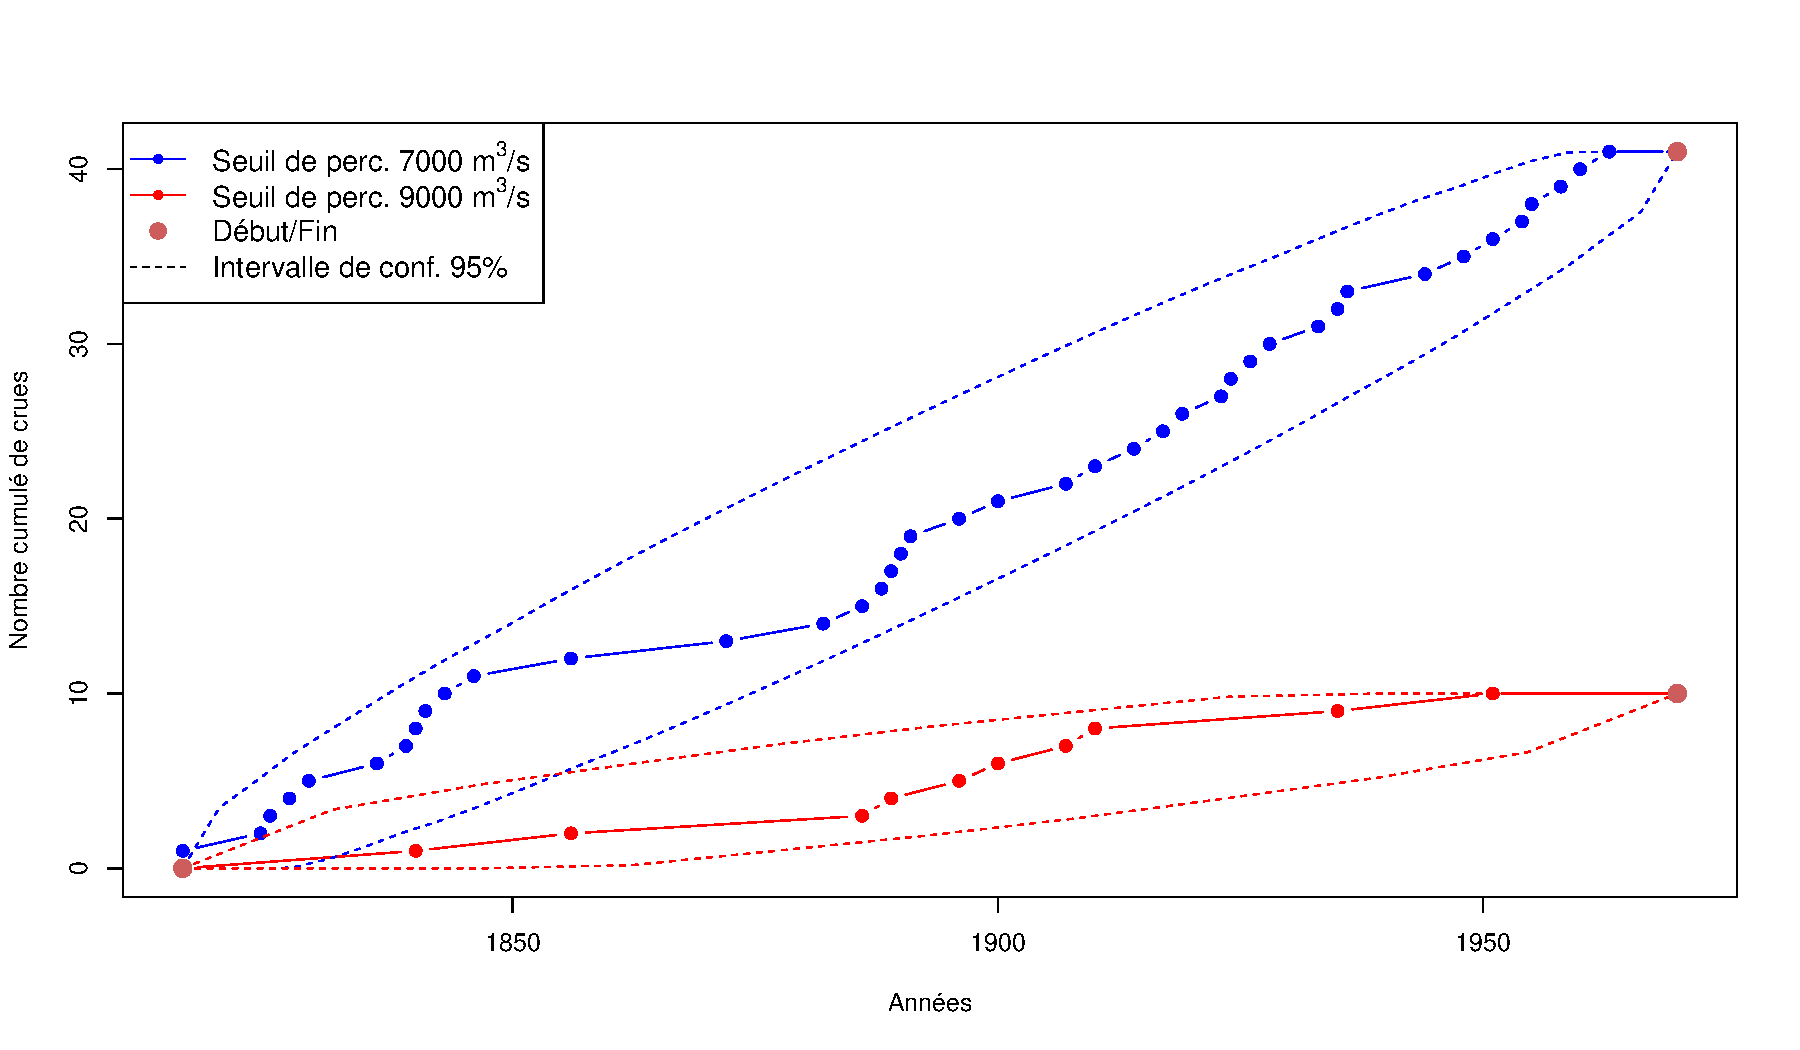
\includegraphics[width=.8\linewidth]{Chapitre4/Figures/Poisson_Qrecent_FR.pdf}	
		\caption{Nombre de crues cumulé et intervalles de confiance à 95\% du processus de 						Poisson, pour deux échantillons d'occurrences de crues supérieures aux seuils $S3$ ou $S4$ à Pont de Beaucaire 							(1816-1969) }
		\label{fig:Poisson_Recent}
	\end{figure}
	
	
	\paragraph{} Les échantillons de crues des périodes systématique et historique ont indépendamment été jugés homogènes. Il faut cependant garder à l'esprit que ces échantillons peuvent ne pas être homogènes entre eux pour diverses raisons. Par exemple, le seuil de perception utilisé pour l'échantillon systématique ($S3$ ou $S4$) peut ne pas être cohérent avec le seuil de perception de l'échantillon historique dont la valeur exacte est inconnue. 		
		
\FloatBarrier		
	
	
\section{Application aux crues du Rhône à Beaucaire}
\label{sec:applicationBcr}

	\paragraph{} Les 4 modèles décrits dans les sections précédentes (A, B, C et D) sont appliqués aux 4 échantillons de crues du Rhône à Beaucaire présentés dans le tableau \ref{tab:Echantillons}. Le modèle A fait l'hypothèse que le seuil de perception $S$ et la durée de la période historique $n$ sont parfaitement connus, tandis que dans le cas du modèle D, ces deux valeurs sont considérées incertaines. Le modèle B fait l'hypothèse que seul le seuil de perception $S$ est incertain, alors que pour le modèle C, seule la durée de la période historique $n$ est incertaine. Le modèle E suppose quant a lui que le débit des crues historique est connu et est contenu dans un intervalle d'incertitude, $S$ et $n$ sont alors supposés parfaitement connus. Pour les cinq modèles, l'incertitude des débits de la période continue est propagée. 
	
	\paragraph{} Les échantillons 1 et 2 représentent la combinaison des données pré-1816 décrites dans le chapitre \ref{chap:ch2} avec les données continues 1816-2020 estimées au chapitre \ref{chap:ch3}. Les échantillons 3 et 4 sont basés sur les débits estimés au chapitre \ref{chap:ch3} qui ont été dégradés pour créer artificiellement un échantillon mixte de données continues (1970-2020) et ponctuelles (1816-1969). Il s'agit ici de tailles d'échantillon plus usuelles et dont le seuil de perception et la durée de la période historique sont parfaitement connus, contrairement aux échantillons 1 et 2. Ainsi, pour les modèles faisant l'hypothèse que le seuil de perception et/ou la durée de la période historique sont inconnus, on jugera notamment la capacité du modèle à estimer des valeurs acceptables. 
	
	\begin{table}[h]
		\centering
		\caption{Caractéristiques des échantillons de crues du Rhône à Beaucaire. $S$ désigne le seuil de perception et $t^{*}$ la date de début de la période historique.}
		\label{tab:Echantillons}
		\resizebox{\columnwidth}{!}{%
		%\begin{tabular}{|l|l|l|l|ll|l|l|}
		\begin{tabular}{|c|c|c|c|cc|c|c|}
		\hline
		\multicolumn{1}{|c|}{\multirow{2}{*}{n°}} &
		  \multirow{2}{*}{Période historique} &
		  \multirow{2}{*}{Période continue} &
		  \multirow{2}{*}{Seuil $S$ [m\textsuperscript{3}/s]} &
		  \multicolumn{2}{c|}{Nb. de crues $> S$} &
		  \multirow{2}{*}{A priori $S$ [m\textsuperscript{3}/s]} &
		  \multirow{2}{*}{A priori $t^{*}$} \\ \cline{5-6}
		  
		 \multicolumn{1}{|c|}{} & & & & \multicolumn{1}{c|}{per. hist.} & per. cont. & & \\ \hline
		1 & 1500-1815 & 1816-2020 & 7000 & \multicolumn{1}{c|}{55} & 57 & $\mathcal{N}(7000,2000)$ & $\mathcal{U}(1111,1511)$ \\ \hline
		2 & 1500-1815 & 1816-2020 & 9000 & \multicolumn{1}{c|}{13} & 14 & $\mathcal{N}(9000,2000)$ & $\mathcal{U}(1129,1529)$ \\ \hline
		3 & 1816-1969 & 1970-2020 & 7000 & \multicolumn{1}{c|}{41} & 16 & $\mathcal{N}(7000,2000)$ & $\mathcal{U}(1316,1816)$ \\ \hline
		4 & 1816-1969 & 1970-2020 & 9000 & \multicolumn{1}{c|}{10} & 4 & $\mathcal{N}(9000,2000)$ & $\mathcal{U}(1340,1840)$ \\ \hline
		\end{tabular}%
		}
		
	\end{table}		
	
	Les modèles B, C et D font l'hypothèse que $S$ et/ou $n$ sont inconnus, il faudra donc affecter une distribution a priori à ces paramètres. Ces distributions sont présentées dans le tableau \ref{tab:Echantillons} pour chacun des échantillons. Le but étant ici d'explorer les performances des modèles, les a priori seront très peu informatifs. L'a priori du seuil de perception $S$ (modèles B et D) est supposé Gaussien, avec pour moyenne la valeur connue ou supposée du seuil (soit $S3$ ou $S4$) et pour écart type 2000 m\textsuperscript{3}/s. Par souci de clarté, on ne parlera pas ici de la durée de la période historique $n$ mais de la date de début de la période historique $t^{*}$ (la date de fin de la période historique étant ici parfaitement connue pour les 4 échantillons). La distribution a priori de $t^{*}$ (modèles C et D) est supposée uniforme avec pour borne supérieure la date de la première crue de l'échantillon historique considéré, appelée $t_{k=1}$. Par définition, la période historique débute au plus tard à la date de cette première crue. La borne inférieure de la distribution uniforme sera fixée 400 ans avant la date de la première crue $t_{k=1}$ afin de représenter la méconnaissance de $t^{*}$. 
			
	\FloatBarrier	
	
	\subsection{Résultats pour la période récente dégradée (1816-2020)}
	\label{subsec:ResultsArtif}
	
	\paragraph{} 
	Les 4 modèles décrits dans la section \ref{sec:MethodoCh3} ont été appliqués à l'échantillon 4 du tableau \ref{tab:Echantillons}. Les estimations pour les crues centennales et millénales sont présentées dans la figure \ref{fig:Barplot_Artif2}, dans laquelle les 4 modèles GEV-Binomiale sont comparés au modèle GEV (chapitre \ref{chap:ch3}) appliqué successivement à la chronique continue totale (1816-2020) et à la chronique continue dégradée (1970-2020). Ces mêmes résultats sont détaillés dans le tableau \ref{tab:ResArtif2}, où la valeur des paramètres est présentée. Enfin, la figure \ref{fig:Quantiles_Artif2} présente l'ensemble des quantiles jusqu'à la crue décamillénale pour les 6 modèles. On peut ici juger l'adéquation des quantiles avec les observations. Le rang des crues supérieures au seuil est tiré aléatoirement comme décrit dans la section \ref{subsec:DistEmpirique}. 	
	
	\begin{figure}[h]
		\centering
		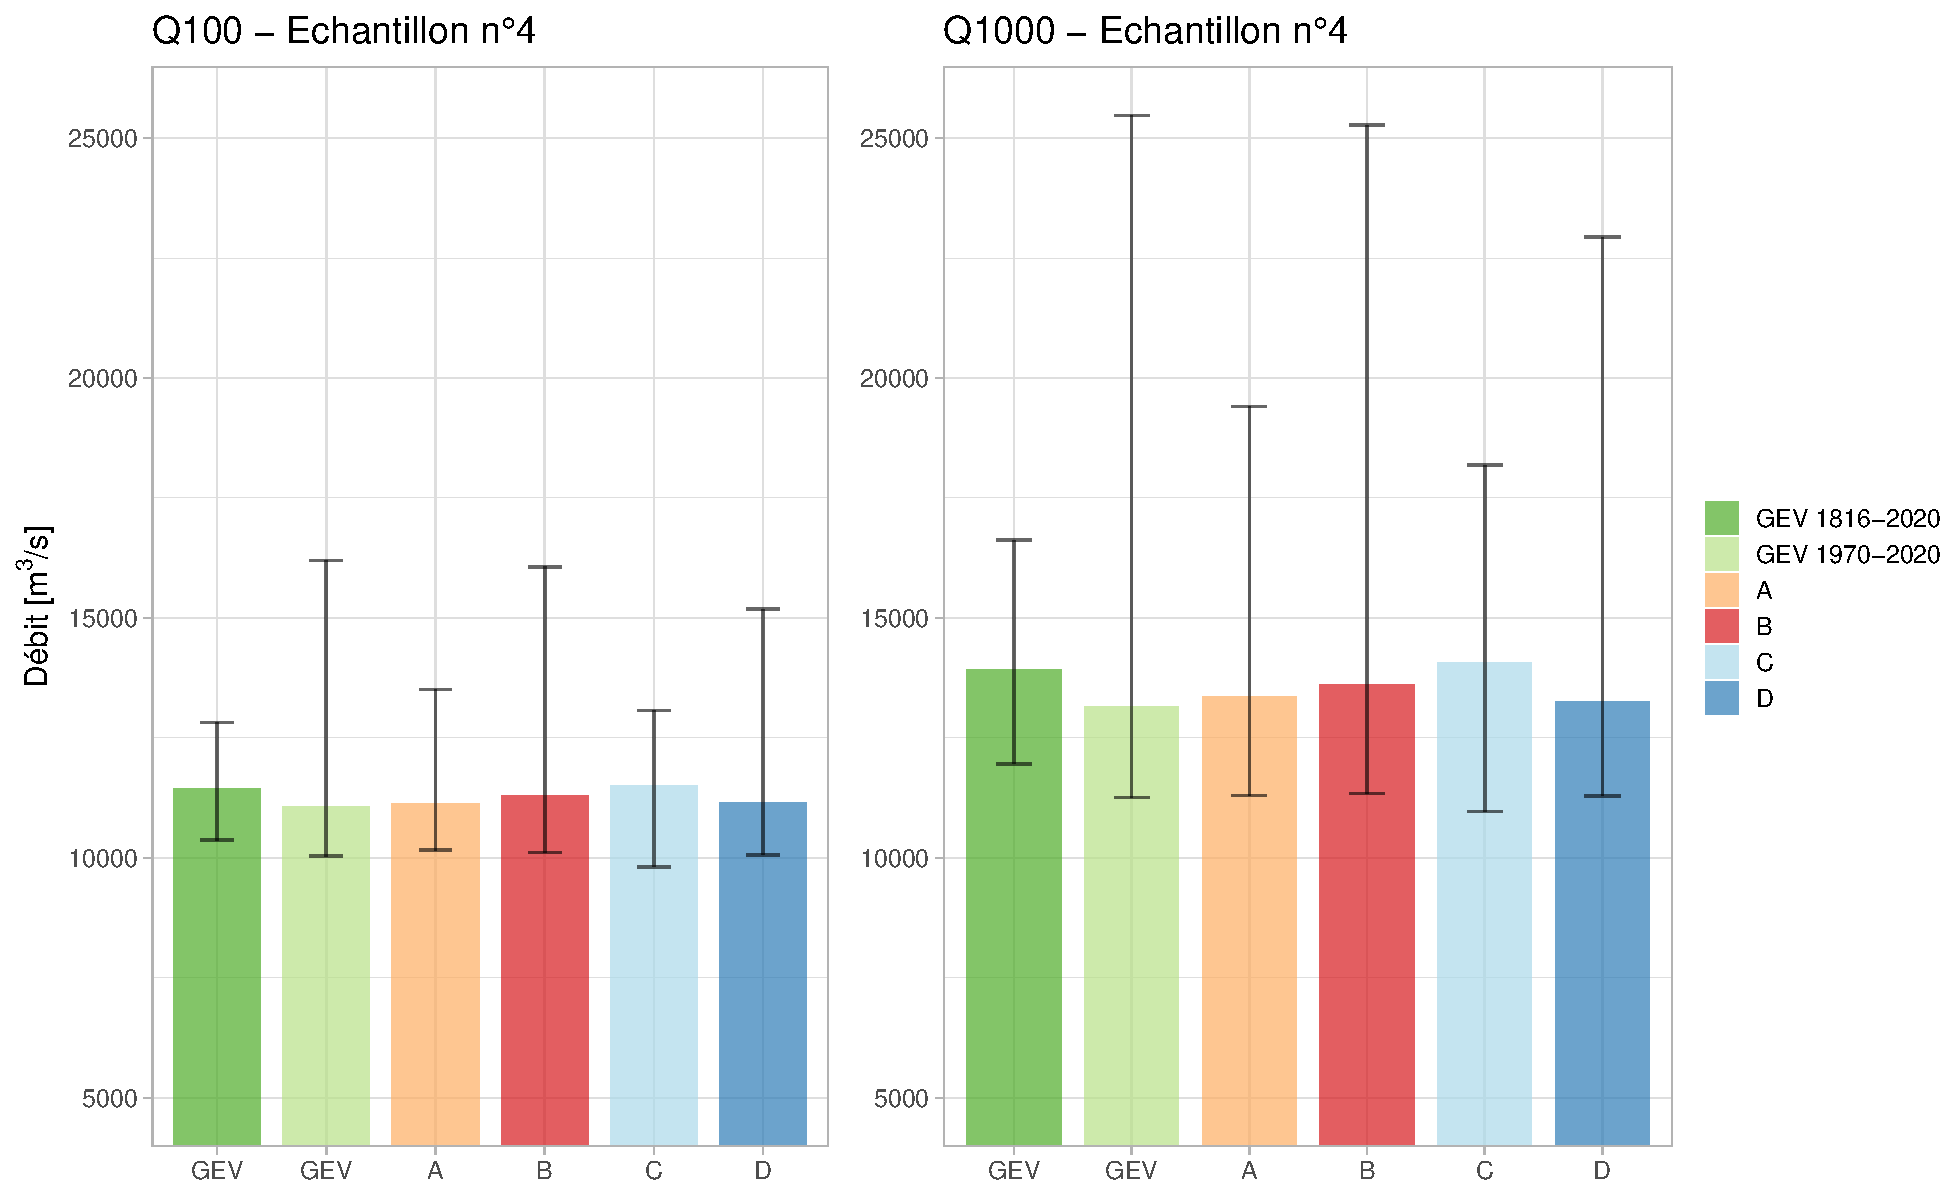
\includegraphics[width=.8\linewidth]{Chapitre4/Figures/Barplots_QX_Artif2.pdf}	
		\caption{Estimations maxpost et incertitudes à 95\% pour Q100 et Q1000 pour 6 modèles appliqués à l'échantillon 4 (1816-2020 dégradé, $S4$)}
		\label{fig:Barplot_Artif2}
	\end{figure}

	\begin{table}[h]
	\centering
	\caption{Résultats maxpost et incertitudes des 7 modèles appliqués à l'échantillon 4. Q100 et Q1000 représentent respectivement le débit des crues centennales et millénales, $\xi$ le paramètre de forme de la distribution GEV, $S$ le seuil de perception et $t^{*}$ la date de début de la période historique. Les écarts type des distributions a posteriori sont représentés par les colonnes débutant par la lettre "u". \textcolor{red}{DEPLACER PLUS PROCHE DE LA PARTIE MODELE E?} }
	\label{tab:ResArtif2}
	\resizebox{\columnwidth}{!}{%
		\begin{tabular}{|c|c|c|c|c|c|c|c|c|c|c|}
		\hline
Modèle & Q100 [m\textsuperscript{3}/s] & uQ100 [m\textsuperscript{3}/s] & Q1000 [m\textsuperscript{3}/s] & uQ1000 [m\textsuperscript{3}/s] & $\xi$ & $u\xi$ & $S$ [m\textsuperscript{3}/s] & $uS$ [m\textsuperscript{3}/s] & $t^{*}$ & $ut^{*}$ \\ \hline
GEV 1816-2020 & 11451 & 687   & 13919 & 1351   & 0.058 & 0.044  & X    & X    & X    & X  \\ \hline
GEV 1970-2020 & 11076 & 2560  & 13154 & 6159   & 0.077 & 0.102  & X    & X    & X    & X  \\ \hline
A             & 11132 & 1189  & 13367 & 3019   & 0.062 & 0.088  & 9000 & X    & 1816 & X  \\ \hline
B             & 11302 & 2381  & 13622 & 5823   & 0.058 & 0.102  & 9163 & 729  & 1816 & X  \\ \hline
C             & 11517 & 779   & 14069 & 2057   & 0.041 & 0.083  & 9000 & X    & 1833 & 71 \\ \hline
D             & 11147 & 2018  & 13262 & 4837   & 0.074 & 0.096  & 9332 & 883  & 1785 & 107 \\ \hline
E       	  & 11286 & 932   & 13827 & 2255   & 0.039 & \textcolor{red}{??} &  9000 & X & 1816 & X \\ \hline
		\end{tabular}}

	\end{table}

	\begin{figure}[h]
		\centering
		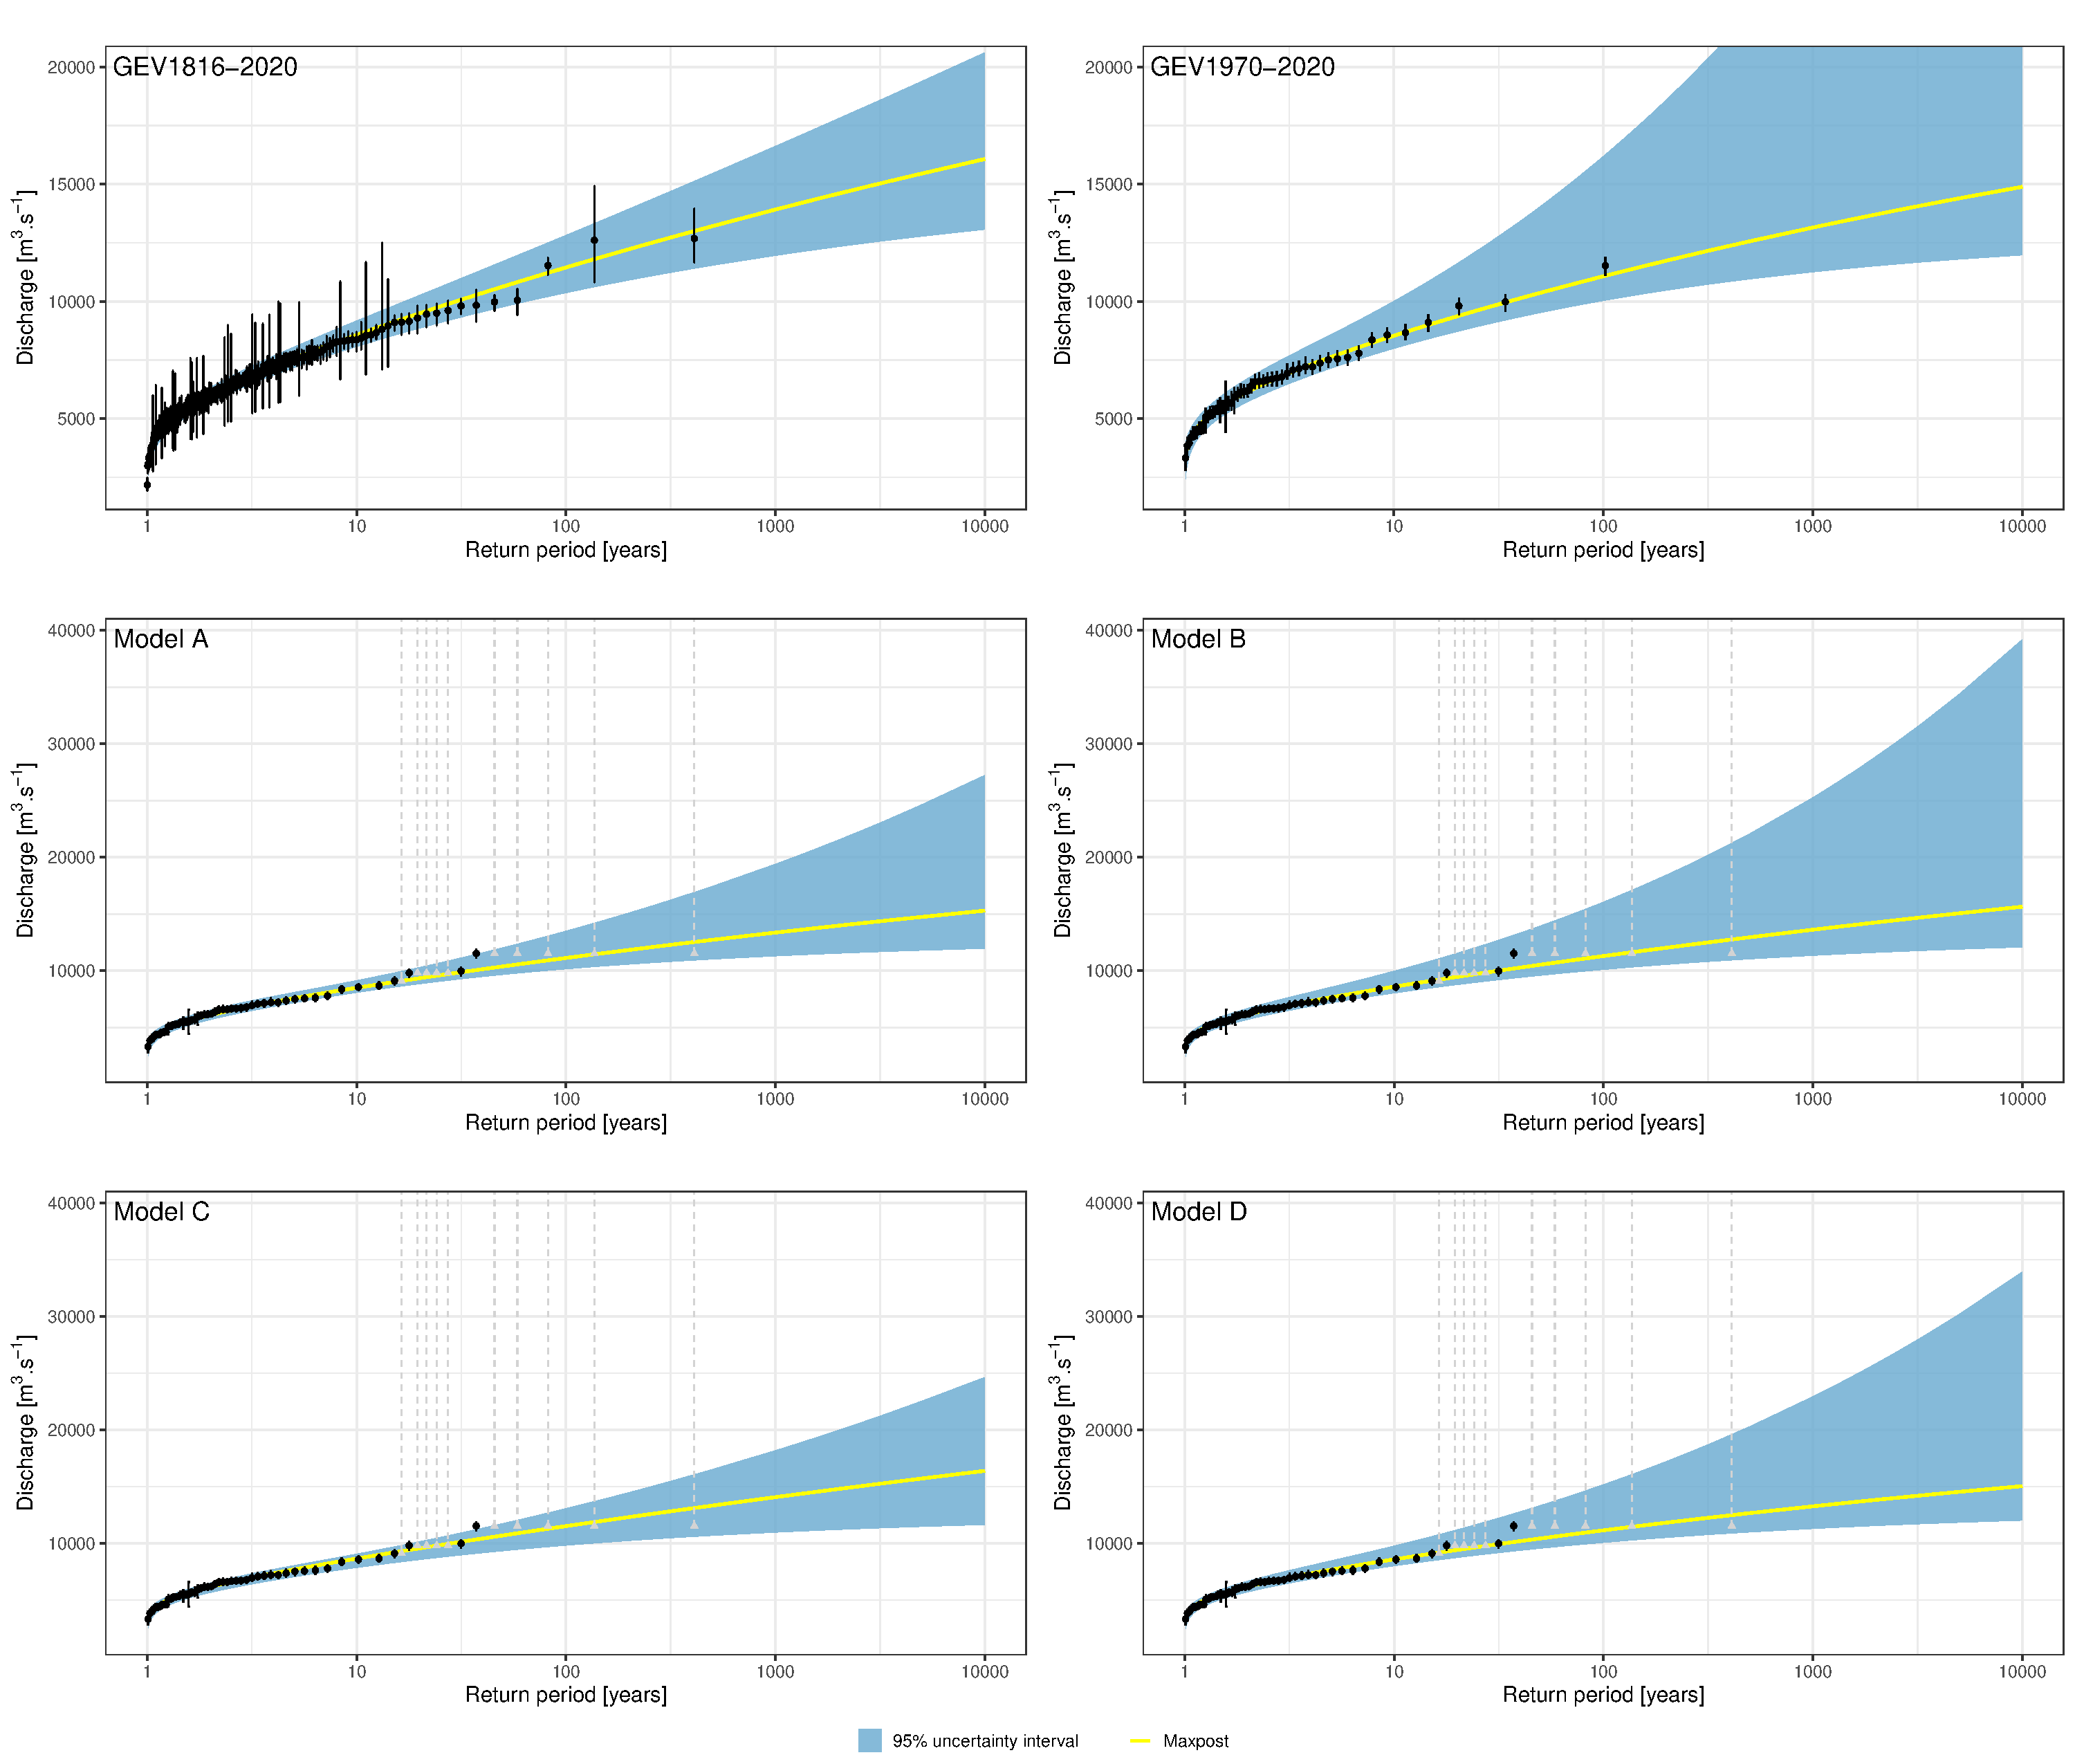
\includegraphics[width=\linewidth]{Chapitre4/Figures/Quantiles_Artif2.pdf}	
		\caption{Quantiles de débit maximum annuel estimés par 6 modèles pour l'échantillon 4 (1816-2020 dégradé, $S4$). Les observations sont en noir pour la période continue (l'incertitude est également représentée) et en gris pour la période historique.}
		\label{fig:Quantiles_Artif2}
	\end{figure}
	

\FloatBarrier
	
	\subsubsection{Quel est l'apport de l'utilisation des crues historiques pour une longueur de chronique "courante" ?}
	
	\paragraph{} Une durée de chronique continue trop courte devant la période de retour du quantile visé entraîne des résultats très incertains (GEV 1970-2020 dans les figures \ref{fig:Barplot_Artif2} et \ref{fig:Quantiles_Artif2}). La durée de la chronique continue (50 ans) est ici très petite devant la période de retour visée (100 ou 1000 ans). Si on se trouve dans l'impossibilité de reconstituer des débits en continu au-delà de 50 ans, on remarque que l'utilisation d'occurrences de crues historiques permet de réduire l'incertitude (modèle A en orange). Évidemment, l'utilisation d'occurrences de crues ne permet pas d'atteindre la précision obtenue avec 200 ans de chronique continue (GEV 1816-2020 en vert foncé), mais l'incertitude obtenue s'en rapproche en utilisant les crues historiques, tout particulièrement lorsque $S$ et $n$ sont connus. En revanche, les estimations maxpost de l'ensemble des modèles sont proches. 
	
	\paragraph{} Pour les 6 modèles, une part de l'incertitude provient de l'estimation du paramètre de forme qui gouverne le comportement de la queue de distribution. On retrouve les valeurs a posteriori du paramètre de forme dans la figure \ref{fig:Shape_Artif2}. On notera que l'ensemble des estimations sont proches de zéro et légèrement positives, on se trouve donc dans le cas "queue légère" de la distribution GEV (cas "loi de Weibull"). Comme l'on peut s'y attendre, l'estimation de ce paramètre est plus précise dans le cas GEV 1816-2020. Les distributions a posteriori sont très proches pour les modèles A et C (tableau \ref{tab:ResArtif2}). 
	
	\textcolor{red}{
	\paragraph{RMQ BEN} D'ailleurs comme on ne réduit que faiblement l'incertitude sur xi par rapport à GEV 1970-2020, d'où vient la réduction d'incertitude des quantiles? De position et échelle j'imagine? Comme tu as de la place en figure 6 est-ce que ca ne vaudrait pas le coup de mettre les 3 paramètres? A FAIRE S'IL RESTE DU TEMPS
	}
	
	\begin{figure}[h]
		\centering
		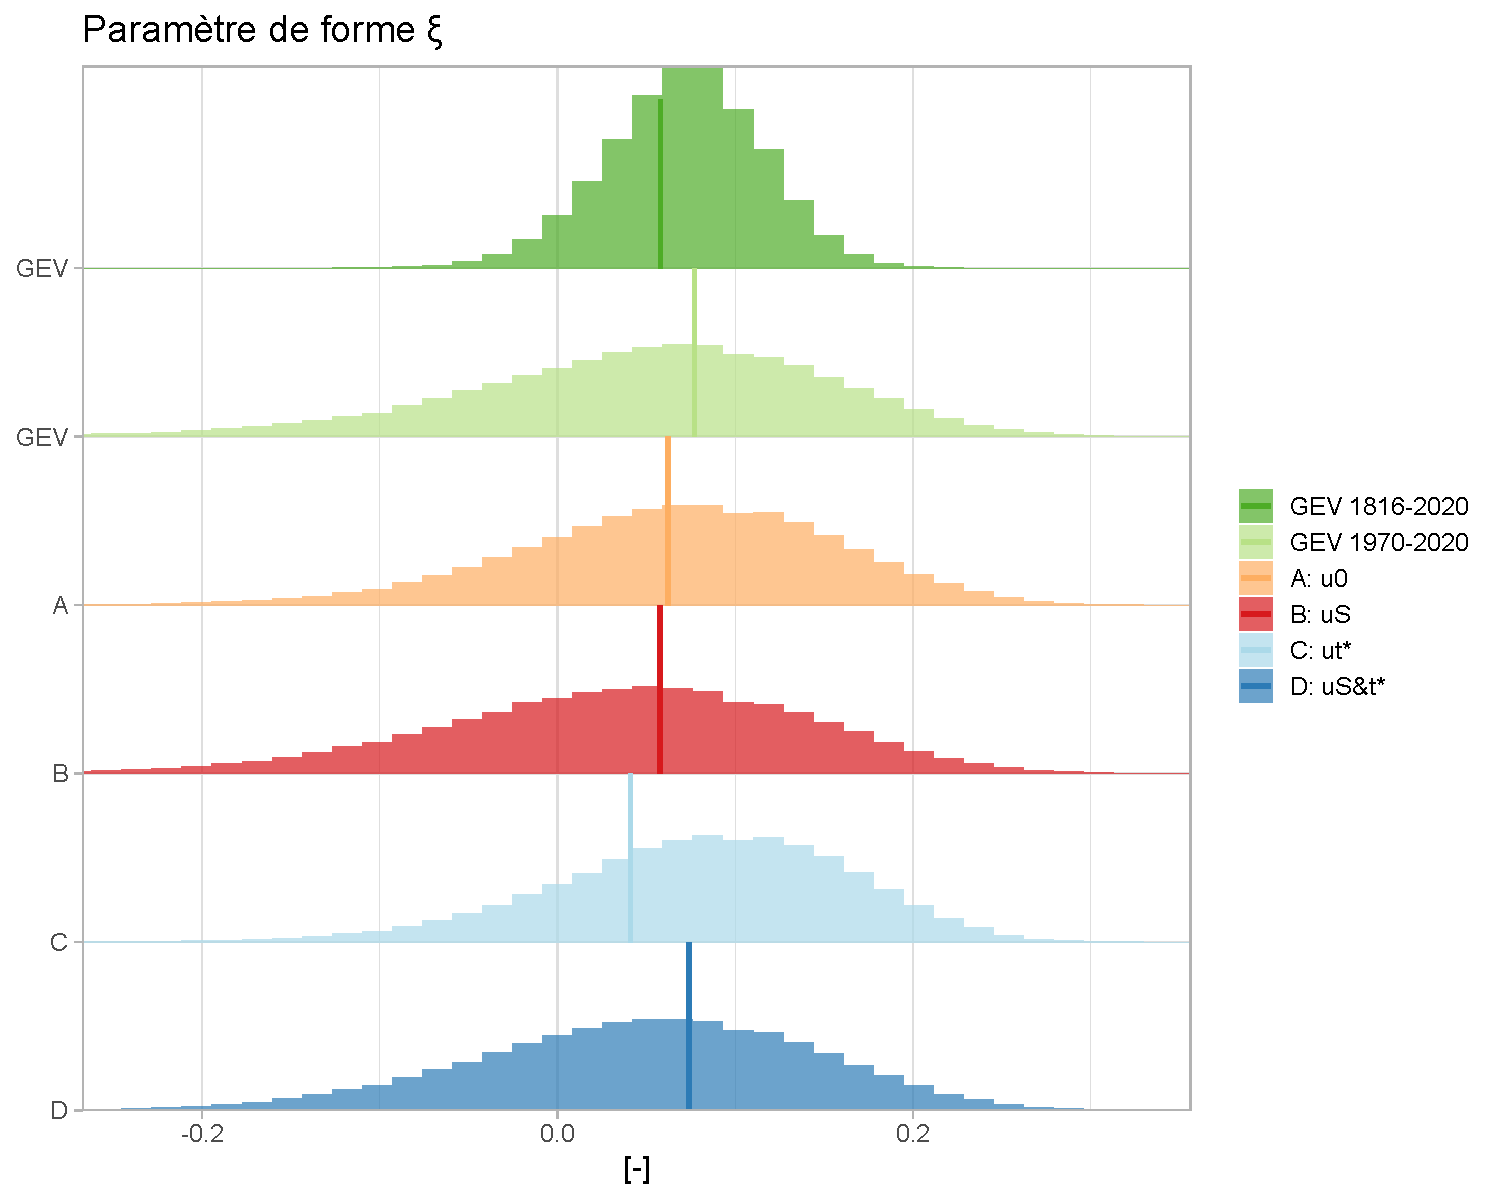
\includegraphics[width=.6\linewidth]{Chapitre4/Figures/Shape_Artif2.pdf}	
		\caption{Distributions a posteriori du paramètre de forme de la distribution GEV des débits maximum annuels pour les 4 modèles estimés sur l'échantillon 4. Les estimations des modèles GEV sont également indiquées. Les droites verticales représentent les valeurs maxpost.}
		\label{fig:Shape_Artif2}
	\end{figure}

\FloatBarrier
	
	\subsubsection{Quel est l'impact de la méconnaissance du seuil de perception sur l'estimation des quantiles ?}
	
	\paragraph{} L'utilisation du modèle B reflète la méconnaissance du seuil de perception, celui-ci devenant alors un paramètre à part entière du modèle. Sur la figure \ref{fig:Barplot_Artif2}, on constate que l'incertitude autour des quantiles estimés par le modèle B est bien plus importante que pour le modèle A, et se rapproche de celle obtenue avec les données continues seulement (GEV 1970-2020). La méconnaissance du seuil a donc des conséquences importantes sur les estimations puisqu'elle réduit fortement l'intérêt d'utiliser les occurrences historiques. La vraie valeur du seuil de perception pour l'échantillon 4 est $S4$ = 9000 m\textsuperscript{3}/s. On retrouve les distributions a priori et a posteriori du seuil dans la figure \ref{fig:Params_Artif2}. On remarque que l'a posteriori pour le modèle B est proche de la vraie valeur, et que le modèle a effectivement permis d'améliorer la connaissance du seuil par rapport à l'a priori renseigné qui est ici très incertain : $\mathcal{N}(9000,2000)$. La valeur maxpost est de 9163 m\textsuperscript{3}/s soit une erreur relative de 2\%. Dans une situation plus réaliste, un a priori du seuil de perception plus précis aurait pu être choisi afin de limiter cet impact. Il faut également noter que l'incertitude a posteriori du paramètre de forme pour le modèle B (figure \ref{fig:Shape_Artif2}) est plus grande que celle du modèle A et devient alors quasi-identique à celle du modèle GEV 1970-2020. 
	
	 \begin{figure}[h]
		\centering
		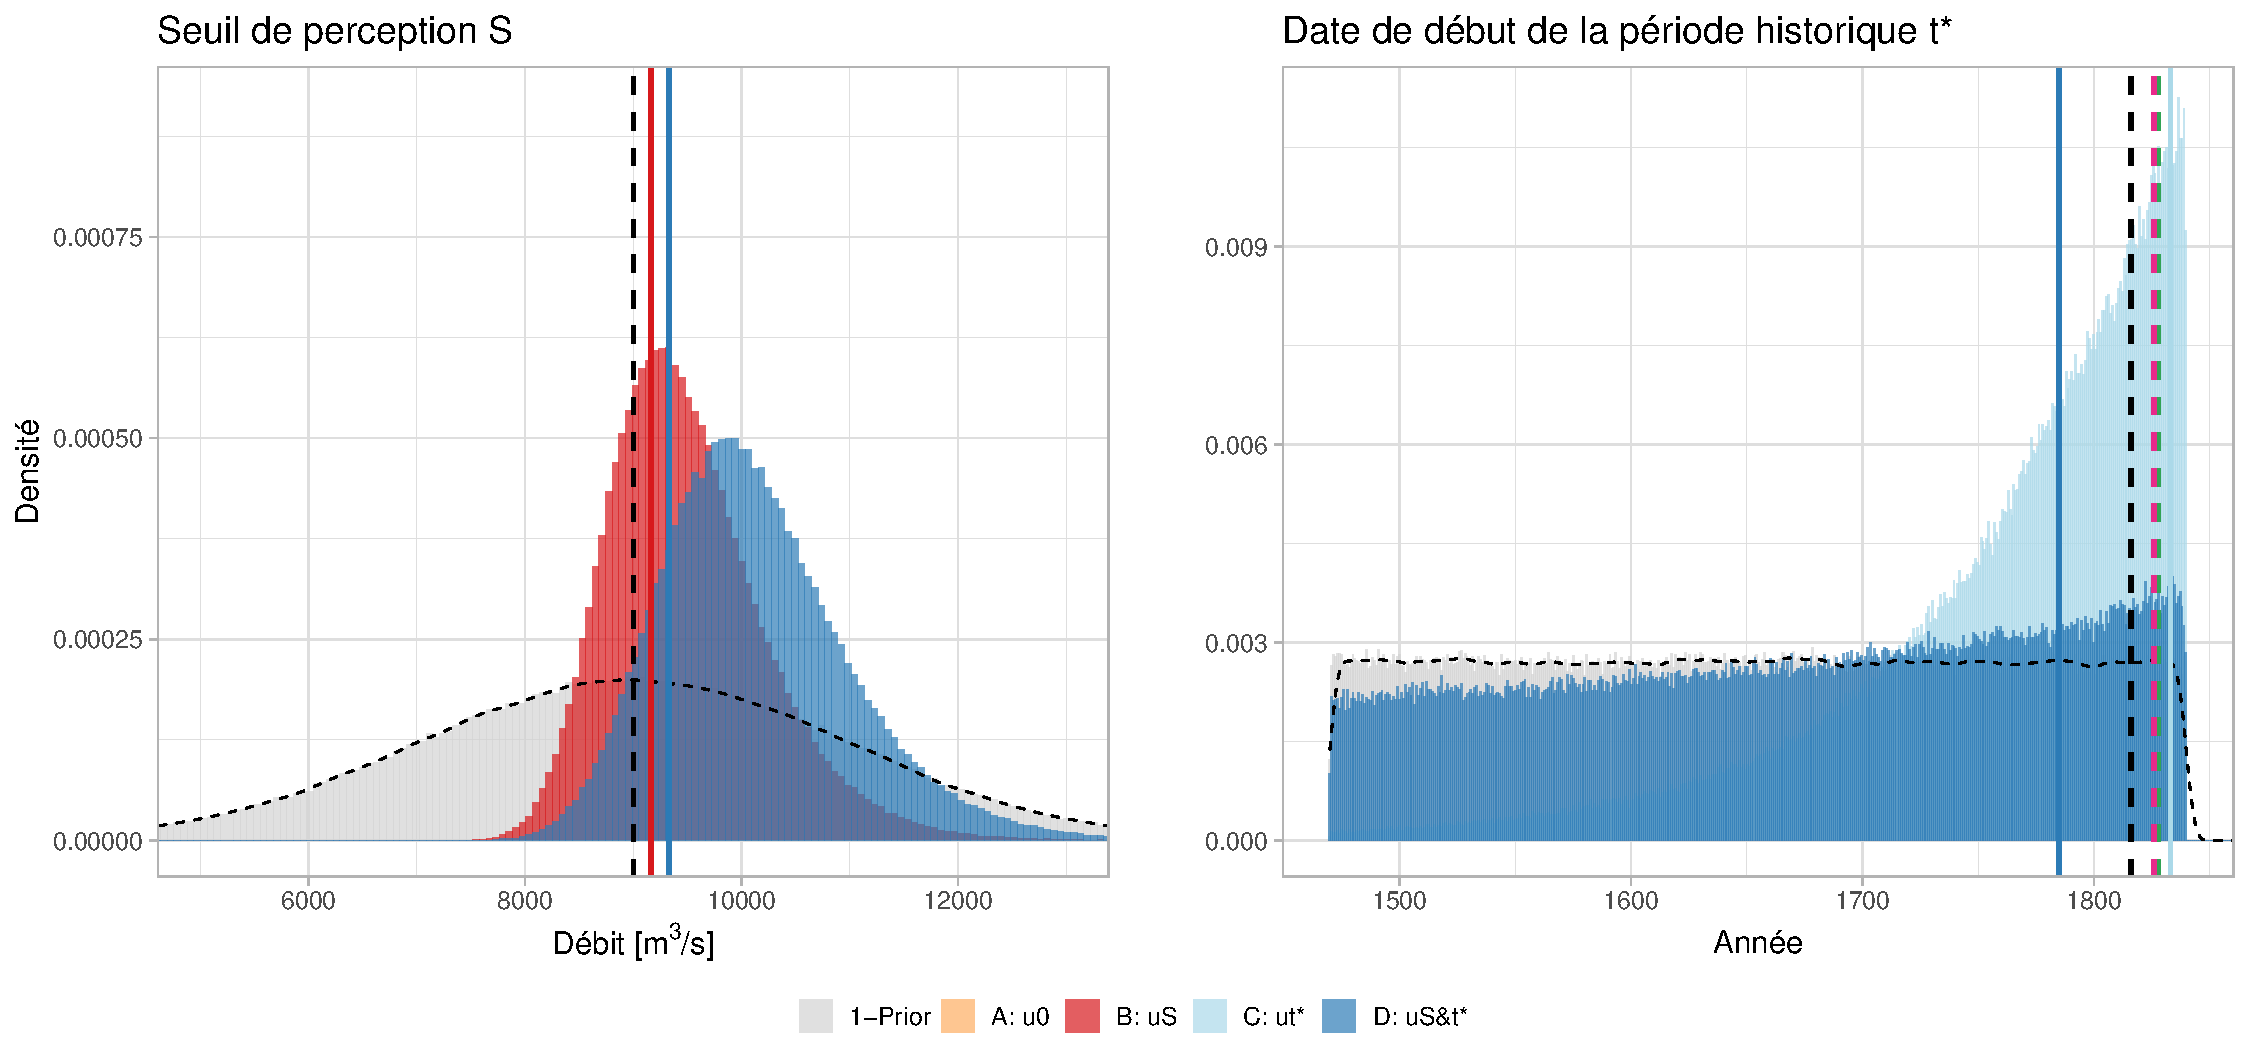
\includegraphics[width=.9\linewidth]{Chapitre4/Figures/Params_Artif2.pdf}	
		\caption{Distributions a priori et a posteriori pour le seuil de perception (gauche) et la date de début de la période historique (droite). Les droites verticales pleines représentent l'estimation maxpost du paramètre pour chacun des modèles et les droites en pointillés noirs représentent les valeurs de référence. Les droites verticales en pointillés vert et rose représentent respectivement les estimations de $t^{*}$ par la méthode de \citet{prosdocimi_german_2018} et la méthode de la période de retour du seuil $S$.}
		\label{fig:Params_Artif2}
	\end{figure}
	
	\subsubsection{Quel est l'impact de la méconnaissance de la durée de la période historique sur l'estimation des quantiles ?}	
	
	\paragraph{} Le modèle C permet de représenter la méconnaissance de la durée de la période historique, qui est l'un des deux paramètres de la loi binomiale utilisée ici pour modéliser le nombre d'occurrences de crues supérieures à un seuil. Sur la figure \ref{fig:Barplot_Artif2}, les estimations maxpost des quantiles pour le modèle C ont des valeurs légèrement supérieures aux estimations du modèle A. Cette légère sur-estimation provient d'une durée de période historique sous-estimée par le modèle, visible sur la figure \ref{fig:Params_Artif2} (droite). En effet, la date maxpost est l'année 1833, alors que la chronique débute réellement en 1816. Cette sous-estimation de 16 ans peut s'expliquer par une fréquence des crues supérieures au seuil $S4$ plus importante au cours de la période continue (4 crues / 50 ans = 0.08 crues/an) qu'au cours de la période historique (10 crues / 153 ans = 0.065 crues/an). Ce déséquilibre reflète l'existence d'oscillations dans la fréquence d'occurrence des crues dues à la variabilité d'échantillonnage, malgré le fait qu'aucune non-stationnarité des données n'ait été détectée par les tests à la section \ref{subsec:homog}. Il faut également noter que la distribution a posteriori pour le modèle C (figure \ref{fig:Params_Artif2}, droite) est largement réduite par rapport à l'a priori, et présente une forme très asymétrique. La distribution connait un maximum entre 1820 et 1840. Même si la valeur maxpost de $t^*$ est relativement éloignée de la vraie valeur (17 ans), la distribution a posteriori converge vers des valeurs cohérentes par rapport à l'a priori très peu informatif qui a été donné. 	 
	
	\paragraph{} L'incertitude autour des quantiles estimée par le modèle C est très similaire à celle estimée par le modèle A (figure \ref{fig:Barplot_Artif2}), de même que la distribution du paramètre de forme (figure \ref{fig:Shape_Artif2}). Une forte méconnaissance de la durée de la période historique n'a donc que peu d'impact sur la précision de l'estimation des quantiles, contrairement à la méconnaissance du seuil de perception.
	
	\subsubsection{Quel est l'impact de la méconnaissance du seuil de perception et de la durée de la période historique sur l'estimation des quantiles ?}	
	
	\paragraph{} Représenter la méconnaissance autour de $S$ et $n$ en même temps dans le modèle probabiliste paraît être la solution la plus raisonnable dans certains cas, notamment pour des événements très anciens et mal connus. Le modèle D est ici utilisé à cet effet. Les quantiles maxpost estimés dans la figure \ref{fig:Barplot_Artif2} pour le modèle D semblent cohérents avec les valeurs de référence. En revanche, la largeur de l'intervalle de confiance est importante et se situe entre celle du modèle B et du modèle C. Même si l'estimation est plus précise que celle du modèle GEV sur l'échantillon 1970-2020, elle reste imprécise pour la crue millénale. L'observation des paramètres a posteriori sur la figure \ref{fig:Params_Artif2} permet de comprendre l'origine de cette large incertitude. La distribution du seuil de perception, bien que centrée a proximité de la vraie valeur (maxpost à 9331 m\textsuperscript{3}/s), est très large (écart type = 883 m\textsuperscript{3}/s). Le seuil de perception parait ici un peu moins bien estimé que par le modèle B (écart type = 729 m\textsuperscript{3}/s). La date de début de la période historique est elle encore plus difficilement estimée, notamment en comparaison avec l'estimation du modèle C. On remarque que la distribution a posteriori est très similaire à celle de l'a priori, même si elle est légèrement asymétrique et marque un maximum non loin de la vraie valeur (l'année 1816). Cependant, les quantiles présentent une plus faible incertitude pour le modèle D que pour le modèle B. Cela provient de corrélations entre les paramètres qui peuvent être observées sur la figure \ref{fig:ScatterD_Artif2}. On remarque notamment une assez bonne corrélation entre la durée de la période historique $n$ et le seuil de perception $S$, ainsi qu'entre le seuil de perception et le paramètre de forme $\xi$. Il est donc complexe d'identifier ces paramètres séparément. Une élicitation plus précise de leurs a priori sera certainement nécessaire.
	
	\begin{figure}[h]
		\centering
		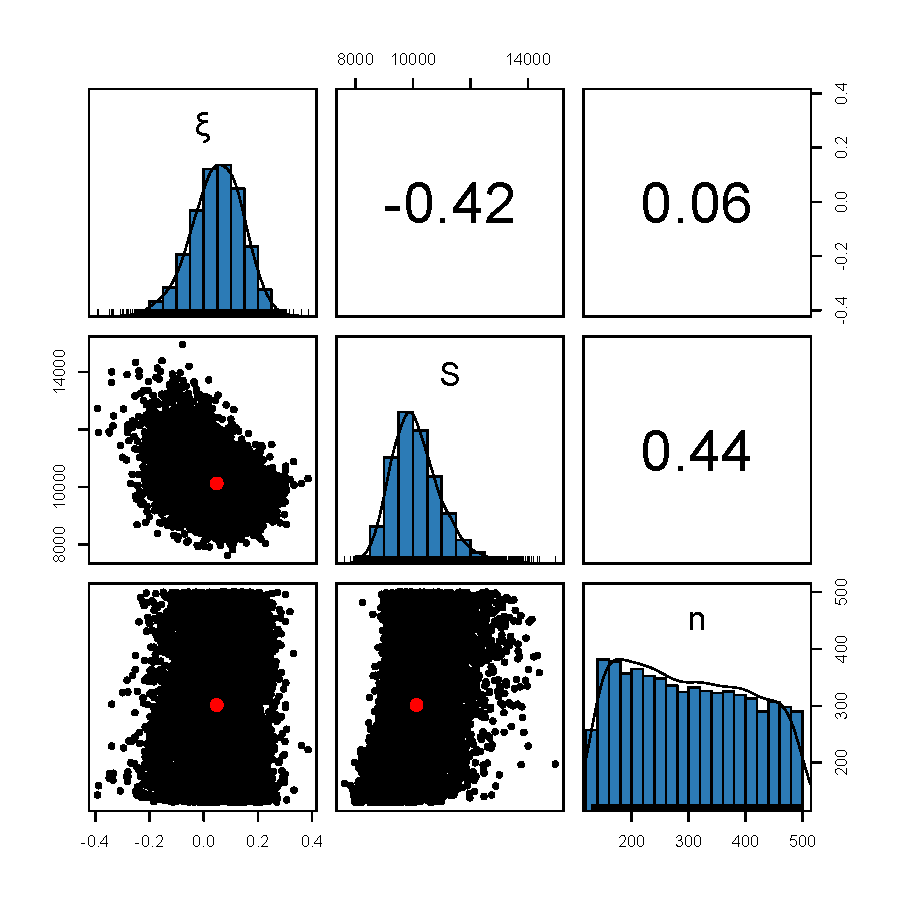
\includegraphics[width=.7\linewidth]{Chapitre4/Figures/ScatterD_Artif2.pdf}
		\caption{Scatterplots des distributions a posteriori de trois paramètres du modèle D pour l'échantillon 4 : le paramètre de forme $\xi$ (sans unité), le seuil de perception $S$ (en m\textsuperscript{3}/s) et la durée de la période historique $n$ (en années). Les nombres inscrits dans les cases supérieures correspondent aux corrélations entre les paramètres et les points rouges correspondent aux médianes.}
		\label{fig:ScatterD_Artif2}
	\end{figure}
		
\FloatBarrier

	\subsubsection{Quel est l'apport de la connaissance du débit des crues historiques ?}

	\paragraph{} Les modèles A, B, C et D n'utilisent que l'information du nombre de dépassements $k$ d'un seuil de perception $S$ pendant une durée $n$. Le débit des crues historiques ayant dépassé le seuil est donc ignoré. Le modèle E permet de prendre en compte cette donnée de débit ainsi que l'incertitude correspondant à chaque crue. Il a été appliqué à l'échantillon 4 du tableau \ref{tab:Echantillons} en considérant l'incertitude des débits de la période historique (1816-1969) calculée au chapitre \ref{chap:ch3}.
	
	
	\begin{figure}[h]
		\centering
		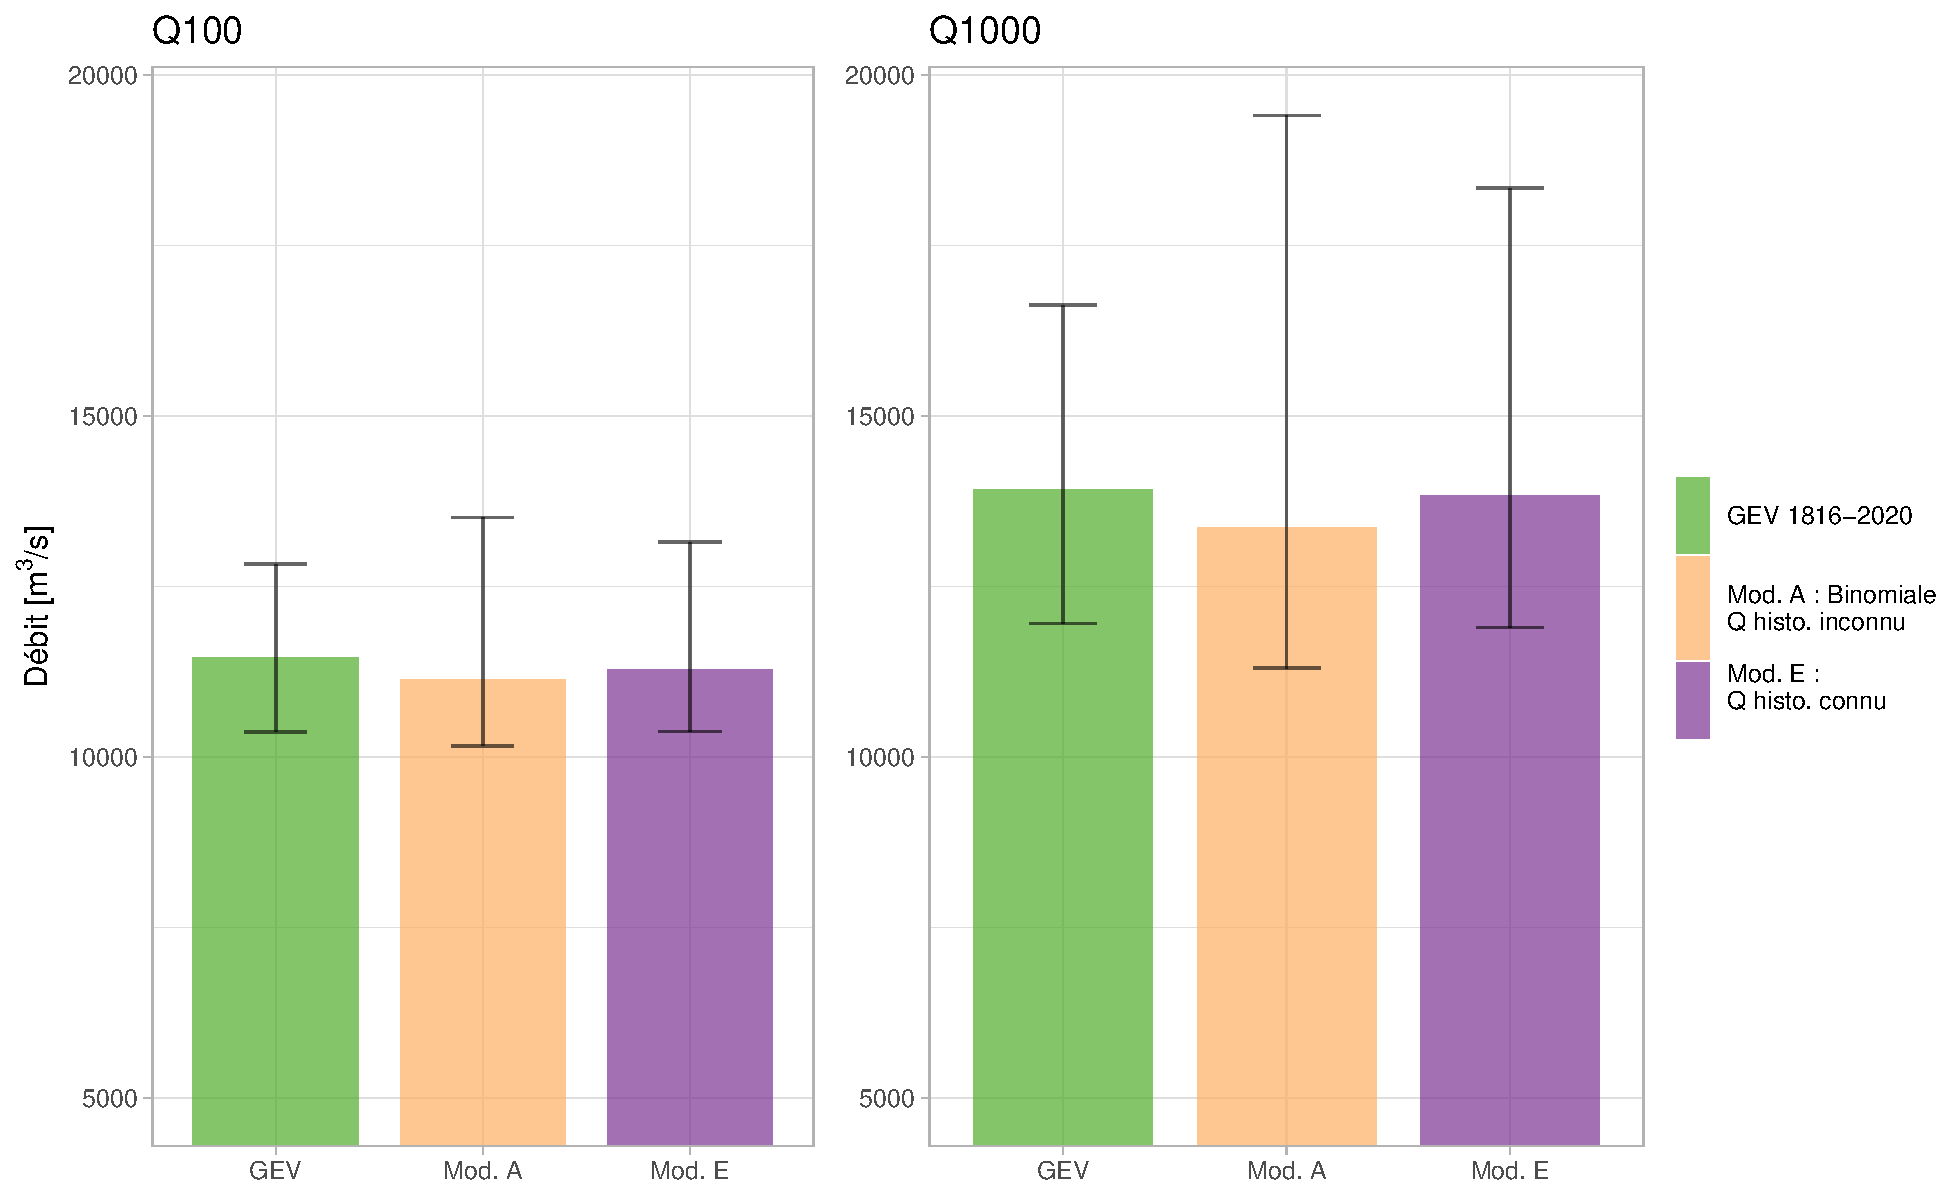
\includegraphics[width=.8\linewidth]{Chapitre4/Figures/Barplots_QX_censure.pdf}
		\caption{Estimations maxpost et incertitudes à 95\% pour Q100 et Q1000 pour 3 modèles appliqués à l'échantillon 4 (1816-2020 dégradé, $S4$). Le modèle A n'utilise que le nombre de dépassements du seuil de perception, alors que le modèle E considère le débit des crues historiques (et son incertitude) ayant dépassé le seuil $S$.}
		\label{fig:CensureArtif}
	\end{figure}
	
%	\begin{table}[h]
%		\centering
%		\caption{Résultats maxpost et incertitudes pour trois modèles appliqués à l'échantillon 4. Q100 et Q1000 représentent respectivement le débit des crues centennales et millénales. Les écarts type des distributions a posteriori sont représentés par les colonnes débutant par la lettre "u". \textcolor{red}{A BASCULER DANS LE TABLEAU 2}}
%		\label{tab:ResCensure}
%%		\resizebox{\columnwidth}{!}{%
%		\begin{tabular}{|c|c|c|c|c|}
%			\hline
%			Modèle        & Q100 [m\textsuperscript{3}/s] & uQ100 [m\textsuperscript{3}/s] & Q1000 [m\textsuperscript{3}/s] & uQ1000 [m\textsuperscript{3}/s] \\ \hline
%			GEV 1816-2020 & 11451 & 687   & 13919 & 1351   \\ \hline
%			A             & 11132 & 1189  & 13367 & 3019   \\ \hline
%			E       & 11286 & 932   & 13827 & 2255   \\ \hline
%		\end{tabular}%}
%		
%	\end{table}
%	
	\paragraph{}
	Les résultats sont présentés dans la figure \ref{fig:CensureArtif} et le tableau \ref{tab:ResArtif2}. On constate une diminution de l'incertitude d'environ 25\% autour du Q1000 pour le modèle E (avec un écart type de 2255 [m\textsuperscript{3}/s] pour Q1000) par rapport au modèle binomial A (écart type de 3019 [m\textsuperscript{3}/s] pour Q1000). En revanche, l'incertitude du modèle E reste environ 65\% supérieure à celle du modèle GEV 1816-2020 pour Q1000. La connaissance du débit des crues historiques, bien qu'elle ne soit pas une condition nécessaire à l'utilisation de données pré-enregistrements systématiques, permet donc de réduire l'incertitude autour des quantiles extrêmes. Cette incertitude reste en revanche supérieure à celle du modèle GEV pour lequel le débit maximum annuel de toutes les années de l'échantillon (historique + continu) est connu.	

	\subsubsection{Discussion intermédiaire}
	
	\paragraph{} L'utilisation des modèles décrits dans la section \ref{sec:MethodoCh3} sur un échantillon artificiellement dégradé et dont les caractéristiques sont parfaitement connues permet d'évaluer la performance des modèles et l'impact de la méconnaissance du seuil de perception $S$ et de la durée de la période historique $n$ sur l'estimation des quantiles extrêmes. On constate en observant les résultats que la méconnaissance du seuil de perception a un plus fort impact sur l'incertitude des résultats que la méconnaissance de la durée de la période historique. Même si les distributions a posteriori du seuil de perception pour les modèles B et D sont centrées a proximité de la vraie valeur (9000 m\textsuperscript{3}/s), l'incertitude résultant de la détermination du seuil a un fort impact sur l'incertitude des quantiles. En revanche, l'estimation de la durée de la période historique dans le cas des modèles C et D semble elle aussi relativement peu précise, mais n'impacte que peu l'incertitude des résultats si on compare ces derniers à ceux du modèle A. Cela est dû à des corrélations entre paramètres (figure \ref{fig:ScatterD_Artif2}) qui entraînent une réduction de l'incertitude finale.
	 
	\paragraph{} Ces premiers résultats démontrent que l'incertitude des quantiles peut être sous-estimée	lorsque l'on considère seuil de perception et durée de période historique comme étant bien connus alors que ce n'est pas le cas. Les modèles utilisés ici permettent de prendre en compte cette méconnaissance dans l'estimation des quantiles extrêmes. On pourra par la suite les appliquer au cas réel de l'échantillon de crues de la période 1500-2020 à Beaucaire, dont le seuil de perception et la durée de période historique ne sont pas connus précisément. Si les a priori utilisés jusqu'ici étaient peu informatifs afin de comprendre les performances du modèle, ils devront être élicités plus précisément par la suite afin d'obtenir des résultats qui reflètent davantage la connaissance/méconnaissance du seuil de perception et de la durée de la période historique.
		
	\paragraph{} Enfin, la comparaison du modèle A pour lequel seul le nombre de dépassements du seuil de perception est connu avec le modèle E pour lequel le débit des crues historiques est connu (ainsi que l'incertitude autour de ces débits) a permis de démontrer l'intérêt de reconstituer le débit des crues historiques. Néanmoins, ces résultats ne sont valables que pour le seuil de perception $S4$ utilisé ici. Plusieurs études (notamment \citet{stedinger_flood_1986} et \citet{payrastre_usefulness_2011}) ont démontré que l'écart d'incertitude entre les résultats de ces deux types de modèles tendait à se réduire à mesure que la période de retour du seuil de perception tendait vers environ 50 ans, jusqu'à devenir nul au delà de cette magnitude. Cela encourage donc l'utilisation du nombre de dépassements d'un seuil de perception lorsqu'il n'est pas possible d'avoir de meilleure information sur la période historique.
	
	\subsection{Application à la période 1500-2020}
	\label{subsec:Results1500}
	
	\paragraph{} Les modèles A, B, C et D de la section \ref{sec:MethodoCh3} ont été appliqués à l'échantillon 2 (1500-2020, seuil $S4$). Les estimations centennales et millénales sont présentés dans la figure \ref{fig:BarplotC4} et sont comparés au modèle GEV sur l'échantillon continu 1816-2020. On retrouve également ces résultats dans le tableau \ref{tab:ResC4}, accompagnés des valeurs a posteriori de certains paramètres du modèle. Les distributions a posteriori de $S$ et $t^{*}$ sont également représentées dans la figure \ref{fig:Params_C4}.
	
	
	\begin{figure}[h]
		\centering
		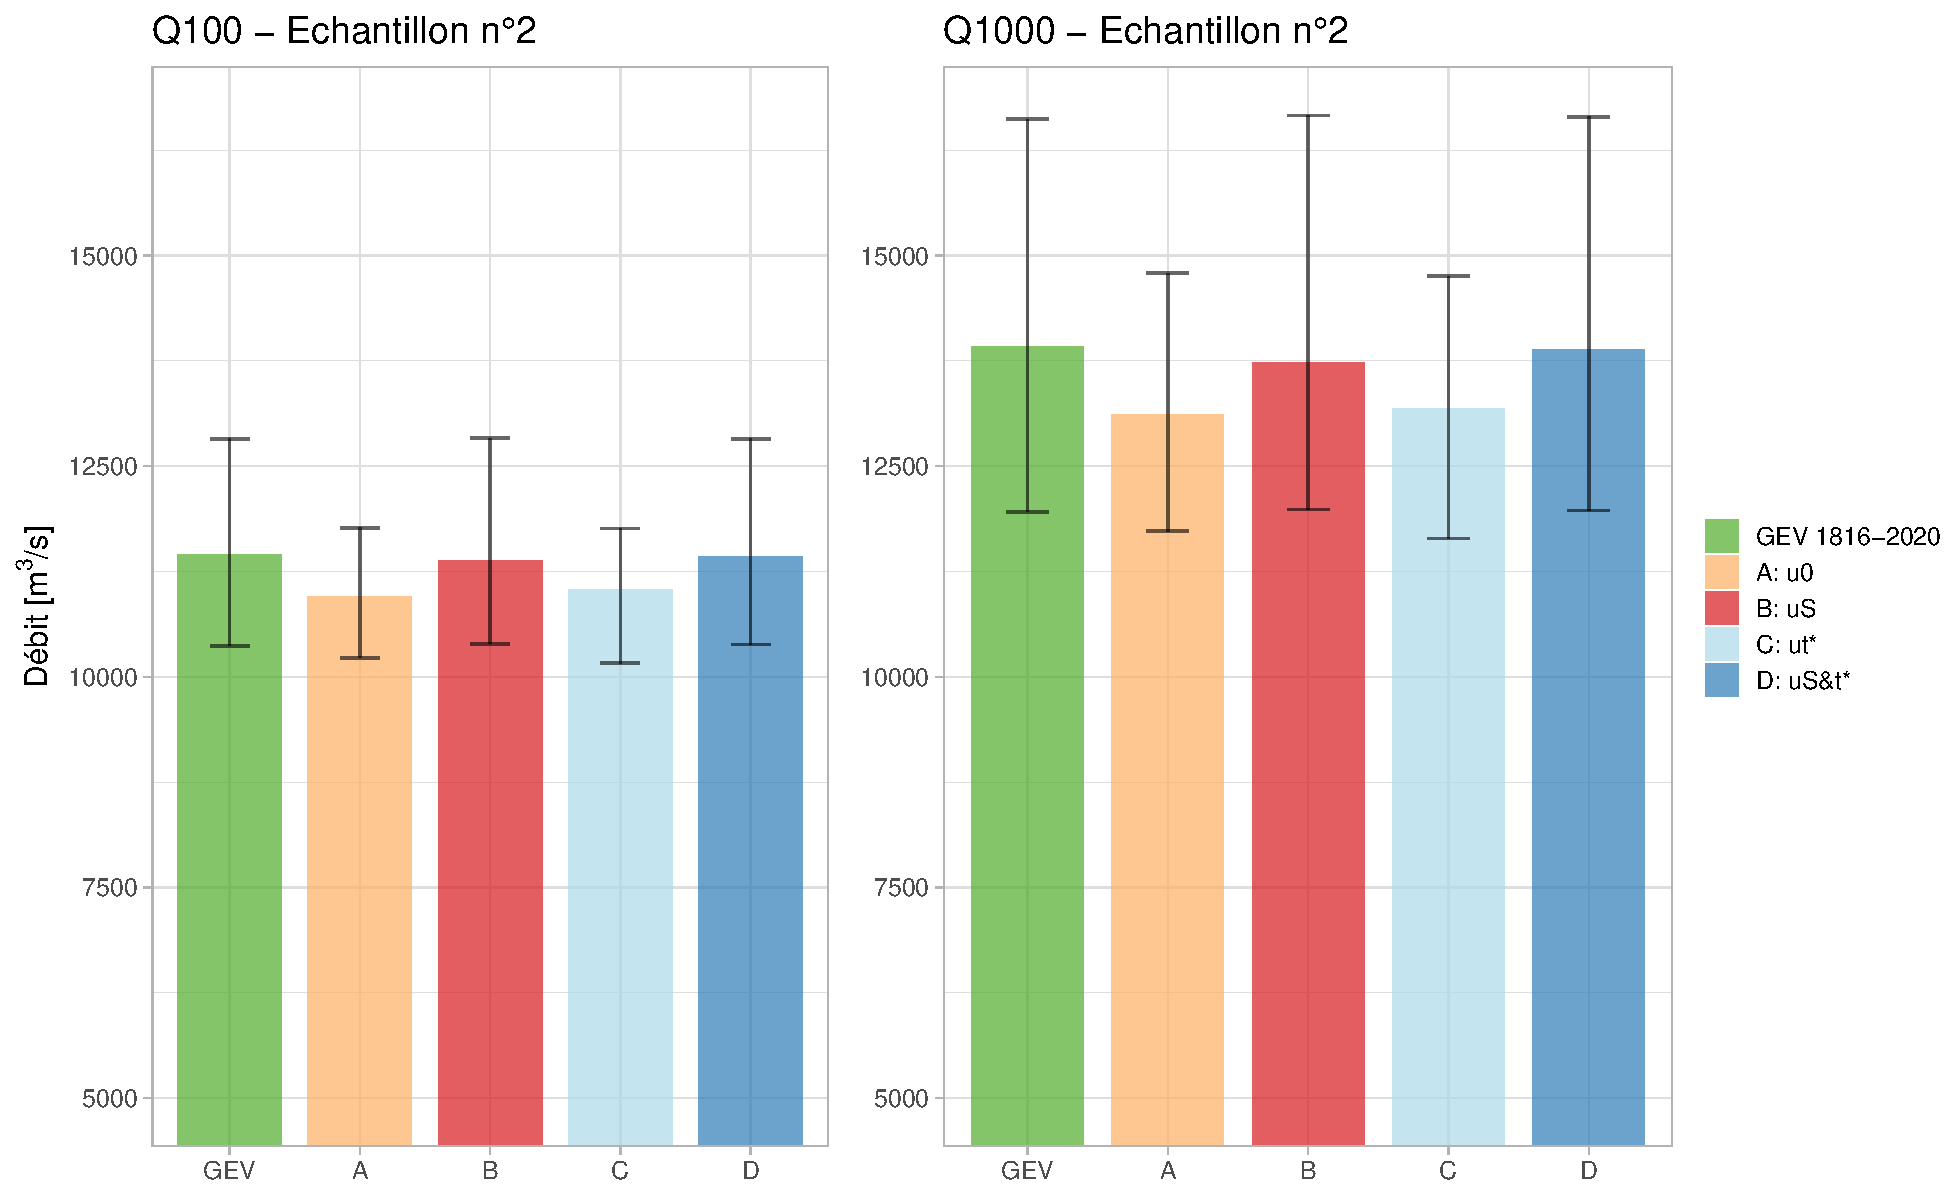
\includegraphics[width=.8\linewidth]{Chapitre4/Figures/Barplots_QX_C4.pdf}
		\caption{Estimations maxpost et incertitudes à 95\% pour Q100 et Q1000 par 5 modèles différents pour l'échantillon 2 (1500-2020, $S4$)}
		\label{fig:BarplotC4}
	\end{figure}
	
		\begin{table}[h]
	\centering
	\caption{Résultats maxpost et incertitudes de 6 modèles pour l'échantillon 2. Le modèle $D^*$ représente les résultats du modèle D avec des a priori plus informatifs (section \ref{subsec:D*}). Q100 et Q1000 représentent respectivement le débit des crues centennales et millénales, $\xi$ le paramètre de forme de la distribution GEV, $S$ le seuil de perception et $t^{*}$ la date de début de la période historique. Les écarts type des distributions a posteriori sont représentés par les colonnes débutant par la lettre "u".}
		\label{tab:ResC4}
	\resizebox{\columnwidth}{!}{%
		\begin{tabular}{|c|c|c|c|c|c|c|c|c|c|c|}
		\hline
Modèle & Q100 [m\textsuperscript{3}/s] & uQ100 [m\textsuperscript{3}/s] & Q1000 [m\textsuperscript{3}/s] & uQ1000 [m\textsuperscript{3}/s] & $\xi$ & $u\xi$ & $S$ [m\textsuperscript{3}/s] & $uS$ [m\textsuperscript{3}/s] & $t^{*}$ & $ut^{*}$ \\ \hline
GEV 1816-2020 & 11451 & 687   & 13919 & 1351   & 0,058 & 0,044  & X    & X    & X    & X \\ \hline
A             & 10977 & 391   & 13149 & 816    & 0,073 & 0,038  & 9000 & X    & 1500 & X \\ \hline
B             & 11438 & 698   & 13875 & 1391   & 0,06  & 0,044  & 9628 & 504  & 1500 & X \\ \hline
C             & 10975 & 395   & 13139 & 809    & 0,074 & 0,038  & 9000 & X    & 1527 & 44 \\ \hline
D             & 11336 & 745   & 13721 & 1467   & 0,061 & 0,044  & 9613 & 551  & 1529 & 62 \\ \hline
$D^*$         & 11118 & 585   & 13421 & 1110   & 0.063 & 0.040  & 9386 & 334  & 1526 & 17 \\ \hline
		\end{tabular}}

	\end{table}
	

	\begin{figure}[h]
		\centering
		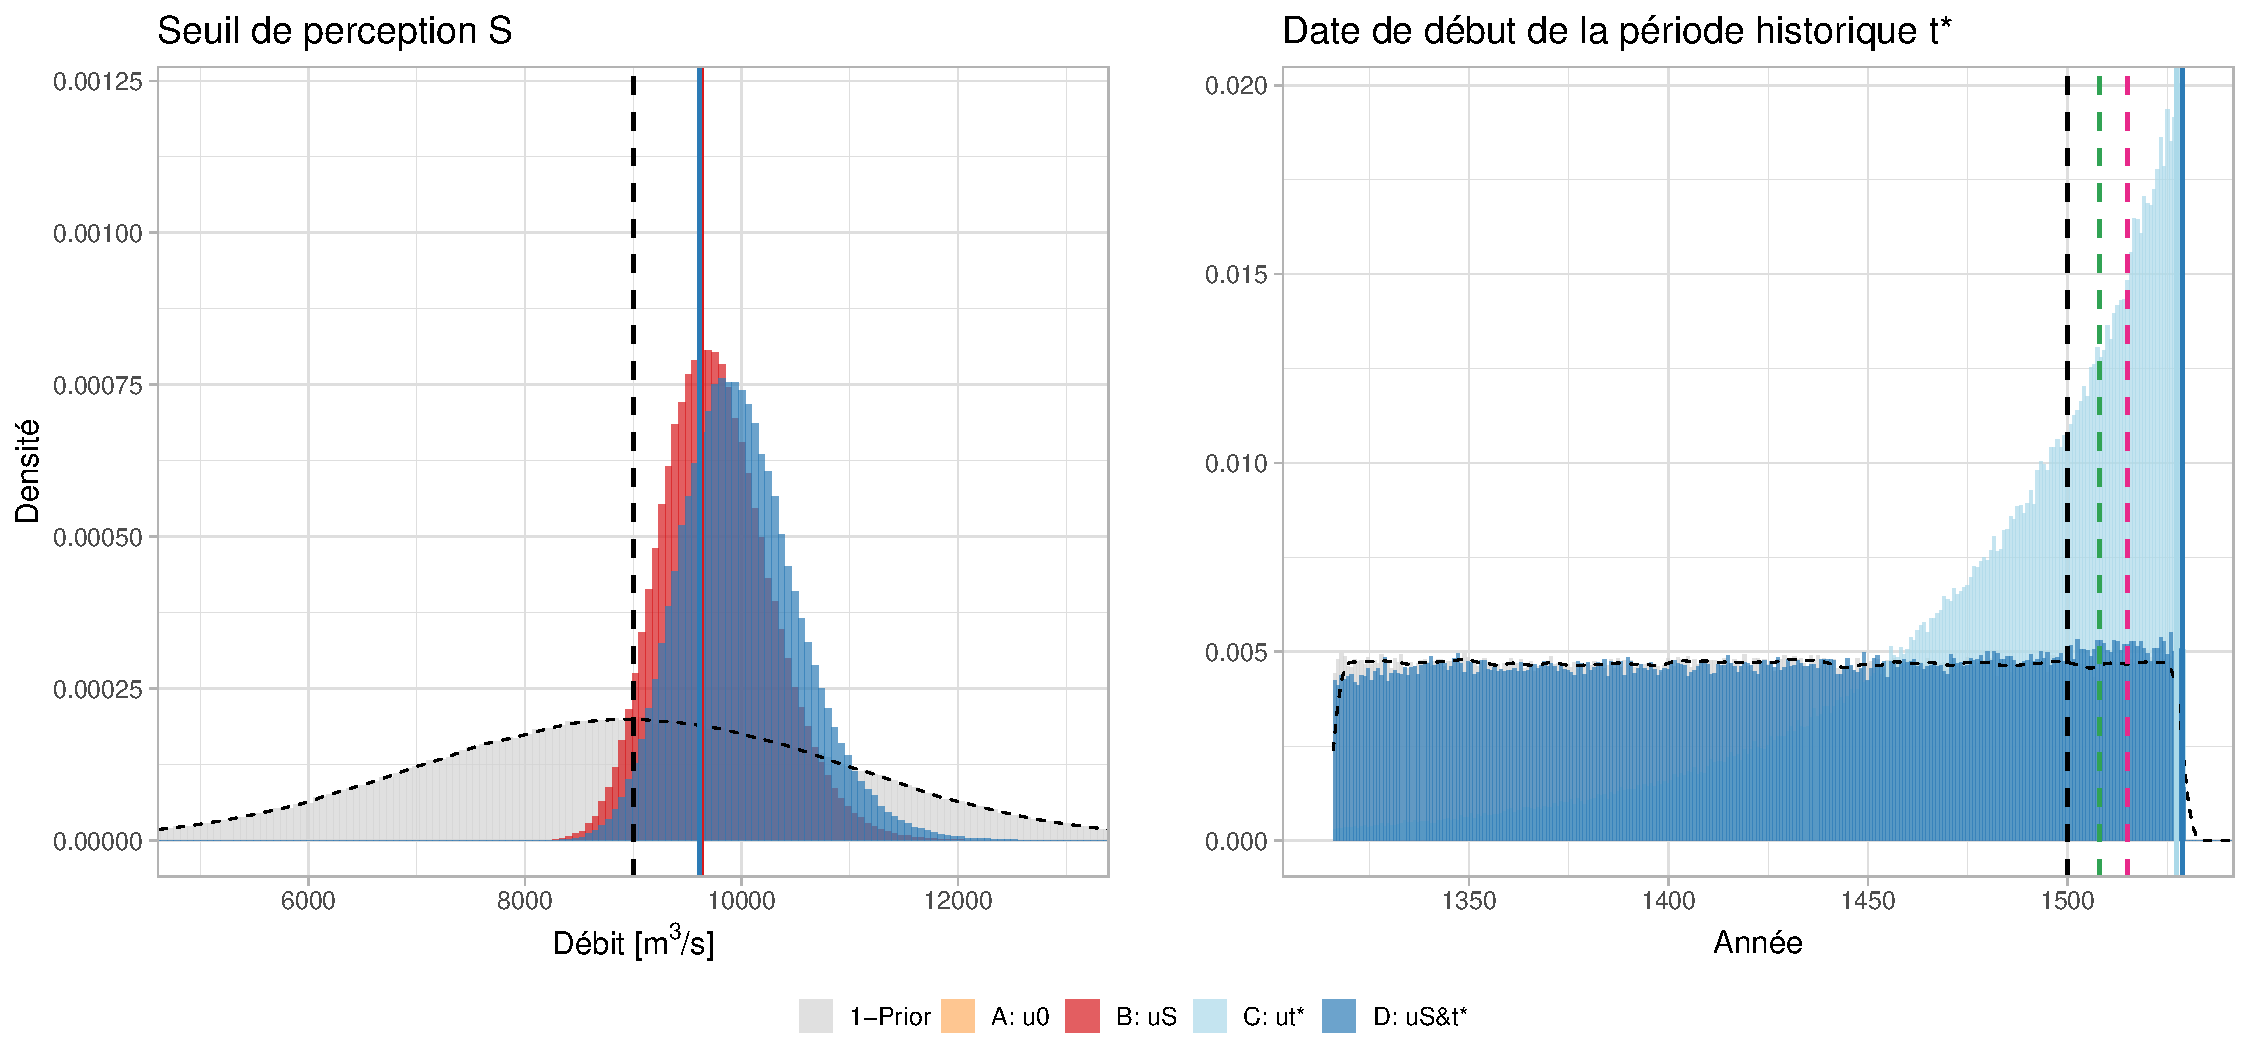
\includegraphics[width=.9\linewidth]{Chapitre4/Figures/Params_C4.pdf}	
		\caption{Distributions a priori et a posteriori pour le seuil de perception (gauche) et la date de début de la période historique (droite). Les droites verticales pleines représentent l'estimation maxpost du paramètre pour chacun des modèles et les droites en pointillés noirs représentent les valeurs de référence. Les droites verticales en pointillés vert et rose représentent respectivement les estimations de $t^{*}$ par la méthode de \citet{prosdocimi_german_2018} et par la méthode de la période de retour du seuil $S$.}
		\label{fig:Params_C4}
	\end{figure}

		\subsubsection{Comparaison des modèles historiques}
		
		
	\paragraph{} Tout d'abord, on observe bien évidemment des résultats moins incertains que pour l'échantillon dégradé (figure \ref{fig:Barplot_Artif2}). L'incertitude des résultats (pour Q100 et Q1000) des modèles GEV-Binomiale est au moins équivalente à celle de la référence (GEV 1816-2020), voire plus faible pour les modèles supposant un seuil de perception connu (A et C). Pour ces mêmes modèles, les quantiles maxpost sont légèrement plus faibles (d'environ 5\%) que ceux de la référence (tableau \ref{tab:ResC4}). De la même manière qu'avec l'échantillon dégradé, on observe ici que la méconnaissance du seuil de perception (B et D) a plus d'impact sur l'incertitude des résultats que la méconnaissance de la durée de la période historique (C et D). 
	
	\paragraph{} On peut notamment expliquer ces différences en observant les distributions a posteriori des paramètres $S$ et $t^{*}$ (figure \ref{fig:Params_C4}). Tout d'abord, ces distributions sont très similaires à celles observées pour l'échantillon 4 (pour des a priori équivalents). Les écarts-type a posteriori pour le seuil de perception (modèles B et D) sont relativement faibles (environ 500 m\textsuperscript{3}/s pour les deux modèles) et les distributions sont centrées vers des valeurs supérieures à la valeur a priori de 9000 m\textsuperscript{3}/s (valeurs maxpost autour de 9600 m\textsuperscript{3}/s, tableau \ref{tab:ResC4}). La date de début de période historique a posteriori pour le modèle C semble à nouveau bien mieux estimée que celle du modèle D, dont la distribution a posteriori est très proche de l'a priori. Pour les deux modèles, les estimations maxpost de $t^*$ sont supérieures de pratiquement 30 ans à la valeur supposée de 1500. On constate notamment que la distribution a posteriori pour le modèle C connait un maximum pour l'année 1529, qui correspond à la date de la première crue de l'échantillon. 
	
	\paragraph{} Cette tendance vers un seuil plus important et une période historique plus courte pourrait être le symptôme d'une non-exhaustivité des crues dans l'échantillon C4 de la base HISTRHÔNE, et ce malgré qu'aucune non-homogénéité de la fréquence des crues supérieures au seuil $S4$ n'ait été détectée (section \ref{subsec:homog}). À nouveau, on peut comparer la fréquence d'occurrence des crues supérieures au seuil $S4$ respective à chacun des deux échantillons. Pour l'échantillon historique, on observe 13 crues pour une durée de 315 ans, soit une fréquence de 0.041 crues/an. Pour l'échantillon continu, on observe 14 crues sur une durée de 204 ans, soit une fréquence de 0.068 crues/an. C'est donc ce déséquilibre en faveur de la période continue, qu'il soit dû à la variabilité d'échantillonnage, à la variabilité climatique, ou à la non-exhaustivité des données historiques, qui entraine l'estimation de seuils de perception plus importants ou de durées historiques plus courtes. L'homogénéité "interne" des deux échantillons a pourtant été validée (section \ref{subsec:homog}), mais cela ne garantit pas une homogénéité inter-échantillons. De plus, il est possible qu'un échantillon soit considéré homogène sans qu'il soit pour autant exhaustif : par exemple la proportion de crues "oubliées" peut être stable dans le temps.
	
	
	\paragraph{} Dans le cas de Beaucaire, l'utilisation du nombre d'occurrences de crues historiques supérieures à un seuil ne permet donc de réduire l'incertitude autour des quantiles estimés que lorsque le seuil de perception est supposé parfaitement connu. L'utilisation d'a priori plus informatifs permettrait probablement d'obtenir des résultats moins incertains et plus réalistes quant à la connaissance du seuil de perception et de la durée de la période historique. Il faut également retenir qu'un doute demeure sur l'exhaustivité de l'échantillon historique ou sur l'homogénéité inter-échantillons.
	 
	 \subsubsection{Estimation des quantiles à Beaucaire (1500-2020) avec des a priori plus informatifs}
	 \label{subsec:D*}

	\paragraph{} Après analyse des résultats des modèles pour différents échantillons, il apparait que l'estimation la plus prudente des quantiles de crues à Beaucaire (1500-2020) consiste à utiliser le modèle D ($S$ et $n$ incertains) en parallèle d'une élicitation d'a priori relativement informatifs. De plus, \citet{stedinger_flood_1986} et \citet{payrastre_usefulness_2011} décrivent qu'un modèle binomial apporte des résultats aussi informatifs qu'un modèle pour lequel le débit des crues historiques est connu si le seuil de perception est suffisamment grand. L'utilisation de l'échantillon correspondant au seuil de perception le plus grand ($S4$) semble donc être plus intéressante. La distribution a priori du seuil est à nouveau supposée gaussienne et centrée sur la valeur de 9000 m\textsuperscript{3}/s, en accord avec les estimations de \citet{pichard_hydro-climatology_2017} et des résultats du chapitre \ref{chap:ch2}. L'écart type de la distribution est fixé à 500 m\textsuperscript{3}/s, ce qui le rend l'a priori plus informatif que lors des calculs précédents. En ce qui concerne la date de début de la période historique $t^{*}$, une distribution uniforme est utilisée. La borne supérieure de la distribution reste fixée à la date de la première crue de la série (en 1529). En revanche, la borne inférieure est affectée à deux fois la durée entre la date de la première crue (1529) et la valeur supposée de $t^{*}$ (1500), soit 58 ans. La borne inférieure de la distribution a priori est donc l'année 1471. La valeur théorique calculée en utilisant la méthode proposée par \citet{prosdocimi_german_2018} est 1510, elle est bien comprise dans la distribution a priori. Il en est de même pour la valeur de $t^{*}$ correspondant à la différence entre la période de retour du seuil de perception $S4$ (environ 15 ans) et la date de la première crue, ce qui correspond à l'année 1515. L'application du modèle D avec ces a priori plus informatifs correspondra au terme $D^*$ dans les sections suivantes

	\begin{figure}[h]
		\centering
		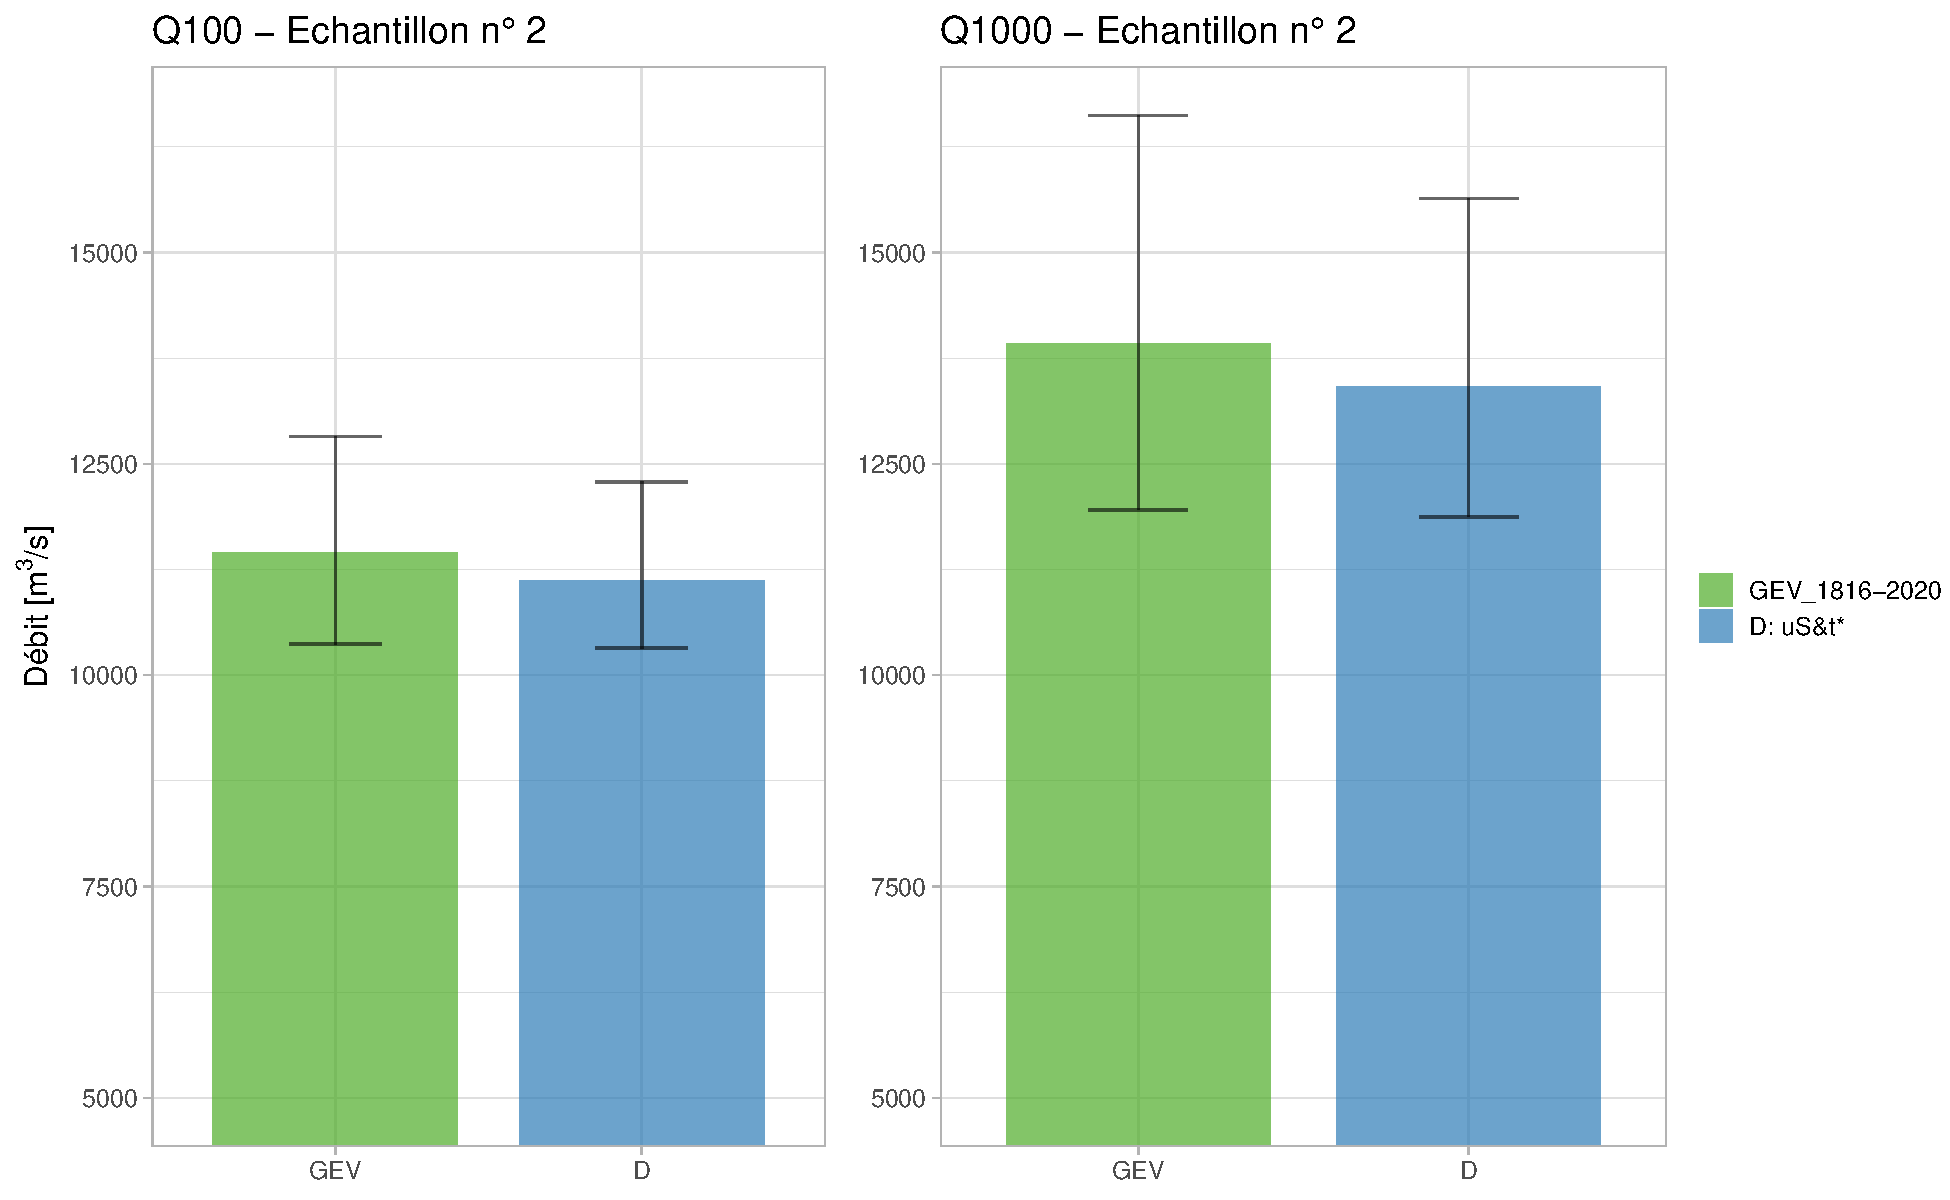
\includegraphics[width=.8\linewidth]{Chapitre4/Figures/Barplots_QX_C4short.pdf}
		\caption{Estimations maxpost et incertitudes à 95\% pour Q100 et Q1000 des modèles GEV 1816-2020 et $D^*$ pour l'échantillon 2 (1500-2020, $S4$) après révision des distributions a priori de $S4$ et $n$.}
		\label{fig:BarplotC4short}
	\end{figure}

	\paragraph{} Les résultats du modèle $D^*$ sont présentés dans la figure \ref{fig:BarplotC4short} ainsi que dans le tableau \ref{tab:ResC4} où ils sont comparés avec les estimations de référence (GEV 1816-2020). On constate que l'incertitude des quantiles est réduite d'environ 15\% par rapport à la référence pour Q100 et Q1000. Les estimations maxpost sont également réduites d'environ 3\% pour les deux périodes de retour. L'utilisation des crues historiques apparait donc pertinente pour réduire l'incertitude des quantiles, même dans le cas où $S$ et $n$ sont incertains. On peut également noter que l'élicitation d'a priori plus informatifs a permis de réduire d'environ 25\% l'écart type de la distribution a posteriori pour Q1000 (comparaison de D et $D^*$). 

%	\begin{table}[h]
%	\centering
%	\caption{Résultats maxpost et incertitudes de 2 modèles pour l'échantillon 2 après révision des distributions a priori de $S4$ et $n$. Q100 et Q1000 représentent respectivement le débit des crues centennales et millénales, $\xi$ le paramètre de forme de la distribution GEV, $S$ le seuil de perception et $t^{*}$ la date de début de la période historique. Les écarts type des distributions a posteriori sont représentés par les colonnes débutant par la lettre "u".}
%	\label{tab:ResC4short}
%	\resizebox{\columnwidth}{!}{%
%		\begin{tabular}{|c|c|c|c|c|c|c|c|c|c|c|}
%		\hline
%Modèle & Q100 [m\textsuperscript{3}/s] & uQ100 [m\textsuperscript{3}/s] & Q1000 [m\textsuperscript{3}/s] & uQ1000 [m\textsuperscript{3}/s] & $\xi$ & $u\xi$ & $S$ [m\textsuperscript{3}/s] & $uS$ [m\textsuperscript{3}/s] & $t^{*}$ & $ut^{*}$ \\ \hline
%GEV 1816-2020 & 11451 & 687   & 13919 & 1351   & 0.058 & 0.044  & X    & X    & X    & X \\ \hline
%
%		\end{tabular}}
%
%	\end{table}
		
	\paragraph{} Les distributions a posteriori de $S$ et $t^{*}$ sont présentées dans la figure \ref{fig:Params_C4short}. Une fois de plus, la distribution a posteriori du seuil de perception est décalée vers des valeurs plus élevées que la valeur supposée de 9000 m\textsuperscript{3}/s, avec un seuil maxpost à 9386 m\textsuperscript{3}/s. La distribution a posteriori de $t^{*}$ est à nouveau très proche de la distribution a priori, avec une densité un peu plus élevée pour les années proches de la date de la première crue. L'estimation maxpost de $t^{*}$ est ici 1526, soit une durée de la période historique $n$ 26 ans plus courte qu'attendu. Cependant, le doute quant à l'exhaustivité de l'échantillon historique ou l'homogénéité inter-échantillons tel que décrit dans la section précédente.
			
	\begin{figure}[h]
		\centering
		\includegraphics[width=.9\linewidth]{Chapitre4/Figures/Params_C4short.pdf}	
		\caption{Distributions a priori et a posteriori pour le seuil de perception (gauche) et la date de début de la période historique (droite). Les droites verticales représentent l'estimation maxpost du paramètre de forme pour chacun des modèles. La droite verticale noire représente la date de début supposée de la chronique historique, ici 1500.}
		\label{fig:Params_C4short}
	\end{figure}
	
	\FloatBarrier
	
	\section{Discussion}
	\label{sec:Discussion}
	\paragraph{} L'intérêt de la valorisation des données historiques pour l'analyse fréquentielle des crues est connu et étudié depuis longtemps (\cite{benson_use_1950}; \cite{stedinger_flood_1986}). L'utilisation des données anciennes doit être accompagnée d'une estimation complète des incertitudes \citep{kjeldsen_documentary_2014}. Lors de l'utilisation d'un échantillon d'occurrences de crues supérieures à un seuil (le débit des crues historiques supérieures au seuil de perception n'est pas connu), la méconnaissance du seuil de perception et de la durée de la période historique est souvent négligée. Seule l'incertitude provenant de l'estimation des paramètres de la distribution choisie est généralement considérée. Plusieurs modèles sont proposés dans ce chapitre permettant de prendre en compte la méconnaissance autour de ces deux paramètres. La propagation de l'incertitude des débits de la période récente est également effectuée. 
	
	\paragraph{} Les modèles ont dans un premier temps été testés avec des a priori très peu informatifs et sur un échantillon continu artificiellement dégradé afin de se replacer dans un contexte historique. Ainsi, seuil de perception et durée de la période historique sont parfaitement connus. Les quantiles estimés ont été comparés avec les estimations d'un modèle GEV pour l'entièreté de la période (figure \ref{fig:Barplot_Artif2}). Il est apparu que considérer le seuil de perception comme étant incertain avait bien plus d'impact sur l'incertitude des résultats que considérer une méconnaissance sur la durée de la période historique. En revanche, quand ces deux paramètres sont considérés incertains en même temps, l'incertitude autour des quantiles est réduite par rapport au cas où seul le seuil est incertain. Une corrélation entre les distributions a posteriori de ces deux paramètres a été mise en évidence. Cette corrélation n'est pas surprenante étant donné que seuil et durée de la période historique sont par définition reliés : le nombre de dépassements du seuil de perception $k$ est à la fois dépendant du seuil $S$ et de la durée $n$. L'élicitation d'a priori plus informatifs pour ces deux paramètres est donc nécessaire. Bien que le seuil de perception soit un objet parfois difficile à cerner, il est donc possible de représenter sa méconnaissance à l'intérieur même du modèle probabiliste. Considérer que le seuil de perception est parfaitement connu lorsque ce n'est pas le cas peut mener à une importante sous-estimation de l'incertitude des quantiles, de même que pour la durée de la période historique, dans une moindre mesure. Dans le cas de cet échantillon dégradé, l'utilisation des données historiques permet de réduire l'incertitude des quantiles par rapport à la seule utilisation de l'échantillon continu (dégradé), et ce quelque soit l'hypothèse retenue concernant la méconnaissance de $S$ et $n$.
	
	\paragraph{} L'estimation du modèle binomial pour $S$ et $n$ connus (modèle A) a ensuite été comparée à une estimation pour laquelle le débit des crues historiques est connu et situé dans un intervalle (modèle E) pour l'échantillon dégradé (figure \ref{fig:CensureArtif}). L'incertitude des résultats du modèle E se situe entre celle du modèle A et celle du modèle GEV pour l'ensemble de la période. Dans ce cas précis, l'utilisation du débit des crues historiques s'est donc avérée légèrement plus informative que l'utilisation du seul nombre de dépassements du seuil de perception. D'après \citet{stedinger_flood_1986} et \citet{payrastre_usefulness_2011}, la magnitude du seuil de perception utilisé influe directement sur l'incertitude des résultats dans le cas du modèle binomial. Ainsi, pour un seuil de perception suffisamment grand, l'incertitude des estimations du modèle binomial est identique à celle du modèle pour lequel le débit des crues historique est connu. L'intérêt de connaitre précisément le débit des crues historique est moindre dans ce cas. \citet{payrastre_usefulness_2011} estiment que l'on se trouve dans cette situation lorsque la période de retour du seuil de perception est supérieur à environ 50 ans (dans les cas testés). A Beaucaire, la période de retour du seuil de perception $S4$ est d'environ 15 ans, ce qui explique l'avantage du modèle E sur le modèle A dans ce cas précis.
	
		\paragraph{} Pour l'échantillon de crues de Beaucaire de 1500 à 2020, l'utilisation des données anciennes reste, en l'absence d'estimations du débit des crues historiques, conditionnée à l'utilisation des seuils de perception de la base HISTRHÔNE : $S3$ ou $S4$. L'estimation des quantiles étant plus précise pour un seuil de perception correspondant à une période de retour importante, il est naturel de préférer le seuil $S4$. Il parait également plus prudent d'utiliser le modèle qui fait l'hypothèse d'une méconnaissance du seuil de perception et de la durée de la période historique (modèle D), en parallèle d'une élicitation réaliste des a priori de ces deux paramètres. Les résultats du modèle D sous les conditions décrites précédemment sont légèrement plus informatifs que l'utilisation de la seule chronique continue de 1816 à 2020 (figure \ref{fig:BarplotC4short}). Néanmoins, des doutes subsistent sur l'exhaustivité de l'échantillon historique. 
	
	\paragraph{} L'application des quatre modèles à l'échantillon complet de 1500 à 2020 à Beaucaire avec des a priori peu informatifs a montré que les estimations de la durée historique et du seuil de perception étaient différentes des valeurs supposées. Les modèles B et D estiment un seuil de perception plus grand que supposé et les modèles C et D estiment une durée de la période historique légèrement plus courte que celle supposée (figure \ref{fig:Params_C4}). Cette tendance pourrait être le symptôme d'une non-exhaustivité des crues dans les échantillons historiques de la base HISTRHÔNE, et ce bien qu'aucune non-homogénéité de la fréquence des crues n'ait été détectée (section \ref{subsec:homog}). Le nombre $k$ de dépassements du seuil de perception est donc possiblement sous-estimé dans les données disponibles. Cette sous-estimation pourrait provenir de la nature même des données, qui ne sont pas des données de crues supérieures à un seuil au sens physique. Les catégories de la base HISTRHÔNE sont définies sur la perception des dommages par les populations ripariennes et non un seuil de perception physique directement lié au dépassement d'un débit. Or, comme décrit au chapitre \ref{chap:ch2}, la perception des dommages par les populations a probablement évolué au cours du temps. Cette variabilité dans la perception des dommages et la conséquence de nombreux facteurs, qu'ils soient physiques ou anthropiques. Ainsi, relier directement les conséquences d'une crue à son seul débit de pointe est un raccourci dangereux. Par exemple, pour un même débit de pointe, la perception de la gravité d'une crue peut varier selon la durée de la crue, le niveau de protection, la rupture de digues, la densité de population... De plus, la qualité et la quantité des témoignages de crues historiques qui parviennent jusqu'à nous sont dépendants du contexte sociétal, qui est lui aussi très variable d'une époque à l'autre : contexte politique, religieux, médiatique, culture de la conservation d'archives... Par exemple, l'impressionnante quantité de données recueillie dans la base HISTRHÔNE est notamment la conséquence de la présence d'instances religieuses dans la région provençale, au sein desquelles l'érudition et la tradition écrite étaient importantes. Cet ensemble de paramètres est important à garder en tête lors de l'utilisation de données historique pour l'analyse fréquentielle, et plus particulièrement lors de la phase d'enquête historique. La méthodologie de la recherche de données est tout aussi importante que l'analyse statistique, afin de garantir l'exhaustivité des échantillons et la connaissance du contextes hydrologique, hydraulique et social contemporain aux crues étudiées. 	
	
	\paragraph{} Dans les études historiques menées sur des bassins versants français de petite taille, la détermination du seuil de perception $S$ et l'exhaustivité du nombre de crues $k$ supérieures au seuil semblent être les principales limites. Par exemple, \citet{payrastre_possibility_2005} écrit : «\textit{De façon à disposer d'une information fiable nous avons parfois dû limiter la durée de la reconstitution historique à moins de deux siècles (durée visée au départ), un seuil de perception ne pouvant raisonnablement être défini}». Il en est de même pour les données de la base HISTRHÔNE utilisées ici et dont les plus anciens témoignages remontent au XIII\textsuperscript{ème} siècle. L'avis d'expert de Geoges PICHARD, l'historien à l'origine de cette base de données, était que l'exhaustivité des crues était probablement atteinte à partir du XVI\textsuperscript{ème} siècle, ce qui nous a conduits à utiliser les données de la base à partir de l'année 1500. Ce constat était sans doute optimiste et nous avons été confortés dans ce choix par les résultats l'analyse de stationnarité réalisée à la section \ref{subsec:homog}. On pourrait penser que choisir début de période historique plus tardif aurait pu mener à de meilleurs résultats. Cependant, le fait que l'homogénéité de l'échantillon historique ait été validée semble suggérer que la fréquence des "oublis" de crues supérieures au seuil soit constante au cours du temps. Il est risqué de vouloir à tout prix utiliser le plus grand nombre de données historiques possible dans un contexte d'analyse fréquentielle. L'exhaustivité doit être le premier critère, devant la quantité de données utilisée. Par exemple, \citet{gaume_bayesian_2010} écrivent dans un contexte légèrement différent d'analyse historique et régionale des crues : «\textit{comprehensive and dense inventories of ungauged extremes with a controlled and predefined number of target watersheds not selected on the basis of the magnitude of the past floods (French example), should be preferred to loose collations of isolated extreme values with unknown equivalent coverage. For a given series, if there is an uncertainty on the threshold values, the highest guesses should be selected to obtain the pessimistic result concerning the credibility bounds.}»
	
	\paragraph{} Suite à ces différents constats, on pourrait penser à l'utilisation d'un modèle qui considère non-seulement le seuil de perception $S$ et la durée de la période historique $n$ comme étant incertains, mais également pour lequel le nombre de dépassements $k$ du seuil de perception est lui aussi incertain. Néanmoins, les résultats de ce chapitre ont permis de mettre en évidence que la méconnaissance de $S$ avait à elle seule un fort impact sur les résultats. De plus, lorsqu'il existe un tel doute sur l'exhaustivité des données historiques, discuter de l'incertitude du seuil de perception ou de la durée de la période historique parait secondaire. Ici, l'utilisation même des données historiques pourrait être remise en cause, l'échantillon d'enregistrements continus étant exceptionnellement long (205 ans) et permettant une estimation satisfaisante des quantiles de crue. Une des façons de compléter cette étude pourrait être d'estimer le débit des événements historiques à l'aide de modèles hydrauliques avec une prise en compte complète des incertitudes inhérentes à cet exercice (bathymétrie historique, rupture de digues...) listées dans le chapitre \ref{chap:ch2}. Cependant, cela ne réglerait pas les problèmes de non-homogénéité énoncées plus tôt. Il est également possible d'utiliser plusieurs seuils de perception dans le but de garantir l'exhaustivité des données pour les périodes les plus anciennes. Cette possibilité est fréquemment décrite dans la littérature mais n'a jamais été exploitée dans le cas de seuils de perception incertains. Considérer plusieurs seuils de perception incertains en parallèle avec des durées de périodes incertaines peut néanmoins nécessiter un traitement statistique bien plus complexe que celui décrit dans ce chapitre.
	
	\paragraph{} Bien que l'homogénéité des données ait été vérifiée (section \ref{sec:dataBcr}), il est probable que les données utilisées dans ce chapitre soient impactées par une variabilité climatique et/ou anthropique qui pourrait fragiliser l'hypothèse de stationnarité nécessaire à l'analyse fréquentielle. L'hypothèse de stationnarité est de nos jours fréquemment remise en cause \citep{milly_stationarity_2008}. Des tendances autour de la magnitude des crues ont été identifiées dans plusieurs régions en Europe (\cite{hall_understanding_2014}; \cite{bloschl_changing_2019}) et en France \citet{giuntoli_floods_2019}, mais aucune règle n'existe en France à ce jour pour prendre en compte l'impact du changement climatique sur l'estimation du risque inondation \citet{madsen_review_2014}. Néanmoins, la non-prise en compte de ces sources de variabilité a probablement moins d'impact sur les résultats que la méconnaissance autour des données historiques et la simple variabilité d'échantillonnage. Il est tout de même possible d'intégrer les changements temporels des processus climatiques ou des caractéristiques du bassin versant au sein même du modèle probabiliste comme cela est de plus en plus fréquemment décrit dans la littérature (voir \citet{salas_techniques_2018} pour une revue complète des différentes possibilités). Il ne faut pas oublier que cette longue série est utile en dehors du cadre de l'analyse fréquentielle. Il est possible de l'utiliser pour identifier la variabilité climatique sur les 5 derniers siècles. On peut citer à ce sujet les résultats de \citet{bloschl_current_2020}, basés sur de plus de 100 séries historiques de crues provenant de diverses régions européennes. Ces derniers ont mis en évidence plusieurs périodes au cours des 500 dernières années durant lesquelles la fréquence d'occurrence des crues était amplifiée. Ils ont également montré que la période actuelle (1992-2016) était l'une de ces périodes riches en crues et qu'elle était inédite par rapport aux autres périodes, notamment en terme d'extension spatiale du phénomène. 
	
	
	\paragraph{} Les conclusions de ce chapitre ne sont difficilement généralisables à d'autres stations que Beaucaire, notamment pour des régions climatiques sous des influences différentes ou des bassins versants plus petits. La réduction de l'incertitude, en partie dépendante du comportement de la queue de distribution (et donc du paramètre de forme de la GEV), serait probablement différente sous un autre contexte climatique, tout particulièrement dans le cas d'une queue de distribution plus "lourde" que celle de Beaucaire \citep{merz_understanding_2022}. Il est également probable que la réduction d'incertitude obtenue par l'utilisation de données historiques soit dépendante du ratio des durées de la période historique et de la période continue \citep{payrastre_usefulness_2011}. De plus, on peut également s'attendre à des résultats différents selon la nature des données historiques utilisées (témoignages, repères de crues, dendrochronologie, carottes sédimentaires...). L'application des méthodes proposées dans ce chapitre à d'autres stations hydrométriques, comportant des données historiques exhaustives et de nature différente à celles de Beaucaire serait intéressante. Pour que les résultats soient comparables, l'estimation et la propagation de l'ensemble des incertitudes devra être effectuée. 
		
	
\section{Conclusion du chapitre}
\label{sec:Conclu}
	\paragraph{} La méconnaissance du seuil de perception et de la durée de la période historique est quasi-systématiquement négligée lors de l'utilisation de données historiques. Les modèles mis au point dans ce chapitre permettent de considérer cette méconnaissance au sein même du modèle probabiliste et de la propager aux résultats. Il est apparu en testant les modèles sur une chronique artificiellement dégradée que la méconnaissance du seuil de perception avait plus d'impact sur l'incertitude des résultats que la méconnaissance de la durée de la période historique. De plus, une corrélation entre ces deux paramètres a été mise en évidence. L'utilisation de la chronique complète (1500-2020) a ensuite permis de réduire l'incertitude les estimations des quantiles extrêmes réalisées au chapitre \ref{chap:ch3}, même dans le cas où seuil de perception et durée de la période historiques sont incertains, à condition d'utiliser des a priori suffisamment informatifs. Cependant, cette application a également permis de mettre en lumière une probable sous-estimation du nombre de dépassements du seuil de perception au cours de la période historique. Considérer une incertitude autour de $S$ ou $n$ est probablement mineur devant le problème de la non-exhaustivité des données historiques.

	\paragraph{} On peut donc retenir que, malgré la non-exhaustivité supposée de l'échantillon, ces résultats soulignent l'intérêt potentiel de l'utilisation des données historiques pour l'analyse fréquentielle, ainsi que l'importance d'une prise en compte complète des incertitudes autour de ces données. Ces conclusions ne sont pas systématiquement généralisables en dehors du cas de Beaucaire, où la chronique d'enregistrements continus est particulièrement longue et où le paramètre de forme est positif. De plus, aucune tendance pouvant être attribuée aux changements des caractéristiques du bassin versant ou au changement climatique n'a pu être mise en évidence à Beaucaire. Néanmoins, pour aller au delà de l'analyse fréquentielle des crues, la perspective de modéliser la variabilité climatique semble intéressante avec un jeu de données aussi fourni.

%\newpage
%
%\printbibliography[title=Bibliographie]
%\end{document}

\chapter{Conclusions et perspectives}
%\addcontentsline{toc}{chapter}{Conclusion}
\label{chap:conclu}

	\epigraph{«\textit{De 1580, nous passons à 1674. L'étape est longue : près d'un siècle. La nouvelle génération s'était habituée à la mansuétude, à la bénignité du Rhône, lorsque tout à coup, les eaux montèrent à une hauteur inusitée; des secours tardifs ou mal dirigés ne purent prévenir une invasion, et les chaussées succombèrent en plusieurs endroits}»}{A. Eyssette, Histoire administrative de Beaucaire depuis le XII\textsuperscript{ème} siècle jusqu'à la Révolution de 1789.}

\newpage

\paragraph{} L'objectif principal de cette thèse est de développer une méthode intégrée pour l'analyse fréquentielle des crues permettant de valoriser les enregistrements hydrométriques récents et historiques, ainsi que les recensements de crues antérieures aux relevés, avec une prise en compte complète et homogène des différentes sources d'incertitude. Même si l'utilisation de données historiques pour l'analyse fréquentielle des crues est une pratique courante, certains verrous méthodologiques restaient à débloquer pour estimer et propager l'ensemble des incertitudes. Pourtant, la prise en compte des incertitudes est particulièrement importante dans ce contexte pour plusieurs raisons. Tout d'abord, elle permet d'obtenir une estimation probabiliste du risque de crue qui est indispensable à la prise de décision éclairée. Elle permet également de comparer raisonnablement les estimations provenant de différentes méthodes pour un même site. Enfin, elle permet d'évaluer si l'ajout de données historiques, bien qu'incertaines, améliore l'estimation des quantiles extrêmes.

\paragraph{} Dans les pages suivantes, nous résumons les différentes étapes de la mise en place de cette méthode comportant un ensemble de techniques et outils, dont certains ont été développés lors de la thèse. Nous présentons également les principaux résultats de son application au cas d'étude du Rhône à Beaucaire de 1500 à 2020, qui constitue une preuve de concept permettant de tester et valider la méthode proposée, sur un cas complexe et richement documenté. Enfin, nous discutons des perspectives qui découlent de ces résultats, au-delà du cadre de la thèse et de la station de Beaucaire. 
	
	\section{Principaux résultats}
%	\addcontentsline{toc}{section}{Principaux résultats obtenus}
	
	\paragraph{} La première partie de la thèse consiste à effectuer un bilan des données de crue disponibles à Beaucaire. Cette étape ne doit pas être négligée car elle constitue les fondations de l'analyse fréquentielle. De plus, elle est tout particulièrement importante lorsque l'on s'intéresse aux incertitudes qui affectent ces données d'entrée. À Beaucaire, le précieux travail de recensement d'archives de \citet{pichard_les_1995} et \citet{pichard_hydro-climatology_2017}, ainsi que la récente étude de \citet{bard_actualisation_2018} ont permis de reconstituer une chronique continue de mesures limnimétriques débutant en 1816, ainsi que des jaugeages débutant en 1845, ce qui est remarquable. Ce premier chapitre a permis de retracer les nombreuses évolutions du chenal du Rhône à Beaucaire depuis le XIX\textsuperscript{ème} siècle, ce qui est particulièrement important afin de disposer de données objectives pour l'étude de la relation hauteur-débit (courbe de tarage) et l'estimation des incertitudes hydrométriques. Une analyse de l'évolution des temps de propagation des crues (de type océanique et inférieures à la décennale) entre Lyon et Beaucaire au cours des différentes phases d'aménagement en lit mineur a également été menée. Elle a permis de constater une diminution de ces temps de propagation, qui en 175 ans sont passés de 48 h (en valeur médiane) avant la construction des aménagements Girardon, à 16 h après la construction des aménagements CNR. Cette constatation pourrait remettre en cause la stationnarité des processus de crue de la période 1816-2020. L'étape suivante a consisté à extraire et caractériser les données de crue de la base de données HISTHRÔNE (\url{histrhone.cerege.fr}) qui recense plus de 1500 événements hydroclimatiques (crues, événements de gel du Rhône, pluies extrêmes, submersions marines) depuis le XIII\textsuperscript{ème} siècle. Une estimation de l'ordre de grandeur du débit des plus fortes crues, qui sont classées dans la base de données en différentes catégories basées sur les dommages (\og \textit{crue et inondation de gravité intermédiaire}\fg{} ou \og \textit{crue et inondation extrême}\fg{}), a été effectuée. Cette estimation se base sur le croisement des données HISTRHÔNE disponibles jusqu'en 2000 avec les hydrogrammes de la période récente (1816-2020). Cet exercice ouvre la voie à l'utilisation des crues historiques (antérieures aux mesures limnimétriques continues) pour l'analyse fréquentielle, car il permet une première approche des seuils de perception. Cependant, une évolution des enjeux en zone inondable a été mise en évidence, en lien avec la mise en place d'ouvrages de protection. Ce phénomène peut compliquer l'utilisation des seules mentions de crues, en l'absence d'estimations de débit pour chacun des événements. C'est pourquoi la piste de l'utilisation de modèles hydrauliques pour l'estimation du débit de chacune de ces crues a été explorée. Cependant, ce travail s'est heurté au manque de données, notamment pour reconstituer la bathymétrie et la rugosité du Rhône avant le XIX\textsuperscript{ème} siècle. Au regard des nombreuses incertitudes qui affectent cet exercice, de la complexité à les quantifier, et du temps limité de la thèse, nous avons décidé de ne pas poursuive la piste de la modélisation hydraulique. Néanmoins, ces travaux exploratoires ont permis de définir les contours et les limites de la modélisation du débit des crues historiques, et de dégager des pistes de simplification du modèle hydraulique pour d'éventuelles futures études.
	
	\paragraph{} Le second chapitre de la thèse a pour but d'explorer l'impact de la valorisation de données hydrométriques anciennes (et continues) sur l'analyse fréquentielle des crues. La première partie de ce travail consiste à estimer les chroniques de débit à Beaucaire de 1816 à 2020, avec une prise en compte complète des incertitudes hydrométriques. Tout d'abord, les incertitudes de mesure affectant les relevés de hauteur d'eau ont été estimées par la combinaison de diverses sources d'erreurs. Parmi ces sources, une attention particulière a été accordée à l'incertitude due à la fréquence des relevés, qui est particulièrement importante pour les mesures très anciennes. Cette incertitude a été estimée en dégradant artificiellement les données modernes, mesurées à des pas de temps très fins par des capteurs automatiques. Les dates de détarage de la relation hauteur/débit ont ensuite été estimées à l'aide de la méthode de segmentation des résidus jaugeages/courbes de tarage de \citet{darienzo_detection_2021}, dont l'intérêt principal est de pouvoir considérer l'incertitude des jaugeages dans l'estimation de ces dates. Des courbes de tarage et leurs incertitudes ont été déterminées pour chacune des périodes homogènes à l'aide de la méthode BaRatin SPD \citep{mansanarez_shift_2019}, basée sur l'interprétation physique des détarages. Cette méthode fait l'hypothèse que certains paramètres des courbes de tarage sont constants, alors que d'autres varient d'une période homogène à l'autre. Ainsi, l'information est transférée entre les périodes, ce qui permet de réduire l'incertitude des courbes de tarage en mutualisant l'information de l'ensemble des jaugeages de toutes les périodes. Les changements morphologiques identifiés au premier chapitre ont été utilisés pour la configuration de ce modèle. Ce sont ainsi 21 courbes de tarage incertaines qui ont été estimées. L'incertitude des relevés de hauteur d'eau a ensuite été propagée à travers ces courbes de tarage pour obtenir un hydrogramme incertain de 1816 à 2020. L'incertitude totale (au niveau de probabilité de 95\%) varie de 30\% au début du XIX\textsuperscript{ème} siècle, à 5\% pour les relevés les plus récents. Cette incertitude hydrométrique a ensuite été propagée jusqu'aux quantiles extrêmes estimés selon une distribution GEV via une méthode bayésienne. Ainsi, on peut déterminer la contribution de l'incertitude hydrométrique et de l'incertitude d'échantillonnage à l'incertitude totale des quantiles extrêmes. Pour la chronique complète (205 ans), l'incertitude hydrométrique est dominante pour des périodes de retour inférieures à 100 ans, alors que l'incertitude d'échantillonnage est dominante au-delà de la centennale. Les estimations GEV ont ensuite été réalisées pour des durées de chroniques variables, en sous-échantillonnant dans la chronique complète. Il apparaît que l'incertitude totale diminue significativement lorsque la durée des chroniques augmente de 20 à 100 ans. Au-delà de 100 ans, l'incertitude est très stable, ce qui suggère que le gain en termes de réduction de l'incertitude échantillonnage est compensé par la forte incertitude des données anciennes (comparativement aux données récentes). Cependant, les estimations maxpost augmentent d'environ 15\% pour des durées de chroniques supérieures à 160 ans, et ce à cause de l'inclusion des deux plus fortes crues de l'échantillon en 1840 et 1856. Ces résultats ont permis d'illustrer l'intérêt et les limites des relevés hydrométriques anciens pour la réduction des incertitudes des quantiles de crue, mais également d'identifier la part de chacune des sources d'incertitude dans cette réduction. Ils ont également permis de démontrer l'importance d'une estimation complète et homogène des incertitudes pour l'analyse fréquentielle des crues. Ces travaux ont fait l'objet d'un article scientifique soumis dans "Journal of Hydrology" et accepté sous réserve de révisions mineures.
	
	\paragraph{} Les résultats obtenus pour la chronique continue de 1816 à 2020 ont ouvert la voie à l'inclusion de données historiques antérieures aux enregistrements continus extraites de la base HISTRHÔNE. En l'absence de reconstructions du débit de chacun des événements, le nombre d'occurrences de crues supérieures à un seuil de perception a été exploité. Ce seuil de perception découle des catégories de crues de la base HISTRHÔNE : il n'a pas un sens physique uniquement déterminé par la valeur du débit, mais est également lié à la perception des dommages induits par la crue. Si l'utilisation d'un échantillon mixte (composé de données hydrométriques continues et de données de crues historiques ponctuelles) est une pratique d'analyse fréquentielle relativement commune, la propagation complète des incertitudes hydrométriques et des incertitudes d'échantillonnage est rarement abordée. De plus, le seuil de perception et la durée de la période historique durant laquelle ce dernier est actif sont dans la grande majorité des cas supposés parfaitement connus, ce qui constitue de fortes hypothèses. Le modèle proposé dans ce chapitre les considère comme des paramètres à part entière du modèle probabiliste qui sont donc à estimer. Ainsi, la méconnaissance du seuil de perception et de la durée de la période historique se reflète dans l'incertitude des résultats. Dans un premier temps, ce modèle a été appliqué à la chronique de débits continue du Rhône à Beaucaire de 1816 à 2020, qui a été artificiellement dégradée en un échantillon mixte comportant des données ponctuelles antérieures à des relevés continus. Cet exercice permet de tester le modèle sur un cas d'étude pour lequel le seuil de perception et la durée de la période historique sont parfaitement connus. Les estimations obtenues sont satisfaisantes, même si elles ne sont évidemment pas aussi précises que les estimations du chapitre précédent, qui utilisent l'entièreté de la chronique continue. Ces tests ont permis d'identifier que la seule méconnaissance du seuil de perception entraînait une incertitude bien plus grande que la seule méconnaissance de la durée de la période historique. En revanche, quand ces deux paramètres sont considérés incertains en même temps, l'incertitude des quantiles est réduite par rapport au cas où seul le seuil est incertain. Ce résultat s'explique par une corrélation entre ces deux paramètres. Ces premiers résultats démontrent également que considérer que le seuil de perception est parfaitement connu lorsque ce n'est pas le cas peut mener à une sous-estimation importante de l'incertitude des résultats. Le modèle a ensuite été appliqué aux données complètes du Rhône à Beaucaire, avec des occurrences de crues historiques pour la période 1500-1815, et la chronique de débits maximum annuels de 1816 à 2020. Les résultats présentent une incertitude réduite par rapport aux résultats de la seule chronique continue de 1816 à 2020, et ce même dans le cas où seuil de perception et durée de la période historique sont incertains (à condition d'utiliser des \textit{a priori} suffisamment informatifs). Cependant, cet exercice a permis de mettre en lumière une probable sous-estimation du nombre de dépassements du seuil de perception au cours de la période historique dans les données HISTRHÔNE. Cette potentielle non-exhaustivité apparaît alors même que la stationnarité des données a été validée. Elle pourrait provenir du fait que les catégories de la base HISTRHÔNE sont définies sur la perception des dommages par les populations ripariennes, et non sur un seuil de perception physique directement lié au dépassement d'un débit. Même si le cas d'étude de Beaucaire de 1500 à 2020 présente des limites qui semblent difficiles à surmonter, le modèle proposé dans ce chapitre ouvre la porte à une prise en compte complète et homogène des incertitudes dans le cas de l'analyse fréquentielle des crues historiques. 

\newpage
	\section{Perspectives}
%	\addcontentsline{toc}{section}{Perspectives des travaux de thèse}
	
	\begin{figure}[h!]
	\centering
		\includegraphics[width=.7\linewidth]{Chapitre5_Conclusion/Figures/gw.jpg}
        \caption{Graffiti sur un mur Londonien, attribué à l'artiste Banksy. (source : Zak Hussein)}	
		\label{fig:gw}
	\end{figure}
		
	
	\paragraph{} Les méthodes développées au cours de cette thèse comportent évidemment des limites que les pistes présentées dans cette section pourraient permettre de dépasser. 
	
	\paragraph{} Tout d'abord, l'estimation du débit des événements anciens représente un défi important que les données disponibles et la durée limitée de la thèse n'ont pas permis de relever. Pour aller plus loin à ce sujet, plusieurs pistes sont possibles. L'utilisation d'un modèle hydraulique différent pour chacune des crues étudiées semble indispensable pour s'adapter aux très nombreux scénarios possibles. Une autre grande difficulté de cet exercice est l'estimation des incertitudes associées aux débits de pointe. Elles pourraient être déterminées en réalisant des modélisations basées sur des scénarios minimum et maximum pour les paramètres et données d'entrée concernées (hauteurs de pointe atteintes, géométrie des sections, rugosité, ruptures de digues...). Au-delà de cette approche empirique, la propagation des diverses incertitudes au travers du modèle hydraulique pourrait être réalisée via l'utilisation de méthodes Monte Carlo, moyennant des temps de calculs conséquents. Pour aller plus loin, il pourrait être intéressant de réaliser des simulations en régime non-permanent afin par exemple de mieux appréhender l'impact des ruptures de digues sur le débit de pointe. En revanche, il faudrait dépasser dans certains cas le manque d'informations (spatiales et temporelles) concernant ces ruptures de digues. En restant sur un modèle hydraulique 1D, il faudrait également caler des casiers hydrauliques pour représenter les processus de stockage-déstockage en lit majeur et de laminage de la crue. Ce type de phénomène est mieux pris en compte dans les modèles 2D mais les données disponibles ne permettent pas la configuration d'un tel modèle. Une piste intéressante et à moindre coût provient de l'élaboration d'une courbe de tarage reliant les hauteurs de l'échelle reconstituée de Véran à Arles, aux débits à Beaucaire. Cette piste prometteuse a été succinctement explorée au cours de la thèse en établissant cette relation sur la période récente. Cependant, elle peut se révéler relativement incertaine dans le cas de ruptures de digues entre Beaucaire et Arles, ou dans le cas de changements importants de la répartition des débits entre le Petit-Rhône et le Grand-Rhône. Il faut cependant garder à l'esprit que, même si l'estimation du débit de chacun des événements de la base HISTRHÔNE était possible, cela ne règlerait en aucun cas les potentiels problèmes de non-exhaustivité des données. Finalement, les problématiques exposées ci-dessus devraient être explorées dans le cadre d'une collaboration forte entre hydrauliciens, géomorphologues et historiens.
	
	\paragraph{} La potentielle non-exhaustivité des données historiques identifiée au cours de la thèse est une limitation importante. Ces lacunes pourraient être comblées par l'utilisation de données complémentaires, telles que des approches de dendrochronologie \citep{ballesteros-canovas_review_2015} ou de datation des dépôts sédimentaires (\cite{dezileau_multidating_2014}; \cite{engeland_new_2020}; \cite{corella_1400-years_2021}; \cite{wilhelm_reconstructing_2022}). On peut citer notamment les études de carottes sédimentaires réalisées dans le pro-delta du Rhône par \citet{fanget_historical_2013}. Cependant, la comparaison des datations avec les occurrences de crues des deux derniers siècles ne semble pas totalement satisfaisante. De plus, ces dépôts ont probablement été fréquemment perturbés au cours de l'histoire par des remaniements sédimentaires, ce qui invite ici aussi à la prudence par rapport à la stationnarité et l'exhaustivité des données. 
	
	\paragraph{} Des pistes d'amélioration sont également envisagées sur les estimations de débit de 1816 à 2020, notamment en ce qui concerne la détection des détarages. La méthode utilisée est basée sur la segmentation des résidus jaugeages/courbes de tarage. Cependant, le faible nombre de jaugeages anciens peut conduire à une sous-estimation du nombre de détarages. Pour pallier à ce problème, il serait possible d'utiliser des méthodes de nature différente, comme l'analyse des récessions de débit (\cite{vogel_estimation_1996}; \cite{chapman_comparison_1999}; \cite{darienzo_detection_2021-1}) ou l'analyse du transport solide cumulé \citep{darienzo_detection_2021-1}. Cependant, l'application de ces méthodes est probablement limitée dans le cas de relevés limnimétriques peu fréquents. On peut également noter qu'il est sans doute possible d'améliorer l'élicitation des \textit{a priori} pour l'estimation des courbes de tarage, ce qui pourrait avoir un impact sur l'incertitude finale des hydrogrammes.	
		
		\paragraph{} Nous avons supposé que les débits maximum annuels du Rhône à Beaucaire suivent une distribution GEV. Ce choix d'une distribution pour modéliser les crues est une source d'incertitude non négligeable qui n'a pas été explorée dans cette thèse. Une manière de vérifier les résultats obtenus pourrait être de les comparer à ceux obtenus pour l'utilisation d'un échantillonnage sup-seuil et d'une distribution GPD en se basant sur les mêmes données. 		
		
	\paragraph{} Les résultats de l'analyse fréquentielle historique obtenus sont difficilement généralisables en dehors de Beaucaire. Cependant, il serait intéressant de tester le modèle d'analyse fréquentielle proposé, qui considère une incertitude sur le seuil de perception et la durée de la période historique, sur d'autres bassins versants pour lesquels des données historiques sont disponibles et dont la nature diffère de celle des données de Beaucaire (repères de crue, dendrochronologie, dépôts sédimentaires). En France, on peut notamment citer les bassins versants de l'Ardèche \citep{naulet_flood_2005} , du Gardon (\cite{neppel_flood_2010};\cite{dezileau_multidating_2014}), de l'Orbiel \citep{payrastre_usefulness_2011} ou du Rhin \citep{lang_evaluation_2022}. Il serait également possible de complexifier le modèle pour y intégrer la possibilité de considérer une incertitude sur le nombre d'occurrences de crues supérieures à un seuil, ou de considérer un seuil de perception incertain dont la magnitude varie dans le temps. Cependant, l'incertitude des estimations de tels modèles serait probablement trop importante. Il est sans doute plus utile d'investir du temps dans la recherche et la sauvegarde de données historiques dont l'exhaustivité est garantie, plutôt que de complexifier les modèles à l'infini pour les adapter à des données incomplètes. 
			
	\paragraph{} Une des perspectives les plus importantes des résultats de cette thèse serait sans doute d'utiliser la longue série de Beaucaire pour étudier la variabilité hydroclimatique sur les siècles passés, et l'impact du changement climatique. La question n'est pas simple étant donné la diversité des régimes hydrologiques que ce bassin versant agrège et le fait que l'impact du changement climatique sur les crues n'est pas homogène et reste encore très imparfaitement compris (\cite{leblois_evaluation_2002}; \cite{giuntoli_floods_2019}). La prise en compte de variables explicatives conditionnant la distribution des crues pour l'analyse fréquentielle est un sujet très largement étudié aujourd'hui, comme en témoigne la revue de \citet{salas_techniques_2018}. Il serait intéressant d'appliquer de telles méthodes à Beaucaire, par exemple via l'utilisation d'indices climatiques pouvant avoir un impact sur le bassin versant du Rhône. On peut notamment citer la NAO \citep{criado-aldeanueva_climatic_2020}, El Niño \citep{bronnimann_impact_2007}, ou les indices climatiques "cachés" proposés par \citet{renard_hidden_2021}. Enfin, au-delà de l'analyse fréquentielle des crues, la chronique du Rhône à Beaucaire pourrait être utilisée pour étudier la variabilité des crues sur le long terme, sur le modèle d'études déjà effectuées en Europe \citep{bloschl_current_2020}. Enfin, la chronique de Beaucaire a sans doute un intérêt pour l'analyse de phénomènes autres que les crues, on peut notamment penser aux étiages.
	
		\paragraph{} L'analyse régionale est un moyen fréquemment utilisé pour améliorer l'estimation des quantiles extrêmes. De plus, il est également possible de l'associer aux données historiques \citep{gaume_bayesian_2010}, ou à des méthodes d'analyse non-stationnaire \citep{han_incorporating_2022}. Cette piste a rapidement été écartée à Beaucaire car il est complexe de délimiter des régions homogènes au niveau des processus de crue pour de très grands bassins versants. Cependant, une analyse régionale à Beaucaire pourrait être effectuée en utilisant les données des stations hydrométriques du Rhône situées plus à l'amont, mais il faudrait dans ce cas prendre en compte les très fortes corrélations entre stations. On peut également mentionner la possibilité d'étudier séparément le régime des crues de chacun des grands affluents du Rhône, afin d'améliorer les estimations à Beaucaire en les conditionnant par exemple à un certain type de crue (méditerranéenne, cévenole, océanique, généralisée).
			
		\paragraph{} Les étapes de l'analyse réalisée dans ce manuscrit sont composées de plusieurs modèles, déjà existants ou développés au cours de la thèse, qui ont été assemblés pour obtenir une prise en compte complète et homogène des incertitudes. Certains de ces modèles sont aujourd'hui déjà utilisés en dehors du cadre de la recherche pour des problématiques opérationnelles. Il est donc naturel de penser à la mise au point d'une chaîne de traitement automatisée pour reproduire facilement l'analyse conduite dans cette thèse à d'autres stations hydrométriques. Ce besoin d'un traitement complet et intégral des incertitudes dans le cadre de l'analyse fréquentielle des crues peut présenter un grand intérêt pour les problématiques opérationnelles actuelles. On peut citer par exemple le besoin chez les producteurs d'énergie comme EDF ou CNR de mettre à jour régulièrement les estimations du risque de crue pour les infrastructures telles que les évacuateurs de crue des barrages ou les ouvrages de protection des centrales nucléaires. Cependant, la perspective d'une chaîne de traitement généralisable à de nombreuses stations hydrométriques semble prématurée vu les nombreuses étapes de traitement et l'expertise nécessaire à l'analyse des résultats de chacune de ces étapes (choix d'une segmentation des jaugeages, élicitation des \textit{a priori}, choix d'un modèle d'erreur sur les hauteurs d'eau, etc). De plus, les données historiques disponibles peuvent être de nature différente d'une station à l'autre et donc nécessiter un traitement différent. Une perspective plus raisonnable serait de mettre au point des outils opérationnels, généralisables, et libres d'accès pour chacune des étapes de traitement et que le fonctionnement de ces outils soit documenté et transparent. 
	
	\paragraph{} Les données hydrométriques anciennes et les informations historiques concernant les événements remarquables du passé (crues ou plus généralement risques naturels) représentent un patrimoine précieux, que ce soit pour l'analyse de la variabilité climatique long terme, ou tout simplement pour garder dans la mémoire collective l'existence de ces événements exceptionnels. Même si le Rhône peut aujourd'hui paraître très aménagé, endigué, voire même dompté, des événements dévastateurs restent possibles. La crue de décembre 2003 a fait ressurgir des peurs au sein des populations rhodaniennes, qui au fil des générations avaient oublié la gravité des crues de 1840 et 1856 malgré les avertissements de 1994 et 2002. C'est en ce sens que les initiatives de sauvetage de données similaires au projet HISTRHÔNE (à mettre à l'immense crédit de Georges Pichard) sont d'un grand intérêt, à la fois pour la science, mais également pour la sensibilisation collective aux risques naturels. En effet, le plus gros risque pour les populations ne provient peut-être pas des crues elles-mêmes, mais plutôt des mécanismes d'oubli qui interviennent au fil des générations.
	
	


%\chapter*{Bibliographie}

\printbibliography
\addcontentsline{toc}{chapter}{Bibliographie}

\newpage
\appendix
\chapter{Annexes}
%\addcontentsline{toc}{chapter}{Annexes}
%\markboth{Annexes}{Annexes}
\label{chap:annexes}

%\thispagestyle{empty}
	\section{Tableau des temps de propagation des crues de Lyon à Beaucaire}
	\label{sec:TabPropag}
%	\addcontentsline{toc}{section}{Tableau des temps de propagation des crues de Lyon à Beaucaire}


%\centering
\begin{longtable}{|p{3cm}|p{2.1cm}|p{3cm}|p{2cm}|l|l|}
	\caption{Les hauteurs à l'échelle correspondent aux stations de La Mulatière, Givors ou Ternay pour la partie amont, et Beaucaire pour la partie aval. Le champ "$\delta_t$" correspond au temps de propagation de la crue entre l'amont et l'aval de la zone d'étude, et le champ "Période" correspond à la période d'aménagements définie dans la figure \ref{fig:BoxplotPropag}}
	\label{tab:Propag}\\

        \hline
        \textbf{Date \& Heure amont} & \textbf{Hauteur amont [m]} & \textbf{Date \& Heure aval} & \textbf{Hauteur aval [m]} & \textbf{$\delta_t$[h]} & \textbf{Période} \\ \hline
%        \endhead
        
        1841-01-21 12:00:00 & 3,4 & 1841-01-22 12:00:00 & 2,6 & 24 & 1 \\ \hline
        1842-10-30 12:00:00 & 3,4 & 1842-11-01 12:00:00 & 3 & 48 & 1 \\ \hline
        1843-10-17 12:00:00 & 4,7 & 1843-10-19 12:00:00 & 3,2 & 48 & 1 \\ \hline
        1845-03-18 12:00:00 & 4 & 1845-03-20 12:00:00 & 4,4 & 48 & 1 \\ \hline
        1846-11-28 12:00:00 & 4,3 & 1846-11-29 12:00:00 & 3,6 & 24 & 1 \\ \hline
        1847-02-17 12:00:00 & 3,8 & 1847-02-18 12:00:00 & 3,4 & 24 & 1 \\ \hline
        1849-01-15 12:00:00 & 4,6 & 1849-01-17 12:00:00 & 4,2 & 48 & 1 \\ \hline
        1849-11-27 12:00:00 & 4,6 & 1849-11-28 12:00:00 & 4,4 & 24 & 1 \\ \hline
        1850-02-03 12:00:00 & 4,2 & 1850-02-05 12:00:00 & 3,7 & 48 & 1 \\ \hline
        1850-11-22 12:00:00 & 3,4 & 1850-11-24 12:00:00 & 2,7 & 48 & 1 \\ \hline
        1852-01-18 12:00:00 & 3,4 & 1852-01-19 12:00:00 & 2,7 & 24 & 1 \\ \hline
        1854-12-25 12:00:00 & 4,7 & 1854-12-26 12:00:00 & 3,8 & 24 & 1 \\ \hline
        1865-02-04 12:00:00 & 3,6 & 1865-02-05 12:00:00 & 3,2 & 24 & 1 \\ \hline
        1866-12-18 12:00:00 & 3,6 & 1866-12-19 12:00:00 & 3,3 & 24 & 1 \\ \hline
        1867-01-11 12:00:00 & 3,4 & 1867-01-13 12:00:00 & 3,4 & 48 & 1 \\ \hline
        1868-12-23 12:00:00 & 3,65 & 1868-12-25 12:00:00 & 3,6 & 48 & 1 \\ \hline
        1869-12-01 12:00:00 & 3,3 & 1869-12-03 12:00:00 & 3,2 & 48 & 1 \\ \hline
        1870-11-02 12:00:00 & 4,3 & 1870-11-04 12:00:00 & 4,1 & 48 & 1 \\ \hline
        1870-12-17 12:00:00 & 2,9 & 1870-12-19 12:00:00 & 3 & 48 & 1 \\ \hline
        1871-02-10 12:00:00 & 3 & 1871-02-12 12:00:00 & 2,9 & 48 & 1 \\ \hline
        1874-11-21 12:00:00 & 3,8 & 1874-11-22 12:00:00 & 3,42 & 24 & 1 \\ \hline
        1874-12-03 12:00:00 & 3,2 & 1874-12-04 12:00:00 & 3,65 & 24 & 1 \\ \hline
        1875-01-19 12:00:00 & 4,2 & 1875-01-21 12:00:00 & 4,2 & 48 & 1 \\ \hline
        1875-11-11 12:00:00 & 3,9 & 1875-11-13 12:00:00 & 4,32 & 48 & 1 \\ \hline
        1876-03-14 12:00:00 & 4,8 & 1876-03-17 12:00:00 & 4,55 & 72 & 1 \\ \hline
        1877-02-15 12:00:00 & 4,4 & 1877-02-17 12:00:00 & 3,98 & 48 & 1 \\ \hline
        1880-10-28 12:00:00 & 4 & 1880-10-30 12:00:00 & 3,9 & 48 & 2 \\ \hline
        1881-02-12 12:00:00 & 3,2 & 1881-02-13 12:00:00 & 3,2 & 24 & 2 \\ \hline
        1882-11-28 12:00:00 & 4,5 & 1882-11-30 12:00:00 & 4,7 & 48 & 2 \\ \hline
        1882-12-06 12:00:00 & 4,4 & 1882-12-08 12:00:00 & 4,5 & 48 & 2 \\ \hline
        1882-12-29 12:00:00 & 5,05 & 1882-12-31 12:00:00 & 5,2 & 48 & 2 \\ \hline
        1883-01-02 12:00:00 & 4,9 & 1883-01-05 12:00:00 & 4,9 & 72 & 2 \\ \hline
        1883-12-05 12:00:00 & 3,1 & 1883-12-07 12:00:00 & 2,9 & 48 & 2 \\ \hline
        1884-12-21 12:00:00 & 2,95 & 1884-12-23 12:00:00 & 3 & 48 & 2 \\ \hline
        1885-11-30 12:00:00 & 4 & 1885-12-02 12:00:00 & 4,15 & 48 & 2 \\ \hline
        1886-02-02 12:00:00 & 4,5 & 1886-02-04 12:00:00 & 4,25 & 48 & 2 \\ \hline
        1891-11-14 12:00:00 & 4,5 & 1891-11-15 12:00:00 & 4,91 & 24 & 2 \\ \hline
        1892-02-09 12:00:00 & 5,2 & 1892-02-11 12:00:00 & 4,37 & 48 & 2 \\ \hline
        1894-11-17 12:00:00 & 3,3 & 1894-11-18 12:00:00 & 4,15 & 24 & 2 \\ \hline
        20/11/1905 12:00 & 4,3 & 21/11/1905 12:00 & 4,25 & 24 & 2 \\ \hline
        09/01/1906 12:00 & 3,5 & 10/01/1906 12:00 & 3,7 & 24 & 2 \\ \hline
        09/12/1907 12:00 & 4,1 & 11/12/1907 12:00 & 4,29 & 48 & 2 \\ \hline
        24/02/1908 12:00 & 4,85 & 26/02/1908 12:00 & 3,58 & 48 & 2 \\ \hline
        03/12/1909 12:00 & 4,1 & 05/12/1909 12:00 & 3,44 & 48 & 2 \\ \hline
        21/12/1909 12:00 & 4,15 & 23/12/1909 12:00 & 3,82 & 48 & 2 \\ \hline
        21/01/1910 12:00 & 6 & 24/01/1910 12:00 & 4,69 & 72 & 2 \\ \hline
        19/12/1910 12:00 & 5,6 & 21/12/1910 12:00 & 5,68 & 48 & 2 \\ \hline
        27/12/1911 12:00 & 3,5 & 28/12/1911 12:00 & 3,45 & 24 & 2 \\ \hline
        08/01/1912 12:00 & 3,9 & 09/01/1912 12:00 & 3,65 & 24 & 2 \\ \hline
        22/01/1910 00:00 & 6,02 & 25/01/1910 00:00 & 4,69 & 72 & 2 \\ \hline
        09/02/1910 21:00 & 5,56 & 12/02/1910 00:00 & 4,32 & 51 & 2 \\ \hline
        27/02/1911 12:00 & 3,4 & 28/02/1911 12:00 & 3 & 24 & 2 \\ \hline
        28/12/1911 21:00 & 3,66 & 29/12/1911 12:00 & 3,6 & 15 & 2 \\ \hline
        08/01/1912 22:00 & 4,02 & 10/01/1912 00:00 & 3,63 & 26 & 2 \\ \hline
        29/12/1912 10:00 & 3,41 & 30/12/1912 10:00 & 2,94 & 24 & 2 \\ \hline
        13/11/1913 22:00 & 3,95 & 16/11/1913 06:00 & 3,62 & 56 & 2 \\ \hline
        07/12/1913 20:00 & 5,19 & 10/12/1913 12:00 & 4,15 & 64 & 2 \\ \hline
        09/03/1914 15:00 & 5,45 & 12/03/1914 06:00 & 4,67 & 63 & 2 \\ \hline
        12/02/1915 12:00 & 3,65 & 14/02/1915 21:00 & 3,96 & 57 & 2 \\ \hline
        27/12/1915 00:00 & 3,5 & 28/12/1915 18:00 & 3,1 & 42 & 2 \\ \hline
        21/02/1916 04:00 & 5,34 & 23/02/1916 00:00 & 4,24 & 44 & 2 \\ \hline
        29/12/1916 08:00 & 5,17 & 30/12/1916 12:00 & 4,94 & 28 & 2 \\ \hline
        26/02/1919 18:00 & 4,72 & 28/02/1919 12:00 & 4,38 & 42 & 2 \\ \hline
        08/12/1919 20:00 & 4,42 & 09/12/1919 22:00 & 3,8 & 26 & 2 \\ \hline
        26/12/1919 20:00 & 4,55 & 28/12/1919 00:00 & 3,84 & 28 & 2 \\ \hline
        30/12/1919 23:00 & 5,3 & 03/01/1920 00:00 & 4,54 & 73 & 2 \\ \hline
        14/01/1920 12:00 & 4,66 & 16/01/1920 18:00 & 4,35 & 54 & 3 \\ \hline
        11/01/1922 12:00 & 3,86 & 12/01/1922 12:00 & 3,04 & 24 & 3 \\ \hline
        28/02/1923 14:00 & 4,46 & 01/03/1923 08:00 & 3,63 & 18 & 3 \\ \hline
        05/03/1923 00:00 & 5,3 & 06/03/1923 12:00 & 4,08 & 36 & 3 \\ \hline
        01/12/1923 00:00 & 5 & 02/12/1923 16:00 & 6,15 & 40 & 3 \\ \hline
        30/12/1923 21:00 & 6,08 & 02/01/1924 10:00 & 5,35 & 61 & 3 \\ \hline
        27/03/1924 22:00 & 3,63 & 28/03/1924 22:00 & 3,8 & 24 & 3 \\ \hline
        03/11/1924 14:00 & 4,2 & 04/11/1924 12:00 & 3,7 & 22 & 3 \\ \hline
        05/01/1926 18:00 & 4,66 & 07/01/1926 12:00 & 4,02 & 42 & 3 \\ \hline
        20/02/1926 22:00 & 3,78 & 22/02/1926 00:00 & 3,6 & 26 & 3 \\ \hline
        17/02/1928 03:00 & 6,5 & 20/02/1928 02:00 & 5,8 & 71 & 3 \\ \hline
        05/11/1952 06:00 & 8,23 & 06/11/1952 17:00 & 4,2 & 35 & 4 \\ \hline
        29/11/1952 23:00 & 8,45 & 02/12/1952 00:00 & 4,85 & 49 & 4 \\ \hline
        22/12/1952 23:00 & 8,3 & 23/12/1952 17:00 & 4,25 & 18 & 4 \\ \hline
        25/12/1954 07:00 & 8,12 & 26/12/1954 12:00 & 4,18 & 29 & 4 \\ \hline
        20/01/1955 11:00 & 9,71 & 22/01/1955 00:00 & 6,55 & 37 & 4 \\ \hline
        11/02/1955 02:00 & 9,17 & 13/02/1955 00:00 & 5,58 & 46 & 4 \\ \hline
        26/02/1957 19:00 & 9,9 & 01/03/1957 00:00 & 5,68 & 53 & 4 \\ \hline
        08/01/1959 19:00 & 7,4 & 10/01/1959 07:00 & 3,58 & 36 & 4 \\ \hline
        04/01/1960 10:00 & 7,42 & 05/01/1960 17:00 & 3,85 & 31 & 4 \\ \hline
        05/03/1960 15:00 & 8,1 & 06/03/1960 12:00 & 4,35 & 21 & 4 \\ \hline
        14/01/1962 19:00 & 7,94 & 15/01/1962 17:00 & 4,18 & 22 & 4 \\ \hline
        06/03/1962 11:00 & 7,7 & 07/03/1962 07:00 & 4,45 & 20 & 4 \\ \hline
        18/11/1963 02:00 & 7,85 & 18/11/1963 17:00 & 4,71 & 15 & 4 \\ \hline
        07/12/1965 15:00 & 7,86 & 09/12/1965 00:00 & 4,83 & 33 & 4 \\ \hline
        11/02/1966 03:00 & 7,42 & 12/02/1966 17:00 & 4,58 & 38 & 4 \\ \hline
        22/02/1967 21:00 & 5,16 & 23/02/1967 17:00 & 3,68 & 20 & 4 \\ \hline
        22/10/1974 12:00 & 5,3 & 23/10/1974 05:00 & 4,71 & 17 & 4 \\ \hline
        02/12/1974 07:00 & 5,8 & 03/12/1974 01:00 & 5,34 & 18 & 4 \\ \hline
        30/01/1975 12:00 & 4,92 & 31/01/1975 05:00 & 4,54 & 17 & 4 \\ \hline
        18/11/1975 19:00 & 5,27 & 19/11/1975 23:00 & 4,7 & 28 & 4 \\ \hline
        12/11/1976 06:00 & 5,1 & 13/11/1976 08:00 & 8,02 & 26 & 4 \\ \hline
        12/12/1976 02:00 & 5,52 & 13/12/1976 06:00 & 4,92 & 28 & 4 \\ \hline
        28/01/1977 06:00 & 5,4 & 29/01/1977 13:00 & 6,68 & 31 & 4 \\ \hline
        12/02/1977 06:00 & 7,12 & 12/02/1977 20:00 & 6,9 & 14 & 4 \\ \hline
        03/02/1978 21:00 & 5,1 & 04/02/1978 15:00 & 5,03 & 18 & 4 \\ \hline
        27/02/1978 17:00 & 6,28 & 28/02/1978 15:00 & 7,83 & 22 & 4 \\ \hline
        22/03/1978 23:00 & 6 & 23/03/1978 21:00 & 5,98 & 22 & 4 \\ \hline
        09/02/1979 14:00 & 5,91 & 12/02/1979 11:00 & 6,88 & 69 & 4 \\ \hline
        13/03/1979 20:00 & 5,05 & 14/03/1979 15:00 & 4,89 & 19 & 4 \\ \hline
        17/02/1990 02:00 & 155,66 & 18/02/1990 00:00 & 6,89 & 22 & 5 \\ \hline
        01/01/1991 22:00 & 154,04 & 02/01/1991 17:00 & 5,29 & 19 & 5 \\ \hline
        23/12/1991 23:00 & 154,77 & 24/12/1991 19:00 & 5,75 & 20 & 5 \\ \hline
        26/02/1995 20:00 & 155,01 & 27/02/1995 16:00 & 6,68 & 20 & 5 \\ \hline
        24/01/1997 05:00 & 152,78 & 24/01/1997 20:00 & 5,87 & 15 & 5 \\ \hline
        23/02/1999 14:00 & 155,23 & 24/02/1999 10:00 & 6,38 & 20 & 5 \\ \hline
        28/12/1999 22:00 & 153,7 & 29/12/1999 13:00 & 5,11 & 15 & 5 \\ \hline
        02/03/2000 15:00 & 153,5 & 03/03/2000 04:00 & 4,82 & 13 & 5 \\ \hline
        22/03/2001 20:00 & 155,81 & 23/03/2001 21:00 & 8,11 & 25 & 5 \\ \hline
        09/12/2006 10:00 & 152,89 & 09/12/2006 23:00 & 5,31 & 13 & 5 \\ \hline
        11/12/2007 19:00 & 153,63 & 12/12/2007 08:00 & 4,75 & 13 & 5 \\ \hline
        01/01/2010 04:00 & 152,98 & 01/01/2010 18:00 & 4,77 & 14 & 5 \\ \hline
        08/12/2010 03:00 & 153,8 & 08/12/2010 18:00 & 5,89 & 15 & 5 \\ \hline
        06/01/2012 18:00 & 154,19 & 07/01/2012 10:00 & 5,57 & 16 & 5 \\ \hline
        31/03/2015 16:00 & 153,03 & 01/04/2015 06:00 & 4,74 & 14 & 5 \\ \hline

\end{longtable}

\newpage
	
	\section{Données de crues C4 extraites de la base de données HISTRHÔNE}
	\label{sec:TabC4}
%	\addcontentsline{toc}{section}{Données de crues C4 extraites de la base de données HISTRHÔNE}


\includepdf[pages=-]{Autres/TableC4.pdf}


\newpage
\thispagestyle{empty}
\hspace{1cm}
\newpage
\newgeometry{left=1cm,right=1cm,top=1cm,bottom=1cm}
\thispagestyle{empty}

\noindent \textbf{Abstract:}

\noindent \small{Statistical estimation of flood risk generally involves estimating the parameters of a distribution based on data from hydrometric stations. This exercise is affected by important uncertainties that come from the accuracy of the available data, but also from the limited size of the stage series. In order to reduce the uncertainty, it is possible to expand the dataset by using infrequent flood data older than the installation of stream gauges. The use of these data requires the assumption that all floods above a certain magnitude have left a record. This magnitude, called the perception threshold, is sometimes complex to determine, as well as the historical periode length. However, it is generally considered to be perfectly known. Moreover, the estimation and propagation of each of the sources of uncertainty is rarely performed. The main objective of this thesis is to develop a frequency analysis method that allows the valuation of historical continuous or infrequent data, with a complete and homogeneous consideration of the different sources of uncertainty. One of the original features of this method is the inclusion of the perception threshold and the duration of the historical period as parameters of the probabilistic model, using a Bayesian approach. This method is applied to the exceptional case study of the hydrometric station of the Rhône River at Beaucaire, France, for which more than 200 years of continuous stage records, but also an heritage of hydroclimatic data going back to the XIII\textsuperscript{th} century are available. A continuous streamflow series with uncertainty was estimated from 1816 to 2020. This uncertainty was propagated to the design flood estimates, allowing to quantify the contribution of both hydrometric and sampling uncertainties to the total uncertainty. Tests carried out for variable series lengths allowed to identify that the total uncertainty is decreasing significantly when the length of the series increases from 20 to 100 years. Beyond 100 years, the total uncertainty remains relatively stable. The reconstructed hydrograph was then artificially degraded to reproduce a mixed sample of continuous and infrequent data, in order to test the model on a perfectly known case. This test identified that the lack of knowledge about the perception threshold resulted in a much greater uncertainty than the lack of knowledge on the duration of the historical period. The model was then applied to historical floods since the XVI\textsuperscript{th} century. The results show a reduced uncertainty compared to the results of the only continuous record from 1816 to 2020, even in the case where the perception threshold and the duration of the historical period are considered uncertain. This model is satisfactory but its application has detected probable gaps in the historical data. Beyond design flood estimation, the analysis of climate variability over more than five centuries in Beaucaire is an encouraging perspective.}

\vfill

\noindent \textbf{Résumé :}

\noindent \small{L'estimation statistique du risque de crue consiste généralement à estimer les paramètres d'une distribution en se basant sur les chroniques de débit. Cet exercice est affecté par des incertitudes importantes qui proviennent de la précision des données utilisées, mais également de la taille limitée des chroniques de débit. Afin d'améliorer les estimations des quantiles de crue, il est possible d'élargir temporellement le jeu de données en utilisant des données de crue ponctuelles antérieures à l'installation des réseaux de mesure. L'utilisation de ces données nécessite  de faire l'hypothèse que toutes les crues ayant dépassé une certaine magnitude ont laissé une trace. Cette magnitude, appelée seuil de perception, est parfois complexe à déterminer, tout comme la durée de la période historique. Pourtant, elle est généralement considérée comme étant parfaitement connue. De plus, l'estimation et la propagation de chacune des sources d'incertitude est rarement effectuée. L'objectif principal de la thèse est de développer une méthode d'analyse fréquentielle permettant de valoriser des données anciennes, qu'elles soient continues ou ponctuelles, avec une prise en compte complète et homogène des différentes sources d'incertitude. Une des originalités de cette méthode provient de l'inclusion du seuil de perception et de la durée de la période historique comme étant des paramètres du modèle probabiliste à l'aide d'une approche bayésienne. Cette méthode est appliquée au cas d'étude exceptionnel de la station hydrométrique du Rhône à Beaucaire, pour lequel plus de 200 ans de relevés continus de hauteur d'eau, mais également un patrimoine de données hydroclimatiques remontant au XIII\textsuperscript{ème} siècle sont disponibles. Une chronique continue de débits avec incertitudes a été estimée de 1816 à 2020. Cette incertitude a été propagée aux estimations des quantiles de crue, permettant ainsi de quantifier la part de l'incertitude hydrométrique et de l'incertitude d'échantillonnage dans l'incertitude totale. Des tests réalisés pour des durées de chroniques variables ont permis d'identifier que l'incertitude totale diminuait significativement lorsque cette durée augmentait entre 20 et 100 ans. Au-delà, l'incertitude est relativement stable. La chronique de débits a ensuite été artificiellement dégradée pour reproduire un échantillon mixte composé de données continues et ponctuelles, dans le but de tester le modèle sur un cas parfaitement connu. Cela a permis d'identifier que la méconnaissance du seuil de perception entrainait une incertitude bien plus grande que la méconnaissance de la durée de la période historique. Le modèle a ensuite été appliqué aux crues historiques depuis le XVI\textsuperscript{ème} siècle. Les résultats présentent une incertitude réduite par rapport aux résultats de la seule chronique continue de 1816 à 2020, et ce même dans le cas où seuil de perception et durée de la période historique sont considérés incertains. Le modèle est satisfaisant et son application a permis de détecter de probables lacunes dans les données historiques à Beaucaire. Au-delà de l'analyse fréquentielle, l'analyse la variabilité climatique sur plus de cinq siècles constitue une perspective encourageante.
}

\end{document}